\documentclass[twoside]{report}
\usepackage{url}

\usepackage[nottoc,numbib]{tocbibind}
%%%%%%%%%%%%%%%%%%%%%%%%%%%%%%%%%
% PACKAGE IMPORTS
%%%%%%%%%%%%%%%%%%%%%%%%%%%%%%%%%


\usepackage[tmargin=2cm,rmargin=1in,lmargin=1in,margin=0.85in,bmargin=2cm,footskip=.2in]{geometry} % I woulld suggest dont play with the margin. It kind of ruins the contents page.
\usepackage{amsmath,amsfonts,amsthm,amssymb,mathtools}
\usepackage{bookmark}
\usepackage[inline]{enumitem}
\usepackage{cancel}
\usepackage{hyperref,theoremref}
\hypersetup{
	colorlinks=true, linkcolor=doc!80, urlcolor=doc!80, citecolor=mydefinitfr!80!black,
	bookmarksnumbered=true,
	bookmarksopen=true
}
\usepackage[most,many,breakable]{tcolorbox}
\usepackage{xcolor}
\usepackage{graphicx}
\usepackage{changepage}
%\graphicspath{ {./images/} } %give your suitable image path
\usepackage{varwidth}
\usepackage{authblk}
\usepackage{marvosym}
\usepackage{nameref}
\usepackage{multicol,array,multirow}
\usepackage{tikz-cd}
\usepackage{cancel}
\usepackage{caption} 
\usepackage{pgfplots}
%\usepackage[Sonny]{fncychap}
\usepackage{mathrsfs} 
\usepackage{bbm}
\usepackage[ruled,vlined,linesnumbered]{algorithm2e}
\usepackage{fancyhdr}
\usepackage{optidef}
%\pagestyle{fancy}
\fancypagestyle{plain}{%
	\renewcommand{\headrulewidth}{0pt}%
	\fancyhf{}%
}
\fancypagestyle{fancy}{
\fancyhead{}
\renewcommand{\headrulewidth}{1pt}
\fancyhead[LE]{\itshape\textsc{\nouppercase\rightmark}}
\fancyhead[RO]{\itshape\textsc\leftmark} % CO Centered Odd
\fancyfoot{}
\fancyhead[RE,LO]{\itshape Page \thepage}
}
\makeatletter
\renewcommand{\chaptermark}[1]{%
  \markboth{%
    \ifnum\c@secnumdepth>\m@ne
      \@chapapp\ {\thechapter} \ %
    \fi
  #1%
  }{}%
}
\def\sectionmark#1{%
    \markright {\MakeUppercase{%
      \ifnum \c@secnumdepth >\z@
        \thesection \ %
      \fi
      #1}}}
\makeatother

\DeclareMathOperator{\supp}{supp}
\DeclareMathOperator{\rk}{Rank}
\DeclareMathOperator{\conv}{Conv}
\DeclareMathOperator{\pne}{\mathsf{PNE}}
\DeclareMathOperator{\mne}{\mathsf{MNE}}
\DeclareMathOperator{\cce}{\mathsf{CCE}}
\DeclareMathOperator{\ce}{\mathsf{CE}}
\DeclareMathOperator{\poa}{\mathsf{PoA}}
\DeclareMathOperator{\pls}{\mathsf{PLS}}
\DeclareMathOperator{\brd}{\mathsf{BRD}}


%%%%%%%%%%%%%%%%%%%%%%%%%%%%%%%%%%%%%
% FONT SETS
%%%%%%%%%%%%%%%%%%%%%%%%%%%%%%%%%%%%%

%%%%%%%%%%%%%%% SET 1 %%%%%%%%%%%%%%%

%\usepackage[T1]{fontenc}
%\usepackage{baskervald}  % Baskerville-like font
%\usepackage[scaled]{beramono}  % Optional: better monospaced font
%\usepackage[utopia]{newtxmath} % Match with Utopia-like math

%%%%%%%%%%%%%%% SET 2 %%%%%%%%%%%%%%%

%\usepackage[T1]{fontenc}  % Ensure proper font encoding
%\usepackage{erewhon}      % Use Erewhon (Utopia-based) for text
%\usepackage[utopia]{newtxmath} % Use Utopia-compatible math fonts

%%%%%%%%%%%%%%% SET 3 %%%%%%%%%%%%%%%

\usepackage[T1]{fontenc}   % Proper font encoding
\usepackage{XCharter}      % XCharter for the main text
\usepackage[varqu,varl]{inconsolata} % Optional: Better monospaced font
\usepackage[charter]{newtxmath} % Use newtxmath with Charter-compatible math

%%%%%%%%%%%%%%% SET 4 %%%%%%%%%%%%%%%

%\usepackage{mathpazo}
%\usepackage{libertine}
%\usepackage[libertine]{newtxmath}


%%%%%%%%%%%%%%%%%%%%%%%%%%%%%%
% SELF MADE COLORS
%%%%%%%%%%%%%%%%%%%%%%%%%%%%%%

\usetikzlibrary{ shapes.geometric }
\usetikzlibrary{calc}
\usepackage{anyfontsize}
\definecolor{doc}{RGB}{0,60,110}
\definecolor{myg}{RGB}{56, 140, 70}
\definecolor{myb}{RGB}{45, 111, 177}
\definecolor{myr}{RGB}{199, 68, 64}
\definecolor{mybg}{HTML}{F2F2F9}
\definecolor{mytheorembg}{HTML}{F2F2F9}
\definecolor{mytheoremfr}{HTML}{00007B}
\definecolor{myexamplebg}{HTML}{F2FBF8}
\definecolor{myexamplefr}{HTML}{88D6D1}
\definecolor{myexampleti}{HTML}{2A7F7F}
\definecolor{mydefinitbg}{HTML}{E5E5FF}
\definecolor{mydefinitfr}{HTML}{3F3FA3}
\definecolor{notesgreen}{RGB}{0,162,0}
\definecolor{myp}{RGB}{197, 92, 212}
\definecolor{mygr}{HTML}{2C3338}
\definecolor{myred}{RGB}{127,0,0}
\definecolor{myyellow}{RGB}{169,121,69}
\definecolor{OrangeRed}{HTML}{ED135A}
\definecolor{Dandelion}{HTML}{FDBC42}
\definecolor{light-gray}{gray}{0.95}
\definecolor{Emerald}{HTML}{00A99D}
\definecolor{RoyalBlue}{HTML}{0071BC}
\definecolor{mytoccolor}{HTML}{886830}

\renewcommand{\qed}{\ensuremath{\blacksquare}}

%\newcommand{\bfs}{basic feasible solution}
%\usepackage{fontspec}

% Load the custom font and create a command \useabcfont{}
%\newfontface\abcfont{Letter Gothic MT Std Regular.otf}

%\newcommand{\useabcfont}[1]{{\abcfont #1}}
%%%%%%%%%%%%%%%%%%%%%%%%%%%%
% TCOLORBOX SETUPS
%%%%%%%%%%%%%%%%%%%%%%%%%%%%

\setlength{\parindent}{1cm}
%================================
% THEOREM BOX
%================================

\tcbuselibrary{theorems,skins,hooks}
\newtcbtheorem[number within=section]{Theorem}{Theorem}
{%
	enhanced,
	breakable,
	colback = mytheorembg,
	frame hidden,
	boxrule = 0sp,
	borderline west = {2pt}{0pt}{mytheoremfr},
	sharp corners,
	detach title,
	before upper = \tcbtitle\par\smallskip,
	coltitle = mytheoremfr,
	fonttitle = \bfseries\sffamily,
	description font = \mdseries,
	separator sign none,
	segmentation style={solid, mytheoremfr},
}
{th}

\tcbuselibrary{theorems,skins,hooks}
\newtcbtheorem[number within=chapter]{theorem}{Theorem}
{%
	enhanced,
	breakable,
	colback = mytheorembg,
	frame hidden,
	boxrule = 0sp,
	borderline west = {2pt}{0pt}{mytheoremfr},
	sharp corners,
	detach title,
	before upper = \tcbtitle\par\smallskip,
	coltitle = mytheoremfr,
	fonttitle = \bfseries\sffamily,
	description font = \mdseries,
	separator sign none,
	segmentation style={solid, mytheoremfr},
}
{th}


\tcbuselibrary{theorems,skins,hooks}
\newtcolorbox{Theoremcon}
{%
	enhanced
	,breakable
	,colback = mytheorembg
	,frame hidden
	,boxrule = 0sp
	,borderline west = {2pt}{0pt}{mytheoremfr}
	,sharp corners
	,description font = \mdseries
	,separator sign none
}


%================================
% Corollery
%================================
\tcbuselibrary{theorems,skins,hooks}
\newtcbtheorem[use counter from=Theorem, number within=section]{corolary}{Corollary}
{%
	enhanced
	,breakable
	,colback = myp!10
	,frame hidden
	,boxrule = 0sp
	,borderline west = {2pt}{0pt}{myp!60!black}
	,sharp corners
	,detach title
	,before upper = \tcbtitle\par\smallskip
	,coltitle = myp!60!black
	,fonttitle = \bfseries\sffamily
	,description font = \mdseries
	,separator sign none
	,segmentation style={solid, myp!85!black}
%	enhanced
%	,breakable
%	,colback = mytheorembg
%	,frame hidden
%	,boxrule = 0sp
%	,borderline west = {2pt}{0pt}{mytheoremfr}
%	,sharp corners
%	,detach title
%	,before upper = \tcbtitle\par\smallskip
%	,coltitle = mytheoremfr
%	,fonttitle = \bfseries\sffamily
%	,description font = \mdseries
%	,separator sign none
%	,segmentation style={solid, mytheoremfr}
}
{th}
\tcbuselibrary{theorems,skins,hooks}
\newtcbtheorem[use counter from=theorem, number within=chapter]{corollary}{Corollary}
{%
	enhanced
	,breakable
	,colback = mytheorembg
	,frame hidden
	,boxrule = 0sp
	,borderline west = {2pt}{0pt}{myp!60!black}
	,sharp corners
	,detach title
	,before upper = \tcbtitle\par\smallskip
	,coltitle = myp!60!black
	,fonttitle = \bfseries\sffamily
	,description font = \mdseries
	,separator sign none
	,segmentation style={solid, myp!85!black}
}
{th}

%================================
% LEMMA
%================================

\tcbuselibrary{theorems,skins,hooks}
\newtcbtheorem[use counter from=Theorem, number within=section]{lemma}{Lemma}
{%
	enhanced
	,breakable
	,colback = myg!10
	,frame hidden
	,boxrule = 0sp
	,borderline west = {2pt}{0pt}{myg}
	,sharp corners
	,detach title
	,before upper = \tcbtitle\par\smallskip
	,coltitle = myg!85!black
	,fonttitle = \bfseries\sffamily
	,description font = \mdseries
	,separator sign none
	,segmentation style={solid, myg!85!black}
}
{th}


\newtcbtheorem[use counter from=theorem, number within=chapter]{Lemma}{Lemma}
{%
	enhanced
	,breakable
	,colback = myg!10
	,frame hidden
	,boxrule = 0sp
	,borderline west = {2pt}{0pt}{myg}
	,sharp corners
	,detach title
	,before upper = \tcbtitle\par\smallskip
	,coltitle = myg!85!black
	,fonttitle = \bfseries\sffamily
	,description font = \mdseries
	,separator sign none
	,segmentation style={solid, myg!85!black}
}
{th}

%================================
% CLAIM
%================================

\tcbuselibrary{theorems,skins,hooks}
\newtcbtheorem[use counter from=Theorem, number within=section]{claim}{Claim}
{%
	enhanced
	,breakable
	,colback = myg!10
	,frame hidden
	,boxrule = 0sp
	,borderline west = {2pt}{0pt}{myg}
	,sharp corners
	,detach title
	,before upper = \tcbtitle\par\smallskip
	,coltitle = myg!85!black
	,fonttitle = \bfseries\sffamily
	,description font = \mdseries
	,separator sign none
	,segmentation style={solid, myg!85!black}
}
{th}


\newtcbtheorem[use counter from=theorem, number within=chapter]{Claim}{Claim}
{%
	enhanced
	,breakable
	,colback = myg!10
	,frame hidden
	,boxrule = 0sp
	,borderline west = {2pt}{0pt}{myg}
	,sharp corners
	,detach title
	,before upper = \tcbtitle\par\smallskip
	,coltitle = myg!85!black
	,fonttitle = \bfseries\sffamily
	,description font = \mdseries
	,separator sign none
	,segmentation style={solid, myg!85!black}
}
{th}

%================================
% EXAMPLE BOX
%================================

\newtcbtheorem[number within=section]{Example}{Example}
{%
	colback = myexamplebg
	,breakable
	,colframe = myexamplefr
	,coltitle = myexampleti
	,boxrule = 1pt
	,sharp corners
	,detach title
	,before upper=\tcbtitle\par\smallskip
	,fonttitle = \bfseries
	,description font = \mdseries
	,separator sign none
	,description delimiters parenthesis
}
{ex}

\newtcbtheorem[number within=chapter]{example}{Example}
{%
	colback = myexamplebg
	,breakable
	,colframe = myexamplefr
	,coltitle = myexampleti
	,boxrule = 1pt
	,sharp corners
	,detach title
	,before upper=\tcbtitle\par\smallskip
	,fonttitle = \bfseries
	,description font = \mdseries
	,separator sign none
	,description delimiters parenthesis
}
{ex}

%================================
% DEFINITION BOX
%================================

\newtcbtheorem[number within=section]{Definition}{Definition}{enhanced,
	before skip=2mm,after skip=2mm, colback=red!5,colframe=red!80!black,boxrule=0.5mm,
	attach boxed title to top left={xshift=1cm,yshift*=1mm-\tcboxedtitleheight}, varwidth boxed title*=-3cm,colbacktitle=red!75!black,
	boxed title style={frame code={
			\path[fill=tcbcolback]
			([yshift=-1mm,xshift=-1mm]frame.north west)
			arc[start angle=0,end angle=180,radius=1mm]
			([yshift=-1mm,xshift=1mm]frame.north east)
			arc[start angle=180,end angle=0,radius=1mm];
			\path[left color=tcbcolback!60!black,right color=tcbcolback!60!black,
			middle color=tcbcolback!80!black]
			([xshift=-2mm]frame.north west) -- ([xshift=2mm]frame.north east)
			[rounded corners=1mm]-- ([xshift=1mm,yshift=-1mm]frame.north east)
			-- (frame.south east) -- (frame.south west)
			-- ([xshift=-1mm,yshift=-1mm]frame.north west)
			[sharp corners]-- cycle;
		},interior engine=empty,
	},
	fonttitle=\bfseries,
	title={#2},#1}{def}
\newtcbtheorem[number within=chapter]{definition}{Definition}{enhanced,
	before skip=2mm,after skip=2mm, colback=red!5,colframe=red!80!black,boxrule=0.5mm,
	attach boxed title to top left={xshift=1cm,yshift*=1mm-\tcboxedtitleheight}, varwidth boxed title*=-3cm, colbacktitle=red!75!black,
	boxed title style={frame code={
			\path[fill=red!75!black]
			([yshift=-1mm,xshift=-1mm]frame.north west)
			arc[start angle=0,end angle=180,radius=1mm]
			([yshift=-1mm,xshift=1mm]frame.north east)
			arc[start angle=180,end angle=0,radius=1mm];
			\path[left color=tcbcolback!60!black,right color=tcbcolback!60!black,
			middle color=tcbcolback!80!black]
			([xshift=-2mm]frame.north west) -- ([xshift=2mm]frame.north east)
			[rounded corners=1mm]-- ([xshift=1mm,yshift=-1mm]frame.north east)
			-- (frame.south east) -- (frame.south west)
			-- ([xshift=-1mm,yshift=-1mm]frame.north west)
			[sharp corners]-- cycle;
		},interior engine=empty,
	},
	fonttitle=\bfseries,
	title={#2},#1}{def}


%================================
% OPEN QUESTION BOX
%================================

\newtcbtheorem[number within=section]{open}{Open Question}{enhanced,
	before skip=2mm,after skip=2mm, colback=myp!5,colframe=myp!80!black,boxrule=0.5mm,
	attach boxed title to top left={xshift=1cm,yshift*=1mm-\tcboxedtitleheight}, varwidth boxed title*=-3cm, colbacktitle=myp!75!black,
	boxed title style={frame code={
			\path[fill=tcbcolback]
			([yshift=-1mm,xshift=-1mm]frame.north west)
			arc[start angle=0,end angle=180,radius=1mm]
			([yshift=-1mm,xshift=1mm]frame.north east)
			arc[start angle=180,end angle=0,radius=1mm];
			\path[left color=tcbcolback!60!black,right color=tcbcolback!60!black,
			middle color=tcbcolback!80!black]
			([xshift=-2mm]frame.north west) -- ([xshift=2mm]frame.north east)
			[rounded corners=1mm]-- ([xshift=1mm,yshift=-1mm]frame.north east)
			-- (frame.south east) -- (frame.south west)
			-- ([xshift=-1mm,yshift=-1mm]frame.north west)
			[sharp corners]-- cycle;
		},interior engine=empty,
	},
	fonttitle=\bfseries,
	title={#2},#1}{def}
\newtcbtheorem[number within=chapter]{Open}{Open Question}{enhanced,
	before skip=2mm,after skip=2mm, colback=myp!5,colframe=myp!80!black,boxrule=0.5mm,
	attach boxed title to top left={xshift=1cm,yshift*=1mm-\tcboxedtitleheight}, varwidth boxed title*=-3cm, colbacktitle=myp!75!black,
	boxed title style={frame code={
			\path[fill=tcbcolback]
			([yshift=-1mm,xshift=-1mm]frame.north west)
			arc[start angle=0,end angle=180,radius=1mm]
			([yshift=-1mm,xshift=1mm]frame.north east)
			arc[start angle=180,end angle=0,radius=1mm];
			\path[left color=tcbcolback!60!black,right color=tcbcolback!60!black,
			middle color=tcbcolback!80!black]
			([xshift=-2mm]frame.north west) -- ([xshift=2mm]frame.north east)
			[rounded corners=1mm]-- ([xshift=1mm,yshift=-1mm]frame.north east)
			-- (frame.south east) -- (frame.south west)
			-- ([xshift=-1mm,yshift=-1mm]frame.north west)
			[sharp corners]-- cycle;
		},interior engine=empty,
	},
	fonttitle=\bfseries,
	title={#2},#1}{def}



%================================
% EXERCISE BOX
%================================

\makeatletter
\newtcbtheorem[number within=chapter]{problem}{Problem}{enhanced,
	breakable,
	colback=white,
	colframe=myb!80!black,
	attach boxed title to top left={yshift*=-\tcboxedtitleheight},
	fonttitle=\bfseries,
	title={#2},
	boxed title size=title,
	boxed title style={%
		sharp corners,
		rounded corners=northwest,
		colback=tcbcolframe,
		boxrule=0pt,
	},
	underlay boxed title={%
		\path[fill=tcbcolframe] (title.south west)--(title.south east)
		to[out=0, in=180] ([xshift=5mm]title.east)--
		(title.center-|frame.east)
		[rounded corners=\kvtcb@arc] |-
		(frame.north) -| cycle;
	},
	#1
}{def}
\makeatother


%================================
% Question BOX
%================================


\makeatletter
\newtcbtheorem[number within=chapter]{question}{Question}{enhanced,
	breakable,
	colback=white,
	colframe=myb!80!black,
	attach boxed title to top left={yshift*=-\tcboxedtitleheight},
	fonttitle=\bfseries,
	title={#2},
	boxed title size=title,
	boxed title style={%
		sharp corners,
		rounded corners=northwest,
		colback=tcbcolframe,
		boxrule=0pt,
	},
	underlay boxed title={%
		\path[fill=tcbcolframe] (title.south west)--(title.south east)
		to[out=0, in=180] ([xshift=5mm]title.east)--
		(title.center-|frame.east)
		[rounded corners=\kvtcb@arc] |-
		(frame.north) -| cycle;
	},
	#1
}{qs}
\makeatother

\newtcbtheorem[number within=chapter]{wconc}{Wrong Concept}{
	breakable,
	enhanced,
	colback=white,
	colframe=myr,
	arc=0pt,
	outer arc=0pt,
	fonttitle=\bfseries\sffamily\large,
	colbacktitle=myr,
	attach boxed title to top left={},
	boxed title style={
		enhanced,
		skin=enhancedfirst jigsaw,
		arc=3pt,
		bottom=0pt,
		interior style={fill=myr}
	},
	#1
}{def}



%================================
% NOTE BOX
%================================

\usetikzlibrary{arrows,calc,shadows.blur}
\tcbuselibrary{skins}
\newtcolorbox{note}[1][]{%
	enhanced jigsaw,
	colback=gray!20!white,%
	colframe=gray!80!black,
	size=small,
	boxrule=1pt,
	title=\textbf{Note:-},
	halign title=flush center,
	coltitle=black,
	breakable,
	drop shadow=black!50!white,
	attach boxed title to top left={xshift=1cm,yshift=-\tcboxedtitleheight/2,yshifttext=-\tcboxedtitleheight/2},
	minipage boxed title=1.5cm,
	boxed title style={%
		colback=white,
		size=fbox,
		boxrule=1pt,
		boxsep=2pt,
		underlay={%
			\coordinate (dotA) at ($(interior.west) + (-0.5pt,0)$);
			\coordinate (dotB) at ($(interior.east) + (0.5pt,0)$);
			\begin{scope}
				\clip (interior.north west) rectangle ([xshift=3ex]interior.east);
				\filldraw [white, blur shadow={shadow opacity=60, shadow yshift=-.75ex}, rounded corners=2pt] (interior.north west) rectangle (interior.south east);
			\end{scope}
			\begin{scope}[gray!80!black]
				\fill (dotA) circle (2pt);
				\fill (dotB) circle (2pt);
			\end{scope}
		},
	},
	#1,
}

%================================
% Algorithm Problem Definition
%================================

\makeatletter
\usepackage{tabularx,environ}
\newcommand{\problemtitle}[1]{\gdef\@problemtitle{\scshape #1}}% Store problem title
\newcommand{\probleminput}[1]{\gdef\@probleminput{#1}}% Store problem input
\newcommand{\problemquestion}[1]{\gdef\@problemquestion{#1}}% Store problem question
\NewEnviron{algoprob}{
	\problemtitle{}\probleminput{}\problemquestion{}% Default input is empty
	\BODY% Parse input
	\par\addvspace{.5\baselineskip}
	\noindent
	\begin{tabularx}{\textwidth}{@{\hspace{\parindent}} l X c}
		\multicolumn{2}{@{\hspace{\parindent}}l}{\@problemtitle} \\% Title
		\textbf{Input:} & \@probleminput \\% Input
		\textbf{Question:} & \@problemquestion% Question
	\end{tabularx}
	\par\addvspace{.5\baselineskip}
}
\makeatother


%%%%%%%%%%%%%%%%%%%%%%%%%%%%%%
% SELF MADE COMMANDS
%%%%%%%%%%%%%%%%%%%%%%%%%%%%%%

%% The environments which are appears in pairs one of them is for the chapters which have sections whose environment name starts with small letter and the other is for chapters which do not have sections whose environment name starts with capital letter. In the short command for the latter I used the letter 'c' to represent it should be use if it is not under a section

%% Short commands for environments goes like this
%% \<command name>[<reference name>]{<heading>}{<description>}
%% For example in theorem for suppose Fundamental Theorem of Calculus i will write like this
%% \thm[ftc]{Fundamental Theorem of Calculus}{Theorem Statement}

\NewDocumentCommand{\EqM}{ m O{black} m}{%
	\tikz[remember picture, baseline, anchor=base] 
	\node[inner sep=0pt, outer sep=3pt, text=#2] (#1) {%
		\ensuremath{#3}%
	};    
}



\newcommand{\thm}[3][]{\begin{Theorem}{#2}{#1}#3\end{Theorem}}
\newcommand{\thmc}[3][]{\begin{theorem}{#2}{#1}#3\end{theorem}}
\newcommand{\cor}[3][]{\begin{corolary}{#2}{#1}#3\end{corolary}}
\newcommand{\corc}[3][]{\begin{corollary}{#2}{#1}#3\end{corollary}}
\newcommand{\lem}[3][]{\begin{lemma}{#2}{#1}#3\end{lemma}}
\newcommand{\clm}[3][]{\begin{claim}{#2}{#1}#3\end{claim}}
\newcommand{\wc}[3][]{\begin{wconc}{#2}{#1}\setlength{\parindent}{1cm}#3\end{wconc}}
\newcommand{\thmcon}[1]{\begin{Theoremcon}{#1}\end{Theoremcon}}
\newcommand{\ex}[3][]{\begin{Example}{#2}{#1}#3\end{Example}}
\newcommand{\exc}[3][]{\begin{example}{#2}{#1}#3\end{example}}
\newcommand{\dfn}[3][]{\begin{Definition}{#2}{#1}#3\end{Definition}}
\newcommand{\dfnc}[3][]{\begin{definition}{#2}{#1}#3\end{definition}}
\newcommand{\opn}[3][]{\begin{open}{#2}{#1}#3\end{open}}
\newcommand{\opnc}[3][]{\begin{Open}{#2}{#1}#3\end{Open}}
\newcommand{\pr}[3][]{\begin{problem}{#2}{#1}#3\end{problem}}





\newtheorem*{observation*}{Observation}
\newtheorem*{idea*}{Idea}
\newtheorem*{assumption*}{Assumption}
\newtheorem{observation}{Observation}[chapter]
\newtheorem{fact}[observation]{Fact}
\newtheorem{assumption}{Assumption}[chapter]


\renewenvironment{proof}{\noindent{\textit{\textbf{Proof:}}}\hspace*{1em}}{\hfill\qed\bigskip\\}
\newenvironment{combi-proof}{\noindent{\textbf{\textit{Combinatorial Proof:}}}\hspace*{1em}}{\hfill\qed\bigskip\\}
\newenvironment{alg-proof}{\noindent{\textbf{\textit{Algebraic Proof:}}}\hspace*{1em}}{\hfill\qed\bigskip\\}
\newenvironment{proof-sketch}{\noindent{\textbf{\textit{Sketch of Proof:}}}\hspace*{1em}}{\hfill\qed\bigskip\\}
\newenvironment{proof-idea}{\noindent{\textbf{\textit{Proof Idea:}}}\hspace*{1em}}{\hfill\qed\bigskip\\}
\newenvironment{proof-of-theorem}[1][]{\noindent{\textbf{\textit{Proof of \thmref{#1}:}}}\hspace*{1em}}{\hfill\qed\bigskip\\}
\newenvironment{proof-of-lemma}[1][]{\noindent{\textbf{\textit{Proof of  \lmref{#1}:}}}\hspace*{1em}}{\hfill\qed\bigskip\\}
\newenvironment{proof-of-corollary}[1][]{\noindent{\textbf{\textit{Proof of \corrref{#1}:}}}\hspace*{1em}}{\hfill\qed\bigskip\\}
\newenvironment{proof-attempt}{\noindent{\textbf{\textit{Proof Attempt:}}}\hspace*{1em}}{\hfill\qed\bigskip\\}
\newenvironment{alternate-proof}[1][]{\noindent{\textit{\textbf{Alternate Proof #1:}}}\hspace*{1em}}{\hfill\qed\bigskip\\}
\newenvironment{proofof}[1]{\noindent{\textbf{\textit{Proof:
	of #1:}}}\hspace*{1em}}{\hfill\qed\bigskip\\}
\newenvironment{remark}{\noindent{Remark:}\hspace*{1em}}{\bigskip\\}
\newenvironment{idea}{\noindent{Idea: }}{\bigskip\\}



%% The proof environment actually multipurpose. For a proof many things actually play. Proof idea. Proof overview. Main pproof. Proof prerequisites etc. Thats why the first option uses the actual name of what exactly we are writing for the proof. It will go like this
%% Proof idea: \pf{Proof Idea}{content..}
%% Proof Overview: \pf{Proof Overview}{content..}
%% Proof : \pf{Proof}{content..}


\newcommand{\nt}[1]{\begin{note}#1\end{note}}

\newcommand*\circled[1]{\tikz[baseline=(char.base)]{
		\node[shape=circle,draw,inner sep=1pt] (char) {#1};}}
\newcommand\getcurrentref[1]{%
	\ifnumequal{\value{#1}}{0}
	{??}
	{\the\value{#1}}%
}

\newcounter{mylabelcounter}



\makeatletter
\newcommand{\setword}[2]{%
	\phantomsection
	#1\def\@currentlabel{\unexpanded{#1}}\label{#2}%
}
\makeatother


\tikzset{
	symbol/.style={
		draw=none,
		every to/.append style={
			edge node={node [sloped, allow upside down, auto=false]{$#1$}}}
	}
}


%%%%%%%%%%%%%%%%%%%%%%%%%%%%%%%%%%%%%%%%%%%
% TABLE OF CONTENTS 1
%%%%%%%%%%%%%%%%%%%%%%%%%%%%%%%%%%%%%%%%%%%
%
%\usepackage{framed}
%\usepackage{titletoc}
%\usepackage{etoolbox}
%\usepackage{lmodern}
%
%
%\patchcmd{\tableofcontents}{\contentsname}{\sffamily\contentsname}{}{}
%
%\renewenvironment{leftbar}
%{\def\FrameCommand{\hspace{6em}%
%				{\color{myyellow}\vrule width 2pt depth 6pt}\hspace{1em}}%
%		\MakeFramed{\parshape 1 0cm \dimexpr\textwidth-6em\relax\FrameRestore}\vskip2pt%
%	}
%{\endMakeFramed}
%
%\titlecontents{chapter}
%[0em]{\vspace*{2\baselineskip}}
%{\parbox{4.5em}{%
%				\hfill\Huge\sffamily\bfseries\color{myred}\thecontentspage}%
%		\vspace*{-2.3\baselineskip}\leftbar\textsc{\small\chaptername~\thecontentslabel}\\\sffamily}
%{}{\endleftbar}
%\titlecontents{section}
%[8.4em]
%{\sffamily\contentslabel{3em}}{}{}
%{\hspace{0.5em}\nobreak\itshape\color{myred}\contentspage}
%\titlecontents{subsection}
%[8.4em]
%{\sffamily\contentslabel{3em}}{}{}  
%{\hspace{0.5em}\nobreak\itshape\color{myred}\contentspage}



%%%%%%%%%%%%%%%%%%%%%%%%%%%%%%%%%%%%%%%%%%%
% TABLE OF CONTENTS 2
%%%%%%%%%%%%%%%%%%%%%%%%%%%%%%%%%%%%%%%%%%%


\usepackage{tikz}
\usetikzlibrary{shapes, positioning}
\usepackage{titletoc,titlesec}
\contentsmargin{0cm}
\setcounter{tocdepth}{3}
\setcounter{secnumdepth}{3}
\titlecontents{chapter}[3.7pc]
{\addvspace{30pt}%
	\begin{tikzpicture}[remember picture, overlay]%
		\draw[fill=mytoccolor,draw=mytoccolor] (-7,-.1) rectangle (-0.6,.5);%
		\pgftext[left,x=-3.6cm,y=0.2cm]{\color{white}\Large\sc\bfseries Chapter\ \thecontentslabel};%
	\end{tikzpicture}\color{mytoccolor}\large\sc\bfseries}%
{}
{}
{\;\titlerule\;\large\sc\bfseries Page \thecontentspage
	\begin{tikzpicture}[remember picture, overlay]
		\draw[fill=mytoccolor,draw=mytoccolor] (2pt,0) rectangle (4,0.1pt);
\end{tikzpicture}}%
\titlecontents{section}[3.7pc]
{\addvspace{2pt}}
{\contentslabel[\textcolor{mytoccolor}{\thecontentslabel}]{2pc}}
{}
{\hfill\small \textcolor{mytoccolor}{\thecontentspage}}
[]
\titlecontents{subsection}[3.7pc]
{\addvspace{-1pt}\small}
{\hspace*{2pc}\contentslabel[\textcolor{mytoccolor}{\thecontentslabel}]{2pc}}
{}
{\hfill\small \textcolor{mytoccolor}{\thecontentspage}}
[]
\titlecontents{subsubsection}[3.7pc]
{\addvspace{-1pt}\small}
{\hspace*{4.5pc}\contentslabel[\textcolor{mytoccolor}{\thecontentslabel}]{2.5pc}}
{}
{\hfill\small \textcolor{mytoccolor}{\thecontentspage}}
[]
% Adjust horizontal shift for subsubsections
%\titlecontents{subsubsection}[3.7pc]
%{\addvspace{-1pt}\small}
%{\hspace*{4pc}\contentslabel[\thecontentslabel]{2pc}} % Increase the hspace for a bigger horizontal shift
%{}
%{\hfill\small \thecontentspage}
%[]



\makeatletter
\renewcommand{\tableofcontents}{%
	\chapter*{%
		\vspace*{-80\p@}%
		\begin{tikzpicture}[remember picture, overlay]%
			\pgftext[right,x=15cm,y=0.2cm]{\color{mytoccolor}\Huge\sc\bfseries \contentsname};%
			\draw[fill=mytoccolor,draw=mytoccolor] (13,-.75) rectangle (20,1);%
			\clip (13,-.75) rectangle (20,1);
			\pgftext[right,x=15cm,y=0.2cm]{\color{white}\Huge\sc\bfseries \contentsname};%
	\end{tikzpicture}}%
	\@starttoc{toc}}
\makeatother
%\titleformat{\chapter}[display]
%{\normalfont\Huge\bfseries}{\chaptertitlename\ \thechapter}{20pt}{\Huge}


\newcommand\colorlink[3]{\href{#2}{\color{#1}#3}}
\newcommand\colorurl[2]{{\color{#1}\url{#2}}}

%%%%%%%%%%%%%%%%%%%%%%%%%%%%%%%%%%%%%%%%%%%
% Title Page 1
%%%%%%%%%%%%%%%%%%%%%%%%%%%%%%%%%%%%%%%%%%%

\newcommand{\mytitlea}[4]{
	\begin{tikzpicture}[remember picture,overlay]
		%%%%%%%%%%%%%%%%%%%% Background %%%%%%%%%%%%%%%%%%%%%%%%
		\fill[orange] (current page.south west) rectangle (current page.north east);
		
		
		
		
		%%%%%%%%%%%%%%%%%%%% Background Polygon %%%%%%%%%%%%%%%%%%%%
		
		\foreach \i in {2.5,...,22}
		{
			\node[rounded corners,orange!60,draw,regular polygon,regular polygon sides=6, minimum size=\i cm,ultra thick] at ($(current page.west)+(2.5,-5)$) {} ;
		}
		
		\foreach \i in {0.5,...,22}
		{
			\node[rounded corners,orange!60,draw,regular polygon,regular polygon sides=6, minimum size=\i cm,ultra thick] at ($(current page.north west)+(2.5,0)$) {} ;
		}
		
		\foreach \i in {0.5,...,22}
		{
			\node[rounded corners,orange!90,draw,regular polygon,regular polygon sides=6, minimum size=\i cm,ultra thick] at ($(current page.north east)+(0,-9.5)$) {} ;
		}
		
		
		\foreach \i in {21,...,6}
		{
			\node[orange!85,rounded corners,draw,regular polygon,regular polygon sides=6, minimum size=\i cm,ultra thick] at ($(current page.south east)+(-0.2,-0.45)$) {} ;
		}
		
		
		%%%%%%%%%%%%%%%%%%%% Title of the Report %%%%%%%%%%%%%%%%%%%% 
		\node[left,black,minimum width=0.625*\paperwidth,minimum height=3cm, rounded corners] at ($(current page.north east)+(0,-9.5)$)
		{
			{\fontsize{25}{30} \selectfont \bfseries #1}
		};
		
		%%%%%%%%%%%%%%%%%%%% Subtitle %%%%%%%%%%%%%%%%%%%% 
		\node[left,black,minimum width=0.625*\paperwidth,minimum height=2cm, rounded corners] at ($(current page.north east)+(0,-11)$)
		{
			{\huge \textit{#2}}
		};
		
		%%%%%%%%%%%%%%%%%%%% Author Name %%%%%%%%%%%%%%%%%%%% 
		\node[left,black,minimum width=0.625*\paperwidth,minimum height=2cm, rounded corners] at ($(current page.north east)+(0,-13)$)
		{
			{\Large \textsc{#3}}
		};
		
		%%%%%%%%%%%%%%%%%%%% Year %%%%%%%%%%%%%%%%%%%% 
		\node[rounded corners,fill=orange!70,text =black,regular polygon,regular polygon sides=6, minimum size=2.5 cm,inner sep=0,ultra thick] at ($(current page.west)+(2.5,-5)$) {\LARGE \bfseries #4};
		
	\end{tikzpicture}
}

%%%%%%%%%%%%%%%%%%%%%%%%%%%%%%%%%%%%%%%%%%%
% Title Page 2
%%%%%%%%%%%%%%%%%%%%%%%%%%%%%%%%%%%%%%%%%%%

\newcommand{\mytitleb}[4]{\begin{tikzpicture}[overlay,remember picture]
		
		% Background color
		\fill[
		black!2]
		(current page.south west) rectangle (current page.north east);
		
		% Rectangles
		\shade[
		left color=Dandelion, 
		right color=Dandelion!40,
		transform canvas ={rotate around ={45:($(current page.north west)+(0,-6)$)}}] 
		($(current page.north west)+(0,-6)$) rectangle ++(9,1.5);
		
		\shade[
		left color=lightgray,
		right color=lightgray!50,
		rounded corners=0.75cm,
		transform canvas ={rotate around ={45:($(current page.north west)+(.5,-10)$)}}]
		($(current page.north west)+(0.5,-10)$) rectangle ++(15,1.5);
		
		\shade[
		left color=lightgray,
		rounded corners=0.3cm,
		transform canvas ={rotate around ={45:($(current page.north west)+(.5,-10)$)}}] ($(current page.north west)+(1.5,-9.55)$) rectangle ++(7,.6);
		
		\shade[
		left color=orange!80,
		right color=orange!60,
		rounded corners=0.4cm,
		transform canvas ={rotate around ={45:($(current page.north)+(-1.5,-3)$)}}]
		($(current page.north)+(-1.5,-3)$) rectangle ++(9,0.8);
		
		\shade[
		left color=red!80,
		right color=red!80,
		rounded corners=0.9cm,
		transform canvas ={rotate around ={45:($(current page.north)+(-3,-8)$)}}] ($(current page.north)+(-3,-8)$) rectangle ++(15,1.8);
		
		\shade[
		left color=orange,
		right color=Dandelion,
		rounded corners=0.9cm,
		transform canvas ={rotate around ={45:($(current page.north west)+(4,-15.5)$)}}]
		($(current page.north west)+(4,-15.5)$) rectangle ++(30,1.8);
		
		\shade[
		left color=RoyalBlue,
		right color=Emerald,
		rounded corners=0.75cm,
		transform canvas ={rotate around ={45:($(current page.north west)+(13,-10)$)}}]
		($(current page.north west)+(13,-10)$) rectangle ++(15,1.5);
		
		\shade[
		left color=lightgray,
		rounded corners=0.3cm,
		transform canvas ={rotate around ={45:($(current page.north west)+(18,-8)$)}}]
		($(current page.north west)+(18,-8)$) rectangle ++(15,0.6);
		
		\shade[
		left color=lightgray,
		rounded corners=0.4cm,
		transform canvas ={rotate around ={45:($(current page.north west)+(19,-5.65)$)}}]
		($(current page.north west)+(19,-5.65)$) rectangle ++(15,0.8);
		
		\shade[
		left color=OrangeRed,
		right color=red!80,
		rounded corners=0.6cm,
		transform canvas ={rotate around ={45:($(current page.north west)+(20,-9)$)}}] 
		($(current page.north west)+(20,-9)$) rectangle ++(14,1.2);
		
		% Year
		\draw[ultra thick,gray]
		($(current page.center)+(5,2)$) -- ++(0,-3cm) 
		node[
		midway,
		left=0.25cm,
		text width=5cm,
		align=right,
		black!75
		]
		{
			{\fontsize{25}{30} \selectfont \bf  Lecture\\[10pt] Notes}
		} 
		node[
		midway,
		right=0.25cm,
		text width=6cm,
		align=left,
		orange]
		{
			{\fontsize{72}{86.4} \selectfont #4}
		};
		
		% Title
		\node[align=center] at ($(current page.center)+(0,-5)$) 
		{
			{\fontsize{60}{72} \selectfont {{#1}}} \\[1cm]
			{\fontsize{16}{19.2} \selectfont \textcolor{orange}{ \bf #2}}\\[3pt]
			#3};
	\end{tikzpicture}
}
%---------------------------------------
% BlackBoard Math Fonts :-
%---------------------------------------

%Captital Letters
\newcommand{\bbA}{\mathbb{A}}	\newcommand{\bbB}{\mathbb{B}}
\newcommand{\bbC}{\mathbb{C}}	\newcommand{\bbD}{\mathbb{D}}
\newcommand{\bbE}{\mathbb{E}}	\newcommand{\bbF}{\mathbb{F}}
\newcommand{\bbG}{\mathbb{G}}	\newcommand{\bbH}{\mathbb{H}}
\newcommand{\bbI}{\mathbb{I}}	\newcommand{\bbJ}{\mathbb{J}}
\newcommand{\bbK}{\mathbb{K}}	\newcommand{\bbL}{\mathbb{L}}
\newcommand{\bbM}{\mathbb{M}}	\newcommand{\bbN}{\mathbb{N}}
\newcommand{\bbO}{\mathbb{O}}	\newcommand{\bbP}{\mathbb{P}}
\newcommand{\bbQ}{\mathbb{Q}}	\newcommand{\bbR}{\mathbb{R}}
\newcommand{\bbS}{\mathbb{S}}	\newcommand{\bbT}{\mathbb{T}}
\newcommand{\bbU}{\mathbb{U}}	\newcommand{\bbV}{\mathbb{V}}
\newcommand{\bbW}{\mathbb{W}}	\newcommand{\bbX}{\mathbb{X}}
\newcommand{\bbY}{\mathbb{Y}}	\newcommand{\bbZ}{\mathbb{Z}}

%---------------------------------------
% MathCal Fonts :-
%---------------------------------------

%Captital Letters
\newcommand{\mcA}{\mathcal{A}}	\newcommand{\mcB}{\mathcal{B}}
\newcommand{\mcC}{\mathcal{C}}	\newcommand{\mcD}{\mathcal{D}}
\newcommand{\mcE}{\mathcal{E}}	\newcommand{\mcF}{\mathcal{F}}
\newcommand{\mcG}{\mathcal{G}}	\newcommand{\mcH}{\mathcal{H}}
\newcommand{\mcI}{\mathcal{I}}	\newcommand{\mcJ}{\mathcal{J}}
\newcommand{\mcK}{\mathcal{K}}	\newcommand{\mcL}{\mathcal{L}}
\newcommand{\mcM}{\mathcal{M}}	\newcommand{\mcN}{\mathcal{N}}
\newcommand{\mcO}{\mathcal{O}}	\newcommand{\mcP}{\mathcal{P}}
\newcommand{\mcQ}{\mathcal{Q}}	\newcommand{\mcR}{\mathcal{R}}
\newcommand{\mcS}{\mathcal{S}}	\newcommand{\mcT}{\mathcal{T}}
\newcommand{\mcU}{\mathcal{U}}	\newcommand{\mcV}{\mathcal{V}}
\newcommand{\mcW}{\mathcal{W}}	\newcommand{\mcX}{\mathcal{X}}
\newcommand{\mcY}{\mathcal{Y}}	\newcommand{\mcZ}{\mathcal{Z}}



%---------------------------------------
% Bold Math Fonts :-
%---------------------------------------

%Captital Letters
\newcommand{\bmA}{\boldsymbol{A}}	\newcommand{\bmB}{\boldsymbol{B}}
\newcommand{\bmC}{\boldsymbol{C}}	\newcommand{\bmD}{\boldsymbol{D}}
\newcommand{\bmE}{\boldsymbol{E}}	\newcommand{\bmF}{\boldsymbol{F}}
\newcommand{\bmG}{\boldsymbol{G}}	\newcommand{\bmH}{\boldsymbol{H}}
\newcommand{\bmI}{\boldsymbol{I}}	\newcommand{\bmJ}{\boldsymbol{J}}
\newcommand{\bmK}{\boldsymbol{K}}	\newcommand{\bmL}{\boldsymbol{L}}
\newcommand{\bmM}{\boldsymbol{M}}	\newcommand{\bmN}{\boldsymbol{N}}
\newcommand{\bmO}{\boldsymbol{O}}	\newcommand{\bmP}{\boldsymbol{P}}
\newcommand{\bmQ}{\boldsymbol{Q}}	\newcommand{\bmR}{\boldsymbol{R}}
\newcommand{\bmS}{\boldsymbol{S}}	\newcommand{\bmT}{\boldsymbol{T}}
\newcommand{\bmU}{\boldsymbol{U}}	\newcommand{\bmV}{\boldsymbol{V}}
\newcommand{\bmW}{\boldsymbol{W}}	\newcommand{\bmX}{\boldsymbol{X}}
\newcommand{\bmY}{\boldsymbol{Y}}	\newcommand{\bmZ}{\boldsymbol{Z}}
%Small Letters
\newcommand{\bma}{\boldsymbol{a}}	\newcommand{\bmb}{\boldsymbol{b}}
\newcommand{\bmc}{\boldsymbol{c}}	\newcommand{\bmd}{\boldsymbol{d}}
\newcommand{\bme}{\boldsymbol{e}}	\newcommand{\bmf}{\boldsymbol{f}}
\newcommand{\bmg}{\boldsymbol{g}}	\newcommand{\bmh}{\boldsymbol{h}}
\newcommand{\bmi}{\boldsymbol{i}}	\newcommand{\bmj}{\boldsymbol{j}}
\newcommand{\bmk}{\boldsymbol{k}}	\newcommand{\bml}{\boldsymbol{l}}
\newcommand{\bmm}{\boldsymbol{m}}	\newcommand{\bmn}{\boldsymbol{n}}
\newcommand{\bmo}{\boldsymbol{o}}	\newcommand{\bmp}{\boldsymbol{p}}
\newcommand{\bmq}{\boldsymbol{q}}	\newcommand{\bmr}{\boldsymbol{r}}
\newcommand{\bms}{\boldsymbol{s}}	\newcommand{\bmt}{\boldsymbol{t}}
\newcommand{\bmu}{\boldsymbol{u}}	\newcommand{\bmv}{\boldsymbol{v}}
\newcommand{\bmw}{\boldsymbol{w}}	\newcommand{\bmx}{\boldsymbol{x}}
\newcommand{\bmy}{\boldsymbol{y}}	\newcommand{\bmz}{\boldsymbol{z}}


%---------------------------------------
% Scr Math Fonts :-
%---------------------------------------

\newcommand{\sA}{{\mathscr{A}}}   \newcommand{\sB}{{\mathscr{B}}}
\newcommand{\sC}{{\mathscr{C}}}   \newcommand{\sD}{{\mathscr{D}}}
\newcommand{\sE}{{\mathscr{E}}}   \newcommand{\sF}{{\mathscr{F}}}
\newcommand{\sG}{{\mathscr{G}}}   \newcommand{\sH}{{\mathscr{H}}}
\newcommand{\sI}{{\mathscr{I}}}   \newcommand{\sJ}{{\mathscr{J}}}
\newcommand{\sK}{{\mathscr{K}}}   \newcommand{\sL}{{\mathscr{L}}}
\newcommand{\sM}{{\mathscr{M}}}   \newcommand{\sN}{{\mathscr{N}}}
\newcommand{\sO}{{\mathscr{O}}}   \newcommand{\sP}{{\mathscr{P}}}
\newcommand{\sQ}{{\mathscr{Q}}}   \newcommand{\sR}{{\mathscr{R}}}
\newcommand{\sS}{{\mathscr{S}}}   \newcommand{\sT}{{\mathscr{T}}}
\newcommand{\sU}{{\mathscr{U}}}   \newcommand{\sV}{{\mathscr{V}}}
\newcommand{\sW}{{\mathscr{W}}}   \newcommand{\sX}{{\mathscr{X}}}
\newcommand{\sY}{{\mathscr{Y}}}   \newcommand{\sZ}{{\mathscr{Z}}}


%---------------------------------------
% Math Fraktur Font
%---------------------------------------

%Captital Letters
\newcommand{\mfA}{\mathfrak{A}}	\newcommand{\mfB}{\mathfrak{B}}
\newcommand{\mfC}{\mathfrak{C}}	\newcommand{\mfD}{\mathfrak{D}}
\newcommand{\mfE}{\mathfrak{E}}	\newcommand{\mfF}{\mathfrak{F}}
\newcommand{\mfG}{\mathfrak{G}}	\newcommand{\mfH}{\mathfrak{H}}
\newcommand{\mfI}{\mathfrak{I}}	\newcommand{\mfJ}{\mathfrak{J}}
\newcommand{\mfK}{\mathfrak{K}}	\newcommand{\mfL}{\mathfrak{L}}
\newcommand{\mfM}{\mathfrak{M}}	\newcommand{\mfN}{\mathfrak{N}}
\newcommand{\mfO}{\mathfrak{O}}	\newcommand{\mfP}{\mathfrak{P}}
\newcommand{\mfQ}{\mathfrak{Q}}	\newcommand{\mfR}{\mathfrak{R}}
\newcommand{\mfS}{\mathfrak{S}}	\newcommand{\mfT}{\mathfrak{T}}
\newcommand{\mfU}{\mathfrak{U}}	\newcommand{\mfV}{\mathfrak{V}}
\newcommand{\mfW}{\mathfrak{W}}	\newcommand{\mfX}{\mathfrak{X}}
\newcommand{\mfY}{\mathfrak{Y}}	\newcommand{\mfZ}{\mathfrak{Z}}
%Small Letters
\newcommand{\mfa}{\mathfrak{a}}	\newcommand{\mfb}{\mathfrak{b}}
\newcommand{\mfc}{\mathfrak{c}}	\newcommand{\mfd}{\mathfrak{d}}
\newcommand{\mfe}{\mathfrak{e}}	\newcommand{\mff}{\mathfrak{f}}
\newcommand{\mfg}{\mathfrak{g}}	\newcommand{\mfh}{\mathfrak{h}}
\newcommand{\mfi}{\mathfrak{i}}	\newcommand{\mfj}{\mathfrak{j}}
\newcommand{\mfk}{\mathfrak{k}}	\newcommand{\mfl}{\mathfrak{l}}
\newcommand{\mfm}{\mathfrak{m}}	\newcommand{\mfn}{\mathfrak{n}}
\newcommand{\mfo}{\mathfrak{o}}	\newcommand{\mfp}{\mathfrak{p}}
\newcommand{\mfq}{\mathfrak{q}}	\newcommand{\mfr}{\mathfrak{r}}
\newcommand{\mfs}{\mathfrak{s}}	\newcommand{\mft}{\mathfrak{t}}
\newcommand{\mfu}{\mathfrak{u}}	\newcommand{\mfv}{\mathfrak{v}}
\newcommand{\mfw}{\mathfrak{w}}	\newcommand{\mfx}{\mathfrak{x}}
\newcommand{\mfy}{\mathfrak{y}}	\newcommand{\mfz}{\mathfrak{z}}

%---------------------------------------
% Bar
%---------------------------------------

%Captital Letters
\newcommand{\ovA}{\overline{A}}	\newcommand{\ovB}{\overline{B}}
\newcommand{\ovC}{\overline{C}}	\newcommand{\ovD}{\overline{D}}
\newcommand{\ovE}{\overline{E}}	\newcommand{\ovF}{\overline{F}}
\newcommand{\ovG}{\overline{G}}	\newcommand{\ovH}{\overline{H}}
\newcommand{\ovI}{\overline{I}}	\newcommand{\ovJ}{\overline{J}}
\newcommand{\ovK}{\overline{K}}	\newcommand{\ovL}{\overline{L}}
\newcommand{\ovM}{\overline{M}}	\newcommand{\ovN}{\overline{N}}
\newcommand{\ovO}{\overline{O}}	\newcommand{\ovP}{\overline{P}}
\newcommand{\ovQ}{\overline{Q}}	\newcommand{\ovR}{\overline{R}}
\newcommand{\ovS}{\overline{S}}	\newcommand{\ovT}{\overline{T}}
\newcommand{\ovU}{\overline{U}}	\newcommand{\ovV}{\overline{V}}
\newcommand{\ovW}{\overline{W}}	\newcommand{\ovX}{\overline{X}}
\newcommand{\ovY}{\overline{Y}}	\newcommand{\ovZ}{\overline{Z}}
%Small Letters
\newcommand{\ova}{\overline{a}}	\newcommand{\ovb}{\overline{b}}
\newcommand{\ovc}{\overline{c}}	\newcommand{\ovd}{\overline{d}}
\newcommand{\ove}{\overline{e}}	\newcommand{\ovf}{\overline{f}}
\newcommand{\ovg}{\overline{g}}	\newcommand{\ovh}{\overline{h}}
\newcommand{\ovi}{\overline{i}}	\newcommand{\ovj}{\overline{j}}
\newcommand{\ovk}{\overline{k}}	\newcommand{\ovl}{\overline{l}}
\newcommand{\ovm}{\overline{m}}	\newcommand{\ovn}{\overline{n}}
\newcommand{\ovo}{\overline{o}}	\newcommand{\ovp}{\overline{p}}
\newcommand{\ovq}{\overline{q}}	\newcommand{\ovr}{\overline{r}}
\newcommand{\ovs}{\overline{s}}	\newcommand{\ovt}{\overline{t}}
\newcommand{\ovu}{\overline{u}}	\newcommand{\ovv}{\overline{v}}
\newcommand{\ovw}{\overline{w}}	\newcommand{\ovx}{\overline{x}}
\newcommand{\ovy}{\overline{y}}	\newcommand{\ovz}{\overline{z}}

%---------------------------------------
% Tilde
%---------------------------------------

%Captital Letters
\newcommand{\tdA}{\tilde{A}}	\newcommand{\tdB}{\tilde{B}}
\newcommand{\tdC}{\tilde{C}}	\newcommand{\tdD}{\tilde{D}}
\newcommand{\tdE}{\tilde{E}}	\newcommand{\tdF}{\tilde{F}}
\newcommand{\tdG}{\tilde{G}}	\newcommand{\tdH}{\tilde{H}}
\newcommand{\tdI}{\tilde{I}}	\newcommand{\tdJ}{\tilde{J}}
\newcommand{\tdK}{\tilde{K}}	\newcommand{\tdL}{\tilde{L}}
\newcommand{\tdM}{\tilde{M}}	\newcommand{\tdN}{\tilde{N}}
\newcommand{\tdO}{\tilde{O}}	\newcommand{\tdP}{\tilde{P}}
\newcommand{\tdQ}{\tilde{Q}}	\newcommand{\tdR}{\tilde{R}}
\newcommand{\tdS}{\tilde{S}}	\newcommand{\tdT}{\tilde{T}}
\newcommand{\tdU}{\tilde{U}}	\newcommand{\tdV}{\tilde{V}}
\newcommand{\tdW}{\tilde{W}}	\newcommand{\tdX}{\tilde{X}}
\newcommand{\tdY}{\tilde{Y}}	\newcommand{\tdZ}{\tilde{Z}}
%Small Letters
\newcommand{\tda}{\tilde{a}}	\newcommand{\tdb}{\tilde{b}}
\newcommand{\tdc}{\tilde{c}}	\newcommand{\tdd}{\tilde{d}}
\newcommand{\tde}{\tilde{e}}	\newcommand{\tdf}{\tilde{f}}
\newcommand{\tdg}{\tilde{g}}	\newcommand{\tdh}{\tilde{h}}
\newcommand{\tdi}{\tilde{i}}	\newcommand{\tdj}{\tilde{j}}
\newcommand{\tdk}{\tilde{k}}	\newcommand{\tdl}{\tilde{l}}
\newcommand{\tdm}{\tilde{m}}	\newcommand{\tdn}{\tilde{n}}
\newcommand{\tdo}{\tilde{o}}	\newcommand{\tdp}{\tilde{p}}
\newcommand{\tdq}{\tilde{q}}	\newcommand{\tdr}{\tilde{r}}
\newcommand{\tds}{\tilde{s}}	\newcommand{\tdt}{\tilde{t}}
\newcommand{\tdu}{\tilde{u}}	\newcommand{\tdv}{\tilde{v}}
\newcommand{\tdw}{\tilde{w}}	\newcommand{\tdx}{\tilde{x}}
\newcommand{\tdy}{\tilde{y}}	\newcommand{\tdz}{\tilde{z}}

%---------------------------------------
% Vec
%---------------------------------------

%Captital Letters
\newcommand{\vcA}{\vec{A}}	\newcommand{\vcB}{\vec{B}}
\newcommand{\vcC}{\vec{C}}	\newcommand{\vcD}{\vec{D}}
\newcommand{\vcE}{\vec{E}}	\newcommand{\vcF}{\vec{F}}
\newcommand{\vcG}{\vec{G}}	\newcommand{\vcH}{\vec{H}}
\newcommand{\vcI}{\vec{I}}	\newcommand{\vcJ}{\vec{J}}
\newcommand{\vcK}{\vec{K}}	\newcommand{\vcL}{\vec{L}}
\newcommand{\vcM}{\vec{M}}	\newcommand{\vcN}{\vec{N}}
\newcommand{\vcO}{\vec{O}}	\newcommand{\vcP}{\vec{P}}
\newcommand{\vcQ}{\vec{Q}}	\newcommand{\vcR}{\vec{R}}
\newcommand{\vcS}{\vec{S}}	\newcommand{\vcT}{\vec{T}}
\newcommand{\vcU}{\vec{U}}	\newcommand{\vcV}{\vec{V}}
\newcommand{\vcW}{\vec{W}}	\newcommand{\vcX}{\vec{X}}
\newcommand{\vcY}{\vec{Y}}	\newcommand{\vcZ}{\vec{Z}}
%Small Letters
\newcommand{\vca}{\vec{a}}	\newcommand{\vcb}{\vec{b}}
\newcommand{\vcc}{\vec{c}}	\newcommand{\vcd}{\vec{d}}
\newcommand{\vce}{\vec{e}}	\newcommand{\vcf}{\vec{f}}
\newcommand{\vcg}{\vec{g}}	\newcommand{\vch}{\vec{h}}
\newcommand{\vci}{\vec{i}}	\newcommand{\vcj}{\vec{j}}
\newcommand{\vck}{\vec{k}}	\newcommand{\vcl}{\vec{l}}
\newcommand{\vcm}{\vec{m}}	\newcommand{\vcn}{\vec{n}}
\newcommand{\vco}{\vec{o}}	\newcommand{\vcp}{\vec{p}}
\newcommand{\vcq}{\vec{q}}	\newcommand{\vcr}{\vec{r}}
\newcommand{\vcs}{\vec{s}}	\newcommand{\vct}{\vec{t}}
\newcommand{\vcu}{\vec{u}}	\newcommand{\vcv}{\vec{v}}
%\newcommand{\vcw}{\vec{w}}	\newcommand{\vcx}{\vec{x}}
\newcommand{\vcy}{\vec{y}}	\newcommand{\vcz}{\vec{z}}

%---------------------------------------
% Greek Letters:-
%---------------------------------------
\newcommand{\eps}{\epsilon}
\newcommand{\veps}{\varepsilon}
\newcommand{\lm}{\lambda}
\newcommand{\Lm}{\Lambda}
\newcommand{\gm}{\gamma}
\newcommand{\Gm}{\Gamma}
\newcommand{\vph}{\varphi}
\newcommand{\ph}{\phi}
\newcommand{\om}{\omega}
\newcommand{\Om}{\Omega}
\newcommand{\sg}{\sigma}
\newcommand{\Sg}{\Sigma}
\newcommand{\Qed}{\begin{flushright}\qed\end{flushright}}
\newcommand{\parinn}{\setlength{\parindent}{1cm}}
\newcommand{\parinf}{\setlength{\parindent}{0cm}}
\newcommand{\del}[2]{\frac{\partial #1}{\partial #2}}
\newcommand{\Del}[3]{\frac{\partial^{#1} #2}{\partial^{#1} #3}}
\newcommand{\deld}[2]{\dfrac{\partial #1}{\partial #2}}
\newcommand{\Deld}[3]{\dfrac{\partial^{#1} #2}{\partial^{#1} #3}}
\newcommand{\uin}{\mathbin{\rotatebox[origin=c]{90}{$\in$}}}
\newcommand{\usubset}{\mathbin{\rotatebox[origin=c]{90}{$\subset$}}}
\newcommand{\lt}{\left}
\newcommand{\rt}{\right}
\newcommand{\exs}{\exists}
\newcommand{\st}{\strut}
\newcommand{\dps}[1]{\displaystyle{#1}}
\newcommand{\la}{\langle}
\newcommand{\ra}{\rangle}
\newcommand{\cls}[1]{\textsc{#1}}
\newcommand{\prb}[1]{\textsc{#1}}
\newcommand{\comb}[2]{\left(\begin{matrix}
		#1\\ #2
\end{matrix}\right)}
%\newcommand[2]{\quotient}{\faktor{#1}{#2}}
\newcommand\quotient[2]{
	\mathchoice
	{% \displaystyle
		\text{\raise1ex\hbox{$#1$}\Big/\lower1ex\hbox{$#2$}}%
	}
	{% \textstyle
		#1\,/\,#2
	}
	{% \scriptstyle
		#1\,/\,#2
	}
	{% \scriptscriptstyle  
		#1\,/\,#2
	}
}

\newcommand{\tensor}{\otimes}
\newcommand{\xor}{\oplus}

\newcommand{\sol}[1]{\begin{solution}#1\end{solution}}
\newcommand{\solve}[1]{\setlength{\parindent}{0cm}\textbf{\textit{Solution: }}\setlength{\parindent}{1cm}#1 \hfill $\blacksquare$}
\newcommand{\mat}[1]{\left[\begin{matrix}#1\end{matrix}\right]}
\newcommand{\matr}[1]{\begin{matrix}#1\end{matrix}}
\newcommand{\matp}[1]{\lt(\begin{matrix}#1\end{matrix}\rt)}
\newcommand{\detmat}[1]{\lt|\begin{matrix}#1\end{matrix}\rt|}
\newcommand\numberthis{\addtocounter{equation}{1}\tag{\theequation}}
\newcommand{\handout}[3]{
	\noindent
	\begin{center}
		\framebox{
			\vbox{
				\hbox to 6.5in { {\bf Complexity Theory I } \hfill Jan -- May, 2023 }
				\vspace{4mm}
				\hbox to 6.5in { {\Large \hfill #1  \hfill} }
				\vspace{2mm}
				\hbox to 6.5in { {\em #2 \hfill #3} }
			}
		}
	\end{center}
	\vspace*{4mm}
}

\newcommand{\lecture}[3]{\handout{Lecture #1}{Lecturer: #2}{Scribe:	#3}}

\let\marvosymLightning\Lightning
\newcommand{\ctr}{\text{\marvosymLightning}\hspace{0.5ex}} % Requires marvosym package

\newcommand{\ov}[1]{\overline{#1}}
\newcommand{\thmref}[1]{\hyperref[th:#1]{Theorem \ref{th:#1}}}
\newcommand{\propref}[1]{\hyperref[th:#1]{Proposition \ref{th:#1}}}
\newcommand{\lmref}[1]{\hyperref[th:#1]{Lemma \ref{th:#1}}}
\newcommand{\corref}[1]{\hyperref[th:#1]{Corollary \ref{th:#1}}}

\newcommand{\thrmref}[1]{\hyperref[#1]{Theorem \ref{#1}}}
\newcommand{\propnref}[1]{\hyperref[#1]{Proposition \ref{#1}}}
\newcommand{\lemref}[1]{\hyperref[#1]{Lemma \ref{#1}}}
\newcommand{\corrref}[1]{\hyperref[#1]{Corollary \ref{#1}}}

\DeclareMathOperator{\enc}{Enc}
\DeclareMathOperator{\res}{Res}
\DeclareMathOperator{\spec}{Spec}
\DeclareMathOperator{\cov}{Cov}
\DeclareMathOperator{\Var}{Var}
\DeclareMathOperator{\Rank}{rank}
\newcommand{\Tfae}{The following are equivalent:}
\newcommand{\tfae}{the following are equivalent:}
\newcommand{\sparsity}{\textit{sparsity}}

\newcommand{\uddots}{\reflectbox{$\ddots$}} 

\newenvironment{claimwidth}{\begin{center}\begin{adjustwidth}{0.05\textwidth}{0.05\textwidth}}{\end{adjustwidth}\end{center}}

\definecolor{mycolor1}{HTML}{1becff}
\definecolor{mycolor2}{HTML}{2E3192}


\newcommand*{\titre}[2]{\begingroup
	\newlength{\drop}
	\setlength{\drop}{0.1\textheight}
	\centering
	\settowidth{\unitlength}{\Huge\scshape La matiere et fsdfdsf\hspace{3pt}-temps}
	\vspace*{\baselineskip}
	\rule{\unitlength}{1.6pt}\vspace*{-\baselineskip}\vspace*{2pt}
	\rule{\unitlength}{0.4pt}\\[\baselineskip]
	{\Huge\scshape\color{white} #1}\\[\baselineskip]
	{\large\itshape Instructor: #2}\\[\baselineskip]
	{\large\itshape TIFR 2024, Aug-Nov}\\[0.2\baselineskip]
	\rule{\unitlength}{0.4pt}\vspace*{-\baselineskip}\vspace{3.2pt}
	\rule{\unitlength}{1.6pt}\\[4\baselineskip]
	{\Large\scshape Scribe: Soham Chatterjee\\[10mm] soham.chatterjee@tifr.res.in \\[2mm] Website: \colorlink{black}{https://sohamch08.github.io/}{sohamch08.github.io} }\par
	\vfill
	% {\large\scshape\color{white} 2024}\par
	\endgroup}
	






\usepackage{xhfill}

\usetikzlibrary{calc} 

\titleformat{\chapter}[display]
{}
{\hfill \tikz[remember picture] \node[] (nr) {\fontsize{20}{70}\selectfont\color{mytoccolor}\textsc{Chapter~~} \fontsize{60}{70}\selectfont\color{mytoccolor}\thechapter};
	\begin{tikzpicture}[overlay,remember picture]
		\coordinate (rightborder) at ($(nr)+(100,0)$);
		\coordinate (right) at ($(nr.east) + (0.5,0)$);
		\draw[line width=4.5em] (right) -- (rightborder);
\end{tikzpicture}}
{-1ex}
{\filleft\fontsize{30}{50}\selectfont}
[\vspace{-1ex}]


\usetikzlibrary{arrows.meta, automata, calc,bending,positioning, quotes,
	overlay-beamer-styles}

\pgfplotsset{compat=1.18}

\begin{document}

\pagestyle{plain}
%----------------------------------------------------------------------------------------
%	TITLE PAGE
%----------------------------------------------------------------------------------------
\thispagestyle{empty}



\begin{titlepage}

	\begin{tikzpicture}[remember picture,overlay]
		\node [xshift=\paperwidth/2,yshift=\paperheight/2] at (current page.south west)[minimum width=\paperwidth,minimum height=\paperheight,top color=mycolor1,bottom color=mycolor2]{};
	\end{tikzpicture}\\[3\baselineskip]

	\titre{CSS.201.1 Algorithms}{Umang Bhaskar}
\end{titlepage}



\newpage

\pagestyle{plain}
\titleformat{name=\chapter,numberless}[display]
{\normalfont\Huge\bfseries}{}{0pt}{\Huge}
{\hypersetup{linkcolor=mytoccolor}
	\tableofcontents

}
\clearpage
\pagestyle{fancy}

%%%%%%%%%%%%%%%%%%%%%%%%%%%%%%%%%%%%%%
%%%%%%% Body
%%%%%%%%%%%%%%%%%%%%%%%%%%%%%%%%%%%%%%
%\setcounter{page}{1}
\chapter{Finding Closest Pair of Points}
\begin{algoprob}
	\problemtitle{$\prb{Find-Closest}(S)$}
	\probleminput{Set $S=\{(x_i,y_i)\mid x_i,y_i\in\bbR, \ \forall\ i\in[n]\}$. We denote $P_i=(x_i,y_i)$.}
	\problemquestion{Given a set of points find the closest pair of points  in $\bbR^2$ find $P_i,P_j$ that are at minimum $l_2$ distance i.e. minimize $\sqrt{(x_i-x_j)^2+(y_i-y_j)^2}$.}
\end{algoprob}

\section{Naive Algorithm}

Now the naive algorithm for this will be checking all pairs of points and take their distance and output the minimum one. There are total $\binom{n }{2}$ possible choices of pairs of points. And calculating the distance of each pair takes $O(1)$ time. So it will take $O(n^2)$ times to find the closest pair of points. \parinf

\textbf{Idea:} $\forall\ P_i,P_j\in S$ find distance $d(P_i,P_j)$ and return the minimum. Time taken is $O(n^2)$. 

\section{Divide and Conquer Algorithm}
Below we will show a Divide and Conquer algorithm which gives a much faster algorithm. 
\dfn[divide-n-Conquer]{Divide and Conquer}{
\begin{itemize}
\item Divide: Divide the problem into two parts (roughly equal)
\item Conquer: Solve each part individually recursively.  If the subproblem sizes are small enough, however, just solve the subproblems in a straightforward manner.
\item Combine: Combine  the solutions to the subproblems into the solution.
\end{itemize}
    }

\subsection{Divide}  So to divide the problem into two roughly equal parts we need to divide the points into two equal sets. That we can do by sorting the points by their $x-$coordinate. Suppose $S^x$ denote we get the new sorted array or points. And similarly we obtain $S^y$ which denotes the array of points after sorting $S$ by their $y-$coordinate.
\begin{center}
    \begin{minipage}{0.6\textwidth}
        \begin{algorithm}[H]
            \DontPrintSemicolon
            \SetKwProg{Fn}{Function}{:}{}
            \Fn{Divide}{
                Sort $S$ by $x-$coordinate and $y-$coordinate\;
                $S^x\longleftarrow S$ sorted by $x-$coordinate\;
                $S^y\longleftarrow S$ sorted by $y-$coordinate\;
                $\bar{x}\longleftarrow \lfloor \frac{n}{2}\rfloor $ highest $x-$coordinate\;
                $\bar{y}\longleftarrow \lfloor \frac{n}{2}\rfloor $ highest $y-$coordinate\;
                $S^L\longleftarrow \{P_i\mid x_i<\bar{x},\ \forall\ i\in[n]\}$\;
                $S^R\longleftarrow \{P_i\mid x_i\geq\bar{x},\ \forall\ i\in[n]\}$
            }
            \caption{Step 1 (Divide)}
        \end{algorithm}
        
    \end{minipage}
    \hspace{5mm}
    \begin{minipage}{0.35\textwidth}

\tikzset{every picture/.style={line width=0.75pt}} %set default line width to 0.75pt        

\begin{tikzpicture}[x=0.75pt,y=0.75pt,yscale=-1,xscale=1]
%uncomment if require: \path (0,325); %set diagram left start at 0, and has height of 325

%Shape: Rectangle [id:dp6499204868826074] 
\draw   (80.93,157.92) -- (198.12,157.92) -- (198.12,272.62) -- (80.93,272.62) -- cycle ;
%Straight Lines [id:da837478004805259] 
\draw [color={rgb, 255:red, 74; green, 144; blue, 226 }  ,draw opacity=1 ] [dash pattern={on 4.5pt off 4.5pt}]  (59.2,204.85) -- (219,204.85) ;
%Straight Lines [id:da7194776025159269] 
\draw [color={rgb, 255:red, 74; green, 144; blue, 226 }  ,draw opacity=1 ] [dash pattern={on 4.5pt off 4.5pt}]  (134.31,142) -- (134,295) ;


\draw [color={rgb, 255:red, 253; green, 10; blue, 10 }  ,draw opacity=1 ]   (122.59,164) -- (122.59,184.95) ;
%Straight Lines [id:da715666979908854] 
\draw [color={rgb, 255:red, 253; green, 10; blue, 10 }  ,draw opacity=1 ]   (179.58,180.76) -- (190.77,195.95) ;
%Straight Lines [id:da6970165255401948] 
\draw [color={rgb, 255:red, 255; green, 0; blue, 0 }  ,draw opacity=1 ]   (215.7,183.06) -- (189.96,187.93) ;
\draw [shift={(188,188.3)}, rotate = 349.29] [color={rgb, 255:red, 255; green, 0; blue, 0 }  ,draw opacity=1 ][line width=0.75]    (10.93,-3.29) .. controls (6.95,-1.4) and (3.31,-0.3) .. (0,0) .. controls (3.31,0.3) and (6.95,1.4) .. (10.93,3.29)   ;
%Straight Lines [id:da5840245566165858] 
\draw [color={rgb, 255:red, 255; green, 0; blue, 0 }  ,draw opacity=1 ]   (69.21,156.87) -- (117.94,175.03) ;
\draw [shift={(119.82,175.73)}, rotate = 200.44] [color={rgb, 255:red, 255; green, 0; blue, 0 }  ,draw opacity=1 ][line width=0.75]    (10.93,-3.29) .. controls (6.95,-1.4) and (3.31,-0.3) .. (0,0) .. controls (3.31,0.3) and (6.95,1.4) .. (10.93,3.29)   ;
%Shape: Free Drawing [id:dp8916770831600931] 
\filldraw (103.41,175.52) circle (1pt) ;
%Shape: Free Drawing [id:dp7205705113694219] 
\filldraw (179.58,180.76) circle (1pt);
%Shape: Free Drawing [id:dp5723003936317532] 
\filldraw (166.27,245.7) circle (1pt);
%Shape: Free Drawing [id:dp19778776200558257] 
\filldraw (89.56,243.61) circle (1pt);
%Shape: Free Drawing [id:dp22218199289458562] 
\filldraw (150.29,213.23) circle (1pt);
%Shape: Free Drawing [id:dp9270216931653172] 
\filldraw (157.74,165.04) circle (1pt);
%Shape: Free Drawing [id:dp30577755696643694] 
\filldraw (89.03,195.42) circle (1pt);
%Shape: Free Drawing [id:dp8352617777328899] 
\filldraw (125.78,264.56) circle (1pt);
%Shape: Free Drawing [id:dp007121195742592068] 
\filldraw (190.77,255.13) circle (1pt);
%Shape: Free Drawing [id:dp9787419741468635] 
\filldraw (160.94,189.14) circle (1pt);
%Shape: Free Drawing [id:dp05782734388952204] 
\filldraw (114.06,215.32) circle (1pt);
%Shape: Free Drawing [id:dp020809307556031387] 
\filldraw (122.59,184.95) circle (1pt);
%Shape: Free Drawing [id:dp9236450749534464] 
\filldraw (117.26,240.46) circle (1pt);
%Shape: Free Drawing [id:dp9814876804759312] 
\filldraw (185.44,221.08) circle (1pt);
%Shape: Free Drawing [id:dp32677091280799897] 
\filldraw (190.77,195.95) circle (1pt);
%Shape: Free Drawing [id:dp7375869135394859] 
\filldraw (122.59,164) circle (1pt) ;
%Straight Lines [id:da2008032684012] 
%Curve Lines [id:da7178341035011966] 
\draw    (82,278) .. controls (82,288) and (103,277) .. (105,290) ;
%Curve Lines [id:da31697667567298216] 
\draw    (130,278) .. controls (130,288) and (107,277) .. (105,290) ;
%Curve Lines [id:da6058144347191174] 
\draw    (140,278) .. controls (140,288) and (165.81,277) .. (168.27,290) ;
%Curve Lines [id:da842179996151678] 
\draw    (199,278) .. controls (199,288) and (170.73,277) .. (168.27,290) ;

% Text Node
\draw (223,197.4) node [anchor=north west][inner sep=0.75pt]    {$\overline{y}$};
% Text Node
\draw (128,295.4) node [anchor=north west][inner sep=0.75pt]    {$\overline{x}$};
% Text Node
\draw (215,162.4) node [anchor=north west][inner sep=0.75pt]  [color={rgb, 255:red, 255; green, 0; blue, 0 }  ,opacity=1 ]  {$\left( P_{1}^{R} ,P_{2}^{R}\right)$};
% Text Node
\draw (34,134.4) node [anchor=north west][inner sep=0.75pt]  [color={rgb, 255:red, 255; green, 0; blue, 0 }  ,opacity=1 ]  {$\left( P_{1}^{L} ,P_{2}^{L}\right)$};
% Text Node
\draw (93,290.4) node [anchor=north west][inner sep=0.75pt]    {$S^{L}$};
% Text Node
\draw (160,289.4) node [anchor=north west][inner sep=0.75pt]    {$S^{R}$};


\end{tikzpicture}


    \end{minipage}
\end{center}

\subsection{Conquer} Now we will recursively get pair of closest points in $S_L$ and $S_R$. Suppose the $(P_1^L,P_2^L)$ are the closest pair of points in $S^L$ and $(P_1^R,P_2^R)$ are the closest pair of points in $S^R$.

\begin{algorithm}[H]
        \DontPrintSemicolon
            \SetKwProg{Fn}{Function}{:}{}
            \Fn{Conquer}{
                Solve for $S_L,S^R$.\;
                $(P_1^L,P_2^L)$ are closest pair of points in $S_L$.\;
                $(P_1^R,P_2^R)$ are closest pair of points in $S_R$.\;
                $\delta^L=d(P_1^L,P_2^L)$, $\delta^R=d(P_1^R,P_2^R)$\;
                $\delta_{min}\longleftarrow \min \{\delta^L,\delta^R\}$
            }
            \caption{Step 1 (Solve Subproblems)}
        \end{algorithm}

\subsection{Combine}     Now we want to combine these two solutions. 
\begin{question}{We are not done}{}
Is there a pair of points $P_i,P_j\in S$ such that $d(P_i,P_j)<\delta_{min}$
\end{question}
If Yes: \begin{itemize}
\item One of them must be in $S_L$ and the other is in $S_R$. 
\item $x-$coordinate $\in [\ovx-\delta_{min},\ovx+\delta_{min}]$. 
\item $|y_i-y_j|\leq \delta_{min}$
\end{itemize}
\parinf 

So we take the strip of radius $\delta_{min}$ around $\ovx$. Define $T=\{P_i\in S\mid |x_i-\ovx|\leq \delta_{min}\}$

\begin{center}
       
    \tikzset{every picture/.style={line width=0.75pt}} %set default line width to 0.75pt        

    \begin{tikzpicture}[x=0.75pt,y=0.75pt,yscale=-1,xscale=1]
    %uncomment if require: \path (0,325); %set diagram left start at 0, and has height of 325
    
    %Shape: Rectangle [id:dp6499204868826074] 
    \draw   (80.93,157.92) -- (198.12,157.92) -- (198.12,272.62) -- (80.93,272.62) -- cycle ;
    %Straight Lines [id:da837478004805259] 
    \draw [color={rgb, 255:red, 0; green, 0; blue, 0 }  ,draw opacity=1 ] [dash pattern={on 4.5pt off 4.5pt}]  (59.2,204.85) -- (219,204.85) ;
    %Straight Lines [id:da7194776025159269] 
    \draw [color={rgb, 255:red, 0; green, 0; blue, 0 }  ,draw opacity=1 ] [dash pattern={on 4.5pt off 4.5pt}]  (134.31,142) -- (134,295) ;
    %Straight Lines [id:da2008032684012] 
    \draw [color={rgb, 255:red, 253; green, 10; blue, 10 }  ,draw opacity=1 ]   (122.59,164) -- (122.59,184.95) ;
    %Straight Lines [id:da715666979908854] 
    \draw [color={rgb, 255:red, 253; green, 10; blue, 10 }  ,draw opacity=1 ]   (179.58,180.76) -- (190.77,195.95) ;
    %Straight Lines [id:da6970165255401948] 
    \draw [color={rgb, 255:red, 255; green, 0; blue, 0 }  ,draw opacity=1 ]   (215.7,183.06) -- (189.96,187.93) ;
    \draw [shift={(188,188.3)}, rotate = 349.29] [color={rgb, 255:red, 255; green, 0; blue, 0 }  ,draw opacity=1 ][line width=0.75]    (10.93,-3.29) .. controls (6.95,-1.4) and (3.31,-0.3) .. (0,0) .. controls (3.31,0.3) and (6.95,1.4) .. (10.93,3.29)   ;
    %Straight Lines [id:da5840245566165858] 
    \draw [color={rgb, 255:red, 255; green, 0; blue, 0 }  ,draw opacity=1 ]   (69.21,156.87) -- (117.94,175.03) ;
    \draw [shift={(119.82,175.73)}, rotate = 200.44] [color={rgb, 255:red, 255; green, 0; blue, 0 }  ,draw opacity=1 ][line width=0.75]    (10.93,-3.29) .. controls (6.95,-1.4) and (3.31,-0.3) .. (0,0) .. controls (3.31,0.3) and (6.95,1.4) .. (10.93,3.29)   ;
    %Shape: Free Drawing [id:dp8916770831600931] 
    \filldraw (103.41,175.52) circle (1pt);
    %Shape: Free Drawing [id:dp7205705113694219] 
    \filldraw (179.58,180.76) circle (1pt);
    %Shape: Free Drawing [id:dp5723003936317532] 
    \filldraw (166.27,245.7) circle (1pt);
    %Shape: Free Drawing [id:dp19778776200558257] 
    \filldraw (89.56,243.61) circle (1pt);
    %Shape: Free Drawing [id:dp22218199289458562] 
    \filldraw (150.29,213.23) circle (1pt);
    %Shape: Free Drawing [id:dp9270216931653172] 
    \filldraw (157.74,165.04) circle (1pt);
    %Shape: Free Drawing [id:dp30577755696643694] 
    \filldraw (89.03,195.42) circle (1pt);
    %Shape: Free Drawing [id:dp8352617777328899] 
    \filldraw (125.78,264.56) circle (1pt);
    %Shape: Free Drawing [id:dp007121195742592068] 
    \filldraw (190.77,255.13) circle (1pt);
    %Shape: Free Drawing [id:dp9787419741468635] 
    \filldraw (160.94,189.14) circle (1pt);
    %Shape: Free Drawing [id:dp05782734388952204] 
    \filldraw (114.06,215.32) circle (1pt);
    %Shape: Free Drawing [id:dp020809307556031387] 
    \filldraw (122.59,184.95) circle (1pt);
    %Shape: Free Drawing [id:dp9236450749534464] 
    \filldraw (117.26,240.46) circle (1pt);
    %Shape: Free Drawing [id:dp9814876804759312] 
    \filldraw (185.44,221.08) circle (1pt);
    %Shape: Free Drawing [id:dp32677091280799897] 
    \filldraw (190.77,195.95) circle (1pt);
    %Shape: Free Drawing [id:dp7375869135394859] 
    \filldraw (122.59,164) circle (1pt);
    %Curve Lines [id:da7178341035011966] 
    \draw    (82,278) .. controls (82,288) and (103,277) .. (105,290) ;
    %Curve Lines [id:da31697667567298216] 
    \draw    (130,278) .. controls (130,288) and (107,277) .. (105,290) ;
    %Curve Lines [id:da6058144347191174] 
    \draw    (140,278) .. controls (140,288) and (165.81,277) .. (168.27,290) ;
    %Curve Lines [id:da842179996151678] 
    \draw    (199,278) .. controls (199,288) and (170.73,277) .. (168.27,290) ;
    %Straight Lines [id:da01763770038587964] 
    \draw [color={rgb, 255:red, 74; green, 144; blue, 226 }  ,draw opacity=1 ]   (153,140) -- (153,294) ;
    %Straight Lines [id:da6702110585391772] 
    \draw [color={rgb, 255:red, 74; green, 144; blue, 226 }  ,draw opacity=1 ]   (116,140) -- (116,294) ;
    
    % Text Node
    \draw (223,197.4) node [anchor=north west][inner sep=0.75pt]    {$\overline{y}$};
    % Text Node
    \draw (128,295.4) node [anchor=north west][inner sep=0.75pt]    {$\overline{x}$};
    % Text Node
    \draw (215,162.4) node [anchor=north west][inner sep=0.75pt]  [color={rgb, 255:red, 255; green, 0; blue, 0 }  ,opacity=1 ]  {$\left( P_{1}^{R} ,P_{2}^{R}\right)$};
    % Text Node
    \draw (30,135.4) node [anchor=north west][inner sep=0.75pt]  [color={rgb, 255:red, 255; green, 0; blue, 0 }  ,opacity=1 ]  {$\left( P_{1}^{L} ,P_{2}^{L}\right)$};
    % Text Node
    \draw (93,290.4) node [anchor=north west][inner sep=0.75pt]    {$S^{L}$};
    % Text Node
    \draw (160,290.4) node [anchor=north west][inner sep=0.75pt]    {$S^{R}$};
    % Text Node
    \draw (150,119.4) node [anchor=north west][inner sep=0.75pt]  [color={rgb, 255:red, 74; green, 144; blue, 226 }  ,opacity=1 ]  {$\overline{x} +\delta _{min}$};
    % Text Node
    \draw (75,119.4) node [anchor=north west][inner sep=0.75pt]  [color={rgb, 255:red, 74; green, 144; blue, 226 }  ,opacity=1 ]  {$\overline{x} -\delta _{min}$};
    
    
    \end{tikzpicture}
\end{center}
We now sort all the points in the $T$ by their decreasing $y-$coordinate. Let $T_y$ be the array of points. For each $P_i\in T_y$ define the region $$T_i=\{P_j\in T_y \mid 0\leq y_j-y_i\leq \delta_{min}, j>i\}$$

\pagebreak
\begin{center}
	\begin{minipage}{0.7\textwidth}

\begin{lemma}{}{}
	Number of points (other than $P_i$) that lie inside the box is at most 8
\end{lemma}
\begin{proof}
	Suppose there are more than 8 points that lie inside the box apart from $P_i$. The box has a left square part and a right square part. So one of the squares contains at least 5 points. WLOG suppose the left square has at least 5 points. Divide each square into 4 parts by a middle vertical and a middle horizontal line. Now since there are 5 points there is one part which contains 2 points but that is not possible as those two points are in $S_L$ and their distance will be less than $\delta_{min}$ which is not possible. Hence contradiction. Therefore there are at most 8 points inside the box.
\end{proof}\parinn

Hence by the above lemma for each $P_i\in T_y$ there are at most 8 points in $T_i$. So for each $P_j\in T_i$ we find the $d(P_i,P_j)$ and if it is less than $\delta_{min}$ we update the points and the distance
	\end{minipage}
\hspace{1cm}
\begin{minipage}{0.229\textwidth}
	


\tikzset{every picture/.style={line width=0.75pt}} %set default line width to 0.75pt        

\begin{tikzpicture}[x=0.75pt,y=0.75pt,yscale=-1,xscale=1]
	%uncomment if require: \path (0,300); %set diagram left start at 0, and has height of 300
	
	%Straight Lines [id:da3975720681427135] 
	\draw    (200,50.92) -- (200,233.14) ;
	%Straight Lines [id:da42362227502058447] 
	\draw    (293.43,51.98) -- (293.43,234.2) ;
	%Straight Lines [id:da04130491026490812] 
	\draw  [dash pattern={on 4.5pt off 4.5pt}]  (246.71,30.67) -- (246.71,244.38) ;
	%Straight Lines [id:da4384742510539741] 
	\draw    (200,73.3) -- (293.43,73.3) ;
	%Straight Lines [id:da3745552754160917] 
	\draw    (200,114.85) -- (293.43,114.85) ;
	%Straight Lines [id:da9873374520652576] 
	\draw    (203.43,148.38) -- (241.43,148.38) ;
	\draw [shift={(243.43,148.38)}, rotate = 180] [color={rgb, 255:red, 0; green, 0; blue, 0 }  ][line width=0.75]    (10.93,-3.29) .. controls (6.95,-1.4) and (3.31,-0.3) .. (0,0) .. controls (3.31,0.3) and (6.95,1.4) .. (10.93,3.29)   ;
	\draw [shift={(201.43,148.38)}, rotate = 0] [color={rgb, 255:red, 0; green, 0; blue, 0 }  ][line width=0.75]    (10.93,-3.29) .. controls (6.95,-1.4) and (3.31,-0.3) .. (0,0) .. controls (3.31,0.3) and (6.95,1.4) .. (10.93,3.29)   ;
	%Straight Lines [id:da5826410245797784] 
	\draw    (315.43,77.3) -- (315.43,110.85) ;
	\draw [shift={(315.43,112.85)}, rotate = 270] [color={rgb, 255:red, 0; green, 0; blue, 0 }  ][line width=0.75]    (10.93,-3.29) .. controls (6.95,-1.4) and (3.31,-0.3) .. (0,0) .. controls (3.31,0.3) and (6.95,1.4) .. (10.93,3.29)   ;
	\draw [shift={(315.43,75.3)}, rotate = 90] [color={rgb, 255:red, 0; green, 0; blue, 0 }  ][line width=0.75]    (10.93,-3.29) .. controls (6.95,-1.4) and (3.31,-0.3) .. (0,0) .. controls (3.31,0.3) and (6.95,1.4) .. (10.93,3.29)   ;
	%Straight Lines [id:da8728720299963784] 
	\draw  [dash pattern={on 4.5pt off 4.5pt}]  (293.43,73.3) -- (329.43,73.3) ;
	%Straight Lines [id:da06933695064552192] 
	\draw  [dash pattern={on 4.5pt off 4.5pt}]  (293.43,114.85) -- (324.43,114.85) ;
	%Shape: Free Drawing [id:dp435305414025839] 
	\filldraw (208,73.17) circle (1pt) ;
	%Shape: Rectangle [id:dp914080675609527] 
	\draw  [fill={rgb, 255:red, 74; green, 144; blue, 226 }  ,fill opacity=0.3 ] (200,73.3) -- (293.43,73.3) -- (293.43,114.85) -- (200,114.85) -- cycle ;
	
	% Text Node
	\draw (209,156.4) node [anchor=north west][inner sep=0.75pt]    {$\delta _{min}$};
	% Text Node
	\draw (324,87.4) node [anchor=north west][inner sep=0.75pt]    {$\delta _{min}$};
	% Text Node
	\draw (207,54.4) node [anchor=north west][inner sep=0.75pt]    {$P_{i}$};
	% Text Node
	\draw (242,250.4) node [anchor=north west][inner sep=0.75pt]    {$\overline{x}$};
	% Text Node
	\draw (213,85.4) node [anchor=north west][inner sep=0.75pt]    {$T_{i}$};
	
	
\end{tikzpicture}
\end{minipage}
\end{center}
\subsection{Pseudocode and Time Complexity}
\begin{assumption*}
	We will assume for now that for all $P_i.P_j\in S$ we have $x_i\neq x_j$ and $y_i\neq y_j$. Later we will modify the pseudocode to remove this assumption
\end{assumption*}
\begin{algorithm}
	\DontPrintSemicolon
	\KwIn{Set of $n$ points, $S=\{(x_i,y_i)\mid x_i,y_i\in\bbR, \ \forall\ i\in[n]\}$. We denote $P_i=(x_i,y_i)$. }
	\KwOut{Closest pair of ponts, $(P_i,P_j,\delta)$ where $\delta=d(P_i,P_j)$}
	\Begin{
\If{$|S|\leq 10$}{Solve by Brute Force (Consider every pair of points)}	

$S^x\longleftarrow S$ sorted by $x-$coordinate, \hspace{5mm} $S^y\longleftarrow S$ sorted by $y-$coordinate\;
$\ovx\longleftarrow \lfloor \frac{n}{2}\rfloor $ highest $x-$coordinate, \hspace{5mm} $\ovy\longleftarrow \lfloor \frac{n}{2}\rfloor $ highest $y-$coordinate\;
$S^L\longleftarrow \{P_i\mid x_i<\bar{x},\ \forall\ i\in[n]\}$, \hspace{5mm} $S^R\longleftarrow \{P_i\mid x_i\geq\bar{x},\ \forall\ i\in[n]\}$\;
$(P_1^L,P_2^L,\delta^L)\longleftarrow$ \textsc{Find-Closest}($S^L$), \hspace{5mm} $(P_1^R,P_2^R,\delta^R)\longleftarrow$ \textsc{Find-Closest}($S^R$)\;
$\delta_{min}\longleftarrow \min\{\delta^L,\delta^R\}$\;
\If{$\delta_{min}<\delta^L$}{$P_1\longleftarrow P_1^R$, $P_2\longleftarrow P_2^R$}

\Else{$P_1\longleftarrow P_1^L$, $P_2\longleftarrow P_2^L$}
$T\longleftarrow \{P_i\mid |x_i-\ovx|\leq \delta_{min}\}$\;
$T_y\longleftarrow T$ sorted by decreasing $y-$coordinate\;
\For{$P\in T_y$}{
$U\longleftarrow $ Next $8$ points\;
\For{$\hat{P}\in U$}{
\If{$d(P,\hat{P})<\delta_{min}$}{$\delta_{min}\longleftarrow d(P,\hat{P})$\;
$(P_1,P_2)\longleftarrow (P,\hat{P})$}
}
}
\Return{$(P_1,P_2,\delta_{min})$}
}

	\caption{\textsc{Find-Closest}($S$)}
	\label{find-closest-nlog2n}	
\end{algorithm}

Notice we used the assumption in the line $5$ for finding the medians. So the line 4 takes $O(n\log n)$ times. Lines 5,6 takes $O(n)$ time. Since $\ovx$ is the median, we have  $|S^L|=\lfloor \frac{n}2\rfloor$ and $|S^R|=\lceil \frac{n}{2}\rceil$. Hence $\textsc{Find-Closest}(S^L)$ and $\textsc{Find-Closest}(S^R)$ takes $T\lt(\frac{n}{2}\rt)$ time. Now lines $8-12$ takes constant time. Line 13 takes $O(n)$ time. And line 14 takes $O(n\log n)$ time. Since $U$ has 8 points i.e. constant number of points the lines $16-20$ takes constant time for each $P\in T_y$. Hence the for loop at line 15 takes $O(n)$ time. Hence total time taken $$T(n)=O(n)+O(n\log n)+2T\lt(\frac{n}2\rt)\implies T(n)=O(n\log^2n)$$
\section{Improved Algorithm for \texorpdfstring{$O(n\log n)$}{O(nlogn)} Runtime}
Notice once we sort the points by $x-$coordinate and $y-$coordinate we don't need to sort the points anymore. We can just pass the sorted array of points into the arguments for solving the smaller problems. Their is another time where we need to sort which is in line 14 of the above algorithm. This we can get actually from $S^y$ without sorting just checking one by one backwards direction if the $x-$coordinate of the points satisfy $|x_i-\ovx|\leq \delta_{min}$. So $$T_y=\textsc{Reverse}(\{P_i\in S^y\mid |x_i-\ovx|\leq \delta_{min}\})$$

So we form a new algorithm which takes the input $S^x$ and $S^y$ and then finds the closest pair of points. Then we will use that subroutine to find closest pair of points in any given set of points.

\begin{center}
	\begin{minipage}{0.55\textwidth}
\begin{algorithm}[H]
	\DontPrintSemicolon
	\KwIn{Set of $n$ points, $S=\{(x_i,y_i)\mid x_i,y_i\in\bbR, \ \forall\ i\in[n]\}$.		
		$S^x$ and $S^y$ are the sorted  array of points with respect to $x-$coordinate and $y-$coordinate respectively}
	\KwOut{Closest pair of ponts, $(P_i,P_j,\delta)$ where $\delta=d(P_i,P_j)$}
	\Begin{
		\If{$|S|\leq 10$}{Solve by Brute Force}	
		
		$\ovx\longleftarrow \lfloor \frac{n}{2}\rfloor $ highest $x-$coordinate\;
		  $\ovy\longleftarrow \lfloor \frac{n}{2}\rfloor $ highest $y-$coordinate\;
		$S^L\longleftarrow \{P_i\in S^x\mid x_i<\bar{x},\ \forall\ i\in[n]\}$\;
		$S^L_y\longleftarrow \{P_i\in S^y\mid x_i<\ovx\}$\;
		  $S^R\longleftarrow \{P_i\in S^x\mid x_i\geq\bar{x},\ \forall\ i\in[n]\}$\;
		  $S^R_y\longleftarrow \{P_i\in S^y\mid x_i\geq \ovx\}$\;
		$(P_1^L,P_2^L,\delta^L)\longleftarrow$ \textsc{Find-Closest-Sorted}($S^L,S^L_y$)\;
		  $(P_1^R,P_2^R,\delta^R)\longleftarrow$ \textsc{Find-Closest-Sorted}($S^R,S^R_y$)\;
		$\delta_{min}\longleftarrow \min\{\delta^L,\delta^R\}$\;
		\If{$\delta_{min}<\delta^L$}{$P_1\longleftarrow P_1^R$, $P_2\longleftarrow P_2^R$}
		
		\Else{$P_1\longleftarrow P_1^L$, $P_2\longleftarrow P_2^L$}
		$T\longleftarrow \{P_i\mid |x_i-\ovx|\leq \delta_{min}\}$\;
		$T_y\longleftarrow \textsc{Reverse}(\{P_i\in S^y\mid |x_i-\ovx|\leq \delta_{min}\})$\;
		\For{$P\in T_y$}{
			$U\longleftarrow $ Next $8$ points\;
			\For{$\hat{P}\in U$}{
				\If{$d(P,\hat{P})<\delta_{min}$}{$\delta_{min}\longleftarrow d(P,\hat{P})$\;
					$(P_1,P_2)\longleftarrow (P,\hat{P})$}
			}
		}
		\Return{$(P_1,P_2,\delta_{min})$}
	}
	
	\caption{\textsc{Find-Closest-Sorted}($S^x,S^y$)}
	\label{find-closest-nlog2n-full}	
\end{algorithm}
	\end{minipage}
\hspace{0.1mm}
	\begin{minipage}{0.43\textwidth}
\begin{algorithm}[H]
	\DontPrintSemicolon
	\KwIn{Set of $n$ points, $S=\{(x_i,y_i)\mid x_i,y_i\in\bbR, \ \forall\ i\in[n]\}$. We denote $P_i=(x_i,y_i)$. }
	\KwOut{Closest pair of ponts, $(P_i,P_j,\delta)$ where $\delta=d(P_i,P_j)$}
	\Begin{
		\If{$|S|\leq 10$}{Solve by Brute Force}	
	$S^x\longleftarrow S$ sorted by $x-$coordinate\;
	 $S^y\longleftarrow S$ sorted by $y-$coordinate\;
	 \Return{\textsc{Find-Closest-Sorted}$(S^x,S^y)$}
}
	\caption{\textsc{Find-Closest}($S$)}
\end{algorithm}
\end{minipage}
\end{center}


This algorithm only sorts one time. So time complexity for $\textsc{Find-Closest-Sorted}(S^x,S^y)$ is $$T(n)=2T\lt(\frac{n}{2}\rt)+O(n)\implies T(n)=O(n\log n)$$and therefore times complexity for $\textsc{Find-Closest}(S)$ is $O(n\log n)$. 

\section{Removing the Assumption}
For this there nothing much to do. For finding the median $\ovx$ if we have more than one points with same $x-$coordinate which appears as the $\lt\lfloor \frac{n}{2}\rt\rfloor$ highest $x-$coordinate we sort only those points with respect to their $y-$coordinate update the $S^x$ like that and then take $\lt\lfloor \frac{n}{2}\rt\rfloor$ highest point in $S^x$. We do the same for $S^y$ and update accordingly. All this we do so that $S^L$ and $S^R$ has the size $\frac{n}{2}$. 

\chapter{Median Finding in Linear Time}
\chapter{Polynomial Multiplication}
\begin{algoprob}
	\problemtitle{{Polynomial Multiplication}}
	\probleminput{Given 2 univariate polynomials of degree $n-1$ by 2 arrays of their coefficients $(a_0,\dots, a_{n-1})$ and $(b_0,\dots, b_{n-1})$ such that $A(x)=a_0+a_1x+\cdots+ a_{n-1}x^{n-1}$ and $B(x)=b_0+b_1x+\cdots+b_{n-1}x^{n-1}$ respectively}
	\problemquestion{Given 2 polynomials of degree $n-1$ find their product polynomial $C(x)=A(x)B(x)$ of degree $2n-2$ by returning the array of their coefficients.}
\end{algoprob}
\section{Naive Algorithm}
We can do this naively by calculating each coefficient of $C$ in $O(n)$ time since for any $i\in\{0,\dots, 2n-2\}$ $$c_i=\sum_{j=0}^ia_jb_{i-j}$$Since there are $2n-1=O(n)$ total coefficient of $C$ it takes total $O(n^2)$ time. In the following section we will do this in $O(n\log n)$ time.
\section{Strassen-Sch\"{o}nhage Algorithm}
Before diving into the algorithm first let's consider how many ways we can represent a polynomial. Often changing the representation helps solving the problem in less time.\begin{itemize}
	\item \textbf{Coefficients}: We can represent a polynomial by giving the array of all its coefficient.
	\item \textbf{Point-Value Pairs}: We can evaluate the polynomial in distinct $n$ points and give all the point-value pairs. This also uniquely represents a polynomial since there is exactly one polynomial of degree $n-1$ which passes through all these points. 
\end{itemize}
\begin{Theorem}{}{}
	Given $n$ distinct points $(x_0,y_0),\dots, (x_{n-1},y_{n-1})$ in $\bbR^2$ there is an unique $(n-1)-$degree polynomial $P(x)$ such that $P(x_i)=y_i$ for all $i\in \llbracket n-1\rrbracket$
\end{Theorem}
\parinn

Since we want to find the polynomial $C(x)=A(x)B(x)$ and $C(x)$ has degree $2n-2$, we will evaluate the polynomials $A(x)$ and $B(x)$ in $2n-1$ distinct points. So we will have the algorithm like this:
%\begin{figure}[h]
%	\centering
%	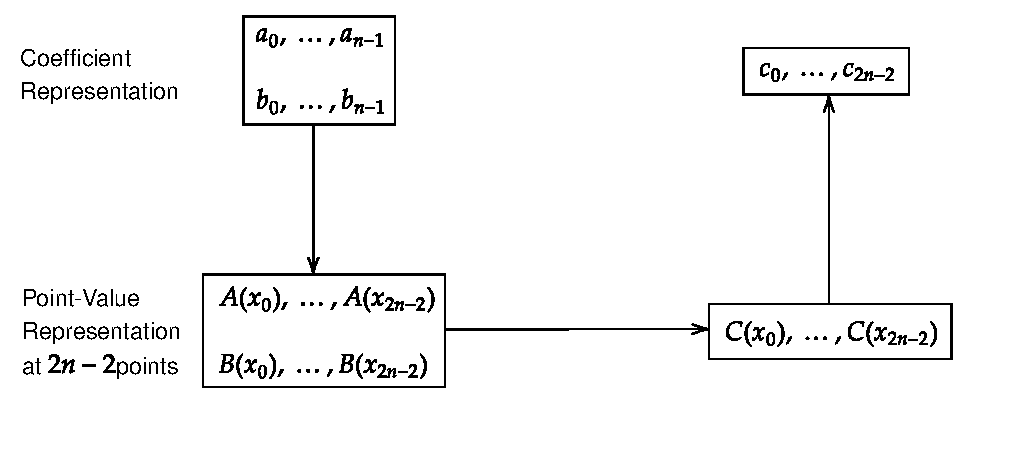
\includegraphics{images/poly-mult}
%\end{figure}
\begin{center}

\begin{tikzpicture}[node distance=3cm, thick]
	
	% Define the rectangles
	\node[draw, rectangle, minimum width=3cm, minimum height=1.5cm] (rect1) at (0, 1.5) {$ \begin{array}{l}
			a_{0} ,\dotsc ,a_{n-1}\\
			\\
			b_{0} ,\dotsc ,b_{n-1}
		\end{array}$};
	\node[draw, rectangle, minimum width=3cm, minimum height=1.5cm] at (0,-3) (rect2) {$ \begin{array}{l}
			A( x_{0}) ,\dotsc ,A( x_{2n-2})\\
			\\
			B( x_{0}) ,\dotsc ,B( x_{2n-2})
		\end{array}$};
	\node[draw, rectangle, minimum width=3cm, minimum height=1cm]  at (8, 1.5) (rect3) {$c_{0} ,\dotsc ,c_{2n-2}$};
	\node[draw, rectangle, minimum width=4cm, minimum height=1.5cm] at (8,-3) (rect4) {$C( x_{0}) ,\dotsc ,C( x_{2n-2})$};
	% Define the text blocks on the left
	\node[align=left] (text1) at (-4, 1.5) {Coefficient\\ Representation};
	\node[align=left] (text2) at (-4, -3) {Point-Value\\ Representation\\ at $\displaystyle 2n-2$ points};
	
	% Draw dotted helper lines (optional for alignment visualization)
	\draw[-Stealth] (rect1.south) -- (rect2.north);
	\draw[-Stealth] (rect2.east) -- (rect4.west);
	\draw[-Stealth] (rect4.north) -- (rect3.south);	
\end{tikzpicture}
\end{center}
\subsection{Finding Evaluations of Multiplied Polynomial}

Suppose we were given $A(x)$ and $B(x)$ evaluated at $2n-1$ distinct points $x_0,\dots, x_{2n-2}$. Then we can get $C(x)$ evaluated at $x_0,\dots, x_{2n-2}$ by $$C(x_i)=A(x_i)B(x_i)\ \forall\ i\in \llbracket 2n-2\rrbracket$$Since there are $O(n)$ many points and for each point it takes constant time to multiply we can find evaluations of $C$ at $x_0,\dots, x_{2n-2}$ in $ O(n)$ time.
\subsection{Evaluation of a Polynomial at Points}\label{fft}
\begin{question}{}{}
	Suppose there is only one point, $x_0$. Can we evaluate a $n-1$ degree polynomial $A(x)=\sum\limits_{i=0}^{n-1}a_ix^i$ at $x_0$ efficiently?
\end{question}
We can rewrite $A(x)$ as $$A(x)=a_0+x(a_1+x(a_2+x(a_3+\cdots (a_{n-1}+x(a_n))\cdots )))$$In this represent it is clear that we have to do $n$ additions and $n$ multiplications to find $A(x_0)$. Hence we can evaluate a $n-1$ degree polynomial at a point in $O(n)$ time


But we have $O(n)$ points. And if each point takes $O(n)$ time to find the evaluation of the polynomial then again it will take total $O(n^2)$ time. We are back to square one. So instead we will evaluate the polynomial in some special points and we will evaluate in all of them in $O(n\log n)$ time. So now the problem we will discuss now is to find some special $n$ points where we can evaluate a $n-1$-degree polynomial in $O(n\log n)$ time.
\parinf

\textbf{Idea:} Evaluate at roots of unity and use Fast Fourier Transform
\parinn

Assume $n$ is a power of 2. NWe have the polynomial $A(x)=\sum\limits_{i=0}^{n-1}a_ix^i$. So now consider the following two polynomials $$A^0(x)=a_0+a_2x+a_4x^2+\cdots+a_{n-2}x^{\frac{n}2-1}\qquad A^1(x)=a_1+a_3x+a_5x^2+\cdots+a_{n-1}x^{\frac{n}2-1}$$Certainly we have $$A(x)=A^0(x^2)+xA^1(x^2)$$Hence we can get $A(1)$ and $A(-1)$ by $$A(1)=A^0(1)+A^1(1)\qquad A(-1)=A^0(1)-A^1(1)$$Hence like this by evaluating two $\frac{n}2-1$ degree polynomials at one point we get evaluation of $A$ at two points. More generally for any $y\geq 0$ we have$$A(\sqrt{y})=A^0(y)+\sqrt{y}A^1(y)\qquad A(-\sqrt{y})=A^0(y)-\sqrt{y}A^1(y)$$So by recursing like this evaluating at $1,-1$ we can get evaluations of $A$ at $n^{th}$ roots of unity.

Let $$\om_n^k=n^{th}\text{ root of unity for }k\in\llbracket n-1\rrbracket = e^{i\frac{k}{n}2\pi}=\cos\lt(\frac{k}{n}2\pi\rt)+i\sin s\lt(\frac{k}{n}2\pi\rt)$$Hence we have \begin{align*}
	A\lt(\om_n^k\rt)&=A^0\lt(\om_n^{2k}\rt)+\om_n^kA^1\lt(\om_n^{2k}\rt)=A^0\lt(\om_{\frac{n}2}^{k}\rt)+\om_n^kA^1\lt(\om_{\frac{n}2}^{k}\rt)\\
	A\lt(-\om_n^k\rt)=A\lt(\om_n^{\frac{n}2+k}\rt)&=A^0\lt(\om_n^{2k}\rt)-\om_n^kA^1\lt(\om_n^{2k}\rt)=A^0\lt(\om_{\frac{n}2}^{k}\rt)-\om_n^kA^1\lt(\om_{\frac{n}2}^{k}\rt)
\end{align*}Hence now we will solve the following problem:
\begin{algoprob}
	\problemtitle{Recursive-DFT}
	\probleminput{$(a_0,\dots, a_{n-1})$ representing $(n-1)-$degree polynomial $A(x)=\sum\limits_{i=0}^{n-1}a_ix^i$}
	\problemquestion{Find the evaluations of the polynomial $A(x)$ in all $n^{th}$ roots of unity}
\end{algoprob}

\vspace*{5mm}\parinf
Since $A^0$ and $A^1$ have degree $\frac{n}2-1$ we can use recursion. Hence the algorithm is 
\begin{algorithm}\SetKwComment{Comment}{// }{}
	\DontPrintSemicolon
	\KwIn{$A=(a_0,\dots, a_{n-1})$ such that $A(x)=a_0+a_1x+\cdots+ a_{n-1}x^{n-1}$}
	\KwOut{$A(x)$ evaluated at $n^{th}$ roots of unity $\om_n^k$ for all $k\in\llbracket n-1\rrbracket$}
	\Begin{
	\If{$n==1$}{\Return{$A[0]$}}
	$A^0\longleftarrow (A[0],A[2],\dots,A[n-2])$\;	
	$A^1\longleftarrow(A[1],A[3],\dots,A[n-1])$\;
	$Y^0\longleftarrow 	\prb{Recursive-DFT}(A^0)$\;
	$Y^1\longleftarrow 	\prb{Recursive-DFT}(A^1)$\;		
	\For{$k=0$ to $\frac{n}{2}-1$}{
		
	$Y[k]\longleftarrow Y^0[k]+\om_n^kY^1[k]$\Comment*{$	A\lt(\om_n^k\rt)=A^0\lt(\om_{\frac{n}2}^{k}\rt)+\om_n^kA^1\lt(\om_{\frac{n}2}^{k}\rt)$}
	$Y\lt[k+\frac{n}{2}\rt]\longleftarrow Y^0[k]-\om_n^{\frac{n}2+k}Y^1[k]$\Comment*{$	A\lt(-\om_n^k\rt)=A^0\lt(\om_{\frac{n}2}^{k}\rt)-\om_n^kA^1\lt(\om_{\frac{n}2}^{k}\rt)$}
}
\Return{Y}
}
		\caption{\prb{Recursive-DFT}$(A)$}
	\end{algorithm}

\textbf{Time Complexity}: $T(n)=2T\lt(\frac{n}2\rt)+O(n)=O(n\log n)$.\parinn

 Therefore we can evaluate a $n-1$ degree polynomial in all the $n^{th}$ roots of unity in $O(n\log n)$ time. Hence with this algorithm we will get evaluations of the polynomial $C(x)=A(x)B(x)$ in all the $2n^{th}$ roots of unity. Now we need to interpolate the polynomial $C(x)$ from its evaluations. We will describe the process in the next subsection.
 \subsection{Interpolation from Evaluations at Roots of Unity}In this section we will show how to interpolate a $n-1$ degree polynomial from evaluations at all $n^{th}$ roots of unity. Previously we had $$\underbrace{\mat{C\lt(\om^0_n\rt)\\ C\lt(\om^1_n\rt)\\ C\lt(\om^2_n\rt)\\ \vdots\\ C\lt(\om^{n-1}_n\rt)}}_{Y}=\underbrace{\mat{1 & \om^0_n & \om ^{0\cdot 2}& \cdots & \om^{0\cdot (n-1)}\\  1 & \om^1_n & \om ^{1\cdot 2}& \cdots & \om^{1\cdot (n-1)}\\ 1 & \om^2_n & \om ^{2\cdot 2}& \cdots & \om^{2\cdot (n-1)}\\ \vdots & \vdots & \vdots & \ddots & \vdots\\ 1 & \om^{n-1}_n & \om ^{(n-1)\cdot 2}& \cdots & \om^{(n-1)\cdot (n-1)}}}_{V=\text{ Vandermonde Matrix}}\underbrace{\mat{c_0\\ c_1\\ c_2\\ \vdots \\ c_{n-1}}}_{C}$$
 
 Now vandermonde matrix is invertible since all the $n^{th}$ roots are distinct. Therefore $C=V^{-1}Y$. But we can not do a matrix inversion to interpolate the polynomial because that will take $O(n^2)$ time. Instead we have this beautiful result:
 \begin{lemma}{}{}
 	$\lt(V^{-1}\rt)_{j,k}=\frac1n\om_n^{-jk}$ for all $0\leq j,k\leq n-1$
 \end{lemma}
\begin{proof}
	Consider the matrix $n\times n$ matrix $T$ such that $(T)_{j,k}=\frac1n\om_n^{-jk}$. Now we will show $VT=I$ This will confirm that $V^{-1}=T$. Now $$\sum_{k=0}^{n-1} (V)_{i,j}\, (T)_{j,k}=\sum_{k=0}^{n-1} \om^{ij}_n\times \frac1n\om_n^{-jk}=\frac1n\sum_{k=0}^{n-1}\lt(\om^{i-k}_n\rt)^j=\begin{cases}
		\dfrac1n\dps{\sum\limits_{k=0}^{n-1}}1=1& \text{when $i=k$}\\[5mm] \dfrac1n \dfrac{1-\om^n_n}{1-\om} =0 & \text{when $i\neq k$}
	\end{cases} $$Hence in $VT$ there are $1'$s on the diagonal and rest of the locations are $0$. Hence $VT=I$. So $V^{-1}=T$.
\end{proof}
Hence we can see the inverse of the vandermonde matrix is also a vandermode matrix with a scaling factor. We will denote $y_i=C\lt(\om_n^{i}\rt)$ for $i\in\llbracket n-1\rrbracket$ since these values are given to us some how and we have to find the corresponding polynomial. Therefore we have $$\underbrace{\mat{c_0\\ c_1\\ c_2\\ \vdots \\ c_{n-1}}}_{C}=\frac1n\underbrace{\mat{1 & 1 & 1& \cdots & 1\\  1 & \om^{-1}_n & \om ^{-1\cdot 2}& \cdots & \om^{-1\cdot (n-1)}\\ 1 & \om^{-2}_n & \om ^{-2\cdot 2}& \cdots & \om^{-2\cdot (n-1)}\\ \vdots & \vdots & \vdots & \ddots & \vdots\\ 1 & \om^{-(n-1)}_n & \om ^{-(n-1)\cdot 2}& \cdots & \om^{-(n-1)\cdot (n-1)}}}_{V^{-1}}\underbrace{\mat{c_0\\ c_1\\ c_2\\ \vdots \\ c_{n-1}}}_{C}\underbrace{\mat{y_0\\ y_1\\ y_2\\ \vdots\\ y_{n-1}}}_{Y}$$
\begin{observation*}
	$nc_j=y_0+y_1\om_n^{-j}+y_2\om_n^{-2j}+\cdots+y_{n-1}\om_n^{-(n-1)j}$ for all $j\in\llbracket n-1\rrbracket$.
\end{observation*}
We can also see this situation as we have the polynomial $Y(x)=y_0+y_1x+y_2x^2+\cdots +y_{n-1}x^{n-1}$ and $c_j$ is just $Y(x)$ evaluated as $\om^{-j}_n=\om_n^{n-j}$ multiplied by $n$. Hence we just reindex the $n^{th}$ roots of unity and evaluate $Y$ $n^{th}$ roots of unity in $O(n\log n)$ time using the algorithm described in \autoref{fft}
\chapter{Dynamic Programming}
\dfnc[dynamic-prog]{Dynamic Programming}{Dynamic Programming has 3 components:\begin{enumerate}
		\item {Optimal Substructure}: Reduce problem to smaller independent problems
		\item {Recursion}: Use recursion to solve the problems by solving smaller independent problems
		\item {Table Filling}: Use a table to store the result to solved smaller independent problems.
\end{enumerate}}
\section{Longest Increasing Subsequence}
\begin{algoprob}
	\problemtitle{\prb{Longest Increasing Subsequence}}
	\probleminput{Sequence of distinct integers $A=(a_1,\dots, a_n)$}
	\problemquestion{Given an array of distinct integers find the longest increasing subsequence i.e. return maximum size set $S\subseteq[n]$ such that $\forall\ i,j\in S$, $i<j\implies a_i<a_j$}
\end{algoprob}
\subsection{\texorpdfstring{$O(n^2)$}{O(n2)} Time Algorithm}
Given $A=(a_1,\dots, a_n)$ first we will create a $n$-length array where $i^{th}$ entry stores the length and longest increasing subsequence ending at $a_i$. Certainly we have the following recursion relation$$\prb{LIS}(k)=1+\max\limits_{\substack{j<k,\  a_j<a_k}}\{\prb{LIS}(j)\}$$since if a subsequence $S\subseteq [n]$ is the longest increasing subsequence ending at $a_k$ then certainly $S-\{k\}$ is the longest increasing subsequence which ends at $a_j<a_k$ for some $j<k$. Hence, in the table we start with 1st position and using the recursion relation we fill the table from left. And after the table is filled we look for which entry of the table has maximum length. So the algorithm will be following:

\begin{algorithm}[H]
	\SetKwComment{Comment}{// }{}
	\DontPrintSemicolon
	\KwIn{Sequence of distinct integers $A=(a_1,\dots, a_n)$}
	\KwOut{Maximum size set $S\subseteq [n]$ such that $\forall\ i,j\in S$, $i<j\implies a_i<a_j$.}
	\Begin{
	Create an array $T$ of length $n$\;
	\For{$i\in[n]$}{
	$T[i][1]\longleftarrow 1+\max\{T[j][1]\colon j<k,\ a_j<a_k\}$\Comment*{Finds $\prb{LIS}[i]$}
$T[i][2]\longleftarrow T\big[T[i][1]-1\big][2]$
}	
$Index\longleftarrow \max \{T[j][1]\colon j\in[n]\}$\;
\Return{$T[Index]$}
}
\caption{\prb{LIS}$(A)$}
\end{algorithm}\parinf
\textbf{Time Complexity:} For each iteration of the loop it takes $O(n)$ time to find $\prb{LIS}[i]$. Hence, the time complexity of this algorithm is $O(n^2)$. \parinn
\subsection{\texorpdfstring{$O(n\log n)$}{O(logn)} Time Algorithm}
In the following algorithm we update the longest increasing sequence every time we see a new element of the given sequence. At any time we keep the best available sequence.
\begin{idea*}
	We can make an increasing subsequence longer by picking the smallest number for position $k$ so that there is an increasing subsequence of length $k$. Doing this we can maximize the length of the subsequence. 
\end{idea*}

\begin{Theorem}{}{}
	If $S\subseteq A$ is the longest increasing subsequence of length $t$ then for any $k\in[t]$ the number $S(k)$ is the smallest number in the subarray of $A$ starting at first  and ending at $S(k)$ such that there is an increasing subsequence of length $k$ ending at $S(k)$.
\end{Theorem}
\begin{proof}
	Assume the contrary. Suppose $\exs\ k\in[t]$ such that $k$ is the smallest number in $[t]$ such that $S(k)$ is not the smallest number to satisfy the condition. Now denote the subarray of $A$ starting at first  and ending at $S(k)$ by $A_k$. Now let $x\in A_k$ be the smallest number in $A_k$ such that there is an increasing subsequence of length $k$ ending at $x$. Certainly $x<S(k)$ by our assumption. Now since $k$ is the smallest index which does not satisfy the given condition, $\forall\ j\in[k-1]$, $S(j)$ is the smallest number in $A_j$ such that there is an increasing subsequence of length $j$ ending at $S(j)$. Then consider the subsequence $\{S(1),\dots, S(k-1),x,S(k),S(k+1),\dots, S(t)\}$. This is an increasing subsequence of $A$ and has length $t+1$. But this contradicts the minimality of $S$. Hence, contradiction \ctr Every element of $S$ follows the given condition. 
\end{proof}

So we will construct an increasing subsequence by gradually where each step this property is followed, i.e. at each step we will ensure that the sequence built at some time have the above property. So now we describe the algorithm. 
\begin{algorithm}\SetKwComment{Comment}{// }{}
	\DontPrintSemicolon
	\KwIn{Sequence of distinct integers $A=(a_1,\dots, a_n)$}	
	\KwOut{Maximum size set $S\subseteq [n]$ such that $\forall\ i,j\in S$, $i<j\implies a_i<a_j$.}
\Begin{
	Create an array $T$ of length $n$ with all entries $0$\;
	Create an array $M$ of length $n$\;
	\For{$i=1,\dots, n$}{$M[i]\longleftarrow \infty$}	
	\For{$i=1,\dots,n$}{
		$k\longleftarrow $Find the smallest index such that $M[k]\geq a_i$ using \prb{Binary-Search}\;
		$M[k]\longleftarrow a_i$\;
		$T[i]\longleftarrow M[k-1]$\Comment*{Pointer to the previous element of the sequence}
}
$l\longleftarrow $ Largest $l$ such that $M[l]$ is finite\;
Create an array $S$ of length $l$\;
\For{$i=l,\dots, 1$}{
	\If{$i=l$}{$S[l]\longleftarrow M[l]$\;
	Continue}
$S[i]\longleftarrow T\big[S[i+1]\big]$\Comment*{$T[S[i+1]]$ is pointer to previous value of sequence}
}
\Return{$(l,S)$}
}
\caption{\prb{QuickLIS}$(A)$}
\end{algorithm}\parinf

\textbf{Time Complexity:} To create the arrays and the first for loop takes $O(n)$ time. In each iteration of the for loop at line 6 it takes $O(\log n)$ time to find $k$ and rest of the operations in the loop takes constant time. So the for loop takes $O(n\log n)$ time.  Then To find $l$ and creating $S$ it takes $O(n)$ time. Then in the for loop at line 12 in each iteration it takes constant time. So the for loop at line 12 takes in total $O(n)$ time. Therefore, the algorithm takes $O(n\log n)$ time. \parinn

We will do the proof of correctness of the algorithm now.
\begin{lemma}{}{mdecreasing}
	For any index $M[k]$ is non-increasing
\end{lemma}
\begin{proof}
	Every time we change a value of $M[k]$ we replace by something smaller. So $M[k]$ is non-increasing.
\end{proof}
We denote the state of array $M$ at $i^{th}$ iteration by $M^i$. Then we have the following lemma:

\begin{lemma}{}{}
At any time $i$, $M^i[1]< M^i[2]< \cdots< M^i[n]$
\end{lemma}
\begin{proof}
We will prove this by induction on $i$. The base case follows naturally. Now for $i^{th}$ iteration suppose $M^{i-1}[k]$ is replaced by $x_i$. Then we know $\forall \ j<k$ we have $M^i[j]< x_i$. By inductive hypothesis at time $t-1$ we have $M$ as an increasing sequence. Now before replacing $M^{i-1}[k]< M^{i-1}[k+1]< \cdots M^{i-1}[n]$. Now by \lemref{th:mdecreasing} $M^{i-1}[k]$ is nonincreasing. So we still have $M^{i-1}[1]< \cdots M^{i-1}[k-1]< x_i < M^{i-1}[k+1]< \cdots < M^{i-1}[n]$. Therefore, $M^{i}$ is an increasing subsequence. Hence, but mathematical induction it holds.
\end{proof}

Now suppose at $i^{th}$ iteration $k_i$ is largest such that $M^i[k_i]<\infty$. Then $S^i$ denote the set constructed like the way we constructed at line 12--16 in the algorithm i.e. $$S^i[k_i]=M^i[k_i]\qquad \text{and}\qquad S^i[j]=T[S^i[j+1]]\quad \forall\ j\in[k_i-1]$$
\begin{lemma}{}{si-isgoodatalliterations}
	After any $i^{th}$ iteration, for $k\in[n]$ if $M^i[k]<\infty$ then $S^i[k]$ stores the smallest value in $x_1,\dots, x_i$ such that there is an increasing subsequence of size $k$ that ends in $S^i[k]$.
\end{lemma}
\begin{proof}
We will use induction on $i$. Base case: This is true after first iteration since only $M^1[1]<\infty$. So this naturally follows. 

Suppose this is true after $i$ iterations.  Now at $(i+1)^{th}$ iteration suppose $t$ be the smallest index such that $M^i[t]>x_{i+1}$. Then we have $$M^i[1]<\cdots< M^i[t-1]<x_{i+1}\leq M^i[t]<\cdots< M^i[n]\implies S^i[1]<\cdots< S^i[t-1]<x_{i+1}\leq S^i[t],\dots, S^i[k_i]$$ Now for $k\leq t-1$ it is true by the inductive hypothesis. For $k>t$ and if $M^{i+1}[k]<\infty$ then $S^{i+1}[k]$ is the smallest value in $x_1,\dots, x_{i+1}$ such that there is an increasing subsequence of size $k$ that ends in $S^{i+1}[k]$ since this was true for $i^{th}$ iteration. 

Now only the case when $k=t$ is remaining. If $S^{i+1}[k]$ does not store the smallest value in $x_1,\dots ,x_{i+1}$ to have an increasing subsequence of size $k$ ending at $S^{i+1}[k]$ then let $x_j$ was the smallest value to satisfy this condition where $j<i+1$. Then naturally $x_j<x_{i+1}$. Then $M^{i}[t]\leq x_j<x_{i+1}$. But we $t$ was the smallest number such that $M^{i}[t]\geq x_{i+1}$. Hence, contradiction. Therefore, $S^i[k]$ is the smallest value in $x_1,\dots, x_{i+1}$ to have an increasing subsequence of size $k$ ending at $S^{i+1}[k]$.  Therefore, by mathematical induction this is true for all iterations. 
\end{proof}
\begin{Theorem}{}{}
	$S$ is the longest increasing subsequence of $A$.
\end{Theorem}
\begin{proof}
	After the $n^{th}$ iteration $S^n=S$ and $k_n=l$. Hence by \lemref{th:si-isgoodatalliterations} we can say for all $k\in[l]$, $S[k]$ is the smallest number such that there is an increasing sequence of length $k$ ending at $S[k]$. Now we want to show that this increasing sequence is the longest increasing subsequence of $A$. Suppose $S$ is not the longest increasing subsequence. Let $T$ be the longest increasing subsequence of length $t>l$. Then suppose $j\leq l$ be the smallest index such that $S[j]\neq T[j]$. Now $S[j]$ is the smallest number in $x_1,\dots, x_n$ such that there is an increasing subsequence of length $j$ ending at $S[j]$. Hence, we have $S[j]<T[j]$. Now for all $i<j$ we have $S[i]=T[i]$.   Then we form this new subsequence $\hat{T}=\{T[1],T[2],\dots, T[j-1], S[j],T[j],\dots, T[t]\}$. Certainly $\hat{T}$ has length $t+1$ and it is also an increasing subsequence. But this contradicts the maximal condition of $T$. Hence, $S$ is indeed the longest increasing subsequence.
\end{proof}

\section{Optimal Binary Search Tree}
\begin{algoprob}
	\problemtitle{Optimal BST}
	\probleminput{A sorted array $A=(a_1,\dots, a_n)$ of search keys and an array of their probability distributions $P=(p(a_1),\dots, p(a_n))$}
	\problemquestion{Given array of keys $A$ and their probabilities the probability of accessing $a_i$ is $p(a_i)$ then return a binary tree  with the minimum cost where for any binary tree $T$, $\prb{Cost}(T)=\sum\limits_{i=1}^np(a_i)\cdot height\st_T(a_i)$.}
\end{algoprob}

So let $T$ be the optimal binary search tree with $a_k$ as its root for some $k\in[n]$. Let $T_l$ and $T_r$ denote the tree rooted at the left child and right child of $a_k$ in $T$ respectively. Then: \begin{align*}
	\prb{Cost}(T) & = p_k+ {\sum_{i<k}p_i\lt(1+height\st_{T_l}(a_i)\rt)}+{\sum_{i>k}p_i\lt(1+height\st_{T_r}(a_i)\rt)} = \sum_{i=1}^n p_i+\underbrace{\sum_{i<k}p_i \cdot height\st_{T_l}(a_i)}_{\prb{Cost}(T_l)}+\underbrace{\sum_{i>k}p_i \cdot height\st_{T_l}(a_i)}_{\prb{Cost}(T_r)}
\end{align*}
In general we will use the notation $\prb{OPTCost}(i,k)=\prb{Cost}(T_i^k)$ where $T_i^k$ is the optimal binary tree of the subarray $A[i\dots k]$ for any $i\leq k\leq n$.  Therefore, we arrive at the following recurrence relation $$\prb{OPTCost}(i,k)=\begin{cases}
	0&\text{when $i>k$}\\
	\sum\limits_{j=i}^k p(a_j)+\min\limits_{i\leq r\leq k}\{\prb{OPTCost}(i,r-1)+\prb{OPTCost}(r+1,k)\} & \text{otherwise}
\end{cases}$$
So the algorithm for constructing the optimal binary search tree is following:
\begin{algorithm}
\SetKwComment{Comment}{// }{}
\DontPrintSemicolon
\caption{\prb{OptimalBST}$(A,P)$}
\KwIn{A sorted array $A=(a_1,\dots, a_n)$ of search keys and an array of their probability distributions $P=(p(a_1),\dots, p(a_n))$}
\KwOut{Binary Tree $T$ with the minimum search cost, $\prb{Cost}(T)=\sum\limits_{i=1}^np(a_i)\cdot height\st_T(a_i)$}
\Begin{
	\For{$i=1,\dots, n$}{$\prb{OPTCost}[i,i]\longleftarrow (p(a_i),a_i)$, 
	$\prb{OPTCost}[0,i]\longleftarrow (0,None)$
}	
	\For{$d=2,\dots, n$}{
		\For{$i\in[n+1-d]$}{
			$minval\longleftarrow 0$ \;
			\For{$k=i+1,\dots, i+d-2$}{
				$newval\longleftarrow \prb{OPTCost}[i,k-1][1]+\prb{OPTCost}[k+1,i+d-1][1]$\;
				\If{$minval>newval$}{$minval\longleftarrow newval$\;
				$Index\longleftarrow k$}
			}
			$\prb{OPTCost}[i,i+d-1]\longleftarrow \lt(minval+\sum\limits_{k=1}^{i+d-1}p(a_k), k\rt)$\;
			$a_k.left\longleftarrow \prb{OPTCost}[i,k-1][2]$\;
			$a_k.right\longleftarrow \prb{OPTCost}[k+1,i+d-1][2]$
					
	}
}
\Return{\prb{OPTCost}$[1,n]$}
}
\end{algorithm}\parinf

\textbf{Time Complexity:} To two for loops at line 4 and line 5 takes $O(n^2)$ many iterations. Now the innermost for loop at line 7 runs $O(n)$ iterations where in each iteration it takes constant runtime. So the total running time of the algorithm is $O(n^3)$.
\chapter{Greedy Algorithm}

\section{Maximal Matching}

\begin{algoprob}
	\problemtitle{Maximal Matching}
	\probleminput{Graph $G=(V,E)$}
	\problemquestion{Find a maximal matching $M\subseteq E$ of $G$}
\end{algoprob}
Before diving into the algorithm to find a matching or maximal matching we first define what is a matching.
\begin{Definition}{Matching}{}
	For a graph $G=(V,E)$ a matching $M\subseteq E$ is a set of edges such that no two edges in $M$ are incident on same vertex.
\end{Definition}
\begin{Definition}{Maximal Matching}{}
	For a graph $G=(V,E)$ a matching $M\subseteq E$ is maximal if it cannot be extended and still by adding an edge.
\end{Definition}
There is also a maximum matching which can be easily understood from the name:
\begin{Definition}{Maximum Matching}{}
	For a graph $G=(V,E)$ a matching $M\subseteq E$ is maximum if it is maximal and has the maximum size among all the maximal matchings.
\end{Definition}

\begin{idea*}
	The idea is to create a maximal matching we will just go over each edge one by one and check if after adding them to the set $M$  the matching property still holds. 
\end{idea*}
\begin{algorithm}
	\SetKwComment{Comment}{// }{}
	\DontPrintSemicolon
	\KwIn{Graph $G=(V,E)$}
	\KwOut{Maximal Matching $M\subseteq E$ of $G$}
	\Begin{
	$M\longleftarrow \emptyset$\;
	Order the edges $E=\{e_1,\dots, e_k\}$ arbitrarily\;
	\For{$e\in E$}{\If{$M\cup \{u\}$ is matching}{$M\longleftarrow M\cup \{e\}$}}
	\Return{$M$}	
}
\caption{\prb{Maximal-Matching}}
\end{algorithm}

\begin{question}{}{}
		Do we always get the largest possible matching?
\end{question}
\solve{ Clearly algorithm output is not optimal always. We get a maximal matching sure. But we don't get a maximum matching always. For example the following graph
	\begin{center}
		\begin{tikzpicture}
			\draw (-2,0) circle (2pt) node (A){};
			\draw (0,0) circle (2pt) node (B){};
			\draw (2,0) circle (2pt) node (C){};
			\draw (4,0) circle (2pt) node (D){};
			\draw[blue, thick] (A) -- node[midway, above]{$e_1$} (B);
			\draw[red, thick] (B) -- node[midway, above]{$e_3$}(C);
			\draw[blue, thick] (C) -- node[midway, above]{$e_2$} (D);
		\end{tikzpicture}
	\end{center}
	If we start from $e_1$ we get the matching $\{e_1.e_2\}$ which is maximum matching but if we start from $e_3$ then we get only the maximal matching $\{e_3\}$ which is not maximum.}

 Since the algorithm output may not be optimal always we can ask the following question
 \begin{question}{}{}
 	How large is the matching obtained compared to the maximum matching?
 \end{question}
This brings us to the following result:

\begin{Theorem}{}{}
	For any graph $G$ let the greedy algorithm obtains the matching $M$ and the maximum matching is $M^{\star}$. Then $$|M|\geq \frac12|M^\star|$$
\end{Theorem}
\begin{proof}
	Consider an edge $e\in M^{\star}$ but $e\notin M$. Since $e$ wasn't  picked in $M$, $\exs\ e'\in M\setminus M^{\star}$ such that $e$ and $e'$ are incident on same vertex. Thus define the function $f:M^{\star}\to M$ where $$f(e)=\begin{cases}
		e&\text{when $e\in M$}\\
		e' & \text{when $e\in M^{\star}\setminus M$ where $e'\in M\setminus M^{\star}$ such that $e'\cap e\neq \emptyset$}
	\end{cases}$$

Now note that there are at most  two edges in $M^{\star}$ that are adjacent to an edge $e'\in M$ which will be mapped to $e'$. Hence $$|M\setminus M^{\star}|\geq \frac12 |M^{\star}\setminus M|$$Therefore $|f^{-1}(e')|\leq 2$ $\forall\ e'\in M$. Hence $$|M^\star|=|M\cap M^{\star}|+|M^{\star}\setminus M|\leq |M\cap M^{\star}||+2|M\setminus M^{\star}|\leq 2|M|$$Therefore we have the result $|M|\geq \frac12|M^{\star}|$. 
\end{proof}
\begin{alternate-proof} 
	Let $M_1$ and $M_2$ are two matchings. Consider the symmetric difference $M_1\triangle M_2$.  This consists of edges that are in exactly one of $M_1$ and $M_2$. Now in $M\triangle M^{\star}$ we have the following properties:
	\begin{enumerate}[label=(\alph*)]
		\item Every vertex in $M\triangle M^{\star}$ has degree $\leq 2\implies $ Each component is a path or an even cycle. 
		\item The edges of $M$ and $M^{\star}$ alternate. 
			\end{enumerate}
		Now we will prove the following property about the connected components of $M\triangle M^{\star}$.
		
\begin{center}
					
	\begin{minipage}{0.9\textwidth}
			\textit{\textbf{Claim:}}\hspace{1em} No connected component is a single edge. 
		
		\begin{proof}
			This is because let $e$ be a connected component. So the two edges $e_1,e_2$ which are adjacent to $e$,  they are either in both $M$ and $M^{\star}$ or not in $M$ and $M^{\star}$. The former case is not possible because then $e_1,e_2,e$ are all in either $M$ or $M^{\star}$ which is not possible as they do not satisfy the condition of matching. For the later case since $M^{\star}$ is maximal matching, $e\in M^{\star}$. Then $e\notin M$. That means $e,e_1,e_2\notin M$ which is not possible since $M$ is also a maximal matching. Therefore no connected component is a single edge.
		\end{proof}
	\end{minipage}
\end{center}

	
		Therefore every path has length $\geq 2$. Therefore ratio of $\#$ edges of $M$ to $\#$ edges of $M^{\star}$ in a path is $\leq 2$. And for cycles we have $\#$ edges of $M=\#$ edges of $M^{\star}$. So in every connected component $C$ of $M\triangle M^{\star}$ the ratio $\frac{|M^{\star}\cap C|}{|M\cap C|}\leq 2$. Therefore we have $$\frac{|M^{\star}|}{|M|}=\frac{|M\cap M^{\star}|+\sum\limits_{C}|M^{\star}\cap C|}{|M\cap M^{\star}|+\sum\limits_{C}|M\cap C|}\leq 2$$Hence we have $|M|\geq \frac12|M^\star|$.
		

\end{alternate-proof}
\section{Huffman Encoding}
\begin{algoprob}
	\problemtitle{Huffman Coding}
	\probleminput{$n$ symbols $A=(a-1,\dots, a_n)$ and their frequencies $P=(f_1,\dots, f_n)$ of using symbols}
	\problemquestion{Create a binary encoding such that: \begin{itemize}[itemsep=-0.2cm]
			\item Prefix Free: The code for one word can not be prefix for another code
			\item Minimality: Minimize $\prb{Cost}(b)=\sum\limits_{i=1}^n f_i\cdot \prb{Len}(b(a_i))$ where $b:A\to \{0,1\}^*$ is the binary encoding
	\end{itemize}}
\end{algoprob}

Assignment of binary strings can also be scene as placing the symbols in a binary tree where at any node $0$ means left child and $1$ means right child. Then the first condition implies that there can not be two codes which lies in the same path from the root to a leaf. I.e. it means that all the codes have to be in the leaves. Then the length of the binary coding for a symbol  is the height of the symbol in the binary tree. 

We can think the frequencies as the probability of appearing for a letter. We denote the probability of appearing of the letter $a_i$ by $p(a_i)\coloneqq \frac{f_i}{\sum\limits_{i=1}^nf_i}$. So the we can see the updated cost function $$\prb{Cost}(b)=\sum\limits_{i=1}^n p(a_i)\cdot\prb{Len}(b(a_i))$$And from now on we will see the frequencies as probabilities and cost function like this

\subsection{Optimal Binary Encoding Tree Properties}
Then our goal is to finding a binary tree with minimum cost where all the symbols are at the leaves. We have the following which establish the optimality of Huffman encoding over all prefix encodings where each symbol is assigned a unique string of bits.
\begin{lemma}{}{least-frequent-max-height}
	In the optimal encoding tree  least frequent element has maximum height.
\end{lemma}
\begin{proof}
	Suppose that is not the case. Let $T$ be the optimal encoding tree and let the least frequent element $x$ is at height $h_1$ and the element with the maximum height is $y$ with height $h_2$ and we have $h_1<h_2$.  Then we construct a new encoding tree $T'$ where we swap the positions of $x$ and $y$. So in $T'$ height of $y$ is $h_1$ and height of $x$ is $h_2$. Then $$\prb{Cost}(T)-\prb{Cost}(T')=(p(x)h_1+p(y)h_2)-(p(x)h_2+p(y)h_1)=(p(x)-p(y))(h_1-h_2)$$Since $p(x)<p(y)$ and $h_1<h_2$ we have $\prb{Cost}(T)-\prb{Cost}(T')>0$. But that is not possible since $T$ is the optimal encoding tree. So $T$ should have the minimum cost. Hence contradiction. $x$ has the maximum height.
\end{proof}

\begin{lemma}{}{complete-tree}
	The optimal encoding binary tree must be complete binary tree. (i.e. every non-leaf node has exactly $2$ children)
\end{lemma}
\begin{proof}
	Suppose $T$ be the optimal binary tree and there is a non-leaf node $r$ which has only one child at height $h$. 
	By \lmref{least-frequent-max-height} the least frequent element $x$ has the maximum height, $h_m$. 
	
	 Then consider the new tree $\hat{T}$ where we place the least frequent element at height $h$ and make it the second child of the node $r$. Then $$\prb{Cost}(T)-\prb{Cost}(\hat{T})=p(x)h_m-p(x)h=p(x)(h_m-h)>0$$But this is not possible as $T$ is the optimal binary tree and it has the minimal cost. Hence contradiction. Therefore the optimal encoding binary tree must be a complete binary tree. 
\end{proof}
\begin{lemma}{}{least-frequents-siblings}
There is an optimal binary encoding tree such that the least frequent element and the second least frequent element are siblings at the maximum height.
\end{lemma}
\begin{proof}
Let $T$ be optimal binary encoding tree. Suppose $x$, $y$ are the least frequent element and the second least frequent element. And suppose $b$, $c$  be two siblings at the maximum height of the tree (There may be many such siblings, and if so pick any such pair.). If $\{x,y\}=\{b,c\}$ we are done. So suppose not. Let the frequencies of $x,y,b,c$ are respectively $p(x),p(y),p(b),p(c)$ and heights of $x,y,b$ are $h_x,h_y$ and $h$ respectively.  WLOG assume $p(x)\leq p(y)$ and $p(b)\leq p(c)$. 

Now since we know $x,y$ have the smallest frequencies we have $p(x)\leq p(b)$ and $p(y)\leq p(c)$. And since $b,c$ have the maximum height we have $h_x,hy\geq h$. So we switch the position of $x$ with $b$ to form the new tree $T'$. And from $T'$ we swap the positions fo $y$ and $c$ to form a new tree $T''$.

\begin{center}
	\begin{tikzpicture}[
		every node/.style={font=\sffamily, align=center, line width=0.15mm},
		level 1/.style={level distance=1cm, sibling distance=2cm},  % Adjusted distance for level 1
		level 2/.style={sibling distance=2cm},   % Adjusted distance for level 2
		square/.style={draw, shape=rectangle, minimum width=0.5cm, minimum height=0.5cm, inner sep=0pt, text width=0.5cm, text centered},
		circle/.style={draw, shape=circle, minimum width=0.5cm, minimum height=0.5cm, inner sep=0pt, text width=0.5cm, text centered},
		filled/.style={fill=blue!20, , draw, line width=0.12mm},  % Style for filled nodes
		every edge/.style = {draw, latex'-latex' , line width=0.3mm, dotted,},
		parentarrow/.style={line width=0.12mm, -{latex[length=1mm, width=0.2mm, open, round]}},  % Style for arrows from nodes to children
		]
		
		% Leftmost tree
		\node[circle] (A1) {}
		child {node[circle] (B1) {}
			child {node[square] (D1) {$y$} edge from parent[parentarrow]}
			child {node[circle] (E1) {}
				child {node[square] (F1) {$c$} edge from parent[parentarrow]}
				child {node[square, filled] (G1) {$b$} edge from parent[parentarrow]}
				edge from parent[parentarrow]
			}
		edge from parent[parentarrow]
		}
		child {node[square,filled] (C1) {$x$} edge from parent[parentarrow]};
		\node[above left=0cm and 0cm of A1] (T1) {$T$};  % Label T1
		% Middle tree
		\node[circle, right=4cm of A1] (A2) {}
		child {node[circle] (B2) {}
			child {node[square, filled] (D2) {$y$} edge from parent[parentarrow]}
			child {node[circle] (E2) {}
				child {node[square, filled] (F2) {$c$} edge from parent[parentarrow]}
				child {node[square] (G2) {$x$} edge from parent[parentarrow]}
				edge from parent[parentarrow]
			}
			edge from parent[parentarrow]
		}
		child {node[square] (C2) {$b$} edge from parent[parentarrow]};
		\node[above left=0cm and 0cm of A2] (T1) {$T'$};  % Label T2
		
		% Rightmost tree
		\node[circle, right=4cm of A2] (A3) {}
		child {node[circle] (B3) {}
			child {node[square] (D3) {$c$}edge from parent[parentarrow]}
			child {node[circle] (E3) {}
				child {node[square] (F3) {$y$} edge from parent[parentarrow]}
				child {node[square] (G3) {$x$} edge from parent[parentarrow]}
				edge from parent[parentarrow]
			}
		edge from parent[parentarrow]
		}
		child {node[square] (C3) {$b$} edge from parent[parentarrow]};
		\node[above left=0cm and 0cm of A3] (T1) {$T''$};  % Label T3
		
		
		% Dotted bidirectional bent arrows between leaf nodes D and E in each tree
		\draw (C1) edge[bend left=45] (G1);
		\draw (F2) edge[bend left=45] (D2);
		
		% Arrows from leftmost tree to middle tree and from middle tree to rightmost tree
		\draw[-Latex, thick, shorten <= 1mm, shorten >= 1mm] (A1) -- (A2);
		\draw[-Latex, thick, shorten <= 1mm, shorten >= 1mm] (A2) -- (A3);
		
	\end{tikzpicture}
\captionof{figure}{Showing that the lowest probability nodes are siblings at the tree’s lowest level.} 
\label{fig:least-frequent-elm-siblings}
\end{center}

Now we will calculate how the cost changes as we go from $T$ to $T'$ and $T'$ to $T''$. First check for $T\to T'$. Almost all the nodes contribute the same except $x,b$. So we have $$\prb{Cost}(T)-\prb{Cost}(T')=(h_x\cdot p(x)+h\cdot p(b))-(h_x\cdot p(b)+h\cdot p(x))=(p(b)-p(x))(h-h_x)\geq 0$$Therefore swapping $x$ and $b$ does not increase the cost and since $T$ is the optimal binary encoding tree the cost doesn't decrease either. Therefore the costs are equal. Hence $T'$ is also an optimal tree. 

Similarly we calculate cost for going from $T'$ to $T''$ we have $$\prb{Cost}(T')-\prb{Cost}(T'')=(h_y\cdot p(y)+h\cdot p(c))-(h_y\cdot p(c)+h\cdot p(y))=(p(c)-p(y))(h-h_y)\geq 0$$Therefore swapping $y$ and $c$ also does not increase the cost and since $T'$ is the optimal binary encoding tree the cost doesn't decrease either. Therefore the costs are equal. Hence $T''$ is also an optimal tree. Hence $T''$ is the optimal tree where the least frequent element and second last frequent element are siblings.
\end{proof}




By the \lmref{complete-tree} and \lmref{least-frequents-siblings} we have that the least frequent element and the second least frequent element are siblings and they have the maximum height.

%\begin{Theorem}{}{replace-less-variable-case}
%Let $T_n$ be any optimal binary encoding tree following \lmref{least-frequents-siblings} (i.e. lowest probability symbols $x$ and $y$ are siblings at the deepest level). Let $T_{n-1}$ be the tree that results by replacing these two leaf nodes for $x,y$  and their parent with a single leaf node $z$ of probability $p(z)=p(x)+p(y)$. Then $$\prb{{Cost}}(T_n)=\prb{Cost}(T_{n-1})+p(z)$$
%\end{Theorem}
%\begin{proof}
%	Let $h$ be the heights of $x$ and $y$ in $T_n$. Clearly $z$ is in height $h-1$ in $T_{n-1}$. Since $z$ replaces $x$ and $y$ the costs of the two trees satisfies \begin{align*}
%		\prb{Cost}(T_n)&=\prb{Cost}(T_{n-1})-(\text{\prb{Cost} due to $z$ in \prb{Cost}$(T_{n-1})$} + (\text{\prb{Cost} due to $x$ and $y$ in \prb{Cost}$(T_{n})$})\\
%		& =\prb{Cost}(T_{n-1})-p(z)\cdot (d-1)+(p(x)+p(y))\cdot d\\
%		& = \prb{Cost}(T_{n-1})-p(z)\cdot (d-1)+p(z)\cdot d\\
%		& = \prb{Cost}(T_{n-1})+p(z)
%	\end{align*}
%\end{proof}

\begin{observation*}
	The cost of the trees $T_n$ and $T_{n-1}$ differ only by the fixed term $p(z)=p(x)+p(y)$ which does not depend on the tree's structure. Therefore minimizing the cost for $T_n$ is equivalent to minimizing the cost of $T_{n-1}$.
\end{observation*}
\begin{Theorem}{}{replace-less-variable-case}
	Given an instance with symbols $\mcI$: \begin{center}
		\begin{tabular}{ccccccccc}
			$a_1$, & $a_2$, & $\cdots$, & $a_i$, & $\cdots$, & $a_j$, & $\cdots$, & $a_n$ & with probabilities\\
			$p(a_1)$, & $p(a_2)$, & $\cdots$, & $p(a_i)$, & $\cdots$, & $p(a_j)$, & $\cdots$, & $p(a_n)$ &
		\end{tabular} 
	\end{center}
	such that $a_i$, $a_j$ are the least frequent and second least frequent elements respectively. Consider the instance with $n-1$ symbols $\mcI'$:
	\begin{center}
		\begin{tabular}{ccccccccccc}
			$a_1$, & $a_2$, & $\cdots$, & $a_{i-1}$, & $a_{i+1}$,& $\cdots$, & $a_{j-1}$,& $a_{j+1}$, & $\cdots$, & $a_n$, & $z$ \\
			$p(a_1)$, & $p(a_2)$, & $\cdots$, & $p(a_{i-1})$,&$p(a_{i+1})$  & $\cdots$, & $p(a_{j-1})$,& $p(a_{j+1})$, & $\cdots$, & $p(a_n)$, & $p(a_i)+p(a_j)$ 
		\end{tabular} 
	\end{center}
	Let $T'$ be the optimal tree for this instance $\mcI'$. Then there is an optimal tree for the original instance $\mcI$ obtained from $T'$ by replacing the leaf of $b$ by an internal node with children $a_i$ and $a_j$.
\end{Theorem}
\begin{proof}
	We will prove this by contradiction. Suppose $\hat{T}$ is optimal for $\mcI$. Then $\prb{Cost}(\hat{T})<\prb{Cost}(T)$. In $\hat{T}$ we know $a_i$ and $a_j$ are siblings by \lmref{least-frequents-siblings}. Now consider $\hat{T}'$ for instance $\mcI'$ where we merge $a_i,a_j$ leaves and their parent into a leaf for symbol $z$. 
	
	\begin{center}
		\usetikzlibrary{fit}
		\begin{tikzpicture}[
			every node/.style={font=\sffamily, align=center, line width=0.15mm},
			level 1/.style={level distance=1cm, sibling distance=2cm},  % Adjusted distance for level 1
			level 2/.style={sibling distance=2cm},   % Adjusted distance for level 2
			square/.style={draw, shape=rectangle, minimum width=0.5cm, minimum height=0.5cm, inner sep=0pt, text width=0.5cm, text centered},
			circle/.style={draw, shape=circle, minimum width=0.5cm, minimum height=0.5cm, inner sep=0pt, text width=0.5cm, text centered},
			filled/.style={fill=blue!20, , draw, line width=0.12mm},  % Style for filled nodes
			every edge/.style = {draw, latex'-latex' , line width=0.3mm, dotted,},
			parentarrow/.style={line width=0.12mm, -{latex[length=1mm, width=0.2mm, open, round]}},  % Style for arrows from nodes to children
			dottedoval/.style={draw, line width=0.3mm, densely dotted, inner sep=0.2mm, ellipse, minimum width=1cm, minimum height=1.5cm}, % Style for the dotted oval shape
			]
			
			% Leftmost tree
			\node[circle] (A1) {}
			child {node[circle] (B1) {}
				child {node[circle] (D1) {} edge from parent[parentarrow]}
				child {node[circle, filled] (E1) {}
					child {node[square, filled] (F1) {$a_i$} edge from parent[parentarrow]}
					child {node[square,filled] (G1) {$a_j$} edge from parent[parentarrow]}
					edge from parent[parentarrow]
				}
				edge from parent[parentarrow]
			}
			child {node[circle] (C1) {} edge from parent[parentarrow]};
			\node[above left=0cm and 0cm of A1] (T1) {${T}$};  % Label T1
			% Middle tree
			\node[circle, left=4cm of A1] (A2) {}
			child {node[circle] (B2) {}
				child {node[circle] (D2) {} edge from parent[parentarrow]}
				child {node[square, filled] (E2) {$z$}}
				edge from parent[parentarrow]
			}
			child {node[circle] (C2) {} edge from parent[parentarrow]};
			\node[above left=0cm and 0cm of A2] (T1) {${T}'$};  % Label T2
			\draw[-Latex, thick, shorten <= 1mm, shorten >= 1mm] (A2) -- (A1);
			% Dotted oval shape containing E1, F1, and G1
			\node[dottedoval, fit=(E1)(F1)(G1), yshift=-0.15cm] (Oval) {};
			
			% Arrow from dotted oval to B1
			\draw[-latex, dottedoval] (E2) to[out=-90,in=-150] (Oval);
		\end{tikzpicture}
	\end{center}
	
	Then $$\prb{Cost}(\hat{T}')=\prb{Cost}(\hat{T})-p(a_i)-p(a_j)<\prb{Cost}(T)-p(a_i)-p(a_j)=\prb{Cost}(T')$$This contradicts the fact that $T'$ is optimal binary encoding tree for $\mcI'$. Hence $T$ is optimal.
\end{proof}




\subsection{Algorithm}
\begin{idea}
	We are going to build the tree up from the leaf level. We will take two characters $x,y$, and ``merge” them into a single character, $z$, which then replaces $x$ and $y$ in the alphabet. The character $z$ will have  probability
	equal to the sum of $x$ and $y$’s probabilities. Then we continue recursively building the code on
	the new alphabet, which has one fewer character.
\end{idea}

Since we always need the least frequent element and the second least frequent element we have to use the data structure called \prb{Min-Priority Queue}. So the following algorithm uses a \prb{Min-Priority Queue} $Q$ keyed on the probabilities to identify the two least frequent objects. 

%\newpage 
\begin{algorithm}
	\SetKwComment{Comment}{// }{}
	\DontPrintSemicolon
	\KwIn{Set of $n$ symbols $A=\{a_1,\dots, a_n\}$ and their probabilities $P=\{p_1,\dots, p_n\}$}
	\KwOut{Optimal Binary Encoding $b:A\to \{0,1\}^*$ for $A$ with minimum $\prb{Cost}(b)=\sum\limits_{i=1}^n p(a_i)\cdot\prb{Len}(b(a_i))$.}
	\Begin{
	$n\longleftarrow |A|$\;
	$Q\longleftarrow$ \prb{Min-Priority Queue}\;
	\For{$x\in A$}{\prb{Insert}$(Q,x)$}
	\For{$i=1,\dots n-1$}{$z\longleftarrow $ New internal tree node\;
		$x\longleftarrow $ \prb{Extract-Min}$(Q)$,		$y\longleftarrow $ \prb{Extract-Min}$(Q)$\;
	$left[z]\longleftarrow x$, 
$right[z]\longleftarrow y$\;
$p(z)\longleftarrow p(x)+p(y)$\;
$\prb{Insert}(Q,z)$
}
\Return{Last element left in $Q$ as root}
}
\caption{\prb{Huffman-Encoding}$(A,P)$}
\end{algorithm}

\parinf
\textbf{Time Complexity:} To create the priority queue it takes $O(n)$ time in line 4-5. Then for each iteration of the for loop in line 6 the \prb{Extract-Min} operation takes $O(\log n)$ time and then to insert an element it also takes $O(\log n)$ time. Hence each iteration takes $O(\log n)$ time. Since the for loop has $n-1=O(n)$ many iterations the running time for the algorithm is $O(n\log n)$. 

\begin{remark}
	We can reduce the running time to $O(n\log\log n)$ by replacing the binary min-heap with a van Emde Boas tree.
\end{remark}

\begin{Theorem}{Correctness of Huffman's Algorithm}{}
	The above Huffman's algorithm produces an optimal prefix code tree
\end{Theorem}
\begin{proof}
	We will prove this by induction on $n$, the number of symbols. For base case $n=1$. There is only one tree possible.
	
	For $n=k$ we know that by \lmref{least-frequents-siblings} and \lmref{least-frequent-max-height} that the two symbols $x$ and $y$ of lowest probabilities are siblings and they have the maximum height. Huffman's algorithm replaces these nodes by a character $z$ whose probability is the sum of their probabilities. Now we have 1 less symbols. So by inductive hypothesis Huffman's algorithm computes the optimal binary encoding tree for the $k-1$ symbols. Call it $T_{n-1}$. Then the algorithm replaces $z$ with a parent node with children $x$ and $y$ which results in a tree $T_n$ whose cost is higher by a fixed amount $p(z)=p(x)+p(y)$. Now since $T_{n-1}$ is optimal by \thmref{replace-less-variable-case} we have $T_n$ is also optimal.
\end{proof}
\section{Matroids}
\dfn{Matroid}{A matroid $M=(E,\mcI)$ has a ground set $E$ and a collection $I$ of subsets of $E$ called the \textit{Independent Sets} st\begin{enumerate}
		\item Downward Closure: If $Y\in \mcI$ then $\forall \ X\subseteq Y$, $X\in \mcI$.
		\item Exchange Property: If $X,Y\in \mcI$, $|X|<|Y|$ then $\exs\ e\in Y-X$ such that $X\cup \{e\}$ also written as $X+e\in \mcI$
\end{enumerate}}
An element $x\in E$ extends $A\in\mcI$ if $A\cup \{x\}\in\mcI$. And $A$ is maximal if no element can extend $A$.
\begin{lemma}{}{}
	If $A,B$ are maximal independent set, then $|A|=|B|$ i.e. all maximal independent sets are also maximum
\end{lemma}
\begin{proof}
	Suppose $|A|\neq |B|$. WLOG assume $|A|>|B|$. Then by the exchange property $\exs\ e\in A-B$ such that $B\cup \{e\}\in\mcI$. But we assumed that $B$ is maximal independent set. Hence contradiction. We have $|A|=|B|$.
\end{proof}
\parinf

\textbf{Base:} Maximal Independent sets are called bases.

\textbf{Rank of $\boldsymbol{S\in I}$:} $\max\{|X|\colon X\subseteq S, X\in I\}$

\textbf{Rank of a Matroid:} Size of the base.

\textbf{Span of $\boldsymbol{S\in I}$:} $\{e\in E\colon rank(S)=rank(S+e)\}$



\subsection{Examples of Matroid}
\begin{itemize}[label=$\bullet$]
\item \textbf{Uniform Matroid:} Given $E=\{e_1,\dots, e_n\}$, and $k\in\bbZ_0$ take $\mcI=\{S\subseteq E\colon |S|\leq k\}$
\begin{lemma}{}{}
	$M=(E,\mcI)$ defined as above is a matroid
\end{lemma}
\begin{proof}
	\begin{enumerate}[label=\bfseries\tiny\protect\circled{\small\arabic*}]
		\item Downward Closure: $A\in \mcI$, $B\subseteq A\implies |B|\leq k\implies B\in \mcI$
		\item Exchange Property: $A,B\in\mcI,\ |B|<|A|\leq k\implies |B|<k\implies \forall\ e\in A-B,\ |B\cup \{e\}|\leq k\implies B\cup \{e\}\in \mcI$
	\end{enumerate}
Therefore $M$ is a matroid
\end{proof}
\item \textbf{Partition Matroid:} Given $E$, $\{P_1,\dots, P_l\}$ such that $E=\bigsqcap\limits_{i=1}^lP_i$ and $k_1,\dots, k_l\in\bbZ_0$ then take $$\mcI=\{S\subseteq E\colon \forall\ k\in[l],\ |S\cap P_j|\leq k_j\}$$
\begin{lemma}{}{}
	$M=(E,\mcI)$ defined as above is a matroid
\end{lemma}
\begin{proof}
		\begin{enumerate}[label=\bfseries\tiny\protect\circled{\small\arabic*}]
		\item Downward Closure: $A\in \mcI$, $B\subseteq A\implies \forall\ j\in[l]\ |B\cap P_j|\leq |A\cap P_j|\leq k_j\implies B\in \mcI$
		\item Exchange Property: $A,B\in\mcI,\ |B|<|A|\implies \exs \ j\in[l],\ |B\cap P_j|< |A\cap P_j|\leq k_j\implies e\in (A\cap P_j)-{(B\cap P_j)}, \ |(B\cup\{e\})\cap P_j|=|B\cap P_j|+1\leq k\implies B\cup \{e\}\in\mcI$
	\end{enumerate}Therefore $M$ is a matroid
\end{proof}
\item \textbf{Laminar Matroid:} Given $E$, $\sL=\{L_1,\dots,L_l\}$ such that $\forall\ i,j\in [l]$, either $L_i\subseteq L_j$ or $L_i\supseteq L_j$ or $L_i\cap L_j=\emptyset$ and also given $k_1,\dots, k_l\in \bbZ_0$. Then take $$\mcI=\{S\subseteq E\colon \forall \ j\in[l],\ |S\cap L_j|\leq k_j\}$$For any $L\in\sL$ we denote $k(L)$ be the given number corresponding to $L$.
\begin{lemma}{}{laminar-matroid}
	$M=(E,\mcI)$ defined as above is a matroid
\end{lemma}
\begin{proof}
	\begin{enumerate}[label=\bfseries\tiny\protect\circled{\small\arabic*}]
		\item Downward Closure: $A\in \mcI$, $B\subseteq A\implies \forall\ j\in[l]\ |B\cap L_j|\leq |A\cap L_j|\leq k_j\implies B\in \mcI$
		\item Exchange Property: \parinn Let $A,B\in \mathcal{I}$ with $|B|<|A|$.	If there exists $e\in A\backslash B$ such that $e\notin L$ for any $L\in\sL$, then $|(B+e)\cap L|=|B\cap L|\leq k(L)$ for any $L\in\sL$.
		
		Hence assume that for each $e\in A\backslash B$ there exists $L\in\sL$ with $e\in L$.
		For each $e\in A\backslash B$, let $\sL_e$ be the collection of $L\in\sL$ with $e\in L$.
		For each $e\in A\backslash B$ and any $L\in\sL\backslash\sL_e$, we have $|(B+e)\cap L|=|B\cap L|\leq k(L)$.
		
		Hence it remains to show that there exists $e\in A\backslash B$ such that $|(B+e)\cap L|\leq k(L)$ for any $L\in\sL_e$.
		Note that $\sL_e$ is a chain, as $\sL$ is a laminar.
		Let $\sL'=\{L_{e_1},\ldots,L_{e_l}\}$ be the collection of inclusion-wise maximal sets in $\sL$ such that $|B\cap L_{e_i}|\leq k(L_{e_i})$ with $e_i\in A\backslash B$.
		Then $L_{e_i}\cap L_{e_j}=\emptyset$. Moreover, $|A|>|B|$ and $|A\cap L_{e_i}|\leq k(L_{e_i})$ imply that $|A\backslash (\cup L_{e_i})|>|B\backslash (\cup L_{e_i})|$. Hence there $\exs\ e_i$ such that $|A\cap L_{e_i}|>|B\cap L_{e_i}|$.
		
		 Now we take a look at the chain $\sL_{e_i}$. For brevity we will use $e$ instead of $e_i$. So in the chain $\sL_e=\{L_1,\dots, L_n\}$ such that  we have $$L_n\supseteq L_{n-1}\supseteq \cdots \supseteq L_2\supseteq L_1$$Then take $i\in[n]$ to be the largest index such that $|A\cap L_i|\leq |B\cap L_i|$. There will be such index because otherwise we will have $|A|\leq |B|$ which is not possible. Then take $e^*\in (A\cap L_{i+1})-(L_i\cup B)$. Such an $e^*$ will exist because $|A\cap L_{i+1}|>|A\cap L_{i+1}|\implies A\cap (L_{i+1}- L_{i}\neq \emptyset$ and also $A\cap (L_{i+1}- L_{i}\not\subseteq B\cap (L_{i+1}-L_i)$ because otherwise we will have $$|A\cap L_{i+1}|=|A\cap (L_{i+1}- L_{i}|+|A\cap L_{i+1}|\leq |B\cap (L_{i+1}-L_i)|+|B\cap L_i|=|B\cap L_{i+1}|$$which is not possible. Hence there exists $e^*$ such that $e^*\in (A\cap L_{i+1})-(L_i\cup B)$. Therefore take $B^*=B\cup \{e^*\}$. Then for all $j< i$ we have $B^*\cap L_j=B\cap L_j$ so we don't have a problem there. Now for all $j\geq i$ we have $|A\cap L_j|>|B\cap L_j|$. Hence now $|B^*\cap L_j|\leq |B\cap L_j|+1\leq |A\cap L_j|\leq k(L_j)$. Therefore we have $B^*\in\mcI$. Hence the exchange property follows.
	\end{enumerate}
Therefore $M$ is a matroid.
\end{proof}
\item \textbf{Graphic Matroid:} Given a graph $G=(V,E)$ $E$ is the ground set and take $$\mcI=\{E'\subseteq E\colon E'\text{ is acyclic} \}$$
\begin{lemma}{}{}
	$M=(E,\mcI)$ defined as above is a matroid
\end{lemma}
\begin{proof}
	\begin{enumerate}[label=\bfseries\tiny\protect\circled{\small\arabic*}]
		\item Downward Closure: If a set of edges $S$ is acyclic then naturally any subset of edges of $S$ is also acyclic. Hence downward closure property follows.
		\item Exchange Property: $A,B\in\mcI,$ and $ |B|<|A|$. Let $G_1,\dots, G_k$ are the connected components due to $B$. For each component $G_i$, we have $|G_i\cap A|\leq |G_i\cap B|$ since each component is a tree and $B$ has maximum number of edges for that component. Then $A$ contains an edge $e$ connecting $2$ components $G_i$ and $G_j$. Then $B\cup \{e\}\in \mcI$. 
	\end{enumerate}Therefore $M$ is a matroid
\end{proof}

\item \textbf{Linear Matroid:} Given a $m\times n$ matrix $M\in \bbZ^{m\times n}$, $E=[n]$ and take $$\mcI=\{S\subseteq E\colon \text{Columns of $M$ corresponding to $S$ are linearly independent} \}$$
\begin{lemma}{}{}
	$M=(E,\mcI)$ defined as above is a matroid
\end{lemma}
\begin{proof}
	\begin{enumerate}[label=\bfseries\tiny\protect\circled{\small\arabic*}]
		\item Downward Closure: $A\in \mcI$, $B\subseteq A$. Subset of linearly independent set is also linearly independent. Hence $B\in \mcI$. 
		\item Exchange Property: $A,B\in\mcI,\ |B|<|A|$. Then take span $\la A\ra$ over $\bbQ$. Now we know a set of integral vectors are linearly independent over integers if and only if they are linearly independent over rationals. Hence $|A|=\dim _{\bbQ}\la A\ra> \dim _{\bbQ}\la B\ra|B|$. Hence we can extend $B$ by an element $e\in A-B$ such that $\la B\cup \{e\}\ra =|B|+1$. Hence $B\cup \{e\}\in \mcI$.
	\end{enumerate}Therefore $M$ is a matroid
\end{proof}
This matroid is also called Metric Matroid.
\end{itemize}
\subsection{Finding Max Weight Base}
\begin{algoprob}
	\problemtitle{Max Weight Base}
	\probleminput{A matroid $M=(E,I)$ is given as an input as an oracle and a weight function $W:E\to \bbR$.}
	\problemquestion{Find the maximum weight base of the matroid.}
\end{algoprob}

We will solve this using greedy algorithm.

\begin{algorithm}[H]
	\KwIn{A matroid $M=(E,I)$ is given as an input as an oracle and a weight function $W:E\to \bbR$.}
	\KwOut{Find the maximum weight base of the matroid}
	\DontPrintSemicolon
	\Begin{
		Assume $w(1)\geq \cdots \geq w(n)$\;
		$S\leftarrow \emptyset$\;
		$I\leftarrow \{S\}$\;
		\For{$i=1$ to $n$}{\If{$S+i\in I$}{$S\leftarrow S+i$}}
		\Return{S}
	}
	\caption{\prb{Max-Weight-Base}($E,W$)}
\end{algorithm}
%\subsubsection{Correctness Analysis and Characterization}
\thm{}{The above algorithm outputs a maximum weight base}
\begin{proof}	Let $M$ be a matroid. We will prove that this greedy algorithm works by inducting on $i$. At any iteration $i$ we need to prove the following claim:
	
\begin{claimwidth}
			
	\begin{claim}{}{}
		At any iteration $i$ there is a max weight base $B_i$ such that $S_i\subseteq B_i$ and $B_i\setminus S_i\subseteq \{i+1,\dots, n\}$.
	\end{claim}
	
\begin{proof}
	Base case: $S=\emptyset$. So for base case the statement is true trivially. Assume that the statement is true up to $(i-1)$ iterations.\parinn
	
	Now $S_{i-1}\subseteq B_{i-1}$ where $B_{i-1}$ is a maximum weight base and $B_{i-1}-S_{i-1}\subseteq \{i,\dots, n\}$. Now three cases arise:
	\begin{enumerate}[label=\bfseries Case \arabic*:,leftmargin=1.5cm]
		\item If $i\in B_{i-1}$ then $S_{i-1}+i\subseteq B_{i-1}$. Therefore $S_{i-1}+i$ is independent. So now $B_i=B_{i-1}$ and $S_i=S_{i-1}+i$ and $B_i-S_i\subseteq \{i+1,\dots, n\}$.
		\item If $i\notin B_{i-1}$ and $S_{i-1}+i\notin \mcI$. Then $S_i=S_{i-1}$ and $B_i=B_{i-1}$. And $B_i-S_i\subseteq \{i+1,\dots , n\}$.
		\item If $i\notin B_{i-1}$ but $S_{i-1}+i\in \mcI$. Then $S_i=S_{i-1}+i$. Now $S_i$ can be extended to a $B'$ by adding all but one element of $B_{i-1}$. So $|B'|=|B_{i-1}|$. Let the element which is not added is $j\in B_{i-1}$. So $B'=B_{i-1}+i-j$. $$wt(B')=Wt(B_{i-1})-wt()+wt(i)$$But we have $wt(i)\geq wt(j)$. So $wt(B')\geq wt(B_{i-1})$. Now since $B_{i-1}$ has maximum weight we have $wt(B')=wt(B_{i-1})$. Then our $B_i=B'$. So $B_i-S_i\subseteq \{i+1,\dots, n\}$.
	\end{enumerate}
	Hence the claim is true for the $i$th stage as well. Therefore the claim is true.
\end{proof}
\end{claimwidth}

\begin{claimwidth}
	\begin{claim}{}{}
	At any iteration, $T_i=\{t_1,\dots, t_k\}$, then $T_i$ is a maximum weight independent set with at most $i$ elements
\end{claim}
\begin{proof}
	We will prove by induction. Base Case: $i=0$. Then $T_i=\emptyset$. So the statement follows naturally.
	
	Assume $T_{i-1}$ is maximum weight independent set with at most $i-1$ elements. Now for a contradiction, say $\hat{T}_i\in\mcI$ of size at most $i$ with strictly larger weight than $T_i$. Then $\exs\ x\in \hat{T_i}-T_{i-1}$ such that $T_{i-1}\cup \{x\}\in \mcI$. Then we have $$wt(\hat{T}_i-x)\leq wt(T_{i-1})$$by inductive hypothesis. The only element that extend $T_{i-1}$ are those $t_{i-1}$. Therefore $wt(x)\leq wt(t_i)$. Hence we have $$wt(\hat{T}_i-x)+wt(x)\leq wt(T_{i-1}wt(t_i)\implies wt(\hat{T}_I)\leq wt(T_i)$$But we assumes $wt(\hat{T}_i)>wt(T_i)$. Hence contradiction. 
\end{proof}
\end{claimwidth}

	\parinn 
	
	Therefore using the claims, after the algorithm finished we have no elements left to check, so the current set has the maximum weight which is also an independent set. So the algorithm successfully returns a maximum weight base.
\end{proof}
\subsection{Job Selection with Penalties}

\begin{algoprob}
	\problemtitle{Find Feasible Schedule}
	\probleminput{Set $J$ of $n$ jobs with deadlines $d_1,\dots, d_n$ and rewards $w_1,\dots, w_n$}
	\problemquestion{Each jobs unit time and we have a single machine to process their jobs. Give a feasible schedule of jobs with maximum reward}
\end{algoprob}

First lets define what is a schedule and what is a feasible schedule:

\begin{Definition}{Feasible Schedule}{}
	For a subset $S$ of jobs:
	\begin{enumerate}[label=\bfseries\tiny\protect\circled{\small\arabic*}]
	\item A schedule is an ordering of $S$
	\item A feasible schedule is one where one job in $S$ gets finished by deadline.
	\item A set $S\subseteq J$ is feasible if $S$ has a feasible schedule.
	\end{enumerate}
\end{Definition}\parinn

Now  for any $S\subseteq J$, and $t\in\bbZ_+$, define $N_t(S)=\{j\in S\colon d_j\leq t\}$. Then we have the following lemma:
\begin{lemma}{}{job-schedule}
	\Tfae
	\begin{enumerate}[label=\bfseries\tiny\protect\circled{\small\arabic*}]
		\item $S$ is feasible
		\item $\forall\ t\in\bbZ_t$, $|N_t(S)|\leq t$
		\item The schedule that orders jobs by deadline is feasible
	\end{enumerate}
\end{lemma}
\begin{proof}

\begin{itemize}[wide]
	\item[$3\implies 1$:] This follows naturally
	\item[$1\implies 2$:] Suppose not. Then $\exs$ $t$ such that $|N_t(S)|>t$. Then by time $t$, greater than $t$ many jobs have to be completed. But  $S$ is feasible so every job is finished by deadlines and each job takes unit take. Hence by time $t$, more than $t$ jobs can not finished. Hence contradiction.
	\item[$2\implies 3$:] The schedule orders the jobs by deadline. We induction on $t$. For $t=1$ we have $|N_1(S)|\leq 1$. Hence by $t=1$ at most one job is completed. At $t=1$ the jobs are completed within deadline. Suppose till time $t-1$ the jobs are completed within deadlines. At time $t$ we have $|N_t(S)|\leq t$. Therefore all the jobs with deadlines $\leq t$ in $S$. So they all can be completed within time $t$ in any order. Therefore if we complete the jobs with deadline $<t$ first then also we can complete all the jobs with deadline $t$ within time $t$. Hence at time $t$ all the jobs are completed within their deadlines. Hence by mathematical induction at time $t=n$ all the jobs are completed within deadline. Therefore the schedule orders jobs by deadline then it is a feasible schedule.
\end{itemize}
\end{proof}
\begin{lemma}{}{}
	Consider $M=(J,\mcI)$ where $S$ is feasible $\implies S\in \mcI$. Then $M$ is a matroid. (Assume that no two jobs have same deadline)
\end{lemma}
\begin{proof}
	Suppose $D\coloneqq $ the maximum of all deadlines. Consider the set $$\sL=\{N_t(J)\colon t\in [D]\}$$Then take $\mcI'=\{S\subseteq J\colon |N_t(S)|\leq t\ \forall t\in [D]\}$. By \lmref{laminar-matroid} $M=(J,\mcI')$ is a laminar matroid. And by \lmref{job-schedule} $\mcI'$ is the set of feasible schedules. Therefore $\mcI'=\mcI$. Hence $M$ is a matroid.
\end{proof}
\begin{alternate-proof}
	\begin{enumerate}[label=\bfseries\tiny\protect\circled{\small\arabic*}]
		\item Downward Closure: If $S\in\mcI$ then $S$ is feasible. Then for any subset $T$ of $S$ all the jobs are completed within deadlines since $S$ is feasible. So $T\in \mcI$.
		\item Exchanges Property: Given $S,T\in\mcI$ and $|T|<|S|$. Now order $S$ and $T$ by deadlines. Let $j$ be the job with largest deadline that is not in $S$ i.e. $j=\underset{i\in S\setminus T}{\max}d_i$. Then we claim that $T\cup \{j\}\in\mcI$. \parinn
		
		Now define $$T^<=\{i\in T\colon d_i<d_j\}\qquad T^>=\{i\in T\colon d_i>d_j\}$$And also similarly define$$S^<=\{i\in S\colon d_i<d_j\}\qquad S^>=\{i\in S\colon d_i>d_j\}$$As we defined $j$ we have $T^>=S^>$. Since we have $|S|>|T|$ we have $|S^<|\geq |T^<|$.  
		
		Now if $T\cup \{j\}$ is not feasible then $\exs\ t$ such that $|N_t(T\cup \{j\})|>t$. Since $T$ is feasible we have $|N_t(T)|\leq t$. Hence $t\geq d_j$ otherwise $N_t(T\cup \{j\})=N_t(T)$. But then $$|N_t(T\cup \{j\})|=|T^<|+1+|\{i\in T\cup \{j\}\colon d_j<d_i\leq t\}|\leq |S^<|+1+|\{i\in S\cup \{j\}\colon d_j<d_i\leq t\}|=|N_t(S)|\leq t$$Therefore we obtain $|N_t(T\cup \{j\})|\leq t$. Hence contradiction. Therefore $T\cup \{j\}$ is feasible.
	\end{enumerate}
\end{alternate-proof}



\chapter{Dijkstra Algorithm with Data Structures}
\begin{algoprob}
	\problemtitle{Minimum Weight Path}
	\probleminput{Directed Graph $G=(V,E)$, $s\in V$ is source and $W=\{w_e\in \bbZ_+\colon e\in E\}$}
	\problemquestion{$\forall\ v\in V-\{s\}$ find minimum weight path $s\rightsquigarrow v$.}
\end{algoprob}

This is the problem we will discuss in this chapter. In this chapter we will often use the term `shortest distance' to denote the minimum weight path distance. One of the most famous algorithm for finding out minimum weight paths to all vertices from a given source vertex is Dijkstra's Algorithm
\section{Dijkstra Algorithm}
We will assume that the graph is given as adjacency list. Dijkstra Algorithm is basically dynamic programming. Suppose $\delta(v)$ is the shortest path distance from $s\rightsquigarrow v$.  Then we have the following relation:
$$\delta(v)=\min\limits_{u:(u,v)\in E}\{\delta(u)+e(u,v)\}$$And suppose for any vertex $v\in V-\{s\}$, $dist(v)$ be the distance from $s$ estimated by the algorithm at any point. This is why  Dijkstra's algorithm maintains a set $S$  of vertices   whose final shortest-path weights from the source $s$ have already been determined. The algorithm repeatedly selects the vertex $u\in V-S$ with minimum shortest-path estimate and estimates the distances of neighbors of $u$. So here is the algorithm:

\begin{algorithm}
	\SetKwComment{Comment}{// }{ }
	\DontPrintSemicolon
	\KwIn{Adjacency Matrix of digraph $G=(V,E)$, source vertex $s\in V$ and weight function $W=\{w_e\in \bbZ_+\colon e\in E\}$}
	\KwOut{$\forall\ v\in V-\{s\}$ minimum weight path from $s\rightsquigarrow v$}
	\Begin{
		$S\longleftarrow \emptyset$, $U\longleftarrow V$\;
		$dist(s)\longleftarrow 0$, $\forall\ v\in V-\{s\}$, $dist(v)\longleftarrow\infty$\;
		\While{$U\neq \emptyset$}{
			$u\longleftarrow \min\limits_{u\in U} dist(u)$ and remove $u$ from $U$\;
			$S\longleftarrow S\cup \{u\}$\;
			\For{$e=(u,v)\in E$}{$dist(v)\longleftarrow \min\{dist(v), dist(u)+w(u,v)\}$}
		}
	}
	\caption{\prb{Dijkstra}$(G,s,W)$}
\end{algorithm}

Here below we give an example of how the Dijkstra algorithm works:
%\begin{center}

\begin{figure}[h]
	\centering
	\begin{tikzpicture}[
			node distance = 12mm and 14mm,
			every state/.append style = {inner sep=0pt, fill=gray!10,
					minimum size=7mm},
			every edge/.style = {draw, -Stealth, bend angle=15},
			auto=right,
		]

		%
		%	\draw[blue!20, line width=5pt] 	(s1) to                     (s2);
		%
		\begin{scope}[shift={(-6,0)}]
			\node (s1) [state,fill=gray!30,label={left:$s$}]         {$\boldsymbol{0}$};
			\node (s2) [state, above right=of s1]   {$\boldsymbol{\infty}$};
			\node (s3) [state, right=of s2]         {$\boldsymbol{\infty}$};
			\node (s4) [state, below right =of s1]   {$\boldsymbol{\infty}$};
			\node (s5) [state, right=of s4]          {$\boldsymbol{\infty}$};
			\draw   (s1) edge [ "$10$"]             (s2)
			(s1) edge ["$5$"]						(s4)
			(s2) edge ["$1$"]             			(s3)
			(s2) edge [bend right, "$2$"]			(s4)
			(s3) edge [bend right, "$4$"] 			(s5)
			(s5) edge [bend right,"$6$"]  			(s3)
			(s5) edge [bend left=80,looseness=1.2,  "$7$", swap]	(s1)
			(s4) edge ["$2$"] 						(s5)
			(s4) edge ["$9$"]						(s3)
			(s4) edge [bend right, "$3$"]			(s2);
		\end{scope}

		\begin{scope}[shift={(0,0)}]
			\node (s1) [state,fill=gray!30,label={left:$s$},fill=black,text=white]         {$\boldsymbol{0}$};
			\node (s2) [state, above right=of s1]   {$\boldsymbol{10}$};
			\node (s3) [state, right=of s2]         {$\boldsymbol{\infty}$};
			\node (s4) [state,fill=gray!30, below right =of s1]   {$\boldsymbol{5}$};
			\node (s5) [state, right=of s4]          {$\boldsymbol{10}$};
			\draw[blue!20, line width=5pt] (s1) -- (s2);
			\draw[blue!20, line width=5pt] (s1) -- (s4);
			\draw   (s1) edge [ "$10$"]             			(s2)
			(s1) edge ["$5$"]									(s4)
			(s2) edge ["$1$"]             						(s3)
			(s2) edge [bend right, "$2$"]						(s4)
			(s3) edge [bend right, "$4$"] 						(s5)
			(s5) edge [bend right,"$6$"]  						(s3)
			(s5) edge [bend left=80,looseness=1.2,"$7$", swap]	(s1)
			(s4) edge ["$2$"] 									(s5)
			(s4) edge ["$9$"]									(s3)
			(s4) edge [bend right, "$3$"]						(s2);

		\end{scope}

		\begin{scope}[shift={(6,0)}]
			\node (s1) [state,label={left:$s$},fill=black,text=white]         {$\boldsymbol{0}$};
			\node (s2) [state, above right=of s1]   {$\boldsymbol{8}$};
			\node (s3) [state, right=of s2]         {$\boldsymbol{13}$};
			\node (s4) [state, below right =of s1,fill=black,text=white]   {$\boldsymbol{5}$};
			\node (s5) [state, right=of s4,fill=gray!30]          {$\boldsymbol{7}$};
			\draw[red!20, line width=5pt] (s1) -- (s4);
			\draw[blue!20, line width=5pt] (s4) to [bend right=15] (s2);
			\draw[blue!20, line width=5pt] (s4) -- (s5);
			\draw[blue!20, line width=5pt] (s4) -- (s3);
			\draw   (s1) edge [ "$10$"]             			(s2)
			(s1) edge ["$5$"]									(s4)
			(s2) edge ["$1$"]             						(s3)
			(s2) edge [bend right, "$2$"]						(s4)
			(s3) edge [bend right, "$4$"] 						(s5)
			(s5) edge [bend right,"$6$"]  						(s3)
			(s5) edge [bend left=80,looseness=1.2,"$7$", swap]	(s1)
			(s4) edge ["$2$"] 									(s5)
			(s4) edge ["$9$"]									(s3)
			(s4) edge [bend right, "$3$"]						(s2);
		\end{scope}

		\begin{scope}[shift={(-6,-6)}]
			\node (s1) [state,fill=gray!30,label={left:$s$},fill=black,text=white]      {$\boldsymbol{0}$};
			\node (s2) [state,fill=gray!30, above right=of s1]   						{$\boldsymbol{8}$};
			\node (s3) [state, right=of s2]        		 								{$\boldsymbol{13}$};
			\node (s4) [state, below right =of s1,fill=black,text=white]   				{$\boldsymbol{5}$};
			\node (s5) [state, right=of s4,fill=black,text=white]          {$\boldsymbol{7}$};
			\draw[red!20, line width=5pt] (s1) -- (s4);
			\draw[red!20, line width=5pt] (s4) to [bend right=15] (s2);
			\draw[red!20, line width=5pt] (s4) -- (s5);
			\draw[blue!20, line width=5pt] (s5) to [bend right=15] (s3);
			\draw[blue!20, line width=5pt] (s5) to [bend left=80,looseness=1.3]	(s1);
			\draw   (s1) edge [ "$10$"]             			(s2)
			(s1) edge ["$5$"]									(s4)
			(s2) edge ["$1$"]             						(s3)
			(s2) edge [bend right, "$2$"]						(s4)
			(s3) edge [bend right, "$4$"] 						(s5)
			(s5) edge [bend right,"$6$"]  						(s3)
			(s5) edge [bend left=80,looseness=1.3,"$7$", swap]	(s1)
			(s4) edge ["$2$"] 									(s5)
			(s4) edge ["$9$"]									(s3)
			(s4) edge [bend right, "$3$"]						(s2);
		\end{scope}

		\begin{scope}[shift={(0,-6)}]
			\node (s1) [state,fill=gray!30,label={left:$s$},fill=black,text=white]         {$\boldsymbol{0}$};
			\node (s2) [state, above right=of s1,fill=black,text=white]   {$\boldsymbol{8}$};
			\node (s3) [state, right=of s2,fill=gray!30]         {$\boldsymbol{9}$};
			\node (s4) [state, below right =of s1,fill=black,text=white]   {$\boldsymbol{5}$};
			\node (s5) [state, right=of s4,fill=black,text=white]          {$\boldsymbol{7}$};
			\draw[red!20, line width=5pt] (s1) -- (s4);
			\draw[red!20, line width=5pt] (s4) to [bend right=15] (s2);
			\draw[red!20, line width=5pt] (s4) -- (s5);
			\draw[red!20, line width=5pt] (s5) to [bend right=15] (s3);
			\draw[blue!20, line width=5pt] (s2) -- (s3);
			\draw   (s1) edge [ "$10$"]             			(s2)
			(s1) edge ["$5$"]									(s4)
			(s2) edge ["$1$"]             						(s3)
			(s2) edge [bend right, "$2$"]						(s4)
			(s3) edge [bend right, "$4$"] 						(s5)
			(s5) edge [bend right,"$6$"]  						(s3)
			(s5) edge [bend left=80,looseness=1.3,"$7$", swap]	(s1)
			(s4) edge ["$2$"] 									(s5)
			(s4) edge ["$9$"]									(s3)
			(s4) edge [bend right, "$3$"]						(s2);
		\end{scope}

		\begin{scope}[shift={(6,-6)}]
			\node (s1) [state,fill=gray!30,label={left:$s$},fill=black,text=white]         {$\boldsymbol{0}$};
			\node (s2) [state, above right=of s1,fill=black,text=white]   {$\boldsymbol{8}$};
			\node (s3) [state, right=of s2,fill=black,text=white]         {$\boldsymbol{9}$};
			\node (s4) [state, below right =of s1,fill=black,text=white]   {$\boldsymbol{5}$};
			\node (s5) [state,fill=gray!30, right=of s4,fill=black,text=white]          {$\boldsymbol{7}$};
			\draw[red!20, line width=5pt] (s1) -- (s4);
			\draw[red!20, line width=5pt] (s4) to [bend right=15] (s2);
			\draw[red!20, line width=5pt] (s4) -- (s5);
			%	\draw[red!20, line width=5pt] (s5) to [bend right=15] (s3);	
			\draw[red!20, line width=5pt] (s2) -- (s3);
			\draw   (s1) edge [ "$10$"]             			(s2)
			(s1) edge ["$5$"]									(s4)
			(s2) edge ["$1$"]             						(s3)
			(s2) edge [bend right, "$2$"]						(s4)
			(s3) edge [bend right, "$4$"] 						(s5)
			(s5) edge [bend right,"$6$"]  						(s3)
			(s5) edge [bend left=80,looseness=1.3,"$7$", swap]	(s1)
			(s4) edge ["$2$"] 									(s5)
			(s4) edge ["$9$"]									(s3)
			(s4) edge [bend right, "$3$"]						(s2);
		\end{scope}
	\end{tikzpicture}
	\caption{The execution of Dijkstra’s algorithm. The source s is the leftmost vertex. The 	shortest-path estimates appear within the vertices, and shaded edges indicate predecessor values. Black vertices are in the set $S$ and at any iteration of while loop the shaded vertex has the minimum value. At any iteration the red edges are the edges considered in minimum weight path from $s$ using only vertices in $S$.}
\end{figure}

Suppose at any iteration $t$, let $dist_t(v)$ denotes the distance $v$ from $s$ calculated by algorithm for any $v\in V$ and $S^{(t)}$ denote the content of $S$ at $t^{th}$ iteration. In order to show that the algorithm correctly computes the distances we prove the following lemma:
\begin{Theorem}{}{}
	For each $v\in S^{(t)}$, $\dl(v)=dist_t(v)$ for any iteration $t$.
\end{Theorem}
\begin{proof}
	We will prove this induction. Base case is $|S^{(1)}|=1$. $S$ grows in size. Then only time $|S^{(1)}|=1$ is when $S^{(1)}=\{s\}$ and $d(s)=0=\dl(s)$. Hence, for base case this is correct.

	Suppose this is also true for $t-1$. Let at $t^{th}$ iteration the vertex $u\in V-S$ is picked. By induction hypothesis for all $v\in S^{(t)}-\{u\}$, $dist_t(v)=dist_{t-1}(v)=\dl(v)$. So we have to show that $dist_{t}(u)=\dl(u)$.

	Suppose for contradiction the shortest path from $s\rightsquigarrow u$ is $P$ and has total weight $=\dl(u)=w(P)<dist_t(u)$. Now $P$ starts with vertices from $S^{(t)}$ by eventually leaves $S$. Let $(x,y)$ be the first edge in $P$ which leaves $S$ i.e. $x\in S$ but $y\notin S$. By inductive hypothesis $dist_t(x)=\dl(x)$. Let $P_y$ denote the path $s\rightsquigarrow y$ following $P$. Since $y$ appears before $u$ we have $$w(P_y)=\dl(y)\leq \dl(u)=w(P)$$Now $$dist_t(y)\leq dist_t(x)+w(x,y)$$ since $y$ is adjacent to $x$. Therefore $$dist_t(y)\leq dist_t(x)+w(x,y)=\dl(y)\leq dist_t(y)\implies dist_t(y)=\dl(y)$$Now since both $u,y\notin S^{(t)}$ and the algorithm picked up $u$ we have $\dl(u)<dist_t(u)\leq dist_t(y)=\dl(y)$. But we can not have both $\dl(y)\leq \dl(u)$ and $\dl(u)<\dl(y)$. Hence contradiction. Therefore $\dl(u)=dist_t(u)$. Hence by mathematical induction for any iteration $t$, for all $v\in S^{(t)}$, $\dl(v)=dist_t(v)$.
\end{proof}

Therefore, by the lemma  after all iterations $S$ has all the vertices with their shortest distances from $s$ and henceforth the algorithm runs correctly.

Now in the algorithm there are two things which needed to keep track of. At every iteration of the while loop we needed to find the vertex $u$ which had the minimum distance from the source vertex, and we needed to update the distance of a vertex by decreasing the value as needed. So after the decrease we need to update the minimum distance vertex. So in any data structure used to do these two operations we need the following things:\begin{itemize}[label=$\bullet$]
	\item Need to store: $\forall\ v\in V$, $dist(v)$
	\item Operations: \begin{itemize}
		      \item \textsc{Extract-Min}: Gives the vertex with minimum distance in $v$ and remove from the data structure.
		      \item \textsc{Decrease-Key}: For vertex $v$ reduce $dist(v)$ to $k$.
	      \end{itemize}
\end{itemize}\parinf

In the algorithm we called \textsc{Extract-Min} $n$ times and \textsc{Decrease-Key} $m$ times.\parinn

\section{Data Structure 1: Linear Array}
So naively we can use a linear array of size $n$ where each element of the array corresponds to a vertex. Each element of the array is a tuple of flag of being in $U$ and the value $dist(v)$. To \textsc{Extract-Min} it takes $O(n)$ time since we need to compare all the elements and for \textsc{Decrese-Key} it takes $O(1)$ time. Therefore Dijkstra takes $n\cdot O(n)+O(m)=O(n^2)$ time.

\section{Data Structure 2: Min Heap}
A binary heap data structure is an array object that we can view as ``Almost complete binary'' tree (ACB tree). Each node of the tree corresponds to an element of the array. The tree is completely filled on all levels except possibly the lowest which is filled from the left up to a point.

Let the ACB tree has height $h$. Then heap  is completely field until height $h-1$ i.e. every vertex up to  level $h-2$ has exactly two children and a node at height $h-1$ is missing a child then:\begin{itemize}
	\item Either both children are missing or only right child are missing.
	\item Every vertex to the right of the node is missing both children.
\end{itemize}An ACB tree height $h$ is represented as an array of size $2^h-1$. For vertex $v$ stored at $A[i]$, the left child of $A$ is at $A[2i]$ and the right child is at $A[2i+1]$ and the parent of $A$ is at $A\lt[\lfloor\frac{i}{2}\rfloor\rt]$.
\begin{figure}[h!]
	\centering
	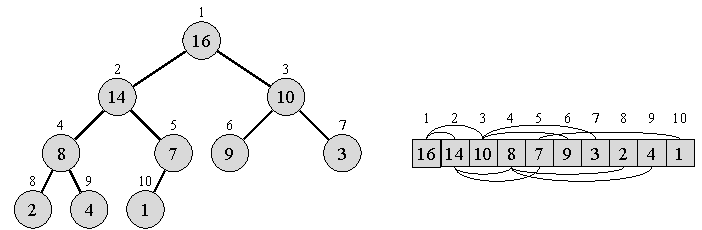
\includegraphics[width=0.9\textwidth]{images/Heap.pdf}
	\caption{A max-heap viewed as an ACB tree (left) and as an array (right)}
\end{figure}

Here we will study min-heap where the value of the children is more than the value of its parent.
\subsection{Initialization}
We create an array $A$ of size $n$. Initially we store the key value of every node to be $\infty$. And for the root $s$ we store $s.\emph{key}=0$.
\subsection{Extracting the Minimum}
For minimum, we already know the root of the heap or the first element of $A$ is the minimum. But after extracting the minimum we need to balance the heap so that it gets the properties of min-heap back. For that we replace the root with the right most element in the array $A$. Then balance the heap by moving it down if one of the child has \emph{key} smaller than \emph{node.key} and keep doing it until both child is larger.
\begin{algorithm}[]
	\caption{\textsc{Extract-Min}$(A)$}
	\SetKwComment{Comment}{// }{}
	\DontPrintSemicolon
	$t\longleftarrow A.\emph{size}$\;
	$Minval\longleftarrow A[1].\emph{key}$\;
	$A[1]\longleftarrow A[t]$\;
	$t\longleftarrow t-1$, $i\longleftarrow 1$\;
	\While{True}{
		\If{$2i\leq t$}{
			$left-val\longleftarrow A[2i].\emph{key}$\;
		}
		\Else{
			\Return{$minval$}\Comment*{No left child i.e. already at leaf}
		}
		\If{$2i+1\leq t$}{
			$right-val\longleftarrow A[2i+1].\emph{key}$
		}
		\Else{
			$right-val\longleftarrow \infty$\Comment*{No right child}
		}
		\If{$left-val\leq right-val$ and $A[i].\emph{key}<left-val$}{
			$curr\_elm\longleftarrow A[i]$\;
			$A[i]\longleftarrow A[2i]$\;
			$U[2i]\longleftarrow curr\_elm$\;
			$i\longleftarrow 2i$
		}
		\ElseIf{$right-val<left-val$}{
			$curr\_elm\longleftarrow A[i]$\;
			$A[i]\longleftarrow A[2i+1]$\;
			$U[2i+1]\longleftarrow curr\_elm$\;
			$i\longleftarrow 2i+1$
		}
		\Else{
			Break
		}
		\Return{$minval$}
	}
\end{algorithm}

In this algorithm for extracting min each time the height of the new root node increases by one at each iteration of the while loop. Hence, this takes at most $O(\log n)$ time.
\subsection{Decreasing Key of a Node}
After decreasing the \emph{key} of a node it may have smaller key than it's parent node. So move it upward i.e. replace with its parent node, and we keep doing it until the parent node has smaller value than it.
\begin{algorithm}[]
	\caption{\textsc{Decrease-Key}$(A,i,k)$}
	\DontPrintSemicolon
	$t\longleftarrow A.\emph{size}$\;
	$A[i]\longleftarrow k$\;
	\While{$i>1$ and $A[i].\emph{key}<A\lt[\lfloor\frac{i}{2}\rfloor\rt].\emph{key}$}{
		$curr\_elm\longleftarrow A[i]$\;
		$A[i].\emph{key}\longleftarrow A\lt[\lfloor\frac{i}{2}\rfloor\rt]$\;
		$A\lt[\lfloor\frac{i}{2}\rfloor\rt]\longleftarrow curr\_elm$\;
		$i\longleftarrow\lt\lfloor\frac{i}{2}\rt\rfloor$
	}
\end{algorithm}
Here again at each iteration of the while loop the height decreases by $1$. Hence, this takes at most $O(\log n)$ time.
\subsection{Time Complexity Analysis of Dijkstra}
Both \textsc{Extract-Min} and \textsc{Decrease-Key} takes $O(\log n)$ time for a min-heap. Now in a Dijkstra algorithm there are $n$ calls for \textsc{Extract-Min} and $m$ calls for \textsc{Decrease-Key}. Therefore, the total time taken by Dijkstra is $O(n\log n)+O(m\log n)=O(m\log n)$. But this is better when $m=o\lt(\frac{n^2}{\log n}\rt)$. Now we will show an improvement of min-heap where the amortized cost of \textsc{Extract-Min} is $O(\log n)$ and amortized cost of \textsc{Decrease-Key} is constant. But first we will take a detour of explaining amortized analysis.
\section{Amortized Analysis}
In amortized analysis, we average the time required to perform a sequence of data-structure operations over all the operations performed. With amortized analysis, we can show that the average cost of an operation is small, if we average over a sequence of operations, even though a single operation within the sequence might be expensive.
\nt{Amortized analysis in not average-case analysis as  amortized analysis guarantees the average performance of each operation in the worst case}

Consider the following algorithm:
\begin{algorithm}[]
	\caption{Amortized Analysis}
	\DontPrintSemicolon
	\KwIn{$n$}
	\Begin{
		$t\longleftarrow 0$, $X(0)\longleftarrow 0^n$\;
		\While{True}{
			$t\longleftarrow t+1$\;
			$X(t)\longleftarrow X(t-1)+1$
		}
	}
\end{algorithm}
Now the number of bit flips in this process is $1,2,1,3,\dots, n,\dots$. At any point the number of bit flips can be at most $n$. In the worst case an operation has cost $n$. We want to compute the average cost for an operation. We will show that starting from $X(0)=0^n$ the average cost is at most $2$. Furthermore, we will show 3 different proofs of this.
\begin{lemma}{}{}
	The total  cost of bit flips for $t$ operations is at most $2t$.
\end{lemma}
\begin{proofmany}{1 (Counting)}
	In $t$ operations:
	\begin{center}
		\begin{tabular}{rl}
			$n^{th}$ bit gets flipped:     & $t$ times                                                    \\
			$(n-1)^{th}$ bit gets flipped: & $\lfloor\frac{t}2\rfloor$ times (when $n^{th}$ bit is 1)     \\
			$(n-2)^{th}$ bit gets flipped: & $\lfloor\frac{t}4\rfloor$ times (when $(n-1)^{th}$ bit is 1) \\
			$\vdots$\hspace{1cm}           & \hspace{1cm}$\vdots$
		\end{tabular}
	\end{center}
	Therefore the total number of bit flips we get is $\leq t\lt(1+\frac12+\frac14+\cdots\rt)\leq 2t$.
\end{proofmany}

Now we will give a proof using the accounting method. In the accounting method of amortized analysis, we assign each operation an amortized cost that may differ from its actual cost. If the amortized cost is higher, the excess is stored as credit on data structure objects; if lower, credit is used to cover the gap. This way, expensive operations can be balanced by cheaper ones, and different operations may have different amortized costs.

\begin{proofmany}{2 (Charging)}
	Suppose every operation costs $2$ Rs. \begin{itemize}
		\item Every change from $0\to 1$ charges $1$ Rs and store $1$ Rs.
		\item Every change from $1\to 0$ charges $2$ Rs.
	\end{itemize}
	Now as you can see to change from $1\to 0$ that bit was previously changed from $0\to 1$. So to change from $1\to 0$ we can use the stored $1$ Rs. Hence, in average every operation costs exactly $0$ to $1$ Rs. Since there are $t$ operations total number of bit flips is at most $2t$.
\end{proofmany}

In the next proof we will analyze by computing a necessary potential function. After each operation we can calculate the potential difference.

\begin{proofmany}{3 (Potential)}
	Consider the potential function $\Phi(i)=\#$1's in $X(i)$. Let at $i^{th}$ operation $t_i$ bits were flipped from $1\to 0$. Now any operation flips at most $1$ bit from $0\to 1$. Therefore, number of bit flips in $i^{th}$ operation is at most $t_i+1$. Therefore, we have $$\Phi(i)\leq \Phi(i-1)-t_i+1$$since the number of $1$'s in $\Phi(i)$ is decreased by $t_i$ many $1\to 0$ flips and then $1$ flip from $0\to 1$. Therefore, the cost at $i^{th}$ operation is at most $\Phi(i-1)-\Phi(i)+2$. Hence, the total number of bit flips in $t$ operations is $\Phi(0)-\Phi(t)+2t\leq 2t$.
\end{proofmany}

Hence, after $t$ operations the total number of bit flips is at most $2t$. Therefore, on average the cost per operation is at most $2$. Hence, the amortized cost of the operation is $2$. So we will use such amortized analysis on the next data structure to optimize the run time of Dijkstra Algorithm.
\section{Data Structure 3: Fibonacci Heap}
Instead of keeping just one Heap we will now keep an array of Heaps. We will also discard the idea of binary trees. We will now use a data structure which will take the benefit of the faster time of both the data structure. I.e.
\begin{center}
	\begin{tabular}{c|c|c}
		               & \prb{Extract-Min}                                       & \prb{Decrease-Key}                                 \\
		Linear Array   & $O(n)$                                                  & $\mathcolor{red}{\boxed{\mathcolor{black}{O(1)}}}$ \\
		Min-Heap       & $\mathcolor{red}{\boxed{\mathcolor{black}{O(\log n)}}}$ & $O(\log n)$                                        \\[2mm]
		Fibonacci Heap & $O(\log n)^*$                                           & $O(1)^*$
	\end{tabular}
\end{center}
The * is because  in Fibonacci Heap the amortized time taken by \prb{Extract-Min} is  $O(\log n)$.

Since Fibonacci heap is an array of heaps there is a \emph{rootlist} which is the list of all the roots of all the heaps in the Fibonacci heap. There is a \emph{min-pointer} which points to the root with the minimum key. For each node in the Fibonacci heap we have a pointer to its parent and  we keep 3 variables. The 3 variables are \emph{degree}, \emph{size} and \emph{lost} where \emph{lost} is a Boolean Variable. \begin{itemize}
	\item For any node $x$ in the Fibonacci heap the $x.\emph{degree}$ is the number of children $x$ has.
	\item $x.\emph{size}$ is the number of nodes in the tree rooted at $x$.
	\item $x.\emph{lost}$ is 1 if and only if $x$ has lost a child before.
\end{itemize} Why any node will lose a child that explanation we will give later. With this set up let's dive into the data structure.

\begin{figure}[h!]
	\centering
	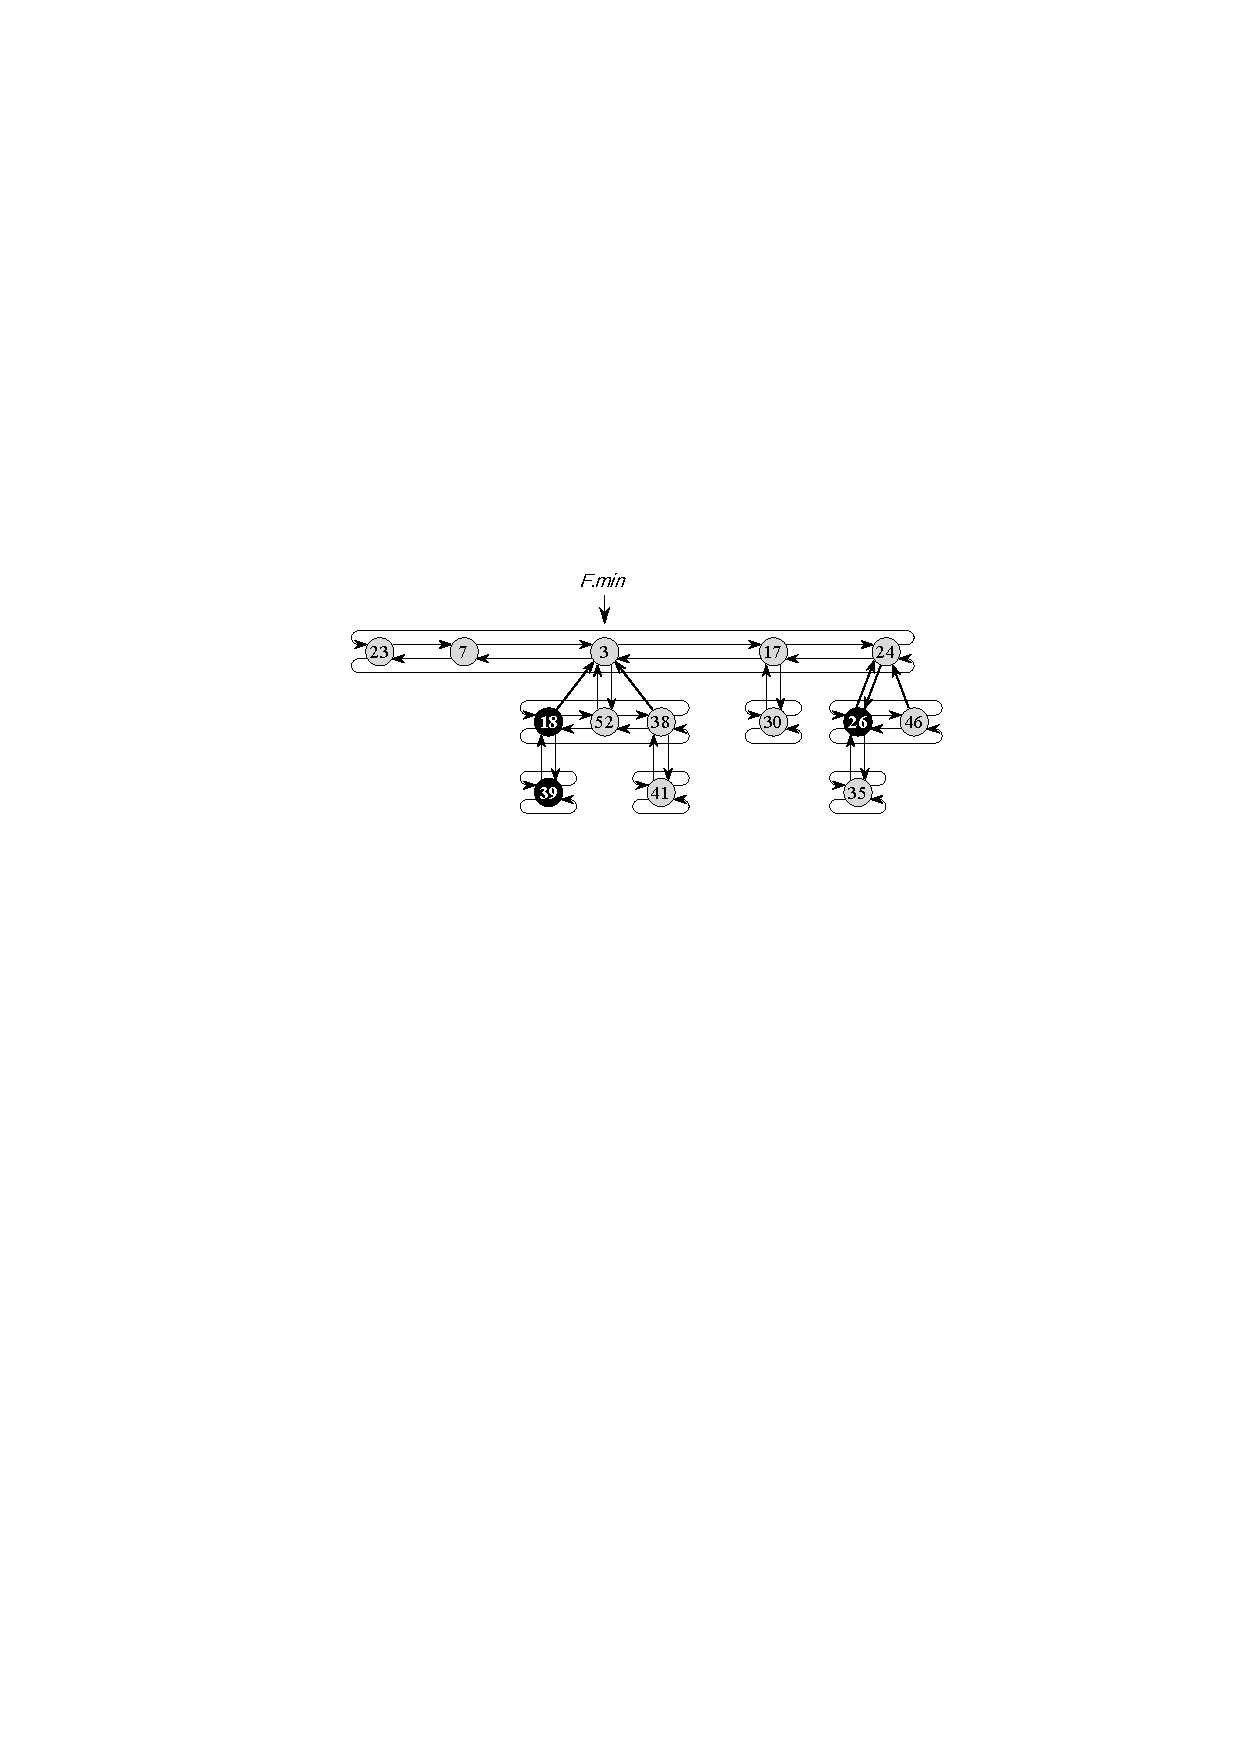
\includegraphics{images/Fibheap1.pdf}
	\caption{A Fibonacci Heap with 5 heaps in the rootlist}
\end{figure}
\subsection{Inserting Node}
To insert a node we call the \prb{Fib-Insert} function and in the function the algorithm initiates the node with setting up all the pointers and variables then add the node to the \emph{rootlist}.\parinf

\begin{minipage}{0.45\textwidth}
	\begin{algorithm}[H]
		\DontPrintSemicolon
		\caption{\textsc{Fib-Create-Node}$(v)$}
		$x.\emph{degree}\longleftarrow 0$\;
		$x.\emph{parent}\longleftarrow None$\;
		$x.\emph{child}\longleftarrow None$\;
		$x.\emph{lost}\longleftarrow 0$\;
		$x.\emph{key}\longleftarrow v$\;
		\Return{$x$}
	\end{algorithm}
\end{minipage}\hfill
\begin{minipage}{0.45\textwidth}
	\begin{algorithm}[H]
		\DontPrintSemicolon
		\caption{\textsc{Fib-Insert}$(F,v)$}
		$x\longleftarrow \textsc{Create-Node}(v)$\;
		\If{$F.\min==None$}{
			$F.\emph{rootlist}\longleftarrow [x]$\;
			$F.\min\longleftarrow x$\;
		}
		\Else{
			$F.\emph{rootlist}.\emph{append}(x)$\;
			\If{$x.key<F.\min.key$}{
				$F.min\longleftarrow x$
			}
		}
	\end{algorithm}
\end{minipage}

All of this can be done in $O(1)$ time. Therefore, to insert a node in the Fibonacci heap it takes $O(1)$ time.
\subsection{Union of Fibonacci Heaps}
To unite to Fibonacci heaps $F_1$ and $F_2$ we simply concatenate the root lists of $F_1$ and $F_2$ and then determine the new minimum node.
\begin{algorithm}
	\DontPrintSemicolon
	\caption{\textsc{Fib-Union}$(F_1,F_2)$}
	$F\longleftarrow \textsc{Make-Fib-Heap}$\;
	$F.\min\longleftarrow F_1.\min$\;
	$F.\emph{rootlist}\longleftarrow F_1.\emph{rootlist} ++ F_2.\emph{rootlist}$\;
	\If{$F_2.\min<F_1.\min$}{
		$F.\min\longleftarrow F_2.\min$
	}
	\Return{$F$}
\end{algorithm}
All the operations here can be done in constant time. Hence, \textsc{Fib-Union} takes $O(1)$ time.
\subsection{Extracting the Minimum Node}
The \textsc{Fib-Extract-Min} function extracts the minimum node from the Fibonacci heap $F$ and then rearranges the heap array. It works by first making a root node out of each of the minimum node's children and removing the minimum node from the rootlist. It then consolidates the root list by linking roots of equal degree until at most one root remains of each degree.
\begin{center}
	\begin{minipage}{0.45\textwidth}
		\begin{algorithm}[H]
			\caption{\textsc{Fib-Extract-Min}$(F)$}
			\DontPrintSemicolon
			$z\longleftarrow F.\min$\;
			\If{$z\neq None$}{
				\For{$x\in z.\emph{child}$}{
					$F.\emph{rootlist}.\emph{append}(x)$\;
					$x.\emph{parent}\longleftarrow None$
				}
				Remove $z$ from $F.\emph{rootlist}$\;
				\If{$z==z.\emph{right}$}{
					$F.\min\longleftarrow None$\;
				}
				\Else{
					$F.\min\longleftarrow z.\emph{right}$
					\emph{consolidate}($F$)
				}
			}
			\Return{$z$}
		\end{algorithm}
		\vspace{2.8cm}

		\begin{algorithm}[H]
			\caption{\textsc{Fib-Heap-Link}$(H,y,x)$}
			\DontPrintSemicolon
			Remove $y$ from $F.\emph{rootlist}$\;
			$y.\emph{parent}\longleftarrow x$\;
			$y.\emph{lost}\longleftarrow 0$
		\end{algorithm}
	\end{minipage}\hfill
	\begin{minipage}{0.5\textwidth}
		\begin{algorithm}[H]
			\caption{\textsc{Consolidate}$(F)$}
			\DontPrintSemicolon
			Initialize array $A[0,\dots, D(n)]$ with \emph{None} elements.\;
			\For{$x\in F.\emph{rootlist}$}{
				$d\longleftarrow x.\emph{degree}$\;
				\If{$A[d]==None$}{
					$A[d]\longleftarrow x$
				}
				\While{$A[d]\neq None$}{
					$y\longleftarrow A[d]$\;
					\If{$y.\emph{key}<x.\emph{key}$}{
						Exchange $x$ with $y$
					}
					\emph{Fib-Heap-Link}$(F,y,x)$\;
					$A[d]\longleftarrow None$, $d\longleftarrow d+1$\;
				}
				$A[d]\longleftarrow x$
			}
			$F.\min\longleftarrow None$\;
			\For{$i=0$ to $D$}{
				\If{$A[i]\neq None$}{
					\If{$F.\min==None$}{
						$F.\emph{rootlist}\longleftarrow [A[i]]$, $F.\min\longleftarrow A[i]$\;
					}
					\Else{
						$F.\emph{rootlist}.\emph{append}(A[i])$\;
						\If{$A[i].\emph{key}<F.\min.\emph{key}$}{
							$F.\min\longleftarrow A[i]$
						}
					}
				}
			}
		\end{algorithm}
	\end{minipage}
\end{center}

Here $D(n)$ denotes the maximum degree a node can have after \textsc{Consolidate}. The procedure \textsc{Consolidate} uses an auxiliary array of size $A$ of size $D$ which we will choose later. For each $i\leq D(n)$ it keeps a heap of degree $i$. And if it finds two 
\begin{figure}[h!]
	\centering
	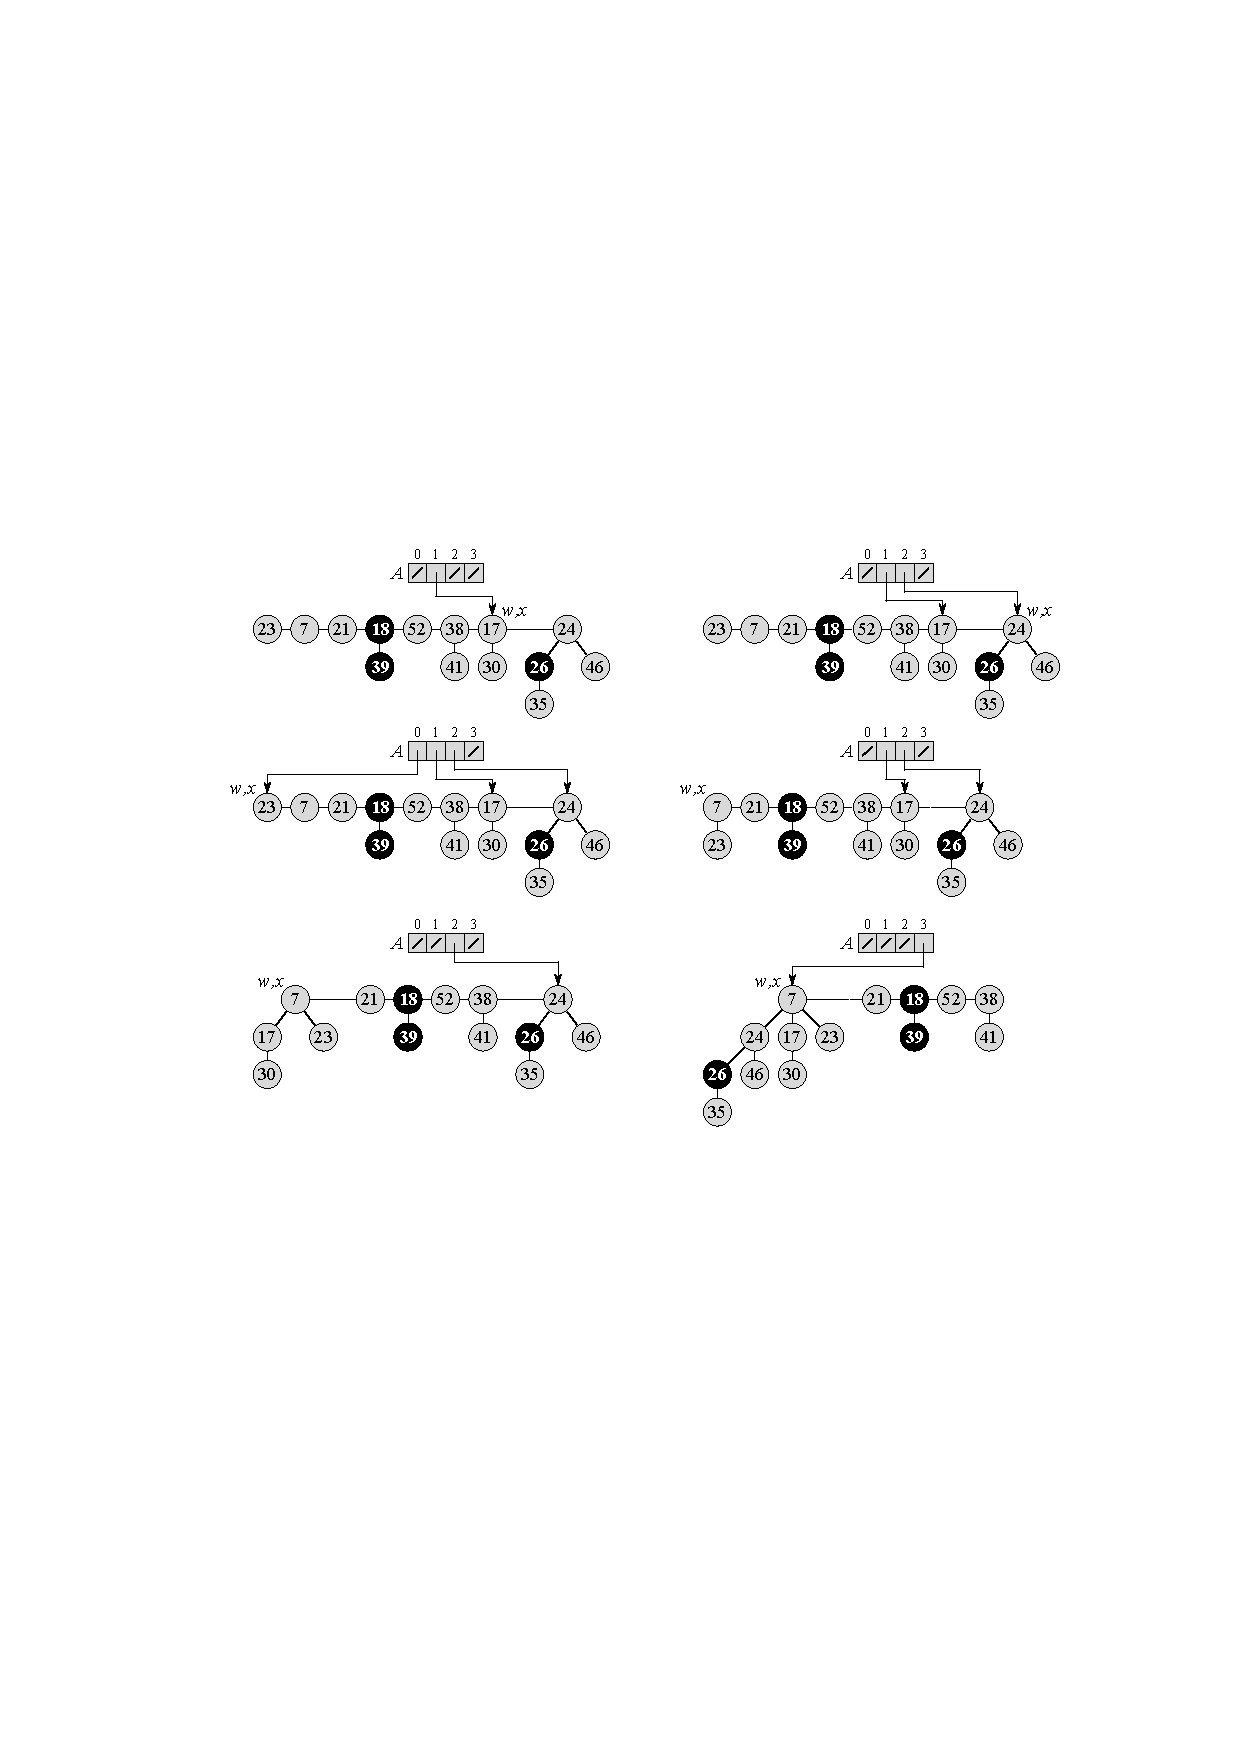
\includegraphics[width=0.75\textwidth]{images/Fibheap2.pdf}
	\caption{A run of \textsc{Consolidate}}
\end{figure}
heaps of same degree then it makes the one with higher key to be the child of the other one. The function \textsc{Fib-Heap-Link} does this process of linking two heaps of same degree.\parinn

Of course in order to allocate array we have to know how to calculate the upper bound for $D(n)$ on the maximum degree. We will show an upper bound of $O(\log n)$ in \autoref{max-degree-bound}.

Now in \textsc{Fib-Extract-Min} in each iteration of the outer for loop or inner while loop it operates on one heap in $F.\emph{rootlist}$. Hence it takes $O(D(n)+\#\text{heaps in $F.\emph{rootlist}$})$ time.


\subsection{Decreasing Key of a Node}
In this section we will show how to decrease a key of a node in a Fibonacci heap in $O(1)$ amortized time. The \textsc{Fib-Decrease-Key} function decreases the key value of the target node then if the min-heap order the node is in is violated then we use the \textsc{Cascading-Cut} function to restore the min-heap property again. These two functions operates like the following:
\begin{center}
	\begin{minipage}{0.45\textwidth}
		\begin{algorithm}[H]
			\caption{\textsc{Fib-Decrease-Key}$(F,x,k)$}
			\DontPrintSemicolon
			\If{$k>x.\emph{key}$}{
				\Return{Error}
			}
			$x.\emph{key}\longleftarrow k$\;
			$y\longleftarrow x.\emph{parent}$\;
			\If{$y\neq None$ and $x.\emph{key}<y.\emph{key}$}{
				\textsc{Cut}$(F,x,y)$\;
				\textsc{Cascading-Cut}$(F,y)$\;
			}
			\If{$k<F.\min.\emph{key}$}{
				$F.\min\longleftarrow x$
			}
		\end{algorithm}
	\end{minipage}\hfill
	\begin{minipage}{0.45\textwidth}
		\begin{algorithm}[H]
			\caption{\textsc{Cascading-Cut}$(F,y)$}
			\DontPrintSemicolon
			% $z\longleftarrow y.\emph{parent}$\;
			\If{$y.\emph{parent}\neq None$}{
				\If{$y.\emph{lost}==0$}{
					$y.\emph{lost}\longleftarrow 1$\;
				}
				\Else{
					\textsc{Cut}$(F,y,y.\emph{parent})$\;
					\textsc{Cascading-Cut}$(F,y.\emph{parent})$
				}
			}
		\end{algorithm}
		\begin{algorithm}[H]
			\caption{\textsc{Cut}$(F,x,y)$}
			\DontPrintSemicolon
			Remove $x$ from $y.\emph{child}$\;
			$y.\emph{degree}\longleftarrow y.\emph{degree}-1$\;
			$F.\emph{rootlist}.\emph{append}(x)$\;
			$x.\emph{parent}\longleftarrow None$, $x.\emph{lost}\longleftarrow 0$\;
		\end{algorithm}
	\end{minipage}
\end{center}
After decreasing the key of the target node if the min-heap order has been violated then we start by cutting the link between $x$ and its parent by adding it to the rootlist. Let $x$ is a node in $F$. At some time $x$ was a root. 
\begin{figure}[h!]
	\centering
	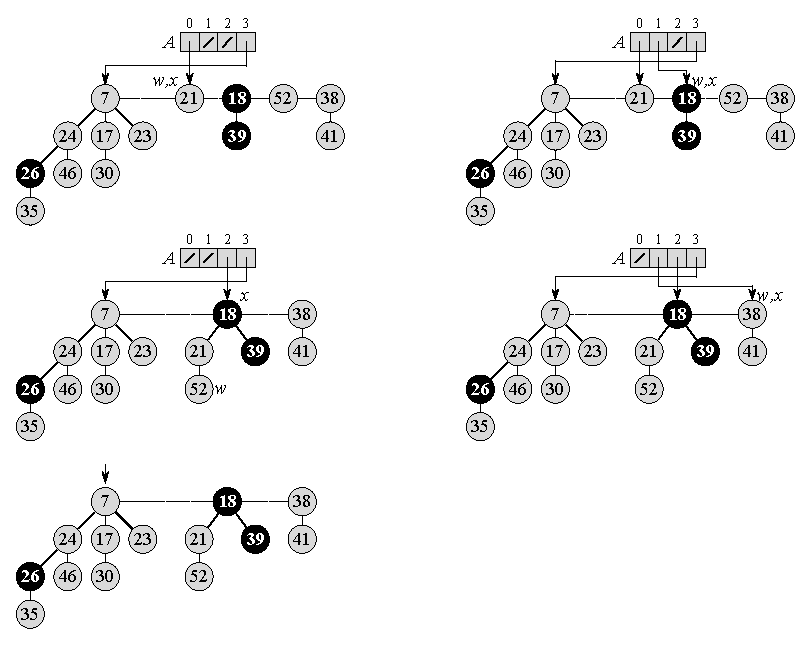
\includegraphics[width=0.7\textwidth]{images/Fibheap3.pdf}
	\caption{A run of \textsc{Cascading-Cut}}
\end{figure}Then $x$ was linked to another node. Suppose at some time two children of $x$ were removed by cuts. As soon as second child has been lost we cut $x$ from its parent and make it a new root. But we are not done yet. Since $x$ might be the second child cut from its parent. So we have to check for its parent. Therefore, we recursively run \textsc{Cascading-Cut} on its parent till we reach the root or cut the first child from a node.

Notice at each run of \textsc{Cascading-Cut} the \emph{lost} bit of a node is getting reset. Therefore, the total time taken by \textsc{Fib-Decrease-Key} is $O(1+\#\text{lost bits reset})$.
\subsection{Bounding the Maximum Degree}\label{max-degree-bound}
To prove that the amortized time of \textsc{Fib-Extract-Min} and \textsc{Fib-Delete} is $O(\log n)$ we must show that upper bound of the maximum degree of any node after \textsc{Consolidate} function is $O(\log n)$. In particular, we will show its $\lt\lfloor \log_{\phi}n\rt\rfloor$ where $\phi$ is the golden ratio.
\begin{lemma}{}{}
	Let $x$ be any node in a Fibonacci heap, and suppose that $x.\emph{degree}=k$. Let $y_1,\dots, y_k$ denote the children of $x$ in the order in which they were linked to $x$ from the earliest to the latest. Then $y_1.\emph{degree}\geq 0$ and $y_i.\emph{degree}\geq i-2$ for $i=2,\dots, k$.
\end{lemma}
\begin{proof}
	Obviously $y_1.\emph{degree}\geq 0$. The only function that adds a child to a node is the function \textsc{Consolidate}. Now for $i\geq 2$, $y_i$ was linked to $x$ when all of $y_1,\dots, y_{i-1}$ were children of $x$, and therefore we must have had $x.\emph{degree}\geq i-1$. Because node $y_i$ is linked to $x$ only if $x\emph{degree}=y_i.\emph{degree}$ we must also have $y_i.\emph{degree}\geq i-1$. Since then node $y_i$ has lost at most one child, since it would have been cut from $x$ by \textsc{Cascading-Cut} if it had lost two children. We conclude that $y_i.\emph{degree}\geq i-2$.
\end{proof}
\begin{lemma}{}{}
	Let $x$ be a node in a Fibonacci heap and let $k=x.\emph{degree}$. Then $$\emph{size}(x)\geq F_{k+2}\geq \phi^k$$
\end{lemma}
\begin{proof}
	We will prove this using induction. For $k=0$, $F_2=1$ so this is obviously true. For $k=1$ there is one child of $x$. Hence, $\emph{size}(x)=2=F_3$. Suppose this is true for $1,\dots, k-1$. Let $y_1,\dots, y_k$ are the children of $x$  in the order in which they were linked to $x$. By the above lemma we have $y_1.\emph{degree}\geq 0$ and $y_i.\emph{degree}\geq i-2$ for all $i=2,\dots, k$. Hence, by Induction hypothesis we have $\emph{size}(y_i)\geq F_{i-2}$ for all $i=2,\dots, k$. Therefore, \[
		\emph{size}(x) \geq 1+\sum\limits_{i=1}^{k}\emph{size}(y_k)\geq 2+\sum\limits_{i=2}^kF_{k}=1+\sum\limits_{i=0}^k F_k=F_{k+2}\geq \phi^k
	\]Hence, we have the lemma.
\end{proof}
\begin{corollary}{}{}
	The maximum degree of any node in \textsc{Consolidate}, $D(n)=O(\log n)$.
\end{corollary}
\subsection{Time Complexity Analysis of Dijkstra}

Now we will calculate the amortized time of Dijkstra algorithm. Before that we will calculate the amortized cost of the data structure. Let in an algorithm  \textsc{Fib-Extract-Min} was called $t$ times. Therefore, total cost of all $t$ many \textsc{Fib-Extract-Min} calls is $O(t\log n+\text{total $\#$heaps created})$. Now heaps are created because of \textsc{Fib-Extract-Min} functions and \textsc{Fib-Decrease-Key} function. We know \textsc{Fib-Extract-Min} were called $t$ times and each time it created $O(\log n)$ heaps. Hence, in total \textsc{Fib-Extract-Min} created $O(t\log n)$ heaps. Therefore, time taken by the $t$ many \textsc{Fib-Extract-Min} calls is $O(t\log n+\#\textsc{Fib-Decrease-Key}\text{ calls})$.

Now suppose in an algorithm $k$ times the function \textsc{Fib-Decrease-Key} function were called. Hence, this takes $O(k+\#\text{total number of \textsc{lost} bits reset})=O(k+\#\text{total number of \textsc{lost} bits rset})$ time. Now the \emph{lost} bits are set only by the \textsc{Fib-Decrease--Key}. Therefore, $\#\text{total number of \textsc{lost} bits rset}=\#\text{\textsc{Fib-Decrese-Key} was called}$. Therefore, the total time taken by all the \textsc{Fib-Decrese-Key} calls is $O(k)$.

Hence, in an algorithm if $t$ times \textsc{Fib-Extract-Min} was called and $k$ times \textsc{Fib-Decrese-Key} was called then total time taken by \textsc{Fib-Extract-Min} is $O(t\log n+k)$ and total time taken by \textsc{Fib-Decrese-Key} is $O(k)$. Therefore, amortized time taken by \textsc{Fib-Extract-Min} is $O(\frac{t}{k}\log n)$ and by \textsc{Fib-Decrese-Key} is $O(1)$.

Now in the Dijkstra algorithm \textsc{Fib-Extract-Min} is called $n$ times and \textsc{Fib-Decrese-Key} is called $O(m)$ times where $n$ is the number of vertices in the graph and $m$ is the number of edges in the graph. Hence, the amortized cost of \textsc{Fib-Extract-Min} is $O(\log n)$ and \textsc{Fib-Decrease-Key} is $O(1)$. Therefore, using Fibonacci heap Dijkstra takes $(n\log n+m)$ time.

\chapter{Kruskal Algorithm with Data Structure}

\section{Kruskal Algorithm}
\begin{center}
\hspace*{4mm}\begin{tikzpicture}[vertex/.style={circle, draw, fill=white, inner sep=2pt}]
\begin{scope}[shift={(-5,0)}]
		\node[vertex] (1) at (0, 0) {};
	\node[vertex] (2) at (1, 1) {};
	\node[vertex] (3) at (1, -1) {};
	\node[vertex] (4) at (2, 0) {};
	\node[vertex] (5) at (4, 0.5) {};
	\node[vertex] (6) at (6, 2) {};
	\node[vertex] (7) at (5, -0.5) {};
	\node[vertex] (8) at (3, -1) {};
	\node[vertex] (9) at (0, -2) {};
	
	%    % Edges with weights (some edges have bends to avoid crossing)
	\draw[shorten >=1pt, shorten <=1pt] (1) -- (2) node[midway, xshift=-1mm,yshift=2mm] {6};
	\draw[shorten >=1pt, shorten <=1pt] (1) -- (3) node[midway, xshift=1mm,yshift=2mm] {3};
	\draw[shorten >=1pt, shorten <=1pt] (2) -- (3) node[midway, right] {14};
	\draw[shorten >=1pt, shorten <=1pt] (2) -- (4) node[midway, above right] {12};
	\draw[shorten >=1pt, shorten <=1pt] (3) -- (4) node[midway, xshift=1mm,yshift=-2mm] {2};
	\draw[shorten >=1pt, shorten <=1pt] (4) -- (5) node[midway, below right] {7};
	\draw[shorten >=1pt, shorten <=1pt] (2) to [bend left=60] (5) node[xshift=-1.5cm, yshift=1.2cm] {15};
	\draw[shorten >=1pt, shorten <=1pt] (5) -- (6) node[midway, above left] {18};
	\draw[shorten >=1pt, shorten <=1pt] (6) -- (7) node[midway, xshift=-3mm, yshift=-1mm] {24};
	\draw[shorten >=1pt, shorten <=1pt] (7) -- (8) node[midway, above left]{16};
	\draw[shorten >=1pt, shorten <=1pt] (3) -- (8) node[midway, below] {5};
	\draw[shorten >=1pt, shorten <=1pt] (3) to [bend right=80, looseness=1.5] (6) node[xshift=-1.5cm, yshift=-4.1cm] {10};
	\draw[shorten >=1pt, shorten <=1pt] (3) -- (9) node[midway, xshift=-1mm,yshift=2mm] {9};
\end{scope}
\draw[ultra thick, -Stealth] (2,0)  -- (4.2,0) node[midway, above] {Kruskal} node[midway, below] {Algorithm};
\begin{scope}[shift={(5,0)}]
	\node[vertex] (1) at (0, 0) {};
	\node[vertex] (2) at (1, 1) {};
	\node[vertex] (3) at (1, -1) {};
	\node[vertex] (4) at (2, 0) {};
	\node[vertex] (5) at (4, 0.5) {};
	\node[vertex] (6) at (6, 2) {};
	\node[vertex] (7) at (5, -0.5) {};
	\node[vertex] (8) at (3, -1) {};
	\node[vertex] (9) at (0, -2) {};
	
	%    % Edges with weights (some edges have bends to avoid crossing)
	\draw[shorten >=1pt, shorten <=1pt, red, thick] (1) -- (2) node[midway, xshift=-1mm,yshift=2mm] {6};
	\draw[shorten >=1pt, shorten <=1pt, red, thick] (1) -- (3) node[midway, xshift=1mm,yshift=2mm] {3};
	\draw[shorten >=1pt, shorten <=1pt] (2) -- (3) node[midway, right] {14};
	\draw[shorten >=1pt, shorten <=1pt] (2) -- (4) node[midway, above right] {12};
	\draw[shorten >=1pt, shorten <=1pt, red, thick] (3) -- (4) node[midway, xshift=1mm,yshift=-2mm] {2};
	\draw[shorten >=1pt, shorten <=1pt, red, thick] (4) -- (5) node[midway, below right] {7};
	\draw[shorten >=1pt, shorten <=1pt] (2) to [bend left=60] (5) node[xshift=-1.5cm, yshift=1.2cm] {15};
	\draw[shorten >=1pt, shorten <=1pt] (5) -- (6) node[midway, above left] {18};
	\draw[shorten >=1pt, shorten <=1pt] (6) -- (7) node[midway, xshift=-3mm, yshift=-1mm] {24};
	\draw[shorten >=1pt, shorten <=1pt, red, thick] (7) -- (8) node[midway, above left]{16};
	\draw[shorten >=1pt, shorten <=1pt, red, thick] (3) -- (8) node[midway, below] {5};
	\draw[shorten >=1pt, shorten <=1pt, red, thick] (3) to [bend right=80, looseness=1.5] (6) node[xshift=-1.5cm, yshift=-4.1cm] {10};
	\draw[shorten >=1pt, shorten <=1pt, red, thick] (3) -- (9) node[midway, xshift=-1mm,yshift=2mm] {9};
\end{scope}
\end{tikzpicture}
\end{center}

\section{Data Structure 1: Array}

\section{Data Structure 2: Left Child Right Siblings Tree}

\section{Data Structure 3: Union Find}
\chapter{Red Black Tree Data Structure}
A red-black tree is a special type of binary search tree with one extra bit of storage per node, its color which can be either red or black. Also, we keep the tree approximately balanced by enforcing some properties on the tree.
\begin{definition}{Perfect Binary Tree}{}
	It is a Binary Tree in which every internal node has exactly two children and all leaves are at the same level.
\end{definition}
\begin{Lemma}{}{}
	Every perfect binary tree with $k$ leaves has $2k-1$  nodes (i.e. $k-1$ internal nodes).
\end{Lemma}
\begin{definition}{Red Black Tree}{}
	\begin{minipage}{0.5\textwidth}
		A red-black tree is a binary tree with the following properties:
		\begin{itemize}
			\item Every internal node is key/NIL node. Every leaf is a ``NIL'' node.
			\item Each node (NIL and key) is colored either red or black.
			\item  Root and NIL nodes are always black.
			\item Any child of a red node is black.
			\item The path from root to any leaf has the same number of black nodes.
		\end{itemize}
	\end{minipage}\hfill
	\begin{minipage}{0.49\textwidth}
		\centering
		\usetikzlibrary{trees,arrows,positioning, calc}
		\begin{tikzpicture}[
				level/.style={sibling distance=30mm/#1},
				level distance=10mm,
				redVertex/.style={draw=red!80!black,fill=red!5!white,circle,minimum size=20pt,inner sep=0pt, text=red!80!black},
				blackVertex/.style={draw,fill=black!10!white,   circle,minimum size=20pt,inner sep=0pt},
				nil/.style={draw,fill=black,rectangle,rounded corners, minimum size=18pt,inner sep=0pt, text=white}]
			\node [blackVertex] (r){29}
			child {
					node[redVertex] {14}
					child [sibling distance=22mm] {
							node[blackVertex] {6}
							child {node [nil] {NIL}}
							child {node [nil] {NIL}}
						}
					child [sibling distance=22mm] {
							node [blackVertex] {24}
							child [sibling distance=15mm] {
									node [redVertex] {18}
									child {node [nil] {NIL}}
									child {node [nil] {NIL}}
								}
							child [sibling distance=15mm] {
									node [redVertex] {26}
									child {node [nil] {NIL}}
									child {node [nil] {NIL}}
								}
						}
				}
			child {
					node[blackVertex] {37}
					child {node [nil] {NIL}}
					child {
							node [redVertex] {66}
							child {node [nil] {NIL}}
							child { node [nil] {NIL}}
						}
				};
		\end{tikzpicture}
		\captionof{figure}{A Red Black Tree}
		\label{fig:red-black-tree}
	\end{minipage}
\end{definition}

We call the number of black nodes on any simple path from  but not including a node $x$ down to a leaf the \emph{black-height} of the node, denoted by $bh(x)$. We generally confine our interest to the internal nodes of a red-black tree, since they hold the key values.
\begin{Lemma}{}{}
	A Red-Black Tree with $n$ internal nodes or key nodes has height at most $O(\log n)$.
\end{Lemma}
\begin{proof}
	We will first show that for any subtree rooted at node $x$ contains at least $2^{bh(x)}-1$ internal nodes. We will show this using induction on the height of the tree. For the base case let height of $x$ is $1$. Then $x$ must be a leaf. Therefore, the subtree rooted at $x$ has at least $bh(x)=1$. Hence, $2^{bh(x)}-1=2^1-1=1$  nodes which is true. For inductive step let $x$ has height greater than $1$, and it is an internal node of the R-B Tree. Now $x$ has two children. Hence, each child has black-height either $bh(x)$ or $bh(x)-1$. By inductive hypothesis, the subtrees rooted at the children of $x$ have at least $2^{bh(x)-1}-1$ internal nodes. Thus, subtree rooted at $x$ has at least $2^{bh(x)-1}-1+2^{bh(x)-1}-1+1=2^{bh(x)}-1$ internal nodes.

	Now if the R-B tree has height $h$. Then any path from the root to a leaf at least half the nodes including the root must be black. So $bh(\emph{root})\geq \frac{h}2$. Thus, $n\geq 2^{\frac{h}2}-1\implies h\leq 2\log(n+1)$. Hence, we have the lemma.
\end{proof}
\nt{
	\begin{minipage}{0.3\textwidth}
		\centering
		\begin{tikzpicture}[
				level distance=8mm,
				vertex/.style={draw,fill=black!10!white,circle,minimum size=15pt,inner sep=0pt},
				nil/.style={draw,fill=black,rectangle,rounded corners, minimum size=18pt,inner sep=0pt, text=white}
			]
			\node[vertex] (a) {}
			child { node [nil] {NIL} }
			child {
					node [vertex] (b) {}
					child { node [nil] {NIL} }
					child {
							node [vertex] (c) {}
							child { node [nil] {NIL} }
							child { node [nil] {NIL} }
						}
				};
		\end{tikzpicture}
	\end{minipage}\hfill
	\begin{minipage}{0.69\textwidth}
		Not all trees can be colored in a way that satisfies the properties of a red-black tree. Consider the following tree:\parinn

		In this example the root has to be black. The other two internal nodes can not be black since otherwise the path from the leaf of the root to root has only 2 black nodes but in the path from bottom most leaf to root will have 3. Then those two internal nodes has to be red. But that violates the property that a red node can not have a red child. Hence, this tree can not be colored in a way that satisfies the properties of a red-black tree.
	\end{minipage}
}

Since by the lemma the R-B tree has height at most $O(\log n)$ and it is a binary search tree we can perform search of a node using \textsc{Find} in $O(\log n)$ time. So now we will focus on the insertion and deletion operations in a red-black tree.  To insert or delete a node in a red-black tree we will do  rotations to balance the tree again. So first we will visit rotations.
\section{Rotation}
A rotation is a local operation that changes the structure of a binary tree without violating the binary search tree property. There are two types of rotations: left rotation and right rotation.

When we do a left rotation on a node we assume that its right child is not NIL. The left rotation ``pivots'' around the link from the node to its right child and makes the right child the new root of the subtree with the node as its left child.  Similarly, we can explain the right rotation. The rotations behave like the following:

\begin{figure}[!h]
	\centering
	\begin{tikzpicture}[
			every node/.style={align=center, line width=0.15mm},
			level 1/.style={level distance=1cm, sibling distance=1.5cm},  % Adjusted distance for level 1
			level 2/.style={sibling distance=1.5cm},   % Adjusted distance for level 2
			square/.style={draw, shape=rectangle, minimum width=0.5cm, minimum height=0.5cm, inner sep=0pt, text width=0.5cm, text centered},
			circle/.style={draw, shape=circle, minimum width=0.5cm, minimum height=0.5cm, inner sep=0pt, text width=0.5cm, text centered},
			filled/.style={fill=white, , draw, line width=0.12mm},  % Style for filled nodes
			every edge/.style = {draw, latex'-latex' , line width=0.3mm, dotted,},
			parentarrow/.style={line width=0.12mm},  % Style for arrows from nodes to children
		]

		% Leftmost tree
		\node (A0) {}
		child{
				node[circle] (A1) {$u$}
				child {node[circle] (B1) {$v$}
						child {node[square] (D1) {$\alpha$} edge from parent[parentarrow]}
						child {node[square] (E1) {$\beta$} }
						edge from parent[parentarrow]
					}
				child {node[square,filled] (C1) {$\gm$} edge from parent[parentarrow]}
			}
		child [missing] { node (A5) {} };

		% Right tree
		\begin{scope}[shift={(6,0)}]
			\node (AA0) {}
			child{
					node[circle] (A2) {$v$}
					child {node[square,filled] (C2) {$\alpha$} edge from parent[parentarrow]}
					child {node[circle] (B2) {$u$}
							child {node[square] (D2) {$\beta$} edge from parent[parentarrow]}
							child {node[square] (E2) {$\gm$} }
							edge from parent[parentarrow]
						}
				}
			child [missing] { node (AA5) {} };

		\end{scope}

		\draw[thick, -left to] ($(C1)+(1,0.05)$) -- node[midway, above] {Right Rotate} ($(C2)+(-1,0.05)$);
		\draw[thick, -left to] ($(C2)+(-1,-0.05)$) -- node[midway, below] {Left Rotate}($(C1)+(1,-0.05)$)  ;
	\end{tikzpicture}
	\caption{Left and Right rotate about $u-v$}
\end{figure}\parinf

\begin{minipage}{0.46\textwidth}
	\begin{algorithm}[H]
		\caption{\textsc{Left-Rotate}$({T,x})$}
		\DontPrintSemicolon
		$y\longleftarrow x.\emph{right}$\;
		$x.\emph{right}\longleftarrow y.\emph{left}$\;
		\If{$y.\emph{left}\neq \emph{NIL}$}{
			$y.\emph{left}.\emph{parent}\longleftarrow x$\;
		}
		$y.\emph{parent}\longleftarrow x.\emph{parent}$\;
		\If{$x.\emph{parent}==\emph{NIL}$}{
			$T.\emph{root}\longleftarrow y$\;
		}
		\ElseIf{$x== x.\emph{parent}.\emph{left}$}{
			$x.\emph{parent}.\emph{left}\longleftarrow y$\;
		}
		\Else{
			$x.\emph{parent}.\emph{right}\longleftarrow y$\;
		}
		$y.\emph{left}\longleftarrow x$\;
		$x.\emph{parent}\longleftarrow y$
	\end{algorithm}
\end{minipage}\hfill
\begin{minipage}{0.46\textwidth}
	\begin{algorithm}[H]
		\caption{\textsc{Right-Rotate}$({T,x})$}
		\DontPrintSemicolon
		$y\longleftarrow x.\emph{left}$\;
		$x.\emph{left}\longleftarrow y.\emph{right}$\;
		\If{$y.\emph{right}\neq \emph{NIL}$}{
			$y.\emph{right}.\emph{parent}\longleftarrow x$\;
		}
		$y.\emph{parent}\longleftarrow x.\emph{parent}$\;
		\If{$x.\emph{parent}==\emph{NIL}$}{
			$T.\emph{root}\longleftarrow y$\;
		}
		\ElseIf{$x== x.\emph{parent}.\emph{left}$}{
			$x.\emph{parent}.\emph{left}\longleftarrow y$\;
		}
		\Else{
			$x.\emph{parent}.\emph{right}\longleftarrow y$\;
		}
		$y.\emph{right}\longleftarrow x$\;
		$x.\emph{parent}\longleftarrow y$
	\end{algorithm}
\end{minipage}\parinn

Both \textsc{Left-Rotate} and \textsc{Right-Rotate} take $O(1)$ time. Only some constantly many pointers are changed by rotation all other attributes in a node remain the same.
\section{Insertion}
We will now describe how to insert a node in a red-black tree in $O(\log n)$ time. We will insert the node in the tree in place of a leaf replacing a NIL node. After that we will color the node red. Let the node added is $v$. We define the attribute \emph{uncle} which is basically sibling of the parent. Now two cases can happen:
\begin{enumerate}[label=Case \Roman*:, leftmargin=*]
	\item $v.\emph{uncle}.color=$ Red: Then $v.\emph{parent}.\emph{parent}$  is black. In this case we can recolor $v.\emph{parent}.\emph{parent}$ to red and both $v.\emph{parent}$ and $v.\emph{uncle}$ to be black. This will preserve the number of black nodes in any simple path from root to any leaf.
	      \begin{figure}[!h]
		      \centering
		      \begin{tikzpicture}[
				      every node/.style={align=center, line width=0.15mm},
				      level 1/.style={level distance=1.2cm, sibling distance=1.8cm},  % Adjusted distance for level 1
				      level 2/.style={sibling distance=1.8cm},   % Adjusted distance for level 2
				      redVertex/.style={draw, shape=circle, minimum width=1.1cm, minimum height=0.5cm, inner sep=0pt, text width=1cm, text centered, text=red!75!black, color=red},
				      blackVertex/.style={draw, shape=circle, minimum width=1.1cm, minimum height=0.5cm, inner sep=0pt, text width=1cm, text centered},
				      every edge/.style = {draw, latex'-latex' , line width=0.3mm, dotted,},
				      Rparentarrow/.style={line width=0.12mm, color=red},  % Style for arrows from nodes to children
				      parentarrow/.style={line width=0.12mm}
			      ]

			      % Leftmost tree
			      \node (AA0) {}
			      child{
					      node[blackVertex] (A2) {$v.p.p$}
					      child {node[redVertex] (B2) {$v.p$}
							      child {node[blackVertex] (D2) {$v.s$} edge from parent[parentarrow]}
							      child {node[redVertex] (E2) {$v$} }
							      edge from parent[parentarrow]
						      }
					      child {node[redVertex] (C2) {$v.u$} edge from parent[parentarrow]}
				      }
			      child [missing] { node (AA5) {} };
			      % Right tree
			      \begin{scope}[shift={(6,0)}]
				      \node (A0) {}
				      child{
						      node[redVertex] (A1) {$v.p.p$}
						      child {node[blackVertex] (B1) {$v.p$}
								      child {node[blackVertex] (D1) {$v.s$} edge from parent[parentarrow]}
								      child {node[redVertex] (E1) {$v$} }
								      edge from parent[parentarrow]
							      }
						      child {node[blackVertex] (C1) {$v.u$} edge from parent[parentarrow]}
					      }
				      child [missing] { node (A5) {} };
			      \end{scope}

			      \draw[thick, -latex] ($(C2)+(1,0.05)$) -- node[midway, above] {Recolor} ($(B1)+(-1,0.05)$);
		      \end{tikzpicture}
	      \end{figure}
	      Now the color of $v.\emph{parent}.\emph{parent}$ is red, and therefore we iterate the same process on $v.\emph{parent}.\emph{parent}$.
	\item $v.\emph{uncle}.\emph{color}=$ Black: In this case we need two rotations. First we do a left rotation on $v.\emph{parent}$. After that we do a right rotation on $v.\emph{parent}.\emph{parent}$. After the rotations, we recolor the nodes.
	      \begin{figure}[!h]
		      \centering
		      \begin{tikzpicture}[
				      every node/.style={align=center, line width=0.15mm},
				      level 1/.style={level distance=1.2cm, sibling distance=1.8cm},  % Adjusted distance for level 1
				      level 2/.style={sibling distance=1.8cm},   % Adjusted distance for level 2
				      redVertex/.style={draw, shape=circle, minimum width=1.1cm, minimum height=0.5cm, inner sep=0pt, text width=1cm, text centered, text=red!75!black, color=red},
				      blackVertex/.style={draw, shape=circle, minimum width=1.1cm, minimum height=0.5cm, inner sep=0pt, text width=1cm, text centered},
				      every edge/.style = {draw, latex'-latex' , line width=1mm},
				      Rparentarrow/.style={line width=0.12mm, color=red},  % Style for arrows from nodes to children
				      parentarrow/.style={line width=0.12mm}
			      ]

			      % Leftmost tree
			      \begin{scope}[shift={(1,0)}]
				      \node (AA0) {}
				      child{
						      node[blackVertex] (A2) {$v.p.p$}
						      child {node[redVertex] (B2) {$v.p$}
								      child {node[blackVertex] (D2) {$v.s$} edge from parent[parentarrow]}
								      child {
										      node[redVertex] (E2) {$v$}
										      child { node[blackVertex] (F1) {$v.s$} edge from parent[parentarrow] }
										      child { node[blackVertex] (G1) {$v.l$} edge from parent[parentarrow] }
									      }
								      edge from parent[parentarrow]
							      }
						      child {node[blackVertex] (C2) {$v.u$} edge from parent[parentarrow]}
					      }
				      child [missing] { node (AA5) {} };
			      \end{scope}
			      % Right tree
			      \begin{scope}[shift={(8,0)}]
				      \node (A0) {}
				      child{
						      node[blackVertex] (A1) {$v.p.p$}
						      child {node[redVertex] (B1) {$v$}
								      child {
										      node[redVertex] (D1) {$v.p$} edge from parent[parentarrow]
										      child { node[blackVertex] (F1) {$v.s$} edge from parent[parentarrow] }
										      child { node[blackVertex] (G1) {$v.l$} edge from parent[parentarrow] }
									      }
								      child {node[blackVertex] (E1) {$v.r$} }
								      edge from parent[parentarrow]
							      }
						      child {node[blackVertex] (C1) {$v.u$} edge from parent[parentarrow]}
					      }
				      child [missing] { node (A5) {} };
			      \end{scope}
			      \begin{scope}[shift={(8,-7.5)}]
				      \node (AAA0) {}
				      child[sibling distance=2.5cm]{
						      node[redVertex] (A3) {$v$}
						      child[sibling distance=2.5cm] {node[redVertex] (B3) {$v.p$}
								      child[sibling distance=1.2cm] {node[blackVertex] (D3) {$v.s$} edge from parent[parentarrow]}
								      child[sibling distance=1.2cm] {node[blackVertex] (E3) {$v.l$} }
								      edge from parent[parentarrow]
							      }
						      child[sibling distance=2.5cm] {
								      node[blackVertex] (C3) {$v.p.p$} edge from parent[parentarrow]
								      child[sibling distance=1.2cm] { node[blackVertex] (F3) {$v.r$} edge from parent[parentarrow] }
								      child[sibling distance=1.2cm] { node[blackVertex] (G3) {$v.u$} edge from parent[parentarrow] }
							      }
					      }
				      child [sibling distance=2.5cm,missing] { node (AAA5) {} };
			      \end{scope}
			      \begin{scope}[shift={(1,-7.5)}]
				      \node (AAAA0) {}
				      child[sibling distance=2.5cm]{
						      node[blackVertex] (A4) {$v$}
						      child[sibling distance=2.5cm] {node[redVertex] (B4) {$v.p$}
								      child[sibling distance=1.2cm] {node[blackVertex] (D4) {$v.s$} edge from parent[parentarrow]}
								      child[sibling distance=1.2cm] {node[blackVertex] (E4) {$v.l$} }
								      edge from parent[parentarrow]
							      }
						      child[sibling distance=2.5cm] {
								      node[redVertex] (C4) {$v.p.p$} edge from parent[parentarrow]
								      child[sibling distance=1.2cm] { node[blackVertex] (F4) {$v.r$} edge from parent[parentarrow] }
								      child[sibling distance=1.2cm] { node[blackVertex] (G4) {$v.u$} edge from parent[parentarrow] }
							      }
					      }
				      child [sibling distance=2.5cm,missing] { node (AAAA5) {} };
			      \end{scope}
			      \draw[thick, -latex] ($(C2)+(1,0.05)$) -- node[midway, above] {\textsc{Left-Rotate}$(v.p)$} ($(B1)+(-1,0.05)$);
			      \draw($(C1)+(1,0)$) edge [bend left=60, thick, -latex]  node[midway, right, rotate=-90, xshift=-2cm, yshift=0.3cm] {\textsc{Right-Rotate}$(v.p.p)$} ($(C3)+(1,0)$);
			      \draw[thick, -latex] ($(B3)+(-1,0.05)$) -- node[midway, above] {Recolor} ($(C4)+(1,0.05)$);
		      \end{tikzpicture}
	      \end{figure}
	      The color of $v.\emph{parent}.\emph{parent}$  and the color of $v.\emph{parent}$ will be red. The color of $v$ will be recolored black. This will preserve the number of black nodes in any simple path from root to any leaf. And this case now stabilizes the tree, and we can stop the process.
\end{enumerate}
So analyzing the insertion process we can insert a node in a red-black tree and using the two cases we can recolor the nodes the balance the tree.\parinf

\begin{minipage}{0.46\textwidth}
	\begin{algorithm}[H]
		\caption{\textsc{RB-Insert}$(T,v)$}
		\DontPrintSemicolon
		$y\longleftarrow \emph{NIL}$, $x\longleftarrow T.\emph{root}$\;
		\While{$x\neq \emph{NIL}$}{
			$y\longleftarrow x$\;
			\If{$v.\emph{key}<x.\emph{key}$}{
				$x\longleftarrow x.\emph{left}$\;
			}
			\Else{
				$x\longleftarrow x.\emph{right}$\;
			}
		}
		$v.\emph{parent}\longleftarrow y$\;
		\If{$y==\emph{NIL}$}{
			$T.\emph{root}\longleftarrow v$\;
		}
		\ElseIf{$v.\emph{key}<y.\emph{key}$}{
			$y.\emph{left}\longleftarrow v$\;
		}
		\Else{
			$y.\emph{right}\longleftarrow v$\;
		}
		$v.\emph{left}\longleftarrow \emph{NIL}$,
		$v.\emph{right}\longleftarrow \emph{NIL}$, $v.\emph{color}\longleftarrow RED$\;
		\textsc{RB-Insert-Fixup}$(T,v)$\;
	\end{algorithm}
\end{minipage}\hfill
\begin{minipage}{0.5\textwidth}
	\begin{algorithm}[H]
		\SetKwComment{Comment}{// }{}
		\caption{\textsc{RB-Insert-Fixup}$(T,v)$}
		\DontPrintSemicolon
		\While{$v.\emph{parent}.\emph{color}==RED$}{
			\If{$v.\emph{parent}.\emph{parent}==NIL$}{$v.\emph{parent}.\emph{color}\longleftarrow BLACK$\;Break\;}
			$vu\longleftarrow v.\emph{parent}.\emph{parent}.\emph{right}$\Comment*{Uncle}
			$vpp\longleftarrow v.\emph{parent}.\emph{parent}$\;
			\If{$vu.\emph{color}==RED$}{
				$v.\emph{parent}.\emph{color}\longleftarrow BLACK$\Comment*{Case I}
				$vu.\emph{color}\longleftarrow BLACK$\;
				$vpp.\emph{color}\longleftarrow RED$\;
				$v\longleftarrow vpp$
			}
			\Else{
				\textsc{Left-Rotate}$(T,v.\emph{parent})$\Comment*{Case II}
				\textsc{Right-Rotate}$(T,vpp)$\;
				$v.\emph{color}\longleftarrow BLACK$\;
				$vpp.\emph{color}\longleftarrow RED$\;
				Break
			}
		}
	\end{algorithm}
\end{minipage}
\parinn

Since the Case I can happen at most $O(\log n)$ times as each use of Case I increase the height by $2$, the while loop can run at most $O(\log n)$ times. Therefore, insertion of a node in a red-black tree takes $O(\log n)$ time.
\section{Deletion}
Like insertion, deletion of a node involves recoloring and rotations to maintain the properties of a red-black tree. Here we will use a notion of double-black color. In the deletion we will use something called in-order traversal of the binary tree and use successor and predecessor of a node in the traversal. \begin{Definition}{In-Order Traversal}{}
	In-Order Traversal of a binary tree is a traversal where:\begin{itemize}
		\item Recursively traverse the current node left subtree.
		\item Visit the current node.
		\item Recursively traverse the current node right subtree.
	\end{itemize}
	The in-order \emph{successor} (\emph{predecessor}) of a node is the next (previous) node in the in-order traversal of the tree.
\end{Definition}
\begin{observation}
	For any node $x$ the in-order successor of $x$ is the leftmost node in the right subtree of $x$. Similarly, the in-order predecessor of $x$ is the rightmost node in the left subtree of $x$.
\end{observation}
To delete a node $x$ we will replace its \emph{key} by the key of its in-order successor or predecessor (say $y$) and then delete $y$ i.e. after replacing the key of $x$ by the key of $y$, it will still have the color of $x.\emph{color}$. We replace with in-order successor unless $x$ has no right child. In that case we replace with in-order predecessor. If $x$ has no children then we have $y=x$.
\nt{$y$ is either a non-NIL leaf or has exactly one child.}

\begin{enumerate}
	\item $y$ has a child then child must be colored red since otherwise the NIL child of $y$ and any NIL node in the subtree rooted at child of $y$ will have different black-height. Therefore, $y$ must be colored black. Hence, we replace $y$ by its child and color it black.
	\item $y$ is a non-NIL leaf and its colored red. Then we can simply remove $y$ from the tree.
\end{enumerate}
So the only case remained to analyze is when $y$ is a non-NIL leaf and colored black. Now the situation is complicated since removing $y$ would create black-height imbalance in the tree.
\begin{observation}
	If $y.\emph{color}$ is black then $y$ must have a sibling since otherwise sibling of $y$ is NIL. Then that NIL node and any NIL node in the subtree rooted at $y$ will have different black-height.
\end{observation}
So we replace $y$ with a NIL node and color it \emph{double-black} which  will be counted has $2$ black nodes to maintain the black-height. Now we will resolve the double-black color by rotation, recoloring or pushing up the double-black color. We will use the following pointers \begin{itemize}
	\item $y.\emph{sibling}$ to denote the sibling of $y$.
	\item $y.\emph{left-nephew}$ and  $y.\emph{right-nephew}$ to denote the left and right child of $y.\emph{sibling}$.
\end{itemize} We will use the following cases to resolve the double-black color:
\begin{enumerate}[label=Case \Roman*:, leftmargin=*]
	\item  $y.\emph{sibling},y.\emph{parent},y.\emph{left-nephew},y.\emph{right-nephew}$ are all Black. In this case we can make $y.\emph{parent}$ the double black instead of $y$ and recolor the $y$ has black node and sibling of $y$ red color.
	      \begin{figure}[!h]
		      \centering
		      \begin{tikzpicture}[level distance=1cm,
				      every node/.style={align=center, line width=0.15mm},
				      level 1/.style={sibling distance=1.5cm},
				      level 2/.style={sibling distance=1.5cm},
				      redVertex/.style={
						      draw, shape=circle,
						      minimum width=0.9cm, minimum height=0.5cm,
						      inner sep=0pt, text width=0.5cm, text centered,
						      text=red!75!black, color=red
					      },
				      blackVertex/.style={
						      draw, shape=circle,
						      minimum width=0.9cm, minimum height=0.5cm,
						      inner sep=0pt, text width=0.5cm, text centered
					      },
				      doubleBlackVertex/.style={
						      draw, double, shape=circle,
						      minimum width=0.9cm, minimum height=0.5cm,
						      inner sep=0pt, text width=0.5cm, text centered
					      },
				      every edge/.style = {draw, latex'-latex', line width=0.3mm, dotted},
				      parentarrow/.style={line width=0.12mm}
			      ]

			      % Leftmost tree
			      \node (AA0) {}
			      child{
					      node[blackVertex] (A2) {$y.p$}
					      child {node[doubleBlackVertex] (B2) {$y$}}
					      child {
							      node[blackVertex] (C2) {$y.s$} edge from parent[parentarrow]
							      child {node[blackVertex] (D2) {$y.ln$} edge from parent[parentarrow]}
							      child {node[blackVertex] (E2) {$y.rn$} }
							      edge from parent[parentarrow]
						      }
				      }
			      child [missing] { node (AA5) {} };
			      % Right tree
			      \begin{scope}[shift={(6,0)}]
				      \node (A0) {}
				      child{
						      node[doubleBlackVertex] (A1) {$y.p$}
						      child {node[blackVertex] (B1) {$y$}}
						      child {
								      node[redVertex] (C1) {$y.s$} edge from parent[parentarrow]
								      child {node[blackVertex] (D1) {$y.ln$} edge from parent[parentarrow]}
								      child {node[blackVertex] (E1) {$y.rn$} }
								      edge from parent[parentarrow]
							      }
					      }
				      child [missing] { node (A5) {} };
			      \end{scope}

			      \draw[thick, -latex] ($(C2)+(1,0.05)$) -- node[midway, above] {Recolor} ($(B1)+(-1,0.05)$);
		      \end{tikzpicture}
	      \end{figure}
	\item $y.\emph{sibling},y.\emph{left-nephew},y.\emph{right-nephew}$ are Black \& $y.\emph{parent}$ is Red. Here we recolor $y.\emph{parent}$ to black and $y.\emph{sibling}$ to red. This will preserve the number of black nodes in any  path from root to any leaf. So we stop.
	\begin{figure}[!h]
		      \centering
		      \begin{tikzpicture}[level distance=1cm,
				      every node/.style={align=center, line width=0.15mm},
				      level 1/.style={sibling distance=1.5cm},
				      level 2/.style={sibling distance=1.5cm},
				      redVertex/.style={
						      draw, shape=circle,
						      minimum width=0.9cm, minimum height=0.5cm,
						      inner sep=0pt, text width=0.5cm, text centered,
						      text=red!75!black, color=red
					      },
				      blackVertex/.style={
						      draw, shape=circle,
						      minimum width=0.9cm, minimum height=0.5cm,
						      inner sep=0pt, text width=0.5cm, text centered
					      },
				      doubleBlackVertex/.style={
						      draw, double, shape=circle,
						      minimum width=0.9cm, minimum height=0.5cm,
						      inner sep=0pt, text width=0.5cm, text centered
					      },
				      every edge/.style = {draw, latex'-latex', line width=0.3mm, dotted},
				      parentarrow/.style={line width=0.12mm}
			      ]

			      % Leftmost tree
			      \node (AA0) {}
			      child{
					      node[redVertex] (A2) {$y.p$}
					      child {node[doubleBlackVertex] (B2) {$y$}}
					      child {
							      node[blackVertex] (C2) {$y.s$} edge from parent[parentarrow]
							      child {node[blackVertex] (D2) {$y.ln$} edge from parent[parentarrow]}
							      child {node[blackVertex] (E2) {$y.rn$} }
							      edge from parent[parentarrow]
						      }
				      }
			      child [missing] { node (AA5) {} };
			      % Right tree
			      \begin{scope}[shift={(6,0)}]
				      \node (A0) {}
				      child{
						      node[blackVertex] (A1) {$y.p$}
						      child {node[blackVertex] (B1) {$y$}}
						      child {
								      node[redVertex] (C1) {$y.s$} edge from parent[parentarrow]
								      child {node[blackVertex] (D1) {$y.ln$} edge from parent[parentarrow]}
								      child {node[blackVertex] (E1) {$y.rn$} }
								      edge from parent[parentarrow]
							      }
					      }
				      child [missing] { node (A5) {} };
			      \end{scope}

			      \draw[thick, -latex] ($(C2)+(1,0.05)$) -- node[midway, above] {Recolor} ($(B1)+(-1,0.05)$);
		      \end{tikzpicture}
	      \end{figure}
	\item $y.\emph{sibling}$ is Black and $y.\emph{right-nephew}$ is Red. Then we do a \textsc{Left-Rotate} on $y.\emph{parent}$. Then we recolor
	      \begin{figure}[!h]
		      \centering
		      \begin{tikzpicture}[level distance=1cm, sibling distance=1.5cm,
				      every node/.style={align=center, line width=0.15mm},
				      redVertex/.style={
						      draw, shape=circle,
						      minimum width=0.9cm, minimum height=0.5cm,
						      inner sep=0pt, text width=0.5cm, text centered,
						      text=red!75!black, color=red
					      },
				      blackVertex/.style={
						      draw, shape=circle,
						      minimum width=0.9cm, minimum height=0.5cm,
						      inner sep=0pt, text width=0.5cm, text centered
					      },
				      doubleBlackVertex/.style={
						      draw, double, shape=circle,
						      minimum width=0.9cm, minimum height=0.5cm,
						      inner sep=0pt, text width=0.5cm, text centered
					      },
				      halfBorderVertex/.style={
						      circle,
						      minimum width=0.9cm,
						      inner sep=0pt,
						      text width=0.5cm,
						      text centered,
						      path picture={
								      \draw[black, line width=0.3mm]
								      (path picture bounding box.center) ++(90:0.45cm) arc[start angle=90, end angle=270, radius=0.45cm];
								      \draw[red, line width=0.3mm]
								      (path picture bounding box.center) ++(270:0.45cm) arc[start angle=270, end angle=450, radius=0.45cm];
							      }
					      },
				      parentarrow/.style={line width=0.12mm}
			      ]

			      % Leftmost tree
			      \node (AA0) {}
			      child{
					      node[halfBorderVertex] (A2) {$y.p$}
					      child {node[doubleBlackVertex] (B2) {$y$}}
					      child {
							      node[blackVertex] (C2) {$y.s$} edge from parent[parentarrow]
							      child {node[halfBorderVertex] (D2) {$y.ln$} edge from parent[parentarrow]}
							      child {node[redVertex] (E2) {$y.rn$} }
							      edge from parent[parentarrow]
						      }
				      }
			      child [missing] { node (AA5) {} };
			      % Right tree
			      \begin{scope}[shift={(6,0)}]
				      \node (A0) {}
				      child{
						      node[blackVertex] (A1) {$y.s$}
						      child {
								      node[halfBorderVertex] (B1) {$y.p$}
								      child {node[doubleBlackVertex] (D1) {$y$} edge from parent[parentarrow]}
								      child {node[halfBorderVertex] (E1) {$y.ln$} }
								      edge from parent[parentarrow]
							      }
						      child {node[redVertex] (C1) {$y.rn$} edge from parent[parentarrow]}
					      }
				      child [missing] { node (A5) {} };
			      \end{scope}

			      \begin{scope}[shift={(12,0)}]
				      \node (AAA0) {}
				      child{
						      node[halfBorderVertex] (A3) {$y.s$}
						      child {
								      node[blackVertex] (B3) {$y.p$}
								      child {node[blackVertex] (D3) {$y$} edge from parent[parentarrow]}
								      child {node[halfBorderVertex] (E3) {$y.ln$} }
								      edge from parent[parentarrow]
							      }
						      child {node[blackVertex] (C3) {$y.rn$} edge from parent[parentarrow]}
					      }
				      child [missing] { node (AAA5) {} };
			      \end{scope}

			      \draw[thick, -latex] ($(C2)+(0.8,0.05)$) -- node[midway, above] {\textsc{Left-Rotate}$(y.p)$} ($(B1)+(-0.8,0.05)$);
			      \draw[thick, -latex] ($(C1)+(0.8,0.05)$) -- node[midway, above] {Recolor} ($(B3)+(-0.8,0.05)$);
			      \draw[thick, dashed,latex-latex] (E1) edge [bend right=30, shorten <=1mm, shorten >=1mm] node[midway, below] {Same color} (E3);
			      \draw[thick, dashed, latex-latex]
			      (B1) edge [
					      out=100,          % angle leaving B1
					      in=150,          % angle entering E3
					      looseness=1,   % (optional) controls curvature
					      shorten <=1mm,
					      shorten >=1mm
				      ]
			      node[midway, above] {Color same as $y.\emph{parent.color}$}
			      (A3);
		      \end{tikzpicture}
	      \end{figure}  $y.\emph{sibling}$ to the same color as $y.\emph{parent}$. And we recolor $y.\emph{parent}$ to black,  $y.\emph{right-nephew}$ to red and $y$ to black. And now we stop.
	\item $y.\emph{sibling},y.\emph{right-nephew}$ are Black \& $y.\emph{left-nephew}$ is Red. Therefore, both the children of $y.\emph{left-nephew}$ have color black. Here we first do a \textsc{Right-Rotate} on $y.\emph{sibling}$.
	      \begin{figure}[!h]
		      \centering
		      \begin{tikzpicture}[level distance=1.2cm, sibling distance=1.5cm,
				      redVertex/.style={
						      draw, shape=circle,
						      minimum width=1.1cm, minimum height=0.5cm,
						      inner sep=0pt, text width=1cm, text centered,
						      text=red!75!black, color=red
					      },
				      blackVertex/.style={
						      draw, shape=circle,
						      minimum width=1.1cm, minimum height=0.5cm,
						      inner sep=0pt, text width=1cm, text centered
					      },
				      doubleBlackVertex/.style={
						      draw, double, shape=circle,
						      minimum width=1.1cm, minimum height=0.5cm,
						      inner sep=0pt, text width=1cm, text centered
					      },
				      halfBorderVertex/.style={
						      circle,
						      minimum width=1.1cm,
						      inner sep=0pt,
						      text width=1cm,
						      text centered,
						      path picture={
								      \draw[black, line width=0.3mm]
								      (path picture bounding box.center) ++(90:0.55cm) arc[start angle=90, end angle=270, radius=0.55cm];
								      \draw[red, line width=0.3mm]
								      (path picture bounding box.center) ++(270:0.55cm) arc[start angle=270, end angle=450, radius=0.55cm];
							      }
					      },
				      parentarrow/.style={line width=0.12mm}
			      ]

			      % Leftmost tree
			      \node (AA0) {}
			      child{
					      node[halfBorderVertex] (A2) {$y.p$}
					      child {node[doubleBlackVertex] (B2) {$y$}}
					      child {
							      node[blackVertex] (C2) {$y.s$} edge from parent[parentarrow]
							      child {
									      node[redVertex] (D2) {$y.ln$} edge from parent[parentarrow]
									      child { node[blackVertex] (F2) {$y.ln.l$} }
									      child { node[blackVertex] (G2) {$y.ln.r$} }
								      }
							      child {node[blackVertex] (E2) {$y.rn$} }
							      edge from parent[parentarrow]
						      }
				      }
			      child [missing] { node (AA5) {} };
			      % Right tree
			      \begin{scope}[shift={(6,0)}]
				      \node (A0) {}
				      child{
						      node[halfBorderVertex] (A1) {$y.p$}
						      child {node[doubleBlackVertex] (B1) {$y$}}
						      child {
								      node[redVertex] (C1) {$y.ln$} edge from parent[parentarrow]
								      child {										      node[blackVertex] (D1) {$y.ln.l$} edge from parent[parentarrow]									      }
								      child {
										      node[blackVertex] (E1) {$y.s$}
										      child { node[blackVertex] (F1) {$y.ln.r$} }
										      child { node[blackVertex] (G1) {$y.rn$} }
									      }
								      edge from parent[parentarrow]
							      }
					      }
				      child [missing] { node (A5) {} };
			      \end{scope}

			      \begin{scope}[shift={(12,0)}]
				      \node (AAA0) {}
				      child{
						      node[halfBorderVertex] (A3) {$y.p$}
						      child {node[doubleBlackVertex] (B3) {$y$}}
						      child {
								      node[blackVertex] (C3) {$y.ln$} edge from parent[parentarrow]
								      child {										      node[blackVertex] (D3) {$y.ln.l$} edge from parent[parentarrow]									      }
								      child {
										      node[redVertex] (E3) {$y.s$}
										      child { node[blackVertex] (F3) {$y.ln.r$} }
										      child { node[blackVertex] (G3) {$y.rn$} }
									      }
								      edge from parent[parentarrow]
							      }
					      }
				      child [missing] { node (AAA5) {} };
			      \end{scope}

			      \draw[thick, -latex] ($(C2)+(0.8,0.05)$) -- node[midway, above] {\textsc{Right-Rotate}$(y.s)$} ($(B1)+(-0.8,0.05)$);
			      \draw[thick, -latex] ($(C1)+(0.8,0.05)$) -- node[midway, above] {Recolor} ($(B3)+(-0.8,0.05)$);
			      \draw[thick, dashed,latex-latex] (A1) edge [bend left=25, shorten <=1mm, shorten >=1mm] node[midway, above] {Same color} (A3);
		      \end{tikzpicture}
	      \end{figure}Then we recolor $y.\emph{left-nephew}$ to black and $y.\emph{sibling}$ to red. Now we have exactly the same situation as in Case III with respect to node $y$ after recoloring. So we follow the steps of Case III.
	\item $y.\emph{sibling}=$ Red. In this case $y.\emph{left-nephew}$ and $y.\emph{right-nephew}$ must be black. Since $y.\emph{sibling}$ is Red, $y.\emph{parent}$ is Black. Then we do a \textsc{Left-Rotate} on $y.\emph{parent}$.
	      \begin{figure}[!h]
		      \centering
		      \begin{tikzpicture}[level distance=1cm, sibling distance=1.5cm,
				      every node/.style={align=center, line width=0.15mm},
				      redVertex/.style={
						      draw, shape=circle,
						      minimum width=0.9cm, minimum height=0.5cm,
						      inner sep=0pt, text width=0.5cm, text centered,
						      text=red!75!black, color=red
					      },
				      blackVertex/.style={
						      draw, shape=circle,
						      minimum width=0.9cm, minimum height=0.5cm,
						      inner sep=0pt, text width=0.5cm, text centered
					      },
				      doubleBlackVertex/.style={
						      draw, double, shape=circle,
						      minimum width=0.9cm, minimum height=0.5cm,
						      inner sep=0pt, text width=0.5cm, text centered
					      },
				      halfBorderVertex/.style={
						      circle,
						      minimum width=0.9cm,
						      inner sep=0pt,
						      text width=0.5cm,
						      text centered,
						      path picture={
								      \draw[black, line width=0.3mm]
								      (path picture bounding box.center) ++(90:0.45cm) arc[start angle=90, end angle=270, radius=0.45cm];
								      \draw[red, line width=0.3mm]
								      (path picture bounding box.center) ++(270:0.45cm) arc[start angle=270, end angle=450, radius=0.45cm];
							      }
					      },
				      parentarrow/.style={line width=0.12mm}
			      ]

			      % Leftmost tree
			      \node (AA0) {}
			      child{
					      node[blackVertex] (A2) {$y.p$}
					      child {node[doubleBlackVertex] (B2) {$y$}}
					      child {
							      node[redVertex] (C2) {$y.s$} edge from parent[parentarrow]
							      child {node[blackVertex] (D2) {$y.ln$} edge from parent[parentarrow]}
							      child {node[blackVertex] (E2) {$y.rn$} }
							      edge from parent[parentarrow]
						      }
				      }
			      child [missing] { node (AA5) {} };
			      % Right tree
			      \begin{scope}[shift={(6,0)}]
				      \node (A0) {}
				      child{
						      node[redVertex] (A1) {$y.s$}
						      child {
								      node[blackVertex] (B1) {$y.p$}
								      child {node[doubleBlackVertex] (D1) {$y$} edge from parent[parentarrow]}
								      child {node[blackVertex] (E1) {$y.ln$} }
								      edge from parent[parentarrow]
							      }
						      child {node[blackVertex] (C1) {$y.rn$} edge from parent[parentarrow]}
					      }
				      child [missing] { node (A5) {} };
			      \end{scope}

			      \begin{scope}[shift={(12,0)}]
				      \node (AAA0) {}
				      child{
						      node[blackVertex] (A3) {$y.s$}
						      child {
								      node[redVertex] (B3) {$y.p$}
								      child {node[doubleBlackVertex] (D3) {$y$} edge from parent[parentarrow]}
								      child {node[blackVertex] (E3) {$y.ln$} }
								      edge from parent[parentarrow]
							      }
						      child {node[blackVertex] (C3) {$y.rn$} edge from parent[parentarrow]}
					      }
				      child [missing] { node (AAA5) {} };
			      \end{scope}

			      \draw[thick, -latex] ($(C2)+(0.8,0.05)$) -- node[midway, above] {\textsc{Left-Rotate}$(y.p)$} ($(B1)+(-0.8,0.05)$);
			      \draw[thick, -latex] ($(C1)+(0.8,0.05)$) -- node[midway, above] {Recolor} ($(B3)+(-0.8,0.05)$);
		      \end{tikzpicture}
	      \end{figure}Then we switch the colors of $y.\emph{parent}$ and $y.\emph{sibling}$ i.e. we color $y.\emph{parent}$ to red and $y.\emph{sibling}$ to black. Now we have the sibling of $y$ has color black. So we are now in one of the Case I-IV. So we can follow the suitable case to resolve.
\end{enumerate}
This completes the description of the deletion process in a red-black tree. Now notice every time we are pushing the double-black color up the tree, or we are stopping. Hence, it only takes $O(\log n)$ time to resolve the double-black color. So the deletion process in a red-black tree takes $O(\log n)$ time.
\chapter{Maximum Flow}\label{max-flow}
\section{Flow}
Suppose we are given a directed graph $G=(V,E)$ with a source vertex $s$ and a target vertex $t$. And additionally for every edge $e\in E$ we are given a number $c_e\in \bbZ_0$ which is called the capacity of the edge.
\begin{Definition}{Flow}{flow}
	An $s-t$ flow is a function $f:E\to\bbR_0$ which satisfies the following:\begin{enumerate}[label=\protect\circled{\small\arabic*}]
		\item $\forall\ e\in E$, $f(e)\leq c_e$
		\item $\forall\ v\in V\setminus\{s,t\}$, $\sum\limits_{e\in \textit{in}(v)}f(e)=\sum\limits_{e\in \textit{out}(v)}f(e)$
	\end{enumerate}
Also the value of a flow $f$ is denoted by $|f|\coloneqq \sum\limits_{e\in \textit{out}(s)}f(e)$.
\end{Definition}Before proceeding into the setup and the problem first we will assume some things
\begin{assumption*} 
	\begin{itemize}
		\item $\textit{in}(s)=\emptyset$ i.e. there is no edge into $s$.
		\item $\textit{out}(t)=\emptyset$ i.e. there is no edge out of $t$.
		\item There are no parallel edges
	\end{itemize}
\end{assumption*}
\begin{lemma}{}{}
	For any flow $f$, $|f|=\sum\limits_{e\in \textit{in}(t)}f(e)$
\end{lemma}
\begin{proof}
	We have for every edge $e\in E$, $\exs\ v\in V$ such that $e\in \textit{in}(v)$ and $\exs\ u\in V$ such that $e\in \textit{out}(u)$. Hence we get $$\sum_{e\in E}f(e)=\sum_{v\in V}\sum_{e\in\textit{in}(v)}f(e)=\sum_{v\in V}\sum_{e\in\textit{out}(v)}f(e)\implies \sum_{v\in V}\lt[\sum_{e\in\textit{in}(v)}f(e)-\sum_{e\in\textit{out}(v)}f(e)\rt]=0$$
	Now we know $\forall\ v\in V\setminus\{s,t\}$. $\sum\limits_{e\in\textit{in}(v)}f(e)=\sum\limits_{e\in\textit{out}(v)}f(e)$. Therefore we get $$ \sum_{v\in V}\lt[\sum_{e\in\textit{in}(v)}f(e)-\sum_{e\in\textit{out}(v)}f(e)\rt]=0\implies \sum_{v\in \{s,t\}}\lt[\sum_{e\in\textit{in}(v)}f(e)-\sum_{e\in\textit{out}(v)}f(e)\rt]=0\implies \sum\limits_{e\in \textit{out}(s)}f(e)-\sum\limits_{e\in \textit{in}(t)}f(e)$$Hence we have $|f|=\sum\limits_{e\in \textit{in}(t)}f(e)$.
\end{proof}

%Now the problem we will study is to given such a graph find a flow which maximizes the value.
\begin{algoprob}
	\problemtitle{Max Flow}
	\probleminput{A directed graph $G=(V,E)$ with source vertex $s$ and target vertex $t$ and for all edge $e\in E$ capacity of the edge $c_e\in\bbZ_+$}
	\problemquestion{Given such a graph and its capacities find an $s-t$ flow which has the maximum value}
\end{algoprob}

\begin{Example}{}{}
	Consider the following directed graph with capacities: $V=\{s,t,u,v\},\quad c_{s,u}=2,c_{s,v}=c_{u,t}=c_{v,t}=c_{u,v}=1$. Firstly the following function: $f':f'(s,u)=2=f(u,t)$. It is not a flow since $f(u,t)=2>1=c_{u,t}$. Now we define three different flow functions:
	\begin{center}
	\begin{tikzpicture}[scale=1.5]
	% Draw vertices with circles around them
\begin{scope}[shift={(-5,0)}]
		\node[draw, circle] (A) at (0, 0) {$s$};
	\node[draw, circle] (B) at (2, 1) {$u$};
	\node[draw, circle] (C) at (2, -1) {$v$};
	\node[draw, circle] (D) at (4, 0) {$t$};
	
	% Draw directed edges with values and reduced bends
	\draw[,-latex, bend left=15] (A) to node[below] {2} (B);
	\draw[,-latex, bend left=15] (B) to node[below] {1} (D);
	\draw[,-latex] (B) -- node[left] {1} (C);
	\draw[,-latex, bend right=15] (A) to node[above] {1} (C);
	\draw[,-latex, bend right=15] (C) to node[above] {1} (D);
	
	
    % Draw a single continuous red path from A to B to C to D
\draw[red!80!black, thick, ,-latex, rounded corners=5pt] 
($(A) + (0.1, 0.4)$) to [bend left=15] node[above] {1} ($(B) + (-0.4, 0.2)$) 
-- node[left] {1} ($(C) + (-0.4, -0.35)$) to [bend right=18] node[below] {1}($(D) + (-0.2, -0.5)$);
\draw[blue, thick, ,-latex, rounded corners=12pt, bend left=70] ($(A) + (0, 0.6)$) to node[above, xshift=-2.5cm, yshift=-0.85cm]{1} node[above, xshift=2.5cm, yshift=-0.85cm] {1}($(D) + (-0, 0.6)$);
\draw[blue, thick, ,-latex, rounded corners=12pt, bend right=70] ($(A) + (0, -0.6)$) to node[below, xshift=-2.5cm, yshift=0.85cm]{1} node[below, xshift=2.5cm, yshift=0.85cm]{1} ($(D) + (0, -0.6)$);
\draw[green!60!black, thick, rounded corners=12pt, bend left=23] ($(A) + (0.5, 0)$) to node[below]{2} ($(B) + (0.2,-0.39)$);
\draw[green!60!black, thick,,-latex, rounded corners=12pt, bend left=17]  ($(B) + (0.2,-0.39)$)  to node[below]{1} ($(D) + (-0.5,0)$)  ;
\draw[green!60!black, thick, rounded corners=5pt,-latex]  ($(B) + (0.2,-0.39)$)  to  node[right]{1}($(C) + (0.2,0.35)$)  to [bend right=23] node[above]{1} ($(D) + (-0.5,0)$);

\end{scope}
\begin{scope}[shift={(1.5,0)}]
	\draw (1,0) node[text width=8cm]{\begin{itemize}
			\item \textcolor{red!80!black}{$f\colon f(s,u)=f(u,v)=f(v,t)=1$ and otherwise $0$. Therefore $|f|=1$}
			\item \textcolor{blue}{$g\colon g(s,u)=g(u,t)=1$, $g(s,v)=g(v,t)=1$ and otherwise $0$. Therefore $|g|=2$}
			\item \textcolor{green!50!black}{$h\colon h(s,u)=2$, $h(u,t)=h(u,v)=h(v,t)=1$ and otherwise $0$. Therefore $|h|=2$}
	\end{itemize}\vspace*{5mm}

Notice here $g$ and $h$ has the maximum flow value.};
\end{scope}
\end{tikzpicture}
\end{center}
\end{Example}


\section{Ford-Fulkerson Algorithm}
\begin{Definition}{Residual Graph}{}
	Given a directed graph $G=(V,E)$ and capacities $C_e$ for all $e\in E$ and an $s-t$ flow $f$ the residual graph $G_f=(V,E_f)$ has the edges with the following properties:
	\begin{enumerate}[label=\protect\circled{\arabic*}]
		\item If $(u,v)\in E$ and $f(u,v)>0$  then $(v,u)\in E_f$ and $c_{v,u}^f=f(u,v)$. Such an edge is called a \textit{backward} edge.
		\item If $(u,v)\in E$ and $f(u,v)<c_{u,v}$ then $(u,v)\in E_f$ and $c_{u,v}^f=c_{u,v}-f(u,v)$. It is called \textit{forward} edge.
	\end{enumerate}
\end{Definition}

\begin{algorithm}\label{ford-fulkerson}
\DontPrintSemicolon
\SetKwComment{Comment}{//}{}
\KwIn{Directed graph $G=(V,E)$, source $s$, target $t$ and edge capacities $C_e$ for all $e\in E$}
\KwOut{Flow $f$ with maximum value}
\Begin{
	\For{$e\in E$}{$f(e)=0$}
	\While{$\exs\ s\rightsquigarrow t$ path $P$ in $G_f$}{
	$\dl\longleftarrow \min\limits_{e\in P}\{c_e^f\}$
	\For{$e=(u,v)\in P$}{
	\If{$e$ is Forward Edge}{$f(u,v)\longleftarrow f(u,v)+\dl$}
	\Else{$f(u,v)\longleftarrow f(v,u)-\dl$}
}
}	
}
\caption{\prb{Ford-Fulkerson}}
\end{algorithm}
We call one iteration of the While loop at line 4 \textit{Flow Augmentation}.
%\begin{note}
%	In each flow augmentation some edge will disappear. This is because the 
%\end{note}
\begin{lemma}{}{flowaugment}
	At any iteration the $f'$ obtained after the flow augmentation of the flow $f$ is a valid flow
\end{lemma}
\begin{proof}
	At any iteration  let $P$ be the path from $s\rightsquigarrow t$ and $\dl=\min\limits_{e\in P}c_f(e)$. Let $f'$ be the new function such that for each $(u,v)\in P$ if $(u,v)$ is forward edge in $G_f$ then $f'(u,v)=f(u,v)+\dl$ and if $(u,v)$ is backward edge in $G_f$ then $f'(v,u)=f(v,u)-\dl$ and for other edges $e\in E\setminus P$, $f'(e)=f(e)$. 
	
		Now since $\dl=\min\limits_{e\in P}c_f(e)$, $c_f(e)\geq \dl$ for all $e\in P$. Hence if $(u,v)$ is backward edge then $(v,u)\in E$ and $c_f(u,v)=f(u,v)$. Hence $f'(v,u)=f(v,u)-\dl\geq 0$. Therefore for all $e\in E$, $f'(e)\geq 0$. 
	
	Now first we will show $f'(e)\leq c_e$ for all $e\in E$. If $(u,v)\in P$ is a forward edge then $(u,v)\in E$ and $c_f(u,v)=c_{u,v}f(u,v)$. Therefore $f'(u,v)=f(u,v)+\dl\leq f(u,v)+c_{u,v}-f(u,v)=c_{u,v}$. Now if $(u,v)\in P$ is a backward edge then $(v,u)\in E$ and $c_f(u,v)=f(u,v)$. Therefore $f'(u,v)=f(u,v)-\dl\leq f(u,v)\leq c_{u,v}$. For other edges $e\in E\setminus P$, $f'(e)=f(u)\leq c_e$. Therefore $f'(e)\leq c_e$ for all $e\in E$
	
	Now we will prove for all $v\in V\setminus\{s,t\}$, $\sum\limits_{e\in \textit{in}(v)}f'(e)=\sum\limits_{e\in\textit{out}(v)}f'(e)$. If $v$ is not in the path $P$ in $G_f$ then, $f'(e)=f(e)$ for all edges $e\in \textit{in}(v)\cup \textit{out}(v)$. Hence the condition is satisfied for such vertices. Suppose $v$ is in the path $P$. Then there are two edges $e_1$ and $e_2$ in $P$ which are incident on $e$. If both are forward edges or both are backward edges then one of them is in $\textit{in}(v)$ and other one is in $\textit{out}(v)$. WLOG suppose $e_1\in \textit{in}(v)$ and $e_2\in\textit{out}(v)$ we have $$\sum\limits_{e\in \textit{in}(v)}f'(e)=\sum\limits_{e\in \textit{in}(v)\setminus\{e_1\}}f(e)+f(e_1)\pm \dl=\sum\limits_{e\in\textit{out}(v)\setminus \{e_2\}}f(e)+f(e_2)\pm \dl=\sum\limits_{e\in\textit{out}(v)}f'(e)$$If one of $e_1$, $e_2$ forward edge and other one is backward edge then either $e_1,e_2\in \textit{in}(v)$ (when $e_1$ is forward and $e_2$ is backward) or $e_1,e_2\in \textit{out}(v)$ (when $e_1$ is backward and $e_2$ is forward). Now if $e_1,e_2\in \textit{in}(v)$, $f'(e_1)+f'(e_2)=f(e_1)+\dl+f(e_2)-\dl=f(e_1)+f(e_2)$ and if $e_1,e_2\in\textit{out}(v)$ then $f'(e_1)+f'(e_2)=f(e_1)-\dl+f'(e_2)+\dl=f(e_1)+f(e_2)$. Hence $$\sum\limits_{e\in \textit{in}(v)}f'(e)=\sum\limits_{e\in \textit{in}(v)}f(e)=\sum\limits_{e\in\textit{out}(v)}f(e)=\sum\limits_{e\in\textit{out}(v)}f'(e)$$ Hence $f'$ is a valid flow. 
\end{proof}

\begin{lemma}{}{flowaugment-flowvalue}
	At any iteration Given $G_f$ if the flow, $f'$ obtained after flow augmentation of $f$ by $\dl$ then $$|f'|=|f|+\dl$$
\end{lemma}
\begin{proof}
	Since we augment flow along an $s\rightsquigarrow t$ path, the first edge of the path is always in \textit{out}$(s)$. Let the first edge is $e=(s,u)$. Now $e$ has to be a forward edge because otherwise $(u,s)\in E$ and then there is an incoming edge in $G$ which is not possible. Hence $$|f'|=\sum\limits_{e\in \textit{out}(s)}f'(e)=\sum_{e\in \textit{out}(s)\setminus\{e\}}f(e)+f'(e)=\sum_{e\in \textit{out}(s)\setminus\{e\}}f(e)+f(e)+\dl=\sum_{e\in\textit{out}(s)}f(e)+\dl=|f|+\dl$$Hence we have the lemma.
\end{proof}
\begin{lemma}{}{}
	At every iteration of the Ford-Fulkerson Algorithm the flow values and the residual capacities of the residual graph are non-negative integers.
\end{lemma}
\begin{proof}
	Initial flow and the residual capacities are non-negative integers. Let till $i^{th}$ iteration the flow values and the residual capacities were non-negative integers. Let the flow after $i^{th}$ iteration was $f$. Hence $\forall\ e\in E$, $f(e)\in \bbZ_0$. Therefore in the $G_f$ for all $e\in E_f$, $c_f(e)\in\bbZ_0$. Hence $\dl\in\bbZ_0$. Therefore $\forall\ e\in E$, $f'(e)\in\bbZ_0$. And therefore for all $e\in E_{f'}$ where $G_{f'}$ is the residual graph of the flow $f'$, $c_{f'}(e)\in\bbZ_0$. Hence by mathematical induction the lemma follows.
\end{proof}
At any iteration let $P$ be the path from $s\rightsquigarrow t$. Then for all $e\in P$, $c_f(e)>0$. Therefore $\dl=\min\limits_{e\in P}c_f(e)\geq 1$. Therefore the algorithm must stop in at most $\sum\limits_{e\in \textit{out}(s)}c_e$ since we can have the value of a flow to be at max the value of the sum of capacities of edges in \textit{out}$(s)$ and therefore we can increase the flow at max that many times.
\begin{lemma}{}{maxflownopath}
	If $f$ is a max flow then there is no $s\rightsquigarrow t$ path in $G_f$.
\end{lemma}
\begin{proof}
	Suppose there is an $s\rightsquigarrow t$ path $P$ in $G_f$. We will show that then $f$ is not a max flow following the algorithm. Then $\forall\ e\in P$, $c_f(e)>0$. Hence $\dl=\min\limits_{e\in P}c_f(e)\geq 1$. Now after the flow augmentation process of $f$ by $\dl$ we get a new valid flow $f'$ by \lmref{flowaugment} and by \lmref{flowaugment-flowvalue} we have $|f'|=|f|+\dl>||f|$. Hence $f$ is not a maximum flow. Hence contradiction. Therefore there is no $s\rightsquigarrow t$ path in $G_f$.
\end{proof}
\subsection{Max Flow Min Cut}
\dfn{Cut Set}{For a graph $G=(V,E)$ and a subset $A\subseteq V$, the cut $(A,V\setminus A)$ is  a bipartition of $V$ where  the edges $E_A$ of the graph $G_A=(A,V\setminus A, E_A)$ is the set  $E_A= E\cap (A\times (V\setminus A))$.\parinn
	
	Now if $s,t$ are two vertices of $G$ then an $s-t$ \textit{Cut} $(A,V\setminus A)$ is a cut such that $s\in A$ and $t\in V\setminus A$.}
 Now we define for a cut $(A,V\setminus A)$ the \textit{Capacity of the Cut} $(A,V\setminus A)=\sum\limits_{e\in E_A}c_e$. For an $s-t$ cut $(A,V\setminus A)$ we denote the capacity of the cut by $\textit{cap}(A)$ A \textit{Min $s-t$ Cut} is a $s-t$ cut of minimum capacity. Then we have the following relation between cut and flow.
 \begin{lemma}{}{flowlessthancapacity}
 	Given a graph $G=(V,E)$, $s$, $t$, $c_e\in\bbZ_0$ for all $e\in E$ for any flow $f$ and a $s-t$ cut $(A,V\setminus A)$ $$|f|\leq \textit{cap}(A)$$
 \end{lemma}
\begin{proof}
	Given $f$ and the $s-t$ cut $(A,V\setminus A)$ we have \begin{align*}
		|f| & = \sum_{e\in\textit{out$(s)$}}f(e)\\
		& = \sum_{v\in A}\lt[ \sum_{e\in\textit{out(v)}}f(e)-\sum_{e\in \textit{in$(v)$}}f(e)  \rt]\\
		& = \sum_{\substack{e=(u,v),\\ u\in A,v\notin A}}f(e) -\sum_{\substack{e=(u,v),\\ u\notin A,v\in A}}f(e) & [\text{Edges for both endpoints in $A$ are canceled out}]\\
		&=\sum_{e\in \textit{out$(A)$}}f(e)-\sum_{e\in \textit{in}(A)}f(e)\\
		& \leq \sum_{e\in \textit{out$(A)$}}f(e)\leq \sum_{e\in \textit{out$(A)$}}c_e=\textit{cap}(A)
	\end{align*}
Hence we have the lemma.
\end{proof}
Having this lemma we have have for any flow $f$ and $s-t$ cut $(A,V\setminus A)$ we have $$|f|\leq \textit{cap$(A)$}\implies \max\limits_f|f|\leq\min\limits_{s-t\textit{ cut $(A,V\setminus A$)}}\textit{cap$(A)$}$$So we have the following theorem that the value of maximum flow is equal to the capacity of minimum cut.
 \begin{Theorem}{Max Flow Min Cut}{maxflowmincut}
 	Given a graph $G=(V,E)$, $s$, $t$, $c_e\in\bbZ_0$ for all $e\in E$. Then \tfae\begin{enumerate}[label=(\arabic*)]
 		\item $f$ is a maximum flow.
 		\item There is no $s\rightsquigarrow t$ path in $G_f$
 		\item There exists an $s-t$ cut of capacity $|f|$
 	\end{enumerate}
 \end{Theorem}
\begin{proof}
	\begin{itemize}[leftmargin=2cm]
		\item[(1)$\implies$(2):] This is by \lmref{maxflownopath}.
		\item[(2)$\implies$(3):] We are given a flow $f$ such that there is no $s\rightsquigarrow t$ path in $G_f$. We will construct a $s-t$ cut which has the capacity $|f|$. Now take $A$ to be all the vertices reachable from $s$ in $G_f$. This is a valid $s-t$ cut since $s\in A$ and as there is no $s\rightsquigarrow t$ path in $G_f$, $t\notin A$. Now $$|f|=\sum_{e\in \textit{out$(A)$}}f(e)-\sum_{e\in\textit{in$(A)$}}f(e)$$Now $\forall\ e=(u,v)\in E$ where $u\in A$ and $v\notin A$ we have  $c_{u,v}=f(u,v)\implies c_{u,v}-f(u,v)=0$ since otherwise $c_{u,v}-f(u,v)\neq 0\implies c_{u,v}>f(u,v)\implies (u,v)\in E_f$ and therefore $v$ is reachable from $s$ but $v\notin A$, contradiction. Therefore $(u,v)$ is a backward edge and hence . Now $\forall\ e=(u,v)\in E$ where $u\notin A$ and $v\in A$ we have $f(u,v)=0$ since otherwise   $f(u,v)>0\implies (v,u)\in E_f$ and therefore $u$ is reachable from $s$ but $u\notin A$, contradiction. Hence we have $$|f|=\sum_{e\in \textit{out$(A)$}}f(e)-\sum_{e\in\textit{in$(A)$}}f(e)=\sum_{e\in \textit{out$(A)$}}c_e=\textit{cap}(A)$$
		\item[(3)$\implies$(1):] Now by \lmref{flowlessthancapacity} we have for any flow $f$ and $s-t$ cut $$|f|\leq \textit{cap$(A)$}\implies \max\limits_f|f|\leq\min\limits_{s-t\textit{ cut $(A,V\setminus A$)}}\textit{cap$(A)$}$$Now given $f$ there exists an $s-t$ cut of capacity $|f|$. Hence $f$ is a max flow.
	\end{itemize}
\end{proof}
Hence at the end of the \hyperref[ford-fulkerson]{Ford-Fulkerson Algorithm} let the flow returned by the algorithm is $f$. The algorithm terminates when there is no $s\rightsquigarrow t$ path in $G_f$. Hence by \hyperref[th:maxflowmincut]{Max Flow Min Cut Theorem} we have $f$ is a maximum flow. This completes the analysis of the Ford-Fulkerson Algorithm.

Since the capacities of the edges can be very large we want an algorithm return the maximum flow with running time $\textit{poly}(n,m,\log c_e)$ where $n$ is the number of vertices and $m$ is number of edges and $\log c_e$ basically means number of bits at most needed to represent the capacities. 

But Ford-Fulkerson algorithm takes does not run in \textit{poly}$(n,m,\log c_e)$ instead $\textit{poly}(n,m,c_e)$ as the while loop in the algorithm takes $\textit{poly}(c_e)$ many iterations. For example in the following graph: it takes around 100 steps
\begin{center}
	\begin{tikzpicture}
		\node[draw, circle] (A) at (0, 0) {$s$};
		\node[draw, circle] (B) at (2, 1) {$u$};
		\node[draw, circle] (C) at (2, -1) {$v$};
		\node[draw, circle] (D) at (4, 0) {$t$};
		
		% Draw directed edges with values and reduced bends
		\draw[,-latex, bend left=15] (A) to node[above] {100} (B);
		\draw[,-latex, bend left=15] (B) to node[above] {100} (D);
		\draw[,-latex] (B) -- node[left] {1} (C);
		\draw[,-latex, bend right=15] (A) to node[below] {100} (C);
		\draw[,-latex, bend right=15] (C) to node[below] {100} (D);
	\end{tikzpicture}
\end{center}
and in general  Ford-Fulkerson takes $O(|f_{\max}|)$ time. For this reason we will now discuss a modification of the Ford-Fulkerson Algorithm which takes $\textit{poly}(n,m,\log c_e)$ time, Edmonds-Karp Algorithm. 
\subsection{Edmonds-Karp Algorithm}
To get a \textit{poly}$(n,m,\log c_e)$ time algorithm  we will always pick the shortest $s\rightsquigarrow t$  path in the residual graph. This algorithm is known as the Edmonds-Karp Algorithm

Suppose $f_i$ be the total flow after $i^{th}$ iteration. And $G_{f_i}$ be the residual graph with respect $f_i$. Then $f_0(e)=0$ for all $e\in E$ and $G_{f_0}=G$. Also suppose $\textit{dist}_i(v)=$ Shortest $s\rightsquigarrow v$ path distance in the residual graph $G_{f_i}$. Hence $\textit{dist}_i(s)=0$ for all $i$ and $\textit{dist}_i(t)=\infty$ at the end of the algorithm. 
\begin{note}
	In $i^{th}$ iteration of the Ford-Fulkerson Algorithm or Edmonds-Karp Algorithm if $P$ is the $s\rightsquigarrow t$ in the residual graph $G_{f_i}$ where $e=(u,v)\in P$  and $c_{f_i}(u,v)=\dl=\min\limits_{e\in P}c_{f_i}(e)$ then the edge $(u,v)$ is not present in the next residual graph $G_{f_{i+1}}$. Thus at least one edge disappears in each iteration of Ford-Fulkerson or Edmonds-Karp Algorithm.
\end{note}
Now we will prove following two lemmas which will help us to prove that the Edmond-Karp algorithm takes $O(mn)$ iterations. 
\begin{lemma}{}{distincreasewithiteration}
At any iteration $i$, 	$\forall\ v\in V$, $\textit{dist}_i(v)\leq\textit{dist}_{i+1}(v)$
\end{lemma}
\begin{proof}
	Suppose this is not true. Then let $i$ be the first iteration in which there exists a vertex $v\in V$ such that $\textit{dist}_i(v)>\textit{dist}_{i+1}(v)$. We pick such $v$ which minimizes $\textit{dist}_{i+1}(v)$. Consider the shortest path $P$ from $s\rightsquigarrow v$ in $G_{f_{i+1}}$. Hence length of $P$, $|P|=\textit{dist}_{i+1}(v)$. Let $(u,v)$ be the last edge of $P$. 
	\begin{center}
		\begin{tikzpicture}
			\node[draw, circle] (A) at (0, 0) {$s$};
			\node[draw, circle] (B) at (5, 0) {$u$};
			\node[draw, circle] (C) at (7, 0) {$v$};
			\draw [-latex,
			line join=round,
			decorate, decoration={
				zigzag,
				segment length=10,
				amplitude=.9,post=lineto,
				post length=2pt
			}]  ($(A)+(0.4,0)$) to ($(B)+(-0.4,0)$);
		\draw[-latex] ($(B)+(0.4,0)$) to ($(C)+(-0.4,0)$);
		\node at (-0.8,0) {$P:$};
		\end{tikzpicture}
	\end{center}
	Then $$\textit{dist}_{i+1}(v)=\textit{dist}_{i+1}(u)+1\geq \textit{dist}_i(u)+1$$Here the last inequality follows because $v$ is the vertex which has the minimum $\textit{dist}_{i+1}(v)$ among all the vertices $w\in V$ which follows $\textit{dist}_i(w)>\textit{dist}_{i+1}(w)$. Now we will analyze case wise.\begin{itemize}
		\item \textbf{Case 1:} $(u,v)\in E_{f_i}$. Then $$\textit{dist}_i(v)\leq \textit{dist}_{i}(u)+1\leq \textit{dist}_{i+1}(v)$$But this is not possible since $\textit{dist}_i(v)>\textit{dist}_{i+1}(v)$. 
		\item \textbf{Case 2:} $(u,v)\notin E_{f_i}$. Then $(v,u)\in E_{f_i}$. Since $(u,v)\in E_{f_{i+1}}$ then we must have sent flow along $(v,u)$. Since we take the shortest $s\rightsquigarrow t$ path in $G_{f_i}$ in the algorithm we have $\textit{dist}_i(u)=\textit{dist}_i(v)+1$. But then $$\textit{dist}_i(u)\leq \textit{dist}_{i+1}(v)-1\implies \textit{dist}_{i+1}(v)\geq \textit{dist}_i(v)+2$$But this is not possible.
	\end{itemize}
Hence contradiction \ctr Therefore for all iterations $i$, for all vertices $v\in V$, $\textit{dist}_i(v)\leq \textit{dist}_{i+1}(v)$.
\end{proof}

\begin{lemma}{}{lineartimeedgeappear}
	For any edge $e=(u,v)\in E$ the number of iterations where either $(u,v)$ appears or $(v,u)$ appears is at most $O(n)$ i.e. $$\lt|\lt\{i\colon (u,v)\notin G_{f_i}, (u,v)\in G_{f_{i+1}}\rt\}\rt|+\lt|\lt\{i\colon (v,u)\notin G_{f_i}, (v,u)\in G_{f_{i+1}}\rt\}\rt|=O(n)$$
\end{lemma}
\begin{proof}
	Following the proof of \lmref{distincreasewithiteration}  in the second case we showed if $(u,v)\notin G_{f_i}$ but $(u,v)\in G_{f_{i+1}}$ then $\textit{dist}_{i+1}(v)\geq \textit{dist}_i(v)+2$. Hence the distance increases by at least $2$. Now this can happen at most $O(n)$ many times since $\forall\ i$, $\textit{dist}_i(v)\leq n-1$. Hence the number of iterations where either $(u,v)$ appears or $(v,u)$ appears is at most $O(n)$.
\end{proof}

With this this lemma we will prove that the Edmonds-Karp Algorithm takes $O(mn)$ iterations. 
\begin{Theorem}{}{}
	Edmonds-Karp Algorithm terminates in $O(mn)$ many iterations. 
\end{Theorem}
\begin{proof}
	For $k$ iterations at least $k$ edges must disappear. Since each edge can reappear $O(n)$ times by \lmref{lineartimeedgeappear}, it can disappear at most $O(n)$ many times. In each iteration at least one edge disappears. Now after $O(mn)$ iterations number of disappearances is at most $O(mn)$. But after $O(mn)$ many disappearances  there are no edge remaining and therefore there is no $s\rightsquigarrow t$ path. Hence the algorithm terminates. Therefore the Algorithm terminates in $O(mn)$ iterations.
\end{proof}

Hence Edmond-Karp Algorithm takes $O(m^2n)\textit{poly}(\log c_e)=O\lt(m^2n\log^{O(1)}(c_e)\rt)$ time since it takes $O(mn)$ iterations and in each iteration it finds the shortest $s\rightsquigarrow t$ path in $G_{f_i}$ in $O(m)$ time and in each iteration it does addition and subtraction and finds minimum of the capacities which takes polynomial of the bits needed to represent them time.
\section{Preflow-Push/Push-Relabel Algorithm}
In this algorithm we will maintain something called ``Preflow" which is not a valid flow. Unlike Ford-Fulkerson, Edmonds-Karp it does not maintain a $s\rightsquigarrow t$ path in the residual graph and the algorithm stops when the preflow is actually a valid flow.
\begin{Definition}{Preflow}{}
	Given a graph $G=(V,E)$  and the edge capacities $c_e$, a function $f:E\to \bbR_0$ is a preflow if is satisfies:
	\begin{enumerate}[label=\protect\circled{\arabic*}]
		\item $\forall\ e\in E$, $f(e)\leq c_e$.
		\item $\forall \ v\in V\setminus\{s\}$, $\sum\limits_{e\textit{in}(v)}f(e)\geq \sum\limits_{e\in\textit{out}(v)}f(e)$
	\end{enumerate}
\end{Definition}
Notice here unlike the definition of \hyperref[def:flow]{Flow} here in the second criteria we need  $\sum\limits_{e\textit{in}(v)}f(e)\geq \sum\limits_{e\in\textit{out}(v)}f(e)$ instead of  $\sum\limits_{e\textit{in}(v)}f(e)= \sum\limits_{e\in\textit{out}(v)}f(e)$.

Now define for all $v\in V$ and for all preflow $f$, $\textit{excess}_f(v)=\sum\limits_{e\in\textit{in}(v)}f(e)-\sum\limits_{e\in\textit{out}(v)}f(e)$. If $f$ is a preflow then $\textit{excess}_f(s)\leq 0$ and $\forall\ v\in V\setminus\{s\},$ $\textit{excess}_f(v)\geq 0$
\begin{lemma}{}{}
	For all preflow $f$ $$\sum\limits_{v\in V}\textit{excess}_f(v)=0$$
\end{lemma}
\begin{proof}
	\begin{align*}
		\sum\limits_{v\in V}\textit{excess}_f(v) & = \sum\limits_{v\in V}\lt[ \sum\limits_{e\in\textit{in}(v)}f(e)-\sum\limits_{e\in\textit{out}(v)}f(e)\rt]\\
		& = \sum\limits_{v\in V}\sum\limits_{e\in\textit{in}(v)}f(e)-\sum\limits_{v\in V}\sum\limits_{e\in\textit{out}(v)}f(e)\\
		& = \sum_{e\in E}f(e)-\sum_{e\in E}f(e)=0
	\end{align*}
\end{proof}
Now for each $v\in V$ we assign a label $l(v)\in\bbZ_0$. The algorithm then sends flow from $u\to v$ if $l(v)=l(u)-1$.
\begin{center}
	\begin{tikzpicture}
		\node[draw, circle] (A) at (0, 0) {$u$};
		\node[draw, circle] (B) at (2, -1) {$v$};
		\draw[dashed] (A)-- (2,0) node [right]{$l(u)$};
		\draw[dashed] (-2,0) -- (A);
		\draw[dashed] (B)-- (0,-1) ;
		\draw[dashed] (4,-1) node [right]{$l(v)=l(u)-1$}  -- (B);
		\draw[-latex] (A) -- (B);
	\end{tikzpicture}
\end{center}
 \begin{algorithm}
 \DontPrintSemicolon
 \SetKwComment{Comment}{ //}{}
 \KwIn{Directed graph $G=(V,E)$, source $s$, target $t$ and edge capacities $C_e$ for all $e\in E$}
 \KwOut{Flow $f$ with maximum value}
 \Begin{
Initially $\forall\ e=(s,u)\in E$, $f(e)=c_e$ and $f(e)$ for all other edges.\;
$l(s)\longleftarrow n$\;
\For{$v\in V\setminus\{s\}$}{$l(v)\longleftarrow 0$}
\While{$\exs\ v\neq t$, $\textit{excess}_f(v)>0$}{
\If{$\exs\ u$, such that  $(v,u)\in E_f$ and $l(u)=l(v)-1$}{
$\dl\longleftarrow \min\lt\{\textit{excess}_f(v), c_f(v,u)\rt\}$\;
\If{$(v,u)$ is Forward Edge}{$f(v,u)\longleftarrow f(v,u)+\dl$}
\Else{$f(u,v)\longleftarrow f(u,v)-\dl$}
}
\Else{$l(v)\longleftarrow l(v)+1$\Comment*{Relabeling}}
}
 }
\caption{\prb{Preflow-Push}}
 \end{algorithm}
In the algorithm in line 8 if $\dl=c_f(v,u)$ then we call it \textit{saturating push} and if $\dl=\textit{excess}_f(v)$ then we call it \textit{non-saturating push}.

	Now we will show an example of how the algorithm on a graph. We will start the algorithm with the following graph:
\begin{center}
		\begin{tikzpicture}
		\node[circle,draw] (s) at (0,0) {$s$};
		\node[circle,draw] (v) at (2,0) {$v$};
		\node[circle,draw] (t) at (4,0) {$t$};
		\draw[-latex] (s) -- (v) node[above, midway]{$6$};
		\draw[-latex] (v) -- (t) node[above, midway]{$4$};
		\draw (0,-0.5) node{$3$} node[left=0.5cm]{$l:$};
		\draw (2,-0.5) node{$0$};
		\draw (4,-0.5) node{$0$};
		
		%	\draw[-latex] ($(s)+(0.3,0.2)$) -- ($(v)-(0.3,-0.2)$) node[above, midway]{$6$};
		%	\draw[-latex] ($(v)+(0.3,0.2)$) -- ($(t)-(0.3,-0.2)$) node[above, midway]{$4$};
	\end{tikzpicture}
\end{center}
Below we will show change of the residual graph and preflow in each iteration of the \prb{While} loop:
\begin{itemize}[label=$\bullet$]
	\item 	Step 1:
	
		\begin{tikzpicture}
		\node[circle,draw] (s) at (0,0) {$s$};
		\node[circle,draw] (v) at (2,0) {$v$};
		\node[circle,draw] (t) at (4,0) {$t$};
		\draw[-latex,red!80!black] (v) -- (s) node[above, midway]{$6$};
		\draw[-latex] (v) -- (t) node[above, midway]{$4$};
		\draw (0,-0.5) node{$3$} node[left=0.5cm]{$l:$};
		\draw (2,-0.5) node{$\cancel{0}1$};
		\draw (4,-0.5) node{$0$};
		\draw (0,-1) node{$-6$} node[left=0.5cm]{$\textit{excess}_f:$};
		\draw (2,-1) node{$6$};
		\draw (4,-1) node{$0$};
		
			\draw[-latex] ($(s)+(0.3,0.7)$) -- ($(v)-(0.3,-0.7)$) node[above, midway]{$6$};
		\draw ($(s)+(-0.5,0.7)$) node[left]{$f:$};
		%	\draw[-latex] ($(v)+(0.3,0.2)$) -- ($(t)-(0.3,-0.2)$) node[above, midway]{$4$};
		
		\draw (10,0) node[text width=10cm]{Since $\textit{excess}_f(v)=6>0$. So in first iteration $v$ is taken. Since there is no edge $(v,u)$ with $l(u)=l(v)-1$, label of $v$ got increased};
	\end{tikzpicture}
\item 	Step 2:

\begin{tikzpicture}
	\node[circle,draw] (s) at (0,0) {$s$};
	\node[circle,draw] (v) at (2,0) {$v$};
	\node[circle,draw] (t) at (4,0) {$t$};
	\draw[-latex,red!80!black] (v) -- (s) node[above, midway]{$6$};
	\draw[-latex,red!80!black] (t) -- (v) node[above, midway]{$4$};
	\draw (0,-0.5) node{$3$} node[left=0.5cm]{$l:$};
	\draw (2,-0.5) node{$1$};
	\draw (4,-0.5) node{$0$};
	\draw (0,-1) node{$-6$} node[left=0.5cm]{$\textit{excess}_f:$};
	\draw (2,-1) node{$\cancel{6}2$};
	\draw (4,-1) node{$\cancel{0}4$};
	
	\draw[-latex] ($(s)+(0.3,0.7)$) -- ($(v)-(0.3,-0.7)$) node[above, midway]{$6$};
	\draw ($(s)+(-0.5,0.7)$) node[left]{$f:$};
	\draw[-latex] ($(v)+(0.3,0.7)$) -- ($(t)-(0.3,-0.7)$) node[above, midway]{$4$};
	\draw (10,0) node[text width=10cm]{Since $\textit{excess}_ff(v)=2>0$, in second iteration again  $v$ is selected.  There is an edge $(v,t)$ with $l(t)=0=l(v)-1=1-1$. Now $\dl=c_f(v,t)=4$. Hence saturating push. The preflow gets updated,  $f(s,v)=6$, $f(v,t)=4$.};
	\end{tikzpicture}
\item Step 5:

\begin{tikzpicture}
	\node[circle,draw] (s) at (0,0) {$s$};
	\node[circle,draw] (v) at (2,0) {$v$};
	\node[circle,draw] (t) at (4,0) {$t$};
	\draw[-latex,red!80!black] (v) -- (s) node[above, midway]{$6$};
	\draw[-latex,red!80!black] (t) -- (v) node[above, midway]{$4$};
	\draw (0,-0.5) node{$3$} node[left=0.5cm]{$l:$};
	\draw (2,-0.5) node{$\cancel{1}4$};
	\draw (4,-0.5) node{$0$};
	\draw (0,-1) node{$-6$} node[left=0.5cm]{$\textit{excess}_f:$};
	\draw (2,-1) node{$2$};
	\draw (4,-1) node{$4$};
	
	\draw[-latex] ($(s)+(0.3,0.7)$) -- ($(v)-(0.3,-0.7)$) node[above, midway]{$6$};
	\draw ($(s)+(-0.5,0.7)$) node[left]{$f:$};
	\draw[-latex] ($(v)+(0.3,0.7)$) -- ($(t)-(0.3,-0.7)$) node[above, midway]{$4$};
	\draw (10,0) node[text width=10cm]{Since $\textit{excess}_ff(v)=2>0$,  in next 3 iterations again  $v$ is selected. Since there is no edge $(v,u)$ with $l(u)=l(v)-1$, label of $v$ gets increased every time. Which becomes $4$ after $3$ iterations.};
\end{tikzpicture}
%\item 
\item Step 6:

\begin{tikzpicture}
	\node[circle,draw] (s) at (0,0) {$s$};
	\node[circle,draw] (v) at (2,0) {$v$};
	\node[circle,draw] (t) at (4,0) {$t$};
	\draw[-latex] (s) -- (v) node[above, midway]{$2$};
	\draw[-latex,red!80!black] (v) to [bend left] node[below, midway]{$4$} (s) ;
	\draw[-latex,red!80!black] (t) -- (v) node[above, midway]{$4$};
	\draw (0,-0.5) node{$3$} node[left=0.5cm]{$l:$};
	\draw (2,-0.5) node{$4$};
	\draw (4,-0.5) node{$0$};
	\draw (0,-1) node{$-6$} node[left=0.5cm]{$\textit{excess}_f:$};
	\draw (2,-1) node{$\cancel{2}0$};
	\draw (4,-1) node{$4$};
	
	\draw[-latex] ($(s)+(0.3,0.7)$) -- ($(v)-(0.3,-0.7)$) node[above, midway]{$4$};
	\draw ($(s)+(-0.5,0.7)$) node[left]{$f:$};
	\draw[-latex] ($(v)+(0.3,0.7)$) -- ($(t)-(0.3,-0.7)$) node[above, midway]{$4$};
	\draw (10,0) node[text width=10cm]{Since $\textit{excess}_ff(v)=2>0$,  in this iteration again  $v$ is selected. There is an edge $(v,s)$ with $l(t)=3=l(v)-1=4-1$. Now $\dl=\textit{excess}_f(v,s)=2$. Hence it's non-saturating push. So the preflow gets updated $f(s,v)=6-2=4$, $f(v,t)=4$. Now it's a valid flow. Now there is no vertex with postive \textit{excess}. Hence the algorithm stops.};
\end{tikzpicture}
\end{itemize}
%\end{example}


\begin{observation}\label{obs-labelsmonotone}
	Labels are monotone non-decreasing.
\end{observation}
\begin{observation}\label{obs-everyiterationpreflow}
	For every iteration $f$ is always a preflow. The proof is similar to \lmref{flowaugment} but use inequalities.
\end{observation}
\begin{observation}\label{obs-labelofsisn}
	$\sum\limits_{v\in V}\textit{excess}_f(v)=0$  and $\forall\ v\in V\setminus \{s\}$, $\textit{excess}_f(v)\geq 0$. Hence $\textit{excess}_f(s)\leq 0\implies l(s)$ is unchanged.
\end{observation}

Now suppose $f^i$ denote the preflow after the $i^{th}$ iteration of the algorithm. Then $$f^0(e)=\begin{cases}
	c_e&\text{when $e=(s,u)$}\\ 0 & \text{otherwise}
\end{cases}$$
Now we will show the correctness of the algorithm.
\begin{lemma}{}{vtospathineachiteration}
	$\forall\ v\in V$, $\forall\ i$, $\textit{excess}_{f^i}(v)>0\implies\exs\ v\rightsquigarrow s$ in $G_{f^i}$
\end{lemma}
\begin{proof}
	First we fix $v$ and $i$ such that $\textit{excess}_{f^i}>0$. Let $X$ be the set of vertices reachable from $v$ in $G_{f^i}$. Now 
	$$
		\sum_{u\in X}\textit{excess}_{f^i}(u) =\sum_{u\in X}\lt[ \sum_{e\in \textit{in}(v)}f^i(e)-\sum_{e\in\textit{out}(v)}f^i(e) \rt]= \sum_{e\in \textit{in}(X)}f^{i}(e)-\sum_{e\in\textit{out}{(X)}}f^{i}(e)$$
		Now if $\sum\limits_{e\in \textit{in}(X)}f^{i}(e)>0$ then $\exs\ e=(u',u)\in E$ such that $u'\notin X$ and $u\in X$ and $f^{i}(e)>0$. Then the backward edge $(u,u')\in E_{f^i}$. Then $u'$ is reachable from $v$ in $G_{f^i}$. But $u'\notin X$. Contradiction \ctr Therefore $\sum\limits_{e\in \textit{in}(X)}  f^{i}(e)=0$. Hence $$\sum_{u\in X}  \textit{excess}_{f^i}(u)= \cancel{\sum_{e\in \textit{in}(X)}f^{i}(e)}-\sum_{e\in\textit{out}{(X)}}f^{i}(e)\leq 0$$But from \hyperref[obs-labelofsisn]{Observation \ref{obs-labelofsisn}}  we have $\forall\ w\in V\setminus\{s\}$, $\textit{excess}_{f^i}(w)\geq 0$. But at the same time $\sum\limits_{u\in X}  \textit{excess}_{f^i}(u)\leq 0$ and $\textit{excess}_{f^i}(v)>0$. Hence $\exs\ $ a vertex $u\in X$ such that $\textit{excess}_{f^i}(u)< 0$. But we know only vertex with negative \textit{excess} is $s$. Therefore $s\in X$. Hence $s$ is reachable from $v$.
\end{proof}
\begin{lemma}{}{eachedgelabeldecrease1}
	$\forall\ i$, if $(u,v)\in G_{f^i}$ then $l(v)\geq l(u)-1$.	
\end{lemma}
\begin{proof}
	We will prove this using induction on $i$. Initially $l(s)=n$ and $l(v)=0$ for all $v\in V\setminus\{s\}$. Hence for all edges $(u,v)$ where $u,v\neq s$ this is satisfied. All the other edges incident on $s$ are in $\textit{in}(s)$ in the residual graph. And $l(s)=n\geq l(u)=0$. Therefore the base case is followed. 
	
	Now suppose the condition is true for $f^{i-1}$. Now in the $i^{th}$ iteration   suppose the selected vertex is $v\in V\setminus\{t\}$ with $\textit{excess}_{f^{i-1}}>0$. Now there are two possible cases.\begin{itemize}[label=$\bullet$]
		\item \textbf{Case 1:} If the step is relabeling then $f^{i-1}=f^i$, $G_{f^{i-1}}=G_{f^i}$ but $v$ is relabeled by $l(v)+1$. Now for any edge $e=(u,v)\in \textit{in}(v)$ by Inductive Hypothesis $l(v)\geq l(u)-1\implies l(v)+1\geq l(u)-1$. Now consider any edge $e=(v,w)\in \textit{out}(v)$.  By Inductive Hypothesis we have $l(w)\geq l(v)-1$. Now if $l(w)=l(v)-1$ then we would have pushed flow along the edge $(v,w)$. Since that is not the case we have $l(w)>l(v)-1$. Therefore $l(w)\geq (l(v)+1)-1$. Hence the condition is satisfied.
		\item \textbf{Case 2:} If the step is pushing flow then suppose we push flow along the edge $(v,w)\in E_{f^{i-1}}$ and $l(w)=l(v)-1$. Now if we push flow along the edge $(v,w)$ we might introduce the reverse edge $(w,v)$ in $G_{f^i}$. In that case $l(v)=l(w)+1\geq l(w)-1$. Hence the condition is satisfied.
	\end{itemize}
Therefore by mathematical induction $\forall\ i$, $\forall \ (u,v)\in E_{f^i}$, $l(v)\geq l(u)-1$.
\end{proof}

\begin{corolary}{}{nostpath}
	There is no $s\rightsquigarrow t$ path in $G_{f^i}$ in any iteration $i$. Thus when the algorithm terminates $f$ is a max flow.
\end{corolary}
\begin{proof}
	Now $l(s)=n$ and $l(t)=0$. We fix $v$ and $i$. If there is a $s\rightsquigarrow v$ path in $G_{f^i}$ then length of the path is at most $n-1$. For each edge in the path the label decreases by at most $1$ by \lmref{eachedgelabeldecrease1}. Hence $l(v)\geq 1$. Therefore for every vertex $v\in V$, reachable from $s$ we have $l(v)\geq 1$. But $l(t)=0$. Hence $t$ is not reachable from $s$. 	Hence if the algorithm terminates, band if $f$ is a valid flow then y \hyperref[th:maxflowmincut]{Max Flow Min Cut Theorem}  it is a max flow.
\end{proof}
\begin{corolary}{}{eachvertexlabel2n}
	$\forall\ v\in V$, $\forall\ i$, $l(v)\leq 2n$.
\end{corolary}
\begin{proof}
	Suppose $\exs\ v,i$ such that $l(v)=2n$ and $\textit{excess}_{f^i}(v)>0$. By \lmref{vtospathineachiteration} there exists an $v\rightsquigarrow s$ path in $G_{f^i}$. Now by \lmref{eachedgelabeldecrease1} for each edge in the path the label decreases by at most $1$ and the length of the path is at most $n-1$. Since $l(v)=2n$, $l(s)\geq n+1$. But we know $l(s)$ for all $i$ by \hyperref[obs-labelofsisn]{Observation \ref{obs-labelofsisn}}. Hence contradiction \ctr Therefore for all $v\in V$ and $\forall\ i$, $l(v)\leq 2n$.
\end{proof}

\begin{corolary}{}{relabel2n2}
	Total number relabeling operations is $\leq 2n^2$
\end{corolary}
\begin{proof}
	By \corref{eachvertexlabel2n} each vertex label can be at most $2n$. So total number of relabeling operations done in the algorithm is at most $2n^2$
\end{proof}
 
Now we need a bound on the number of push operations. We will count separately the number of Saturating Pushes and number of Non-Saturating Pushes.
\begin{lemma}{}{satpush2mn}
	Total number of saturating pushes is $\leq 2mn$
\end{lemma}
\begin{proof}
	We first fix an edge $(v,w)$. Now we will count the number of saturating pushes along $(v,w)$. Then $\dl=c_f(v,w)$.  Now consider the scenario of  two consecutive saturating pushes along $(v,w)$. When the first saturating push along $(v,w)$ occurred we have $l(w)=l(v)-1$. Now if $(v,w)$ is forward edge then $\dl=c_f(v,w)=c_{v,w}-f(v,w)$. Then new flow along $(v,w)$ is $f(v,w)+c_f(v,w)=c_{v,w}$. Hence the edge $(v,w)$ vanishes and the flow along $(w,v)$ is $c_{v,w}$. If $(v,w)$ is a backward edge then $\dl=c_f(w,v)=f(w,v)$. Hence then new flow along $(w,v)$ is $f(w,v)-\dl=0$. Hence again the $(w,v)$ edge vanishes and the flow along $(w,v)$ is $f(w,v)$. 
	
	\begin{center}
		\begin{tikzpicture}
			\begin{scope}
				\node[draw, circle] (A) at (0, 0) {$v$};
			\node[draw, circle] (B) at (2, -1) {$w$};
			\draw[dashed] (A)-- (2,0) node [right]{$l(v)$};
			\draw[dashed] (-2,0) -- (A);
			\draw[dashed] (B)-- (0,-1) ;
			\draw[dashed] (4,-1) node [right]{$l(w)=l(v)-1$}  -- (B);
			\draw[-latex] (A) -- (B);
			\end{scope}
		\draw[thick,-latex] (3.5,-0.6) -- node[midway, above]{Saturated Push}(7.5,-0.6);
		\begin{scope}[shift={(8,0)}]
			\node[draw, circle] (A) at (0, 0) {$v$};
			\node[draw, circle] (B) at (2, -1) {$w$};
			\draw[dashed] (A)-- (2,0) node [right]{$l(v)$};
			\draw[dashed] (-2,0) -- (A);
			\draw[dashed] (B)-- (0,-1) ;
			\draw[dashed] (4,-1) node [right]{$l(w)=l(v)-1$}  -- (B);
			\draw[-latex] (B) -- (A);
		\end{scope}
		\end{tikzpicture}
	\end{center}
	
	 Therefore after a saturated push along $(v,w)$ the edge vanishes and the $(w,v)$ edge is there. Hence in order for another push along $(v,w)$ the algorithm must push flow along $(w,v)$. And this happens when we have the new labels of $v,w$ follow the condition $l'(w)=l'(v)+1$. Since by \hyperref[obs-labelsmonotone]{Observation \ref{obs-labelsmonotone}} the labels never decreases in order for $l(w)=l(v)+1$ the label of $v$ must  increase  by at least $2$.
	
	Now starting from $l(v)=0$ we have by \lmref{eachvertexlabel2n} $l(v)\leq 2n$ and for each saturating push along $(v,w)$ the $l(v)$ increase by $2$. Hence at most $n$ many saturating pushes occurred along $(v,w)$. Now in the original graph since there are $m$ edges the total number of saturating pushes is $\leq 2mn$. 
\end{proof}


Now we will count the number of non-saturating pushes. For such pushes along any edge $(v,u)$ the $\textit{excess}_f(v)$ goes to $0$. We define the potential function for a preflow $f$, $$\Phi(f)=\sum_{v:\textit{ excess}_f(v)>0}l(v)$$Now $\Phi(f)\geq 0$ for all preflow $f$ and initially at the start of the algorithm $\Phi(f^0)=0$. 

\begin{lemma}{}{nonsatpushleveldecrease1}
	For each non-saturating push  $\Phi(f)$ decreases by at least 1.
\end{lemma}
\begin{proof}
	Suppose 	at any iteration $i$  a non-saturating push occur along an edge $(v,w)$. Therefore $l(w)=l(v)-1$. We will show that $\Phi(f^i)\leq \Phi(f^{i-1})-1$.		We have $\dl=\textit{excess}_{f^{i-1}}(v)$. Now if $(v,w)$ is a forward edge then new flow along $(v,w)$ is $f^i(v,w)=f^{i-1}(v,w)+\textit{excess}_{f^{i-1}}(v)$. Since $(v,w)\in \textit{out}(v)$ 
		$$\textit{excess}_{f^i}(v)=\sum_{e\in \textit{in}(v)}f^i(e)-\sum_{e\in \textit{out}(v)}f^i(e)=          \sum_{e\in \textit{in}(v)}f^{i-1}(e)-\sum_{e\in \textit{out}(v)\setminus\{(v,w)\}}f^{i-1}(e)-f^i(v,w)  =   \textit{excess}_{f^{i-1}}(v)-\dl=0$$ Otherwise if $(v,w)$ is a backward edge. Then  ew flow along $(w,v)$ is  $f^i(w,v)=f^{i-1}(w,v)-\textit{excess}_{f^{i-1}}(v)$. Since $(w,v)\in \textit{in}(v)$ $$\textit{excess}_{f^i}(v)=\sum_{e\in \textit{in}(v)}f^i(e)-\sum_{e\in \textit{out}(v)}f^i(e)=    f^{i}(w,v) +     \sum_{e\in \textit{in}(v)\setminus\{(w,v)\}}f^{i-1}(e)-\sum_{e\in \textit{out}(v)}f^{i-1}(e)  =  -\dl+ \textit{excess}_{f^{i-1}}(v)=0$$In both cases $\textit{excess}_{f^i}(v)=0$. Therefore 	 $v$ goes out of the summation. 		Now there are two cases depending on the value of $\textit{excess}_{f^{i-1}}(w)$\begin{itemize}[label=$\bullet$]
			\item \textbf{Case 1:}
		If $\textit{excess}_{f^{i-1}}(w)>0$ i.e. $w$ had excess flow before push operation then $\Phi(f^{i-1})$ decreases by $l(v)$ i.e. $\Phi(f^i)=\Phi(f^{i-1})-l(v)$. Since $l(w)=l(v)-1$ and by  \hyperref[obs-labelsmonotone]{Observation \ref{obs-labelsmonotone}} $l(v)\geq 1$. Therefore $\Phi(f^i)=\Phi(f^{i-1})-l(v)\leq \Phi(f^{i-1})-1$.
	\item \textbf{Case 2:}	If $\textit{excess}_{f^{i-1}}(w)=0$, then $\textit{excess}_{f^i}(w)=\textit{excess}_{f^{i-1}}(w)+\dl>0$ since $\dl=\textit{excess}_{f^{i-1}}(v)>0$ and therefore $\Phi(f^i)=\Phi(f^{i-1})-l(v)+l(w)=\Phi(f^{i-1})-1$
		\end{itemize}
Hence for both the cases $\Phi(f^i)\leq \Phi(f^{i-1})-1$. Therefore $\Phi(f^{i-1})$ decreases by at least 1.
\end{proof}


\begin{observation}
	For relabeling operation $\Phi(f)$ increases by $1$.
\end{observation}
Since there are at most $2n^2$ relabeling operations by  \corref{relabel2n2}, $\Phi(f)$ increases by at most $2n^2$ with relabeling operations.
\begin{observation}
	For each saturating push $\textit{excess}_f(v,w)$ might not go to $0$ and therefore $\Phi$ might increase.
\end{observation}
Now by \lmref{satpush2mn} total number of saturated pushes is at most $2mn$. And by \corref{eachvertexlabel2n} each vertex has label at most $2n$. Hence in total $\Phi(f)$ can increase at most $2mn\times 2n=4mn^2$ by saturated pushes. Hence $\Phi(f)$ increases at most $2n^2+2mn\times 2m=O(mn^2)$.


Now $$\#\text{Non-saturating Pushes}  \leq \text{Total decrease in }\Phi\leq \text{Total increase in }\Phi\leq 2n^2+4mn^2=O(mn^2)$$
Therefore total number of iterations of the \prb{While} loop is $\#$Relabeling$+\#$Saturated Push$+\#$Non-saturated Push$= 2n^2+2mn+O(mn^2)=O(mn^2)$.  There fore the algorithm takes $O(mn^2)$ iteration. In each iteration it takes $O(m+n)$ time. Therefore the runtime of the algorithm is $O(mn^2)O(n+m)=O(m^2n^2)$. 
\chapter{Randomized Algorithm}
Here we will study randomized algorithm for tow basic problems. Later we will discuss other randomized algorithms too in the next chapters. We will also try to derandomize an algorithm in the next chapter.
\section{Estimated Binary Search Tree Height}
In this section we will calculate the expected height of a tree obtained by constructing a binary tree by picking elements uniformly at random from a given array. For this we have the following simple \prb{Intersection Algorithm}

\begin{algorithm}
\KwIn{Array $A$ of $n$ elements of $[n]$ in any order.}
\KwOut{Construct a binary tree from $A$}
\DontPrintSemicolon\Begin{
$S\longleftarrow A$\;
$T\longleftarrow \emptyset$\;
\While{$S\neq\emptyset$}{
$u\longleftarrow\prb{Extract}(S)$\;
Insert each element at the appropriate leaf of $T$\;
}
\Return{$T$}
}
\caption{Simple Intersection Algorithm}
\end{algorithm}

\begin{question}{}{}
	What is the expected height of the tree obtained by this \prb{Simple Intersection Algorithm} assuming sequence of keys is uniformly random permutation of $[n]$.
\end{question}

Suppose $X_n$ be the random variable for the height of the tree obtained by the algorithm running on any permutation of $[n]$. Let $R_n$ be the random variable for the root of the tree obtained by the algorithm. Now consider the random variable $Y_n$ defined as $Y_n=2^{X_n}$. Then if we know $R_n=i$ we have  $$X_n=1+\max\{\text{Height of left subtree, Height of right subtree}\}=1+\max\{X_{i-1}+X_{n-i}\}\implies Y_n=2\max\{Y_{n-1},Y_{n-i}\}$$Now for the case of $n=1$ $Y_1=1$  since there is only one element and for the convenience we define $Y_0=0$. Now consider the following indicator random variable $Z_{n,i}$ where $$Z_{n,i}=\begin{cases}
	1 & \text{if $i$ is first element}\\ 0 & \text{otherwise}
\end{cases}$$So basically $Z_{n,i}=\mathbbm{1}{\{R_n=i\}}$. Now if $i$ is the first element then $i$ the root of the tree obtained by the algorithm. Therefore we have \begin{align*}
Y_n &=\sum\limits_{i=1}^n Z_{n,i}\lt(1+\max\{Y_{i-1},Y_{n-i}\}\rt)\\
& \leq 2\sum\limits_{i=1}^nZ_{n,i}(Y_{i-1}+Y_{n-i}) & [\text{Using \lmref{softmax}}]
\end{align*}

\begin{lemma}{Soft Max}{softmax}
	For any $a,b\in \bbR$, $$\max\{a,b\}\leq \log (2^a+2^b)$$
\end{lemma}


Therefore we have \begin{align*}
	\bbE[Y_n] & \leq 2\sum\limits_{i=1}^n\bbE\Big[Z_{n,i}(Y_{i-1}+ Y_{n-i})\Big]\\
	& = 2\sum\limits_{i=1}^n\bbE[Z_{n,i}]\bbE[Y_{i-1}+ Y_{n-i}]\\
	& = \frac2n\sum_{i=1}^n (\bbE[Y_{i-1}]+\bbE[Y_{n-i}])=\frac4n\sum_{i=0}^{n-1}\bbE[Y_i]
\end{align*}

Now to compute $\bbE[Y_n]$ we use the following lemma
\begin{lemma}{}{}
	$\dps{\bbE[Y_n]\leq\frac14\binom{n+3}{3}}$
\end{lemma}
\begin{proof}
	We will prove this using induction on $n$. The base case is true for $n=0$. Suppose this is true for $0,\dots, n-1$. $$	\bbE[Y_n]\leq \frac4n\sum_{i=0}^{n-1}\bbE[Y_i]\leq \frac1n\sum_{i=0}^{n-1}\binom{i+3}{3}= \frac1n\binom{n+3}{4}= \frac1n\frac{(n+3)!}{4!(n-1)!}= \frac14\binom{n+3}{3}$$Hence by  mathematical induction  this is true for all $n$. 
\end{proof}

Hence by the lemma we have $\bbE[Y_n]\leq\frac14\binom{n+3}{3}=O(n^3)$. Now by Jensen Inequality we have $$\bbE[Y_n]=\bbE[2^{X_n}]\geq 2^{\bbE[X_n]}$$Therefore $\bbE[X_n]\leq O(\log n)$. Therefore the expected height of a binary search tree is $O(\log n)$. 
\section{Solving 2-\prb{SAT}}
In this section we will discuss a randomized algorithm for deciding if a $n$-variate 2-SAT boolean formula is satisfiable or not.

\begin{algoprob}
	\problemtitle{2-SAT}
	\probleminput{2-SAT formula $\vph$ consisting of $n$ variables.}
	\problemquestion{Given $n$-variate 2-SAT boolean formula determine if $\vph$ is satisfiable.}
\end{algoprob}\parinf

Here we give a simple randomized algorithm for solving the 2-SAT problem:\parinn\newpage

\begin{algorithm}
\KwIn{$n$ variate 2-SAT formula $\vph$}
\KwOut{Decide if $\vph$ is satisfiable or not}
\DontPrintSemicolon
\Begin{
$\forall\ i\in[n]$, Set $x_i=0$\;
\While{$\exs$ clause $C$ that is not satisfied}{
Let $x_i$ and $x_j$ be variables in $C$\;
Pick from $\{x_i,x_j\}$ with equal probability and flip the assignment for that variable.
}
\Return{$x$}
}
\caption{2-SAT Randomized Algorithm}
\end{algorithm}

Now if the algorithm terminates it terminates with a satisfying assignment. For now assume that $\vph$ is satisfiable. We will deal with the case that $\vph$ is not satisfiable later. 

Now since there are $n$ variables there can be at most $O(n^2)$ many clauses can be in the formula. Therefore for each step of the while loop to occur it can at most take $O(n^2)$ time to find a clause which is not satisfied.

Let $S$ represents the set of satisfying assignments for $\vph$. Let at $j^{th}$ iteration let $A_j$ denote the current assignment of the variables. Let $X_j$ be the random variable which denotes maximum number of variables of $A_j$ that matches with some satisfying assignment of $S$ i.e. $$X_j=\max\{n-|x-A_j|\colon x\in S\}$$At any step if $X_j=n$ then the algorithm terminates since the algorithm has found a satisfying assignment. Now starting with $X_j<n$ we consider how $X_j$ evolves over time and how long it takes before $X_j$ reaches $n$.

Now at each step we pick a clause which is unsatisfied. So we know $A_j$ and all assignments of $S$ disagree on the value of at least one variable of this clause. If all the assignments in $S$ disagree with $A_j$ on both variables changing either one will increase $X_j$. If there are assignments in $S$ which disagree on the value of one of the two variables then with probability $\frac12$ we choose that variable and increase $X_j$ by 1 and with probability $\frac12$ we choose the other variable and decrease $X_j$ by $1$.

Therefore $X_j$ behaves like a random walk on a line starting from $0$ which denotes the worst possible case and ends once it reaches at $n$ where at any nonzero point it goes up or down by 1 with probability $\frac12$. This is a Markov Chain. We want to calculate how many steps does it take on average for $X_j$ to stumble all the way up to $n$. Before that we first properly define our Markov Chain.

The Markov Chain consists states from $0 $ to $n$. Where from 0 it goes to 1 with probability 1 and from $n$ it always stays at $n$. And for any other state $i$ it goes to $i+1$ with probability $\frac12$ and goes to $i-1$ with probability $\frac12$. Now let $$T(k)=\text{Expected time to walk from $k$ to $n$}$$ Then we have $$T(n)=0,\qquad T(0)=T(1)+1, \qquad\forall\ i\in [n-1],\ T(i)=\frac{T(i-1)}{2}+\frac{T(i+1)}2+1$$Then we have $n$ unknowns and $n$ equations in the above system. Therefore on average at most $O(n^2)$ steps needed to find a solution.

Now at first we said we are assuming we are dealing with the case of there exists a solution. 
\begin{question}{}{}
	How to deal with the issue of no solution?
\end{question}
In this case we will run for more number of iterations before we give up since when we give up we me might just not have found the solution. So we will run the algorithm for $100n^2$ steps. And if no solution was found then we will give up. 

We first of all divide the execution of the algorithm into segments of $2n^2$ steps each. We will calculate the failure case of each segment. If the 2-SAT formula has no solution then the algorithm gives correct output. Suppose it has a solution. Then by Markov's Inequality the probability of number of steps needed to find the solution is greater than the expected number of steps needed to find a solution is at most $\frac12$. Now after total $100n^2$ steps the probability none of the segments found a solution is $2^{-50}$.
\chapter{Derandomization}
In this section we will see a derandomization technique called Conditional Expectation. With this technique we will show derandomization of some randomized algorithms in the following sections.
\section{Conditional Expectation}
Let $\sA$ be a randomized algorithm which is successful with probability at least $\frac23$. Suppose $\sA$ uses $m$ random bits and suppose the random bits are $R_1,\dots , R_m$. Then we have $$\underset{R_1,\dots, R_m}{\bbP}[\sA(x,R_1,\dots, R_m)=\text{Correct}]\geq \frac23$$We want to derandomize $\sA$.

Now think of $\sA$ as a binary tree which, given $x$, branches on the sampled value of each random bit $R_i$ where it goes to left child if the random bit takes value $0$ and goes to right child if the random bit takes value $1$. Every path in this tree from root to leaf corresponds to different possible random strings and the leaf nodes corresponds to the output of the algorithm with the corresponding random string. Since $\sA$ succeeds with probability at least $\frac23$ means that at least $\frac23$ of the leaves are good outputs for the input $x$.

\begin{idea*}
	To derandomize $\sA$ we need to find a deterministic algorithm that traverses from the root to a leaf which at any branch at level $i$ chooses a direction which leads to a good output.
\end{idea*}

Now suppose $r_1,\dots, r_m\in \{0,1\}$ denote the values taken by the random variables $R_1,\dots, R_m$. Now let $P(r_1,\dots, r_i)$ denote the fraction of the leaves of the subtree below the node obtained  by following the path $r_1,\dots, r_i$. Formally, $$P(r_1,\dots, r_i)=\bbP[\sA(x,R_1,\dots, R_m)\mid R_1=r_1,\dots, R_i=r_i]=\frac12P(r_1,\dots, r_i,0)+\frac12P(r_1,\dots, r_i,1)$$From the last equality it is clear that there is a choice $r_{i+1}$ such that $P(r_1,\dots, r_{i+1})\geq P(r_1,\dots, r_i)$. Therefore to find a good path in the tree it suffices at each branch to pick such an $r\in \{0,1\}$. Then we would have $$P(r_1,\dots,r_m)\geq P(r_1,\dots, r_{m-1})\geq \cdots\geq P(r_1)\geq \bbP[\sA(x, R_1,\dots, R_m)=\text{Correct}]\geq \frac23$$Since $P(r_1,\dots, r_m)$ is either 0 or 1 it must be 1.
\section{\prb{Max-SAT}}
\begin{algoprob}
	\problemtitle{Max-SAT}
	\probleminput{SAT formula $\vph$ with $n$ variables and $m$ clauses and non negative weights $w_c$ on clauses.}
	\problemquestion{Given a SAT formula $\vph$ with $n$ variables and $m$ clauses and non negative weights $w_c$ on clauses find an assignment that maximizes weight of satisfied clauses.}
\end{algoprob}

We will first show a randomized algorithm for this problem. Then we will use conditional expectation to derandomize the algorithm.
\subsection{Randomized Algorithm}
First lets see what is the expected weight of satisfied clauses. Let $Y_c$ be the indicator random variable if clause $C$ is satisfied. Suppose there are $k$ variables in $C$. Then we have $\bbE[Y_c]=1-\frac1{2^k}\geq \frac12$. Therefore expected weight of satisfied clauses is $$\bbE\lt[\sum_{C}w_cY_c\rt]=\sum_Cw_c\bbE[Y_c]\geq \frac12\sum_Cw_c$$Let OPT be the optimal \prb{Max-SAT} solution for the given formula. Then we have $\sum\limits_Cw_c\geq \text{OPT}$.  Therefore $$\bbE\lt[\sum_{C}w_cY_c\rt]\geq \frac12\text{OPT}$$Hence we have the following randomized algorithm:

\begin{algorithm}
\DontPrintSemicolon
\KwIn{SAT formula $\vph$ with $n$ variables and $m$ clauses and non negative weights $w_c$ on clauses.}
\KwOut{Find an assignment that maximizes weight of satisfied clauses.}
\Begin{\For{$i\in[n]$}{$x_i\longleftarrow$ Pick a value from $\{0,1\}$ uniformly at random}
\Return{$x$}}
\caption{\prb{2-Approximate Max-SAT}}
\end{algorithm}

By the above discussion we have an assignment with an expected weight of satisfied clauses at least half the maximum.
\subsection{Derandomization}
Now we want to derandomize  the algorithm using conditional expectation. Let $X_1,\dots, X_n$ denote the random variable for each variables and $x_1,\dots, x_n\in \{0,1\}$ denote the value the random variables took. A key step will be evaluate the conditional probabilities: $$\bbE\lt[\sum_Cw_cY_c\mid X_1=x_1,\dots, X_i=x_i\rt]=\sum_Cw_c\bbP[Y_c=1\mid X_1=x_1,\dots, X_i=x_i]\quad \forall\ i\in[n]$$Hence we have to find the value of $\bbP[Y_c=1\mid X_1=x_1,\dots, X_i=x_i]$, $\forall\ i\in[n]$. Now if the clause $C$ is already satisfied by the setting $x_1,\dots, x_i$ then $Y_C=1$. Else if $C$ has $r$ variables from $x_{i+1},\dots, x_n$ then $$\bbP[Y_c=1\mid X_1=x_1,\dots, X_i=x_i]=1-\frac1{2^r}$$. Now if at height $i$, we find $\bbE\lt[\sum_Cw_cY_c\mid X_1=x_1,\dots, X_i=0\rt]$ and $\bbE\lt[\sum_Cw_cY_c\mid X_1=x_1,\dots, X_i=1\rt]$ and which ever gives the higher value we will set the assignment for $X_i$ to be that one. Thus we can derandomize the algorithm.
\section{Set Balancing}
\begin{algoprob}
	\problemtitle{Set-Balance}
	\probleminput{$A\in \{0,1\}^{n\times n}$ matrix with $A_i$ is the $i^{th}$ row of $A$ and $A_{i,j}$ is the $(i,j)^{th}$ entry}
	\problemquestion{Given $n\times n$, 0-1 matrix $A$ find $b\in \{1,-1\}^n$ to minimize $\|Ab\|_{\infty}=\max\limits_{i\in[n]}|A_ib|$.}
\end{algoprob}

In the following sections we will not optimize on $\|Ab\|_{\infty}$. Instead we will give bound on how large $\min \|Ab\|_{\infty}$ can be for any $A$.

\subsection{Randomized Algorithm}
\begin{algorithm}
	\DontPrintSemicolon
	\KwIn{$A\in \{0,1\}^{n\times n}$ matrix}
	\KwOut{Find an $b\in \{1,-1\}^n$ to minimize $\|Ab\|_{\infty}$}
	\Begin{\For{$i\in[n]$}{$x_i\longleftarrow$ Pick a value from $\{1,-1\}$ uniformly at random}
		\Return{$x$}}
	\caption{\prb{Set-Balancing}}
\end{algorithm}
Clearly for each row $i\in[n]$ we have $$\bbE[A_ib]=\bbE\lt[\sum_jA_{i,j}b_j\rt]=\sum_j\bbE[A_{i,j}b_j]=0$$But that does not mean $\bbE[|A_ib|]=0$. To get a bound on $\bbE[|A_ib|]$ we will use Hoeffding's Inequality

\begin{Theorem}{Hoeffding's Inequality}{}
	Let $Y_1,\dots, Y_n$ be independent random variables with bounded supposer $[l_i,u_i]$ for $Y_i$ and let $Y=\sum\limits_{i=1}^n Y_i$. Then for any $\dl>0$ $$\bbP[|Y-\bbE[Y]|>\dl]\leq 2e^{-\frac{2\dl^2}{\sum\limits_i(u_i-l_i)^2}}$$
\end{Theorem}

In our case we have $Y_{i,j}=A_{i,j}b_j$ and $Y_i=\sum\limits_j A_{i,j}b_j$. Then each $Y_{i,j}\in \{-1,0,1\}$, $\bbE[Y_{i,j}]=0$ and $\bbE[Y_i]=0$. Therefore $$\bbP[|Y_i|>\dl]\leq 2e^{-\frac{2\dl^2}{4n}}$$Now we choose $\dl=2\sqrt{n\ln n}$ $$\bbP[|A_ib|\geq 2\sqrt{n\ln n}]\leq \frac{2}{n^2}$$Therefore $\bbP[\|Ab\|_{\infty}\geq 2\sqrt{n\ln n}]\leq \frac2{n}$ by union bound. Hence choosing each entry $b$ uniformly at random from $\pm 1$ we can obtain $\|Ab\|_{\infty}\leq 2\sqrt{n\ln n}$ with high probability.
\subsection{Derandomization}
Again we will use conditional expectation to derandomize the algorithm. Let a node at height $j$ corresponds to a setting of $b_1, \dots, b_j$ and we will calculate $\bbP[\|Ab\|_{\infty}>2\sqrt{n\ln n}\mid b_1,\dots, b_j]$. Now consider a leaf corresponding to some choice of $b_1,\dots, b_n$ such that the value of the leaf is $<1$.  But there is no randomness at the leaf. Then $\bbP[\|Ab\|_{\infty}>2\sqrt{n\ln n}\mid b_1,\dots, b_n]=0$. Hence for this choice of $b_1,\dots, b_n$ it must have $\|Ab\|_{\infty} \leq 2\sqrt{n\ln  n}$. Now $$\bbP[\|Ab\|_{\infty}>2\sqrt{n\ln n}\mid b_1,\dots, b_j]=\bbP[\|Ab\|_{\infty}>2\sqrt{n\ln n}\mid b_1,\dots, b_j,0]+\bbP[\|Ab\|_{\infty}>2\sqrt{n\ln n}\mid b_1,\dots, b_j,1]$$One of them have $$\bbP[\|Ab\|_{\infty}>2\sqrt{n\ln n}\mid b_1,\dots, b_j,b_{j+1}]\leq \bbP[\|Ab\|_{\infty}>2\sqrt{n\ln n}\mid b_1,\dots, b_j]$$So we choose that one. Also note that at the root $\bbP[\|Ab\|_{\infty}>2\sqrt{n\ln n}]<\frac2n$. Then for choosing such a path for the corresponding choice of $b$ we will have $\|Ab\|_{\infty}\leq M=2\sqrt{n\ln n}$. But this depends on being able to calculate $\bbP[\|Ab\|_{\infty}>M\mid b_1,\dots, b_j]$ which we don't know how to do in polynomial time. Instead we will use pessimistic estimator which.
\subsection{Using Pessimistic Estimator to Derandomize}
Instead of $\bbP[\|Ab\|_{\infty}>M\mid b_1,\dots, b_j]$ we will use $\sum\limits_{i\in [n]}\bbP[|A_ib|>M\mid b_1,\dots, b_j]$. Naturally we have $$\sum\limits_{i\in [n]}\bbP[|A_ib|>M\mid b_1,\dots, b_j]\geq \bbP[\|Ab\|_{\infty}>M\mid b_1,\dots, b_j]$$Now we know how to calculate $\bbP[|A_ib|>M\mid b_1,\dots, b_j]$. For any $i\in [n]$ we have $$\bbP[|A_ib|>M\mid b_1,\dots, b_j]=\sum_{k=M+1}^n \bbP[A_ib=k\mid b_1,\dots, b_j]+\bbP[A_ib=-k\mid b_1,\dots, b_j]$$

Let $S_i=\{j'>j\colon A_{i,j'}=1\}$ and $l=\sum\limits_{j'\leq j}A_{i,j'}$. Then $$ \bbP[A_ib=k\mid b_1,\dots, b_j]=  \bbP\lt[\sum\limits_{j'\in S_i}b_{j'}=k-l\rt]$$Let in $S_i$ $n_i$ coordinates of $b$ are $1$ and rest of the coordinates of $b$ in $S_i$ are $-1$. Then $$\sum_{j'\in S_i}b_{j'}=2n_i-|S_i|=k-l\implies n_i=\frac12(k-l+|S_i|)$$Therefore we have $$\bbP[A_ib=k\mid b_1,\dots, b_j]=\frac1{2^{|S_i|}}\binom{|S_i|}{\frac12(k-l+|S_i|)}$$Thus we can calculate $\bbP[A_ib=k\mid b_1,\dots, b_j]$ for all $n\geq |k|>M$. Therefore we can calculate $\bbP[|A_ib|>M\mid b_1,\dots, b_j]$ and henceforth $\sum\limits_{i\in [n]}\bbP[|A_ib|>M\mid b_1,\dots, b_j]$. With this pessimistic estimator we calculate at height $j$ both $\sum\limits_{i\in [n]}\bbP[|A_ib|>M\mid b_1,\dots, b_j,b_{j+1}=0] $ and $\sum\limits_{i\in [n]}\bbP[|A_ib|>M\mid b_1,\dots, b_j,b_{j+1}=1]$ and the one which have value less than 1 we will follow that path and eventually we will get an assignment of $b$ for which $\|Ab\|_{\infty}\leq 2\sqrt{n\ln n}$. 



\chapter{Global Min Cut}
\chapter{Bipartite Matching}
\dfnc{Bipartite Graph}{A graph $G'(V,E)$ is bipartite if the vertex set is partitioned into two sets $V=L\sqcup R$ and the edges are between the two partitions i.e. $E\subseteq L\times R$.}

In This chapter we will look into two main problems in Bipartite graphs: Maximum Matching and Minimum cost Perfect Matching.
\section{Maximum Matching}

\begin{algoprob}
	\problemtitle{Bipartite Maximum Matching}
	\probleminput{Graph $G=(L\sqcup R,E)$}
	\problemquestion{Find a maximum matching $M\subseteq E$ of $G$}
\end{algoprob}

First we will solve finding maximum matching in bipartite graphs first. Then we will extend the algorithm to general graphs. We will

%Later we will also see an algorithm to decide if a bipartite graph has a perfect matching or not.
\subsection{Using Max Flow}
One approach to find a maximum matching is by using the max-flow algorithm. For this we introduce 2 new vertices $s$ and $t$ where there is an edge from $s$ to every vertex in $L$ and there is an edge from every vertex in $R$ to $t$ and all edges have capacity $1$. Let the constructed graph is $G'=(V', E')$ where $V'=L\cup R\cup\{s,t\}$ and $E'=E\cup \{(s,v)\colon v\in L\}\cup \{(v,t)\colon v\in R\}$.

Then the max-flow for this directed graph is the maximum matching of the bipartite graph. In the following claim we will prove that this indeed gives the maximum matching. 
\begin{lemma}{}{}
	For a max-flow the flow through any edge is either 0 or 1.
\end{lemma}
\begin{proof}
	The \prb{Edmonds-Karp} algorithm takes a $s\rightsquigarrow t$ path in the residual graph and send the flow equal to the minimum of all the capacities of edges in that path. Since the capacities are all 1 the flow also equals to 1. Therefore at each iteration of \prb{Edmonds-Karp} the amount of flow added is also integral. Therefore in the final max-flow the flow through each edge is integral. Now since the flow in any edge is always less than or equal to the capacity it is either 0 or 1.
\end{proof}

Therefore the max-flow of the modified graph is always some non-negative integer. Now we have e lemma that value of max-flow gives a maximum matching.
\begin{lemma}{}{}
	If there exists a max-flow of value $k$ in the modified graph $G'=(V',E')$ if and only there is a maximum matching of size $k$ in $G'(L\cup R, E)$. 
\end{lemma}
\begin{proof}
	Suppose $G'$ has a matching $M$ of size $k$. Let $M=\{(u_i,v_i)\colon i\in[k]\}$ where $u_i\in L$ and $v_i\in R$ for all $i\in[k]$. Then we have the flow $f$, $f(s,u_i)=f(u_i,v_i)=f(v_i,t)=1$ for all $i\in[k]$. This flow has value $k$. Now suppose the max-flow is more than $k$. Let the value of the max-flow is $l$, $l>k$. Since each edge has capacities 1 and by previous lemma each edge has integral flow there are $l$ vertices in $L$ which have positive flow from $s$. Then from each of these $l$ vertices there is only one edge going to a vertex in $R$ which has positive flow. Now it is not possible that from two vertices of $L$ the flow goes to one vertex in $R$ since for all edges joining vertices of $R$ and $t$ has capacity 1. Therefore from each of those vertices of $L$ they goes to distinct $l$ vertices of $R$. Therefore these $l$ edges  create a matching of $G$. So we have a matching which has size more than the maximum matching. Contradiction. Therefore the value of the max-flow is $k$.
	
	Now suppose there is a max-flow $f$ of value $k$. Since flow through each edge is integral by the similar argument as above we get a matching of size $k$. Now if $M$ is a maximum matching which has size more than $k$, suppose $l>k$ then consider the flow  $f$, $f(s,u_i)=f(u_i,v_i)=f(v_i,t)=1$ for all $i\in[l]$ where  $M=\{(u_i,v_i)\colon i\in[l]\}$ has flow of value $l$ which is greater than the max-flow. Hence contradiction. Therefore the maximum matching is has size $k$.
\end{proof}


Therefore from the max-flow if we take the edges from $L$ to $R$ which has positive flow they construct the maximum matching. So we have the following algorithm: 13
\begin{algorithm}\DontPrintSemicolon
	\KwIn{$G=(L\cup R,E)$ bipartite graph}
	\KwOut{Find a maximum matching}
	\Begin{$V\longleftarrow A\cup B\cup \{s,t\}$, 	$E'\longleftarrow E$\;
		\For{$v\in L$}{$E'\longleftarrow E'\cup \{(s,v)\}$
		}
		\For{$v\in R$}{$E'\longleftarrow E'\cup \{(v,t)\}$
		}
		\For{$e\in E'$}{$c_e\longleftarrow 1$}
		$f\longleftarrow\prb{Edmonds-Karp}(G'=(V,E'), \{c_e\colon e\in E'\})$\;
		\Return{$\{e\colon f(e)>0, e\in E\}$}
	}
	\caption{\prb{BP-Max-Matching-Flow}}
\end{algorithm} 

Therefore the algorithm successfully returns a maximum matching of the bipertite graph. But we don't know any algorithm for finding maximum matching in general graphs using max-flow. In the next algorithm we will use something called Augmenting paths to find a maximum matching which we will extend to general graphs.
\subsection{Using Augmenting Paths}\label{section:bp-augment-path}
\begin{Definition}{Alternating Path and Augmenting Path}{}
	In a graph $G=(V,E)$ and $M$ be a matching in $G$. Then an $M$-alternating path is where the edges from $M$ and $E\setminus M$ appear alternatively.\parinn
	
	An $M$-alternating path between two unmatched (also called exposed) vertices is called an $M$-augmenting path. 
\end{Definition}

Given a matching $M$ and if there exists an $M$-augmenting path $p$ then we can obtain a larger matching $M'=M\oplus p$ then  So if $M$ is maximum matching then there is no augmenting path in $G$.
\begin{Theorem}{}{bergesthm}
	A matching $M$ is maximum if and only if there are no $M$-augmenting path in $G$.
\end{Theorem}
\begin{proof}
	Suppose $M$ is maximum. If there is an $M$-augmenting path $p$ in $G$ then $M\oplus p$  gives a matching with larger size. But that contradicts the fact that $M$ is a maximum matching. Hence there are no $M$-augmenting paths in $G$.
	
	For the other direction we will show that if $M$ is not a maximum matching then there is an augmenting path. So let's assume that. Also assume that $N$ be a maximum matching. Then $|N|>|M|$. Consider the graph $M\oplus N$. In the graph $M\oplus N$ every vertex has degree at most 2. Therefore the connected components of $M\oplus N$ are paths and cycles. Now since $G$ is bipartite the cycles in $M\oplus N$ are of even length and the edges of $M$ and $N$ appears alternatively in the cycles. So for each cycle in $M\oplus N$ there are equal number of edges from $M$ and edges from $N$. Now in the paths edges from $M$ and $N$ appears alternatively  too. Therefore in an even path number of edges from $M$ is equal to number of edges from $N$. And in a odd path either number of edges from $N$ is one more than the number of edges from $M$ or the opposite. Since we know $|N|>|M|$ there must exists at least one odd path $p$ which has number of edges of $N$ is one more than the number of edges from $M$. In that case the path starts and ends with edges from $N$. This path $p$ is an $M$-augmenting path. Therefore there exists an $M$-augmenting path in $G$ if $M$ is now a maximum matching. 
\end{proof}


Now let $M$ is not a maximum matching. Then we will find a $M$-augmenting path in $G$ by constructing the \textit{Hungarian Forest}. Our algorithm will be starting with empty set iteratively find augmenting paths and then take a symmetric difference with the matching set and continue like this till we can not find an augmenting path. 

\begin{algorithm}
	\DontPrintSemicolon
	\KwIn{$G=(L\cup R,E)$}
	\KwOut{Find maximum matching $M\subseteq E$.}
	\Begin{$M\longleftarrow \emptyset$\;
		\While{$\exs$ $M$-augmenting path}{$p\longleftarrow$ $M$-augmenting path\;
			$M\longleftarrow M\oplus p$}
		\Return{$M$}}
	\caption{\prb{Find-Maximum-Matching}}
\end{algorithm}

\subsubsection{Construction of Hungarian Forest}
In the algorithm we will find an $M$-augmenting path by constructing what is called a \textit{Hungarian Forest}.

\begin{figure}[h]
	\centering
	\begin{tikzpicture}                                                 
		\node[draw, circle,minimum size=4pt, inner sep=0pt] (A) at (0,0) {};
		\node[draw, circle,minimum size=4pt, inner sep=0pt] (B1) at (-1,-1) {};
		\node[draw, circle,minimum size=4pt, inner sep=0pt] (B2) at (0,-1) {};
		\node[draw, circle,minimum size=4pt, inner sep=0pt] (B3) at (1,-1) {};
		\foreach \x in {1,3}{\draw[dashed] (A) -- (B\x);}
		\draw[dashed,  red!80!black] (A) -- (B2);
		\node[draw, circle,minimum size=4pt, inner sep=0pt] (C1) at (-1,-2) {};
		\node[draw, circle,minimum size=4pt, inner sep=0pt] (C2) at (0,-2) {};
		\node[draw, circle,minimum size=4pt, inner sep=0pt] (C3) at (1,-2) {};
		\draw (B1) -- (C1);
		\draw[  red!80!black] (B2) -- (C2);
		\draw (B3) -- (C3);
		\node[draw, circle,minimum size=4pt, inner sep=0pt] (D1) at (-1.5,-3) {};
		\node[draw, circle,minimum size=4pt, inner sep=0pt] (D2) at (-0.5,-3) {};
		\node[draw, circle,minimum size=4pt, inner sep=0pt] (D3) at (0,-3) {};
		\node[draw, circle,minimum size=4pt, inner sep=0pt] (D4) at (1,-3) {};
		\node[draw, circle,minimum size=4pt, inner sep=0pt] (D11) at (-1.5,-4) {};
		\node[draw, circle,minimum size=4pt, inner sep=0pt] (D12) at (-0.5,-4) {};
		\node[draw, circle,minimum size=4pt, inner sep=0pt] (D13) at (0,-4) {};
		\node[draw, circle,minimum size=4pt, inner sep=0pt] (D14) at (1,-4) {};
		\node[draw, circle,minimum size=4pt, inner sep=0pt] (D23) at (0,-5) {};
		\draw[dashed] (C1) -- (D1);
		\draw[dashed] (C1) -- (D2);
		\draw[dashed,  red!80!black] (C2) -- (D3);
		\draw[dashed] (C3) -- (D4);
		\foreach \x in {1,2,4} {\draw (D\x) -- (D1\x);}
		\draw[ red] (D3) -- (D13);
		\draw[red, dashed] (D13) -- (D23);
		%\draw[dashed] (C3) -- (D5);
		\node[draw, circle,minimum size=4pt, inner sep=0pt] (E) at (3,0) {};
		\node[draw, circle,minimum size=4pt, inner sep=0pt] (E1) at (2.5,-1) {};
		\node[draw, circle,minimum size=4pt, inner sep=0pt] (E2) at (3,-1) {};
		%\node[draw, circle,minimum size=4pt, inner sep=0pt] (E5) at (6,-2) {};
		\foreach \x in {1,2}{\draw[dashed] (E) -- (E\x);}
		%\draw[  red!80!black] (D3) -- (E3);
		\node[draw, circle,minimum size=4pt, inner sep=0pt] (F1) at (2.5,-2) {};
		\node[draw, circle,minimum size=4pt, inner sep=0pt] (F2) at (3,-2) {};
		\foreach \x in {1,2}{\draw (E\x) -- (F\x);}
		\node[draw, circle,minimum size=4pt, inner sep=0pt] (G1) at (2.5,-3) {};
		\node[draw, circle,minimum size=4pt, inner sep=0pt] (G2) at (2,-3) {};
		\node[draw, circle,minimum size=4pt, inner sep=0pt] (G3) at (3,-3) {};
		\draw[dashed] (F1) -- (G1);
		\draw[dashed] (F1) -- (G2);
		\draw[dashed] (F2) -- (G3);
		\node[draw, circle,minimum size=4pt, inner sep=0pt] (H1) at (2.5,-4) {};
		\node[draw, circle,minimum size=4pt, inner sep=0pt] (H2) at (2,-4) {};
		\node[draw, circle,minimum size=4pt, inner sep=0pt] (H3) at (3,-4) {};
		\foreach \x in {1,2,3}{\draw(G\x) -- (H\x);}
		\node[draw, circle,minimum size=4pt, inner sep=0pt] (I) at (4,0) {};
		\node[draw, circle,minimum size=4pt, inner sep=0pt] (I1) at (4,-1) {};
		\node[draw, circle,minimum size=4pt, inner sep=0pt] (I2) at (4,-2) {};
		\node[draw, circle,minimum size=4pt, inner sep=0pt] (I3) at (4,-3) {};
		\node[draw, circle,minimum size=4pt, inner sep=0pt] (I4) at (4,-4) {};
		\draw[dashed] (I) -- (I1);
		\draw (I1) -- (I2);
		\draw (I3) -- (I4);
		\draw[dashed] (I2) -- (I3);
		\node[draw, circle,minimum size=4pt, inner sep=0pt] (J) at (5.75,0) {};
		\node[draw, circle,minimum size=4pt, inner sep=0pt] (J1) at (5,-1) {};
		\node[draw, circle,minimum size=4pt, inner sep=0pt] (J2) at (5.5,-1) {};
		\node[draw, circle,minimum size=4pt, inner sep=0pt] (J3) at (6,-1) {};
		\node[draw, circle,minimum size=4pt, inner sep=0pt] (J4) at (6.5,-1) {};
		\node[draw, circle,minimum size=4pt, inner sep=0pt] (H1) at (5,-2) {};
		\node[draw, circle,minimum size=4pt, inner sep=0pt] (H2) at (5.5,-2) {};
		\node[draw, circle,minimum size=4pt, inner sep=0pt] (H3) at (6,-2) {};
		\node[draw, circle,minimum size=4pt, inner sep=0pt] (H4) at (6.5,-2) {};
		\foreach \x in {1,2,3,4}{\draw[dashed](J) -- (J\x);\draw(J\x) -- (H\x);}
		%\draw (0,0) node[above]{$v$};
		\draw (-2.5,0.2) node[above]{\underline{Level}};
		\foreach \x in {0,1,2,3,4,5}{\draw (-2.5,-\x) node{\x};}
		\draw[-latex] (7.5,0) node[right]{Unmatched vertices} -- (6,0) ;
		\draw[-latex] (7.5,-1.5) node[right]{Matching edges} -- (6.7,-1.5) ;
		\draw[-latex] (7.5,-0.5) node[right]{Unmatched edges} -- (6.3,-0.5) ;C
	\end{tikzpicture}
	\caption{Hungarian Forest}
\end{figure}

We will start from each of unmatched vertices in $L$ then we will start \textit{Breadth-First-Search} where we will not repeat the vertices we have already visited and at odd level we will take matching edges and at even levels we will take unmatched edges. We stop when no new vertices can be found. Then we do the same for the unmatched vertices in $R$ also. Now continuing like this stating at any unmatched vertex if we stop at off level then we have already found a augmenting path and otherwise all the paths from unmatched vertices end at an even level. Lets call the forest $F$.

\begin{align*}
	&\mcO_L\colon\text{Vertices of $L$ that occur in odd levels}&& \mcO_R\colon\text{Vertices of $R$ that occur in odd levels}\\
	&\mcE_L\colon\text{Vertices of $L$ that occur in odd levels}&& \mcE_R\colon\text{Vertices of $R$ that occur in even levels}\\
	&\mcU_L\colon\text{Vertices of $L$ that are unreachable}&& \mcU_R\colon\text{Vertices of $R$ that are unreachable}
\end{align*}


Following the construction of Hungarian Forest we have the following observations:

\begin{observation}
	In the forest $F$ there are no edges between vertices at levels separated by 2. 
\end{observation}
\begin{observation}\label{evens-matched}
	All even vertices except the vertices in level 0 are matched.
\end{observation}

\subsubsection{Min Vertex Cover and Maximum Matching.}
We have to  show the algorithm always outputs a augmenting path. Instead of showing that we will show if the algorithm can not find an $M$-augmenting path then $M$ is a maximum matching. We will show that using vertex cover.

\begin{Definition}{Vertex Cover}{}
	$C\subseteq V$ is a vertex cover if every edge $e\in E$ has at least one end point in $C$
\end{Definition}
\begin{lemma}{}{}
	For any matching $M$ and any vertex cover $C$, $|M|\leq |C|$
\end{lemma}
\begin{proof}
	Since for every edge $e\in E$, $e\cup C\neq \emptyset$ for all the edges in $M$ at least one end point of each edge is in $C$ therefore $|M|\leq |C|$.
\end{proof}

\begin{Theorem}{K\"{o}nig-Egerv\'{a}ry, 1931}{}
	In a bipartite graph, the size of a maximum matching is equal to the size of minimum vertex cover.
\end{Theorem}
\begin{proof}
	Consider the set $C=\mcO_L\cup \mcO_R\cup \mcU_L$. Now $|C|=|\mcO_L|+|\mcO_R|+|\mcU_L|$. All the odd level vertices of $L\cup R$ are matched by the construction of Hungarian forest. And all the unmatched vertices of $L$ are matched with unmatched vertices of $R$. Therefore $|\mcO_L|+|\mcO_R|+|\mcU_L|=|M|$. Hence if $C$ is a vertex cover then $C$ will be the minimum size vertex cover and $M$ will be the maximum matching. We will show that this is a vertex cover with the following claim:
	\begin{claimwidth}
		\begin{claim}{}{}
			$\mcO_L\cup \mcO_R\cup \mcU_L$ is a vertex cover.
		\end{claim}
		\begin{proof}
			Now there is no edge in $\mcE_L\times \mcE_R$ otherwise it will make an $M$-augmenting path. There is also no edge in $\mcE_L\times \mcU_R$  otherwise $\mcU_R$ will not be unreachable. Hence all the other edges are incident on at least  one of the three sets $\mcO_L,\mcO_R,\mcU_L$. So $\mcO_L\sqcup \mcO_R\sqcup \mcU_L$ is a vertex cover. 
		\end{proof}
	\end{claimwidth}
	Therefore the minimum size vertex cover and the maximum matching has the same size.
\end{proof}

Hence if the algorithm can not find an $M$-augmenting path we have shown that we obtain a  minimum size vertex cover which has the same size as $M$ which makes $M$ to be the maximum matching. Hence the construction of Hungarian Forest always returns a $M$-augmenting path if $M$ is not maximum matching.

Now in the algorithm construction of the Hungarian forest takes $O(|V|+|E|)$ time complexity. Therefore time to find an $M$-augmenting path in each iteration of the while loop takes $O(|V|+|E|)$ time. Now in each iteration the matching size increases by 1. So the while loop will go on for at most $O(|V|)$ iterations. Hence total time taken by the algorithm is $O(n^2)$ where $|V|=n$.

\section{Minimum Cost Perfect Matching}
\begin{algoprob}
	\problemtitle{Bipartite Min Cost Perfect Matching}
	\probleminput{Graph $G=(L\sqcup R,E)$ with $|L|=|R|$ and cost function $c:E\to\bbR$.}
	\problemquestion{Find a perfect matching $M$ with minimum cost $c(M)=\sum\limits_{e\in M}c(e)$}
\end{algoprob}

WLOG we can always assume $G$ is the complete bipartite graph. Since if its not complete then we can add those edges with their cost being $\infty$. So from now on we will assume $G$ is a complete bipartite graph. 
\subsection{Constructing an LP}
We will first write a integer program for this problem. Since the bipartite graph is complete we will take a $n\times n$ symbolic matrix $X$ and cost function is also a $n\times n$ matrix $C$. \parinf\vspace*{5mm}

Integer Program:\begin{mini*}
	{}{\sum\limits_{i,j}c_{i,j}x_{i,j}}{}{}
	\addConstraint{}{\sum_{j=1}^nx_{i,j}=1}{\quad\forall\ i\in[n]}
	\addConstraint{}{\sum_{i=1}^nx_{i,j}=1}{\quad\forall\ j\in[n]}
	\addConstraint{}{x_{i,j}\in\{0,1\}}{\quad\forall\ i,j\in[n]}
\end{mini*}

\parinn 

We will see the LP-relaxation of this by replacing the constraint $x_{i,j}\in\{0,1\}$ by $0\leq x_{i,j}\leq 1$. 

\begin{mini*}
	{}{\sum\limits_{i,j}c_{i,j}x_{i,j}}{}{}
	\addConstraint{}{\sum_{j=1}^nx_{i,j}=1}{\quad\forall\ i\in[n]}
	\addConstraint{}{\sum_{i=1}^nx_{i,j}=1}{\quad\forall\ j\in[n]}
	\addConstraint{}{x_{i,j}\geq 0}{\quad\forall\ i,j\in[n]}
\end{mini*}

\begin{observation}
	The first two constraints of the LP suggests that the matrix $X$ is doubly stochastic. 
\end{observation}The feasible region of the LP-relaxation contains all possible doubly stochastic matrix with each entry being non-negative. The feasible region is a bounded polyhedron or polytope. We will call this polytope $P$. We are optimizing a linear constraint over a polytope the optimum will be attained at one of the ``corners" or \textit{extreme points}.

\begin{Definition}{Extreme Point}{}
	$u\in Q$ is an extreme point of a set $Q$ if $u$ cannot be written as $\lm x+(1-\lm)y$ where $x,y\in Q$, $x\neq y$ and $\lm\in(0,1)$.
\end{Definition}
\subsection{Finding Extreme Point of the LP}
We aim to show in the following theorem that the extreme points of the polyhedron \( P \) correspond to perfect matchings in a bipartite graph. Specifically, we will prove that any doubly stochastic matrix is a convex combination of permutation matrices, which represent perfect matchings. This implies that every extreme point of \( P \) is a \( 0-1 \) vector, corresponding to a permutation matrix.
\begin{Theorem}{Birkhoff-Von Neumann Theorem, 1946}{}
	Every doubly stochastic matrix can be written as a convex combination of permutation matrices.
\end{Theorem}
\begin{proof}
	Suppose there exists values $u_i$ $\forall\ i\in A$ and $v_j$ $\forall\ j\in B$ such that $$u_i+v_j\leq c_{i,j}\ \forall\ i\in A, j\in B$$Then for any perfect matching $M$ we have $$\sum_{(i,j)\in M}c_{i,j}\geq \sum_{i\in A}u_i+\sum_{j\in B}v_j$$Therefore $\sum\limits_{i\in A}u_i+\sum\limits_{j\in B}v_j$ gives a lower bound on the cost of minimum cost perfect matching for the bipartite graph. So to get the best lower bound we would like to maximize this quantity. So we have the following LP:
	\begin{maxi*}{}{\sum_{i\in A}u_i\sum_{j\in B}v_j}{}{}
		\addConstraint{}{u_i+v_j\leq c_{i,j}}{\quad \forall\ i\in A,j\in B}
	\end{maxi*}Let $D$ be the polyhedron generated by the constraint $u_i+v_j\leq c_{i,j}$ $\forall\ i\in A,j\in B$. Now consider any $x\in P$. Then we have $$\sum_{i\in A}\sum_{j\in B}c_{i,j}x_{i,j}\geq \sum_{i\in A}\sum_{j\in B}(u_i+v_j)x_{i,j}=\lt(\sum_{i\in u_i}\sum_{j\in B}x_{i,j}\rt)+\lt(\sum_{j\in B}v_j\sum_{i\in A}x_{i,j}\rt)=\sum_{i\in A}u_i+\sum_{j\in B}v_j$$Therefore we have $$\min\limits_{\text{perfect matching $M$}}\sum_{(i,j)\in M}c_{i,j}\geq \min\limits_{x\in P}\sum_{i\in A}\sum_{j\in B}c_{i,j}x_{i,j}\geq \max\limits_{(u,v)\in D}\sum_{i\in A}u_i+\sum_{j\in B}v_j$$Thus we get a primal-dual relation between the two LP problems.

Now our goal is to come up with a perfect matching $M$ and $(u,v)\in D$ such that $\sum\limits_{(i,j)\in M}c_{i,j}=\sum\limits_{i\in A}u_i+\sum\limits_{j\in B}v_j$. Then $M$ will be optimal solution to the LP-relaxation. However for a given $u,v$ we may not be able to find a perfect matching among the edges with $w_{i,j}=0$. 

We will describe an algorithm now which performs a series of iterations to obtain an appropriate $u$ and $v$. 
\begin{algorithm}\DontPrintSemicolon
Initialize $u_i \longleftarrow 0$ $\forall\ i\in A$\;
$v_j\longleftarrow \min\limits_{i\in A}c_{i,j}$ $\forall \ j\in B$.
\end{algorithm}


\end{proof}

\chapter{Linear Programming}
\section{Introduction}
\dfn{Linear Program}{A linear programming problem asks for a vector $x\in \bbR^d$ that maximizes or minimizes a given linear function, among all vectors $x$ that satisfy given set of linear inequalities.}

The general form of a maximization linear programming problem is the following: given $c\in \bbR^n$, $b\in \bbR^m$, $a_i\in\bbR^n$ for each $i\in [m]$ then 
\begin{maxi*}
	{}{c^Tx}{}{}
	\addConstraint{ a_i^Tx\leq b_i}{\quad\forall\ i\in[p]}
	\addConstraint{ a_i^Tx= b_i}{\quad\forall\ i\in\{p+1,\dots, p+q\}}
	\addConstraint{ a_i^Tx\geq b_i}{\quad\forall\ i\in\{p+q+1,\dots,m\}}
	\addConstraint{x_j\geq 0}{\quad\forall j\in [k]}
	\addConstraint{x_j\leq 0}{\quad\forall j\in [\{k+1,\dots, k+l\}\quad \text{(Some $x_j$'s are free)}}
\end{maxi*}

The similar goes for minimization linear programming problem. For maximization problem we can always  write the LP in the form 
\begin{maxi*}
	{}{c^T\hat{x}}{}{}
	\addConstraint{ \hat{a}_i^Tx\leq b'_i}{\quad\forall\ i\in[m]}
	\addConstraint{x'_j\geq 0}{\quad\forall j\in [n]}
\end{maxi*}And then the LP is said to be in the \textit{\textbf{canonical form}}.
What we can do is the following: \begin{itemize}
	\item For $i\in \{p+q+1,\dots, m\}$, we can replace $a_i^Tx\leq b_i$ with $-a_i^Tx\geq -b_i$
	\item For $i\in \{p+1,\dots, p+q\}$, we can replace with two constraints $a_i^Tx\geq b_i$ and $a_i^Tx\leq b_i$
	\item For $j\in \{k+1\dots, k+l\}$, we can replace $x_j\leq 0$ with $-x_j\geq 0$ 
	\item For $j\in \{k+l+1\dots, n\}$, we can replace the free $x_j$'s with $x_j^+-x_j^-$ all the equations where $x_j^+,x_j^-\geq 0$
\end{itemize}This way we can always get a LP of that form. Now we can replace the $\hat{a_i}$ for $i\in [m]$ with a matrix $A\in \bbR^{m\times n}$ and replace the constraint   $\hat{a}_i^Tx\leq b'_i$, $\forall $ $i\in[m]$ with $Ax\leq b$
\begin{center}
	\begin{minipage}{0.35\textwidth}
		\begin{maxi*}
			{}{c^Tx}{}{}
			\addConstraint{Ax\leq b}
			\addConstraint{x\geq 0}
		\end{maxi*}
	\end{minipage}	\begin{minipage}{0.35\textwidth}
	\begin{mini*}
		{}{c^Tx}{}{}
		\addConstraint{Ax\geq b}
		\addConstraint{x\geq 0}
	\end{mini*}
\end{minipage}
\end{center}
\section{Geometry of LP}
\begin{Definition}{Feasible Point and Region}{}
	A point $x\in \bbR^n$ is {\textit{feasible}} with respect to some LP if it satisfies all the linear constraints. The set of all feasible points is called the {\textit{feasible region}} for that LP.
\end{Definition}Feasible region of a LP has a particularly nice geometric structure. Before that we will first introduce some geometric terminologies used in the linear programming context: 
\dfn{Hyperplane, Polyhedron, Polytope}{\begin{itemize}
		\item \textbf{Line}: The set $\{x+\lm d, \lm\in \bbR\}$ is line for any $x,d\in\bbR^n$.
		\item \textbf{Hyperplane}: The set  $\{x\in \bbR^n\colon a^x=b\}$ is a hyperplane for any $a\in \bbR^n$ and $b\in \bbR$.
		\item \textbf{Hyperspace}: The set  $\{x\in \bbR^n\colon a^x\leq b\}$ is a hyperspace or half-space for any $a\in \bbR^n$ and $b\in \bbR$.
		\item \textbf{Polyhedron}: A polyhedron is the intersection of a finite set of half-spaces i.e. the set $\{x\in\bbR^n\colon Ax\leq b\}$ for any $A\in\bbR^{n\times m}$, $b\in \bbR^m$. 
		\item \textbf{Polytope}: A bounded polyhedron is called a polytope.
\end{itemize}} Now it is not hard to verify that any polyhedron is a convex set i.e. if a polyhedron contains two points  then it contains the entire line segment joining those two points.
\begin{lemma}{}{}
	Polyhedron is a convex set
\end{lemma}

Hence the feasible region of a LP creates a polyhedron in $\bbR^n$. And $c^Tx$ is the  hyperplane normal to the vector $c$ and the objective of the LP is by moving the plane normal to the vector $c$ for which point in the polyhedron the hyperplane  $c^Tx$ has the highest value. Since polyhedron can be unbounded there may not exists any point $x$ where $c^Tx$ is maximum.


	Suppose we have a LP \begin{maxi*}
		{}{c^Tx}{}{}
		\addConstraint{Ax\leq b}
		\addConstraint{x\geq 0}
	\end{maxi*}Let $P$ be the polyhedron $P=\{x\in \bbR^n\colon Ax\leq b\}$. Then given $x^*\in P$ if any constraint $a_i^Tx^*=b_i$ then this constrain is said to be \textit{tight} or \textit{binding} or \textit{active} at $x^*$. Now two constraints $a_i^Tx\leq b_i$ and $a_j^Tx\leq b_j$ are said to be linearly independent if $a_i$ and $a_j$ are linearly independent. 

\begin{Definition}{Basic Solution and Basic Feasible Solution}{}
	$x^*\in \bbR^n$ is a basic solution if $n$ linearly independent constraints are active at $x^*$ (Doesn't need to  be feasible).\parinn
	
	$x^*\in\bbR^n$ is a basic feasible solution if $x^*$ is a basic solution and $x^*\in P$. The basic feasible solutions are also called \textit{corners} of a polyhedron.
\end{Definition}
\begin{Theorem}{}{}
	Given a LP 	\begin{mini*}
		{}{c^Tx}{}{}
		\addConstraint{Ax\geq b}
		\addConstraint{x\geq 0}
	\end{mini*}Let $P$ is the polyhedron $\{x\in\bbR^n\colon Ax\leq b, x\geq0\}$ . Suppose $P$ is non-empty and has at least one basic feasible solution  then either the optimal value is $-\infty$ or there is an optimal basic feasible solution. 
\end{Theorem}

\begin{Theorem}{}{}
	If polyhedron $P$ does not contain a line it contains at least one basic feasible solution (Hence if $P$ is bounded it contains at least one basic feasible solution).
\end{Theorem}

With this geometry in hand, we can easily picture two pathological cases where a given linear programming problem has no solution. The first possibility is that there are no feasible points; in this case the problem is called \textit{infeasible}. The second possibility is that there are feasible points at which the objective function is arbitrarily large; in this case, we call the problem \textit{unbounded}. The same polyhedron could be unbounded for some objective functions but not others, or it could be unbounded for every objective function.

\begin{Example}{}{}
	\begin{itemize}
		\item \textbf{Maximum Matchings:} Given undirected  graph $G=(V,E)$. Say variable $x_e$ for each $e\in E$, $x_e=1\implies e$ in matching and $x_e=0$ otherwise.
		\begin{maxi*}
			{}{\sum\limits_{e\in E}x_e}{}{}
			\addConstraint{}{\sum\limits_{e\text{ incident on }v}x_e\leq 1}{\quad \forall \ v\in V}
			\addConstraint{}{x_e\geq 0}{\quad \forall\ e\in E}
			\addConstraint{}{x_e\in \{0,1\}}{\quad \forall\ e\in E}
		\end{maxi*}
	\begin{observation*}
		$M$ is a matching iff $\{x\colon x_e=1\text{ if }e\in M, =0\text{ otherwise}\}$ is a feasible solution
	\end{observation*}
		\item \textbf{Maximum $s-t$ Flow:} Given directed graph $G=(V,E)$ with vertices $s,t$ and capacity $c_e$ on edges. Say variable $x_e$ for each edge and equal to flow on that edge. Then the LP of this problem:
				\begin{maxi*}
			{}{\sum\limits_{e\in \textit{out}(s)}x_e}{}{}
			\addConstraint{}{\sum\limits_{e\in\textit{in}(v)}x_e-\sum\limits_{c\in\textit{out}(v)}x_e=0}{\quad \forall \ v\in V, v\neq s,t}
			\addConstraint{}{c_e\geq x_e\geq 0}{\quad \forall\ e\in E}
		\end{maxi*}
	\end{itemize}
\end{Example}

We will now introduce a theorem without proof that for any LP with  a polytope we can find a solution in polynomial time.
\begin{Theorem}{}{lp-solve-polytime}
	Let $P=\{x\in\bbR^n\colon Ax\geq b\}$ be a polytope. Then we can find an optimal basic feasible solution for the LP $\min c^Tx$ where $x\in P$ in polynomial time.
\end{Theorem}
\section{LP Integrality}
For the LP for matchings in bipartite graphs $G=(L\cup R,E)$ we have:
		\begin{maxi*}
	{}{\sum\limits_{e\in E}x_e}{}{}
	\addConstraint{}{\sum\limits_{e\text{ incident on }v}x_e\leq 1}{\quad \forall \ v\in V}
	\addConstraint{}{x_e\geq 0}{\quad \forall\ e\in E}
\end{maxi*}
We want $x_e\in \{0,1\}$ i.e. we want to have integral solution for this LP
\begin{question}{}{}
	LPs can give fractional solutions. When is solution integral?
\end{question}
Sufficient Condition: Every basic feasible solution of the feasible polytope is integral i.e. $x^*$ is basic feasible solution $\implies x^*\in \bbZ^n$. If all basic feasible solution are integral then for all $I\subseteq [m]$ with $|I|=n$, $A_I^{-1}b_I$ is integral. Let $x=A_I^{-1}b_I$ Then $j^{th}$ component $x_j=\frac{|A_I^j|}{|A|}$ (Cramer's Rule).
\subsection{Totally Unimodular Matrix}
\begin{Definition}{Totally Unimodular Matrix (TUM)}{}
	A matrix $A\in \{0,1,-1\}^{m\times n}$ is totally unimodular (TU) if every square submatrix of $A$ has determinant $-1,0,1$.
\end{Definition}Hence in the above LP is $A$ is TU and $b$ is integral then all basic feasible solutions are integral.
\begin{lemma}{}{}
	Let $A$ be TUM and $b\in \bbZ^n$ then $P=\{x\colon Ax\geq b\}$ is integral i.e. every basic feasible solution is integral.
\end{lemma}

Hence using \thmref{lp-solve-polytime} if the polytope is integral we can find optimal integral solution in polynomial time. We will now discuss properties of Totally Unimodular Matrix.
\begin{lemma}{}{tum-prop}
	$A\in \{0,1,-1\}^{m\times n}$ is TU iff the following are TU:
	\begin{enumerate}[label=(\roman*)]
		\item $-A$
		\item $A^T$
		\item $\mat{A & e_i}$, $\mat{A & -e_i}$
		\item $\mat{A& I}$, $\mat{A & -I}$
		\item $\mat{A & A_i}$, $\mat{A & -A_i}$ where $A_i$ is the $i^{th}$ column of $A$. 
	\end{enumerate}
\end{lemma}


\begin{corolary}{}{}
	If $A$ is TUM and $a,b,c,d\in\bbZ^n$ are integer vectors then the polytope $Q=\{x\in \bbR^n\colon a\leq Ax\leq b, c\leq x\leq d\}$ is integral.
\end{corolary}
\begin{proof}
	We can combine the four inequalities in one inequality. Consider the matrix $\mat{A & -A & I & -I}^T$. Then the given polytope is $$Q=\lt\{x\in\bbZ^n\colon \mat{A \\ -A \\ I \\ -I} x\leq \mat{b \\-a\\ d \\ -c}\rt\}$$By \lmref{tum-prop}, $\mat{A & -A & I & -I}^T$ is a TUM since $A$ is TUM. Therefore the polytope $Q$ is integral.
\end{proof}

The following theorem lets us to give a necessary and sufficient condition to check if a given matrix is TUM. Again we will accept the following theorem without the proof since the proof is a little nontrivial.
\begin{Theorem}{}{}
	Let $A\in\{-1,0,1\}^{m\times n}$. Then $A$ is TU iff every set $S\subseteq [n]$ can be partitioned into $S_1, S_2$ such that $$\sum_{i\in S_1}A_i-\sum_{i\in S_2}A_i\in \{-1,0,1\}^m$$where $A_i$ is the $i^{th}$ column of $A$. C
\end{Theorem}
\subsection{Integrality of Some Well-Known Polytopes}
Now using this theorem we will show that the polytope for bipartite maximum matching is integral. The LP for bipartite maximum matching is given by:
\begin{maxi*}
	{}{\sum\limits_{e\in E}x_e}{}{}
	\addConstraint{}{\sum\limits_{e\text{ incident on }v}x_e\leq 1}{\quad \forall \ v\in V}
	\addConstraint{}{x_e\geq 0}{\quad \forall\ e\in E}
\end{maxi*} 
\begin{lemma}{}{bp-max-matching-polytope-integral}
	The polytope for bipartite maximum matching is integral.
\end{lemma}
\begin{proof}
	Let $A$ be the matrix for the polytope. Now clearly from the construction of the polytope we have $A\in\{0,1\}^{n\times m}$ where $n=|V|$ and $m=|E|$. Now we will show that $A^{T}$ is TUM. Let $L$ and $R$ are the two sets of vertices in the bipartite graph. Now suppose $S\subseteq L\cup R$. Then take $S_1=S\cap L$ and $S_2=S\cap R$. Then for any row $e\in E$, we have $$\sum\limits_{i\in S_1}A_i-\sum\limits_{i\in S_2}A_i\in\{-1,0,1\}$$Hence $A^T$ is TUM and therefore by \lmref{tum-prop} $A$ is TUM. Hence the polytope for bipartite maximum matching is integral.
\end{proof}
\nt{For general graphs this polytope is not integral. Consider the triangle graph $K_3$. Then the point $\lt(\frac{1}{2},\frac{1}{2},\frac12\rt)$ is a feasible solution but not in the convex hull of the integral solutions $(1,0,0)$, $(0,1,0)$ and $(0,0,1)$.}
\begin{lemma}{}{max-flow-polytope-integral}
	The LP for $s-t$ max flow  is \begin{maxi*}
			{}{\sum\limits_{e\in \textit{out}(s)}x_e}{}{}
			\addConstraint{}{\sum\limits_{e\in\textit{in}(v)}x_e-\sum\limits_{c\in\textit{out}(v)}x_e=0}{\quad \forall \ v\in V, v\neq s,t}
			\addConstraint{}{c_e\geq x_e\geq 0}{\quad \forall\ e\in E}
		\end{maxi*}Then the max flow polytope is integral.
\end{lemma}
\begin{proof}
	Let $A$ be the matrix for the polytope. We will show that $A$ is TUM. Given $S\subseteq V\setminus\{s,t\}$ take $S_1=S$ and $S_2=\emptyset$. By the first condition of the polytope for all vertices we already have satisfied the condition $$\sum\limits_{i\in S_1}A_i-\sum\limits_{i\in S_2}A_i=0\in\{-1,0,1\}^m$$Therefore the polytope is TUM and hence integral.
\end{proof}

\section{Duality}
Suppose we have the following LP:
\begin{mini*}
{}{x_1+2x_2}{}{}
\addConstraint{x_1-x_2}{}{\geq 3}
\addConstraint{2x_1+x_2}{}{\geq 1}
\addConstraint{x_1,x_2}{}{\geq 0}
\end{mini*}Suppose we want to have a lower bount on the optimal solution of the LP. Then we will try to find a linear combination of the constriants such that in the LHS we obtain some thing which is at most the objective function and on the RHS we get the lower bound. So let we multiply the first constraint with $y_1$, second with $y_2$. For now $y_1,y_2$ are unknowns. Then we have the following:\begin{align*}
	x_1+2x_2 & \geq (y_1+2y_2)x_1+(-y_1+y_2)x_2\\
	& = y_1(x_1-x_2)+y_2(2x_1+x_2)\geq 3y_1+y_2
\end{align*}
But we also have the conditions that the coefficients of $x_1$ and $x_2$ can not be more than the coefficients of $x_1$ and $x_2$ in the objective function respectively. So we have the following conditions:
\begin{align*}
	y_1 +2y_2 & \leq 1\\
	-y_1+y_2 & \leq 2
\end{align*}So now we have found a maximization LP which gives us a lower bound on the optimal solution of the original LP:
\begin{maxi*}
{}{3y_1+y_2}{}{}
\addConstraint{y_1+2y_2}{}{\leq 1}
\addConstraint{-y_1+y_2}{}{\leq 2}
\addConstraint{y_1,y_2}{}{\geq 0}
\end{maxi*}This is called the \textit{dual} of the original LP. The original LP is called the \textit{primal} of the dual. The primal and dual are related in a very nice way. The following theorem gives us the relation between primal and dual.

For every minimization LP there is a dual LP that provides a lower bound on the optimal value of the primal LP.
\nt{If the Primal LP is unbounded then the dual LP is infeasible.}
\begin{lemma}{}{}
	Dual of Dual is the primal LP
\end{lemma}
\subsection{Dualization of LP}
If the primal LP is in canonical form then we have the following:
\begin{center}
	\begin{minipage}{0.35\textwidth}
		\begin{maxi*}
			{}{c^Tx}{}{}
			\addConstraint{Ax\leq b}
			\addConstraint{x\geq 0}
		\end{maxi*}
		\begin{center}
			$\boxed{\text{Primal}}$
		\end{center}
	\end{minipage}	$\iff$\begin{minipage}{0.35\textwidth}
	\begin{mini*}
		{}{b^Ty}{}{}
		\addConstraint{A^Ty\leq c}
		\addConstraint{x\geq 0}
	\end{mini*}
	\begin{center}
		$\boxed{\text{Dual}}$
	\end{center}
\end{minipage}
\end{center}
But if the primal LP is not in the canonical form then we have two options: either we can convert the primal to the canonical form and the dualize it or we can directly dualize the primal LP. The following method gives us a way to dualize the primal LP without converting it tot the canonical form.

\begin{center}
	\begin{minipage}{0.45\textwidth}
		\begin{maxi*}
			{}{c^Tx}{}{}
			\addConstraint{A_jx}{\geq b_j}{\quad\forall\ j\in[d]}
			\addConstraint{A_jx}{= b_j}{\quad\forall\ j\in\{d+1,\dots, m\}}
			\addConstraint{x_i}{\geq 0}{\quad\forall\ i\in[k]}
			\addConstraint{x_i}{\text{ is free}}{\quad\forall\ i\in\{k+1,\dots, n\}}
		\end{maxi*}
		\begin{center}
			$\boxed{\text{Primal}}$
		\end{center}
	\end{minipage}	$\iff$\hspace{5mm} \begin{minipage}{0.4\textwidth}
	\begin{mini*}
		{}{b^Ty}{}{}
		\addConstraint{\sum_{j=1}^mA_{ji}y_j}{\leq c_i}{\quad\forall\ i\in[k]}
		\addConstraint{\sum_{j=1}^mA_{ji}y_j}{= c_j}{\quad\forall\ i\in\{k+1,\dots, n\}}
		\addConstraint{y_j}{\geq 0}{\quad\forall\ j\in[d]}
			\addConstraint{y_j}{\text{ is free}}{\quad\forall\ i\in\{d+1,\dots, m\}}
	\end{mini*}
	\begin{center}
		$\boxed{\text{Dual}}$
	\end{center}
\end{minipage}
\end{center}
So we have the following observations:
\begin{observation*}In dualization of a LP which is not in canonical form
	\begin{center}
		\begin{tabular}{rcl}
			\underline{Primal} &&\underline{Dual}\\
			Non-negative variables & $\iff$ & Inequality constraints\\
			Free variables & $\iff$ & Equality constraints
		\end{tabular}
	\end{center}
\end{observation*}
\subsection{Weak and Strong Duality} 
Now as the motivation for constructing the dual LP. We have the following theorem which proves the any feasible solution of the dual LP indeed gives a lower bound on the optimal solution of the primal LP.
\begin{Theorem}{Weak Duality Theorem}{weak-duality}
If $x,y$ are feasible solutions for the primal and dual LPs respectively and then $c^Tx\geq b^Ty$.
\end{Theorem}
\begin{proof}
	We have \begin{align*}
		b^T\leq \sum\limits_{j=1}^d y_j(A_j x)+\sum\limits_{j=d+1}^m y_j(A_j x)=\sum\limits_{j=1}^dy_jA_jx=\sum\limits_{j=1}^m\sum\limits_{i=1}^n y_j A_{ji}x_i=\sum\limits_{i=1}^n x_i\sum\limits_{j=1}^m A_{ji}y_j\leq \sum\limits_{i=1}^m x_ic_i=c^x
	\end{align*}Hence we have the theorem.
\end{proof}

We also have a much stronger theorem which tells us that the optimal solutions of the primal and dual LPs are equal. 
\begin{Theorem}{Strong Duality Theorem}{strong-duality}
	Let the primal and dual LP are feasible and $x^*,y^*$ are the optimal solutions of the primal and dual LPs respectively. Then $c^Tx^*=b^Ty^*$.
\end{Theorem}
Notice that if for any feasible solution $y$ of the dual LP is $c^Tx^*=b^Ty$ then $y$ must be the optimal solution of the dual LP. 
\subsection{Complementary Slackness}
\begin{question}{}{}
	Suppose we have optimal solutions $x^*,y^*$ of the primal and dual LPs respectively. What can be said about which constraints are tight in the primal and dual?
\end{question}
\begin{Theorem}{Complementary Slackness}{complementary-slackness}
	Let $x^*,y^*$ be the optimal solutions of the primal and dual LPs respectively iff:
	\begin{enumerate}[label=(\roman*)]
		\item If $A_jx^*>b_j$ then $y_j^*=0$.
		\item If ${A^i}^Ty^*<c_i$ then $x_i^*=0$.
	\end{enumerate}
\end{Theorem}
\begin{proof}
	Suppose $x^*,y^*$ are the optimal solutions of the primal and dual LPs respectively. Then by \hyperref[th:strong-duality]{Strong Duality Theorem}  we have $$\sum\limits_{i=1}^k x_i\sum\limits_{j=1}^m A_{ji}y_j+\sum\limits_{i=k+1}^n x_i\sum\limits_{j=1}^m A_{ji}y_j=\sum\limits_{i=1}^k x_ic_i+\sum\limits_{i=k+1}^n x_ic_i$$So we have $$\sum\limits_{i=1}^k x_i\sum\limits_{j=1}^m A_{ji}y_j=\sum\limits_{i=1}^k x_ic_i$$Hence either $x_i=0$ or $\sum\limits_{j=1}^m A_{ji}y_j=c_i$ for all $i\in[k]$. So ${A^i}^Ty^*<c_i$ implies $x_i^*=0$. Similarly we have $A_jx^*>b_j$ then $y_j^*=0$.
\end{proof}

There is also a relaxed version of the complementary slackness theorem, \thmref{relaxed-cs} which is useful in practice. It is explained in the next chapter.
\subsection{Max-Flow Min-Cut Theorem}\label{another-proof-max-flow-min-cut}
So here using LP-duality we give another proof of \hyperref[th:maxflowmincut]{Max-Flow Min-Cut Theorem}. The LP for maximum flow is given by:
\begin{maxi*}
	{}{\sum\limits_{e\in \textit{out}(s)}x_e}{}{}
	\addConstraint{\sum\limits_{e\in\textit{in}(v)}x_e-\sum\limits_{c\in\textit{out}(v)}x_e}{=0}{\quad \forall \ v\in V, v\neq s,t}
	\addConstraint{c_e}{\geq x_e}{\quad \forall\ e\in E}
	\addConstraint{x_e}{\geq 0}{\quad \forall\ e\in E}
\end{maxi*}We can convert this LP by adding  edges of $in(s)$ and giving them capacity $0$. So we have the modified LP: 
\begin{maxi*}
	{}{\sum\limits_{e\in \textit{out}(s)}x_e-\sum\limits_{e\in \textit{in}(s)}x_e}{}{}
	\addConstraint{\sum\limits_{e\in\textit{in}(v)}x_e-\sum\limits_{c\in\textit{out}(v)}x_e}{=0}{\quad \forall \ v\in V, v\neq s,t}
	\addConstraint{c_e}{\geq x_e}{\quad \forall\ e\in E}
	\addConstraint{x_e}{\geq 0}{\quad \forall\ e\in E}
\end{maxi*}For the first constraint we have the variables $\alpha_v$ and for the second constrain we have the variables $\beta_e$. So the dual of this LP is given by:\begin{mini*}
	{}{\sum_{e\in E}c_e\beta_e}{}{}
	\addConstraint{-\alpha_u+\alpha_v+\beta_e}{\geq 0}{\quad \forall\ e=(u,v)\in E, u,v\notin \{s,t\}}
	\addConstraint{\alpha_v}{\geq 0}{\quad \forall\ v\in V, v\neq s,t}
	\addConstraint{\beta_e}{\geq 0}{\quad \forall\ e\in E}
\end{mini*}Now  we can add $\alpha_s=1$ and $\alpha_t=0$ to the dual LP and obtain the modified dual LP:
\begin{mini*}
	{}{\sum_{e\in E}c_e\beta_e}{}{}
	\addConstraint{\beta_e}{\geq \alpha_u-\alpha_v+}{\quad \forall\ e=(u,v)\in E, u,v\notin \{s,t\} }
	\addConstraint{\alpha_v}{\geq 0}{\quad \forall\ v\in V, v\neq s,t}
	\addConstraint{\beta_e}{\geq 0}{\quad \forall\ e\in E}
	\addConstraint{\alpha_s}{=1}{}
	\addConstraint{\alpha_t}{=0}{}
\end{mini*}
Now for the max-flow LP we already proved in \lmref{max-flow-polytope-integral} that the polytope is integral. By \lmref{tum-prop} the polytope for the dual is also integral. Let $x^*,(\alpha^*,\beta^*)$ be the optimal solution of the primal and dual LPs respectively. Now by \hyperref[th:complementary-slackness]{Complementary Slackness} we have the following: $$x_e^*>0\implies \beta_e^*=\alpha_u^*-\alpha_v^*\qquad \text{and}\qquad \beta_e^*>0\implies x_e^*=c_e$$Now $\alpha_s^*=1$. Let $X=\{v\colon \alpha_v^*\geq 1\}$. Then $s\in X$ and $t\notin X$. Hence $X$ is a $s-t$ cut. Now consider an edge $(u,v)$ out of $X$. Then $$\alpha_u^*\geq 1\text{ and }\alpha_v^*<1\implies \beta_e^*>0\implies x_e^*=c_e$$And for an edge $e=(u,v)$ in to $X$ $$x_e^*>0,\alpha_u^*<1, \alpha_v^*\geq 1\implies \beta_e^*<0$$ Hence for an edge $e$ into $X$, $x_e^*=0$. Hence maximum flow is equal to the $\sum\limits_{e\in \textit{out}(X)} c_e$ and this is the minimum cut. 
\subsection{Maximum Bipartite Matching minimum Vertex Cover}
The maximum bipartite matching problem is given by the following LP:
\begin{maxi*}
	{}{\sum\limits_{e\in E}x_e}{}{}
	\addConstraint{}{ \sum\limits_{e\text{ incident on }v}{x_e\leq 1}}{\quad \forall \ v\in V}
	\addConstraint{}{x_e\geq 0}{\quad \forall\ e\in E}
\end{maxi*}The dual of the LP si given by \begin{mini*}
	{}{\sum\limits_{v\in V}y_v}{}{}
	\addConstraint{y_u+y_v}{\geq 1}{\quad \forall \ (u,v)\in E}
	\addConstraint{y_v}{\geq 0}{\quad \forall \ v\in V}
\end{mini*}Since  in \lmref{bp-max-matching-polytope-integral} we have proved the polytope for bipartite maximum matching is integral the polytope for the dual is also integral.
\begin{Definition}{Vertex Cover}{}
	Given $G=(V,E)$ a vertex cover is a subset $C\subseteq V$ such that $\forall\ e\in E$ at least one of the endpoints of $e$ is in $C$. 
\end{Definition}
Then we have the following lemma:
\begin{lemma}{}{}
	Let $C$ be a vertex cover. Then there exists a dual feasible solution $y$ such that $\sum\limits_{v}y_v=|C|$.
\end{lemma}
\begin{proof}
	Consider the vector $y\in\{0,1\}^{|V|}$ such that $y_v=1$ if $v\in C$ and $y_v=0$ otherwise. Then we have the lemma.
\end{proof}
\begin{lemma}{}{}
	Let $y$ be an integral dual solution. Then $C=\{v\colon y_v\geq 1\}$ is a vertex cover.
\end{lemma}
\begin{proof}
	For every edge $e=(u,v)$ we have $y_u+y_v\geq 1$. So either $y_u\geq 1$ or $y_v\geq 1$ as $y$ is integral. Hence either $u\in C$ or $v\in C$. Hence every edge is covered by $C$ and hence $C$ is a vertex cover.
\end{proof}
\nt{In general graphs computing a minimum sized vertex cover in $\mathsf{NP}$-hard. But since for bipartite graph  the polytope is integral we can compute minimum weight vertex cover in polynomial time.}
\chapter{Approximation Algorithms using LP}
In this chapter we will study some approximation algorithms using linear programming to  get better approximation ratios of the optimal solution.
\section{Set Cover}
\begin{algoprob}
	\problemtitle{$\prb{Set Cover}$}
	\probleminput{$\mcU$: Universe of all elements $u_1,\dots, u_n$

		$\mcS=\{S_1,\dots, S_m\}$, $S_i\subseteq \mcU$ forall $i\in[m]$

		Function $c:\mcS\to\bbZ_+$}
	\problemquestion{Given $\mcU,\mcS$ and the function $c$ find $T\subseteq [m]$ such that $\bigcup\limits_{i\in T}S_i=\mcU$ to minimize the total cost $c(T)=\sum\limits_{i\in T}c(S_i)$ }
\end{algoprob}
Since the special case of Set Cover is basically the Vertex Cover problem we discussed earlier, we know that Set Cover is $\mathsf{NP}$-hard. We will discuss \textsc{NP}-hardness in the next chapter. 
\begin{Theorem}{}{}
	Set Cover is $\mathsf{NP}$-hard.
\end{Theorem}
Since we are going to find approximate solutions using LP let's first write the linear program for Set Cover:
\begin{mini*}
	{}{\sum\limits_{S\in\mcS}c(S)x_S}{}{}
	\addConstraint{\sum\limits_{S:u\in S}x_S}{\geq 1}{\quad\forall\ u\in \mcU}
	\addConstraint{x_S}{\geq 0}{\quad\forall\ S\in \mcS}
\end{mini*}

\subsection{Frequency \texorpdfstring{$f$}{f}-Approximation Algorithm}
Let for any element $u\in\mcU$, $f_u$ is the frequency of the element $u$ in $\mcS$ i.e. $f_u=|\{S\in\mcS\colon u\in S\}|$. Then let $f=\max\{f_u\colon u\in \mcU\}$. Then we want to find a $f$-approximation algorithm for set cover.
\begin{question}{}{}
	For vertex cover what is $f$?
\end{question}
For all $e\in E$ we have $f_e=2$ since the elements of universe corresponds to the edges and sets corresponds to vertices and each edge is contained in exactly 2 sets. So $f=2$.

\begin{algorithm}\DontPrintSemicolon
	\KwIn{$\mcU,\mcS,c$}
	\KwOut{$T\subseteq [m]$ such that $\bigcup\limits_{i\in T}S_i=\mcU$ and $\sum\limits_{i\in T}c(S_i)$ is minimized}
	\Begin{
		$T\longleftarrow\emptyset$\;
		$\hat{x}\longleftarrow 0^{|\mcS|}$\;
		Let $x^*$ is the optimal solution of the LP for Set Cover problem\;
		\For{$S_i\in \mcS$}{
			\If{$x^*_{S_i}\geq \frac1f$}{
				$T\longleftarrow T\cup\{i\}$\;
				$\hat{x}_{S_i}\longleftarrow 1$
			}
		}
		\Return{$T$}
	}
	\caption{$f$-Approximate Algorithm}
\end{algorithm}
\begin{lemma}{}{}
	$\hat{x}$ is a feasible solution.
\end{lemma}
\begin{proof}
	For all $e\in \mcU$ there are at most $f$ sets containing $e$. Thus at most $f$ terms in the summation in $LHS$ of the first constraint for each $e\in \mcU$ Thus in $x^*$ at least one such term is $\geq \frac1f$.
\end{proof}
\begin{lemma}{}{}
	$\sum\limits_{S\in \mcS}c(S)\hat{x}_S\leq f\cdot \sum\limits_{S\in\mcS}c(S)x^*_S$
\end{lemma}
\begin{proof}
	In $\hat{x}$ if $\hat{x}_S=1$ that means $x^*_S\geq \frac1f$. Therefore we have the lemma.
\end{proof}

Hence with this algorithm we can get a $f$-approximation for Set Cover problem. But this is not good enough since one element can be in too many sets and then it doesn't give a good approximation. In the next section we will see a new way of getting the same approximation ratio.

\subsection{Frequency \texorpdfstring{$f$}{f}-Approximation Algorithm through Dual Fitting}
First let's wrote the dual of the LP for Set Cover problem:
\begin{center}
	\begin{minipage}{0.35\textwidth}
		\begin{mini*}
			{}{\sum\limits_{S\in\mcS}c(S)x_S}{}{}
			\addConstraint{\sum\limits_{S:u\in S}x_S}{\geq 1}{\quad\forall\ u\in \mcU}
			\addConstraint{x_S}{\geq 0}{\quad\forall\ S\in \mcS}
		\end{mini*}
		\begin{center}
			$\boxed{\text{Primal}}$\vspace*{2mm}

            ``Covering Problem''
		\end{center}
	\end{minipage}	$\iff$\begin{minipage}{0.35\textwidth}
		\begin{maxi*}
			{}{\sum\limits_{u\in\mcU}y_u}{}{}
			\addConstraint{\sum\limits_{u\in S}y_u}{\leq c(S)}{\quad\forall\ S\in\mcS}
			\addConstraint{y_u}{\geq 0}{\quad\forall\ u\in \mcU}
		\end{maxi*}
		\begin{center}
			$\boxed{\text{Dual}}$\vspace*{2mm}

            ``Packing Problem''
		\end{center}
	\end{minipage}
\end{center}
Both the primal and dual are feasible. Let $x,y$ are feasible solutions of the primal and dual respectively. Then by \hyperref[th:weak-duality]{Weak Duality} we have $$\sum\limits_{S\in \mcS}c(S)x_S\geq \sum\limits_{u\in \mcU}y_u$$Let $x^*,y^*$ are the optimal solutions of primal and dual respectively. Then by \hyperref[th:complementary-slackness][Complementary Slackness] $$x_S^*>0\implies \sum\limits_{u\in S}y_u^*=c(S)\qquad y_u^*>0\implies \sum\limits_{S:u\in S}x_S^*=1$$
\begin{Theorem}{Relaxed Complementary Slackness}{relaxed-cs}
    Suppose $x,y$ are feasible solutions of the primal and dual respectively  and the satisfy the following conditions:
    \begin{enumerate}
        \item If $x_j>0$ then $\frac1{\alpha}\cdot c_j\leq  {A^j}^Ty\leq c_j$ where $\alpha\geq 1$.
        \item If $y_i>0$ then $ b_i\leq A_i^Tx\leq \beta\cdot b_i$ where $\beta\geq 1$.
    \end{enumerate}Then $$c^Tx\leq \alpha\beta\cdot b^Ty\leq \alpha\beta\cdot c^Tx^*=\alpha\beta\cdot \operatorname{OPT}$$
\end{Theorem} 
\begin{proof}
	$x,y$ are the feasible solutions of the primal and dual respectively. Suppose first $d$ constraints of the primal are equalities and rest are inequalities and similarly first $l$ constraints of the dual are equalities and rest are inequalities. Then we have \begin{align*}
        c^Tx & =\sum\limits_{j=1}^m c_jx_j \leq\sum_{j=1}^m \lt(\alpha {A^j}^Ty\rt)x_j= \alpha\sum_{j=1}^m\sum_{i=1}^n A_{ij}y_ix_j = \alpha\sum_{i=1}^n \lt(\sum_{i=1}^m A_{ij}x_j\rt)y_i \leq \alpha\sum\limits_{i=1}^m\beta\cdot b_iy_i=\alpha\beta\cdot b^Ty  
    \end{align*}
    Hence we have $c^Tx\leq \alpha\beta\cdot b^Ty\leq \alpha\beta\cdot c^Tx^*=\alpha\beta\cdot \operatorname{OPT}$.
\end{proof}

To show a $f$-approximation algorithm for set cover we will first find $x,y$ feasible primal, dual solution which satisfies:\begin{enumerate}
    \item $x$ is integral.
    \item $x$ satisfies the first condition of \hyperref[th:relaxed-cs]{Relaxed Complementary Slackness} with $\alpha=f$.
\end{enumerate}

\begin{algorithm}
\DontPrintSemicolon
    \KwIn{$\mcU,\mcS,c$}
    \KwOut{$T\subseteq [m]$ such that $\bigcup\limits_{i\in T}S_i=\mcU$ and $\sum\limits_{i\in T}c(S_i)$ is minimized}
    \Begin{
        Initialize $\mcU'\longleftarrow\mcU$, $C\longleftarrow\emptyset$\;
        \While{$\exs\ u\in\mcU'$}{
            Increase $y_u$  until for some $S\in\mcS$ such that $u\in S$ we have $\sum\limits_{u'\in S}y_{u'}=c(S)$\;
            $C\longleftarrow C\cup \lt\{S\in\mcS\colon \sum\limits_{u\in S}y_u=c(S)\rt\}$\;
            \For{$S\in C$}{
                $\mcU'\longleftarrow \mcU'\setminus S$\;
            }
        }
    \Return{$C$}
    }
    \caption{Dual Fitting Algorithm for Set Cover}
\end{algorithm}

From $C$ we con construct $x$ by $x_S=1$ if $S\in C$ and otherwise $x_=0$ for all $S\in\mcS$. Now we have the observations:
\begin{observation*}After the algorithm terminates we have:
    \begin{enumerate}
        \item At the beginning of the loop if $u\in\mcU$, $y_u=0$.
        \item If $x_S=1$ and $u\in S$ then $y_u$ is not increased.
        \item $x_S\in\{0,1\}^{|\mcS|}$ is integral.
    \end{enumerate}
\end{observation*}
\begin{lemma}{}{}
    \begin{enumerate}
        \item $x$ is feasible at the end of the algorithm.
        \item $y$ is feasible at every iteration of the while loop
    \end{enumerate}
\end{lemma}
\begin{proof}
    The algorithm terminates when $\mcU'=\emptyset$. That means all the elements of the universe are covered. Hence the set $C$ output after the algorithm terminates is indeed a set cover. Hence $x$ is a feasible solution.

    At the start of the algorithm $y=0^{|\mcU|}$. Hence $y$ is feasible. Now suppose at any iteration $y$ is feasible. If the algorithm goes through another iteration then there exists an element in $\mcU'$ which is not covered. Let $u\in\mcU'$ which is not covered. Hence $y_u=0$. Since in the previous iteration $y$ was feasible we have $\sum\limits_{S:u\in S}y_u\leq c(S)$. Now we increase $y_u$ to the point we achieve the equality $\sum\limits_{u'\in S}y_{u'}=c(S)$ for all $S\in\mcS$. Therefore even after updating $y_u$ all the constraints of dual are satisfied. Hence $y$ is a feasible solution after another iteration of the while loop. Therefore $y$ is feasible at every iteration of the while loop.
\end{proof}

\begin{lemma}{}{}
    $x,y$ satisfy the \hyperref[th:relaxed-cs]{Relaxed Complementary Slackness} conditions.
\end{lemma}
\begin{proof}
    If for any $S\in\mcS$, $x_S>0$ then we have $\sum\limits_{u\in S}y_u=c(S)$ by the construction of $C$ in the algorithm. Therefore $$x_S>0\implies \sum\limits_{u\in S}y_u=c(S)$$Hence $\alpha=1$.

    Now let for some $u\in\mcU$, $y_u>0$. Since $f$ is the maximum frequency of any element of the universe we have $f\geq \sum\limits_{S:u\in S}x_S\geq 1$. Therefore $$y_u>0\implies f\geq \sum\limits_{S:u\in S}x_S\geq 1$$Hence $\beta=f$. 
\end{proof}

Therefore by \hyperref[th:relaxed-cs]{Relaxed Complementary Slackness} $C$ is an $f$-approximate solution for the set cover problem. In the next sections we will show how to get a better approximation ratio.


\subsection{\texorpdfstring{$O(n\log n)$}{O(nlogn)}-Approximation Algorithm through Randomized Rounding}

\begin{algorithm}\DontPrintSemicolon
	\KwIn{$\mcU,\mcS,c$}
	\KwOut{$T\subseteq [m]$ such that $\bigcup\limits_{i\in T}S_i=\mcU$ and $\sum\limits_{i\in T}c(S_i)$ is minimized}
	\Begin{
		$\hat{x}\longleftarrow 0^{|\mcS|}$\;
		Let $x^*$ is the optimal solution of the LP for Set Cover problem\;
		\For{$S\in \mcS$}{
			Set $\hat{x}_S\longleftarrow 1$ with probability $x^*_S$.
		}
		\Return{$\hat{x}$}
	}
	\caption{$n\log n$-Approximate Algorithm}
\end{algorithm}
\newpage 

\parinf
From the construction of $\hat{x}$ we have $\bbE\lt[\sum\limits_{S\in\mcS}c(S)\hat{x}_S\rt]=\sum\limits_{S\in\mcS}c(S)x^*_S$. Now suppose we fixed an element $u\in\mcU$. Then $$\bbP[u \text{ is not covered}]=\prod\limits_{S:u\in S}\bbP[S\text{ is not selected}]=\prod\limits_{S:u\in S}(1-x^*_S)\leq \prod_{S:u\in S}e^{-x^*_S}=\exp\lt[-\sum\limits_{S:u\in S}x^*_S\rt]\leq e^{-1}$$Hence to reduce the probability of not covering an element of $\mcU$ we repeat the algorithm multiple times. Hence we have the updated algorithm:
\begin{algorithm}\DontPrintSemicolon
	\KwIn{$\mcU,\mcS,c$}
	\KwOut{$T\subseteq [m]$ such that $\bigcup\limits_{i\in T}S_i=\mcU$ and $\sum\limits_{i\in T}c(S_i)$ is minimized}
	\Begin{
		Let $x^*$ is the optimal solution of the LP for Set Cover problem\;
		\For{$i\in [2\log n]$}{
			$C_i\longleftarrow\emptyset$\;
			\For{$S\in \mcS$}{
				Put $S$ in $C_i$ with probability $x^*_S$.
			}
		}
		$C\longleftarrow\bigcup\limits_{i=1}^{2\log n}C_i$\;
		\Return{$C$}
	}
	\caption{$n\log n$-Approximate Algorithm}
\end{algorithm}

Again now we fix an element $u\in \mcU$. Now we will calculate the probability that $u$ is not covered in the union of all $C_i$'s. $$\bbP[u \text{ is not covered by }C]=\bbP[u \text{ is not covered by }C_i\text{ for all }i\in [2\log n]]\leq e^{-2\log n}=\frac{1}{n^2}$$
Hence the probability that $e$ is covered is at least $1-\frac{1}{n^2}$. Therefore $$\bbP[\exs\ e\in\mcU\text{ is not covered by }C]\leq \sum\limits_{u\in\mcU}\frac1{n^2}=\frac1n$$Hence $\bbP[C\text{ is a set cover}]\geq 1-\frac1n$. Now we have to bound the cost of $C$. By Markov's inequality we have $$\bbP\lt[c(C)\geq 6\log n\sum\limits_{S\in\mcS}c(S)x^*_S\rt]\leq \frac13$$

$$\bbP\lt[C\text{ is not a set cover OR cost of C}\geq 6\log n\sum\limits_{S\in\mcS}c(S)x^*_S\rt]\leq \frac1n+\frac13\leq \frac12$$Therefore $$\bbP\lt[C\text{ is  set cover AND }c(S)\leq 6\log n\sum\limits_{S\in\mcS}c(S)x^*_S\rt]\geq 12$$Hence with probability at least $\frac12$ we have a set cover $C$ such that $c(C)\leq 6\log n\sum\limits_{S\in\mcS}c(S)x^*_S$ which gives us an $O(\log n)$-approximation algorithm for Set Cover problem.\parinn


\nt{$O(\log n)$-approximatiobn is also the best we can do for set cover. Doing better than that is $\mathsf{NP}$-hard.}


\newpage

\section{Makespan Minimization}
\begin{algoprob}
	\problemtitle{$\prb{Makespan}$}
	\probleminput{$\mcM$: Set of $m$ machines

		$\mcJ$: Set of $n$ jobs
        
        $P\in\bbN^{m\times n}$: Matrix where $P_{ij}$ is the time taken by machine $i$ to complete job $j$.}
	\problemquestion{Given set of machines $M$, set of jobs $\mcJ$ and the matrix of time taken by $i^{th}$ machine to complete $j^{th}$ job find an assignment $\sg:\mcJ\to \mcM$ of jobs to machines to minimize the  makespan $S_{\sg}=\max\{l_i\colon i\in \mcM\}$ where $l_i=\sum\limits_{j:\sg(j)=i}P_{ij}$ i.e. time taken by machine $i$ to complete all jobs assigned by $\sg$}
\end{algoprob} 
\begin{Theorem}{}{}
    Makespan problem is weakly $\mathsf{NP}$-hard by reduction from subset-sum.
\end{Theorem}

\nt{Weakly $\mathsf{NP}$-hard means there exists a pseudo polynomial time algorithm i.e. if all parameters are polynomially large the algorithm can solve the problem in polynomial time.}
\begin{Theorem}{}{}
    It is $\mathsf{NP}$-hard to approximate within a factor of $1.5$
\end{Theorem}
Here we will show a $2$-approximate solution of makespan optimization. First let's construct the LP for makespan optimization.
\subsection{LP Construction}
We'll use the variable $x_{ij}$ as an indicator for $j^{th}$ job assigned to $i^{th}$ machine. Then here is the LP:
\begin{mini*}
    {}{T}{}{}
    \addConstraint{\sum_{i\in \mcM}x_{ij} }{\geq 1}{\quad\forall\ j\in \mcJ}
    \addConstraint{\sum_{j\in\mcJ}P_{ij}x_j}{\leq T}{\quad\forall\ i\in \mcM}
    \addConstraint{x_{ij}}{\geq 0}{\quad\forall \ i\in\mcM,j\in\mcJ}
\end{mini*} 
So here the first constrain basically says that every job assigned to some machine. The second constraint says that for every machine the total time taken by the machine to complete the jobs should be at most the makespan where $T$ denotes the makespan. But this LP is not good enough. Consider the following example where there is only one job and $P_{i1}=m$ then $\operatorname{OPT}_{LP}=1$ by setting $x_{i1}=\frac1m$ where as actually the optimal makespan is $m$. Hence this LP will not work. We have to strengthen the LP.

So now assume we already know the optimal makespan $T$. Then if any $P_{ij}>T$ then we know that we can't assign the $j^{th}$ job to $i^{th}$ machine. So now we have the new updated LP:

\begin{mini*}
    {}{0}{}{}
    \addConstraint{\sum_{i\in \mcM}x_{ij} }{\geq 1}{\quad\forall\ j\in \mcJ}
    \addConstraint{\sum_{j\in\mcJ}P_{ij}x_j}{\leq T}{\quad\forall\ i\in \mcM}
    \addConstraint{x_{ij}}{\geq 0}{\quad\forall \ i\in\mcM,j\in\mcJ}
	\addConstraint{x_{ij}}{=0}{\quad \text{If }P_{ij}>T \forall\ i\in \mcM\ j\in\mcJ}
\end{mini*} 
This basically checks the feasibility for a specific $T$. Hence now we can do a binary search over $T$'s to find the smallest feasible $T$.
\begin{Theorem}{}{}
	By binary search $O(\log n)$ round we can find the smallest $T$ such that $LP(T)$ is feasible.
\end{Theorem}

Now suppose we have the smallest feasible time. Let's call this $\hat{T}$. Then $\hat{T}\leq \operatorname{OPT}_I$. Let $\tdx$ is the basic feasible solution for $\hat{T}$. We will now show a polynomial time algorithm to obtain an integral assignment with makespan $=2\hat{T}$.

\subsection{Rounding to Get \texorpdfstring{$2$}{2}-Approximate Solution}
Now we have the smallest feasible time $\hat{T}$ and the basic feasible solution for that $\tdx$. Now we can thing $\tdx$ as a weighted bipartite graph between $\mcJ$ and $\mcM$ with fractional weights i.e. one job assigned to multiple machines fractionally. Let the graph is $G=(L\sqcup R,E)$ where $e=(i,j)\in E$, if $\tdx_{ij}>0$ with $w(i,j)=\tdx_{ij}$. Hence we also have for all $(i,j)\in E$, $\tdx_{ij}\leq \hat{T}$. 
\begin{lemma}{}{}
	In $\tdx$ at least $n-m$ jobs are assigned integrally.
\end{lemma}
\begin{proof}
	There are total $n+m+nm$ constraints in the LP. But the LP is $nm$ dimensional. Therefore at $\tdx$, $nm$ constraints are tight. So at most $m+n$ constraints of the type $x_{ij}\geq 0$ are not tight i.e.  at most $m+n$ many $\tdx_{ij}$ are not zero. Suppose $\alpha$ jobs are set integrally and $\beta $ fractionally. So for each of the $\beta $ jobs it is assigned to at least  $2$ machines. Now each of the $\tdx_{ij}$ corresponds to an edge of the graph. Therefore we have the following two equations:$$\alpha+\beta=n,\quad \alpha+2\beta\leq m+n\implies \beta\leq m\implies \alpha\geq n-m$$Therefore there at least $n-m$ jobs which are assigned integrally.
\end{proof}
\begin{lemma}{}{}
	In every connected component of $G$, $\#\text{edges}\leq \#\text{vertices}$.
\end{lemma}
\begin{proof}
	In the graph $G$, as we showed earlier at most $m+n$ constraints of the type $x_{ij}\geq 0$ are not tight i.e.  at most $m+n$ many $\tdx_{ij}$ are not zero. Hence $$\#\text{edges}=|\{\tdx_{ij}\mid \tdx_{ij}>0\}|\leq m+n=\#\text{vertices}$$

	Suppose $C$ is a connected component. Let $\mcJ_C$, $\mcM_C$ be the jobs and machines of $C$ and $\tdx|_C$ is $\tdx$ restricted to $C$. Then $\tdx|_C$ is a basic feasible solution for the instance restricted to $\mcM_C$, $\mcJ_C$ with $\hat{T}$ being a feasible time. If $\tdx|_C$ was not feasible for $\mcM_C$ and $\mcJ_C$ then there exists $y_C$ and $z_C$ with $y_C\neq z_C$ such that $\  wtdx|_C=\lm y_C+(1-\lm)z_C$ where $\lm\in(0,1)$. Then $$\tdx=\lm\lt(y_C,\tdx|_{\ovC}\rt)+(1-\lm)\lt(z_C,\tdx|_{\ovC}\rt)$$ Then $\tdx$ can not be a basic feasible solution. And therefore by the same logic as above we have in the connected component $\#\text{edges}\leq \#\text{vertices}$. Since $C$ is arbitrary connected component this is true for every connected component.
\end{proof}

Now we create a feasible solution $\hat{x}$ for $2\hat{T}$. We first initiate $\hat{x}$ setting all $0$'s. We fix a connected component $C$ in $G$. We call a vertex in $\mcJ_C\cup \mcM_C$ leaf if it has degree $1$. If for any job $j\in \mcJ_C$ it is assigned integrally in $\tdx|_C$ then $j$ is a leaf. So we remove the node $j$ and assign the job to the machine $i\in \mcM_C$, $j$ is connected to.  This also removes the edge incident on $j$. 

After doing this we still have $\#\text{edges}\leq \#\text{vertices}$ because we basically removed same number of jobs and edges from the graph. But now every job is connected to at least two machines. 

If a machine $i\in\mcM_C$ is a leaf, let the edge incident on $i$ is $(i,j)$ then we remove both $i,j$ from te graph and assign the job $j$ to machine $i$ i.e. basically we set $\hat{x}_{ij}=1$. So the load added to $i^{th}$ machine is at most $\hat{T}$. We do this for every leaf machine.

Now the graph has no leaves remaining. Since the graph is bipartite it is an even cycle. So find a matching of jobs to machines in the cycle and assign the jobs accordingly i.e. if $M$ is a matching and $e=(i,j)\in M$ then set $\hat{x}_{ij}=1$.\newpage

So we have the following final algorithm:

\begin{algorithm}
\DontPrintSemicolon
\KwIn{$\mcM,\mcJ,P$ where $|\mcM|=m$, $|\mcJ|=n$ and $P\in\bbZ_0^{m\times n}$}
\KwOut{$\sg:\mcJ\to\mcM$ assignment of jobs to machines to minimize $\max\{l_i\colon i\in \mcM\}$ where $l_i=\sum\limits_{j:\sg(j)=i}P_{ij}$ i.e. time taken by machine $i$ to complete all jobs assigned by $\sg$}
\Begin{
	Do binary search to find the minimum feasible $T$ for the LP.\;
	Let $\hat{T}$ is the minimum feasible time and $\tdx$ is the basic feasible solution.\;
	Construct the weighted graph $G=(\mcM\sqcup \mcJ,E)$ where $(i,j)\in E$ if $\tdx_{ij}>0$ and $w(i,j)=\tdx_{i,j}$.\;
	$\mcC\longleftarrow$ Connected Components of $G$.\;
	\For{$C\in\mcC$}{
		\While{$\exs\ j\in\mcJ_C$ such that $\deg(j)=1$}{
			Let $(i,j)\in E$\;
			$\sg(j)\longleftarrow i$\;
			$\mcJ\longleftarrow\mcJ\setminus\{j\}$
		}
		\While{$\exs\ i\in\mcM_C$ such that $\deg(i)=1$}{
			Let $(i,j)\in E$\;
			$\sg(j)\longleftarrow i$\;
			$\mcM\longleftarrow\mcM\setminus\{i\}$\;
			$\mcJ\longleftarrow\mcJ\setminus\{j\}$
		}
		$M\longleftarrow$\hyperref[augmenting-bp-matching]{\textsc{BP-Matching-Augmenting-Path}}. $M$ will be a perfect matching.\;
		\For{$e=(i,j)\in M$}{
			$\sg(j)\longleftarrow i$\;
		}
	}
	\Return{$\sg$}
}
\caption{Makespan $2$-Approximate Algorithm}
\end{algorithm}

This algorithm works in polynomial time since solving the LP,  constructing the weighted graph and finding the connected components can be done in polynomial time and then for every component the while loops and finding matching can also be done in polynomial time. So the algorithm is polynomial time.

This algorithm gives a $2$-approximate solution because each machine $i$ is assigned the jobs it is set integrally and another job $j$ if $\tdx_{ij}>0$. 
\chapter{\textsc{P, NP} and Reductions}
Almost all the algorithms we have studied thus far have been \textbf{polynomial time algorithms} i.e. on inputs of size $n$, their worst-case running time is $O(n^k)$ for some constant $k$. A natural question to ask is whether all problems can be solved in polynomial time. The answer is no.

There are problems that can be solved but not in polynomial time and there are problems which can not be solved via an algorithm. To discuss problems in general think of computational tasks as language recognition problem. A language is a subset of $\{0,1\}^*$. For example: $$L_{\textsc{conn}}=\{x\in\{0,1\}^*\mid x\text{ represents a connected graph}\}$$So main problem we want to think about is to decide whether a given string is in the language or not. These problems are also called decision problems.
\begin{definition}{Decision Problems}{}
    Given a language $L\subseteq \{0,1\}^*$ and a string $x\in\{0,1\}^*$ decide whether $x\in L$ or not.
\end{definition}    An algorithm $\mcA$ solves this problem if $x\in L\iff \mcA(x)=1$. Time complexity of $\mcA$: $T_{\mcA}(n)$ is the maximum running time of $\mcA$ on any string $x$ of length $n$. Since we can work over any set of alphabets and alphabets can  be encoded into binary we will say languages are subset of $\Sg^*$ where $\Sg$ is the finite set of alphabets. 
\section{Introduction to Complexity Classes}
Depending on time, space and some other resources based on how much they are used we divide the computational problems into several sets. We call these sets as complexity classes.

\begin{Definition}{Polynomial Running Time}{}
    A language $L\subseteq\Sg^*$ has a polynomial-time algorithm if there exists $\mcA$ that solves $L$ and $T_{\mcA}(n)=O(n^k)$ for some constant $k$.
\end{Definition}
Now we introduce our first complexity class now. This class is called \textsc{P}. $$\textsc{P}\coloneqq \{L\subseteq \Sg^*\mid \text{ there exists a polynomial time algorithm that decides $L$}\}$$ Till now all the algorithms we have studied are in \textsc{P}.
\begin{question}{}{}
    What about $L_{\textsc{sat}}, L_{\textsc{3col}}, L_{\textsc{2sat}}, L_{\textsc{conn}}$?
\end{question}We know $L_{\textsc{conn}}\in \textsc{P}$ since we can run a \textsc{DFS} to check if all the vertex is reachable from a vertex. Also we know $L_{\textsc{2sat}}\in \textsc{P}$. For other languages we don't know if they are in \textsc{P}. But these problems have another noticable nature. Given a potential solution for the problem one can check if that is indeed a solution of the problem or not in polynomial-time. Let's abstract this notion:

\begin{Definition}{Short Certificate of Membership}{}
    A language have a short certificate of membership if there exists an algorithm $\mcA$ that runs in polynomial time and \begin{align*}
        \forall\ x\in L,\ \exs\ y\in \text{poly}(|x|),       & \quad \mcA(x,y)=1  \\
        \forall\ x\notin L,\ \forall\ y\in \text{poly}(|x|), & \quad  \mcA(x,y)=0
    \end{align*}
\end{Definition}
What are the certificates or above-mentioned problems.   \begin{itemize}
    \item $L_{\textsc{sat}}$: Assignment of the variables. Then we can verify if every clause is satisfied
    \item $L_{\textsc{3col}}$: Coloring of the edges.  We can verify if all the edges follows the coloring constraint.
    \item $L_{\textsc{conn}}$: A spanning tree. We can verify if every vertex is present there.
\end{itemize}

Now we introduce another complexity class called \textsc{NP}. $$\textsc{NP}\coloneqq \{L\subseteq \Sg^*\mid L\text{ has a short certificate of membership}\}$$For \textsc{NP} we call the algorithm to check for the certificate \emph{verifier}.  Another way to think about the class \textsc{NP} is to extend the computer to make ``guesses'' or exists in multiple state simultaneously. This is known as non-determinism. Then \textsc{NP} is the class of languages decided by a non-deterministic Turing machine in polynomial time. For example a non-deterministic algorithm for \textsc{3SAT} is \begin{itemize}
    \item Make a guess for the assignment for each variable.
    \item If $\phi$ is satisfied return yes else return no.
\end{itemize}\parinf Naturally any problem which is in \textsc{P} has a short certificate. \begin{Theorem}{}{}
    $\textsc{P}\subseteq \textsc{NP}$.
\end{Theorem}\parinn
Another complexity class which come associated with \textsc{NP} is \textsc{coNP}. $$\textsc{coNP}\coloneqq \overline{\textsc{NP}}$$i.e. the complement set of \textsc{NP}.
\begin{observation}
    $\textsc{P}=\overline{\textsc{P}}$
\end{observation}
\begin{Theorem}{}{}
    $\textsc{P}\subseteq \textsc{coNP}$
\end{Theorem}
Apart from these two we don't know any relation between \textsc{NP} and \textsc{coNP} whether they are equal or not.
\section{Reductions}
\begin{question}{}{}
    What does it mean for a problem to be at least as hard as another? 
\end{question}
To relate hardness of one problem to another we introduce the notion of reductions. There are many reductions. We will only focus on polynomial-time many-one karp reduction. 
\begin{Definition}{Many-One Karp Reduction}{}
$L_1,L_2\subseteq\Sg^*$ are two languages. $L_1$ is reducible to $L_2$ under polynomial time many-one karp reduction if and only if there exists a polynomial time computable  function $f:\Sigma^*\to\Sg^*$ such that $\forall\ x\in \Sg^*$ $$x\in L_1\iff f(x)\in L_2$$ and we denote it by $L_1\leq_{m}^{\text{poly}} L_2$. 
\end{Definition}
We call a language $L$ to be \textsc{NP}-hard if for every language $L'\in\textsc{NP}$, $L'\leq_{m}^{\text{poly}}L$. And $L$ is called \textsc{NP}-complete if $L\in\textsc{NP}$ and $L$ is \textsc{NP}-hard. 
\begin{Theorem}{Cook's Theorem}{}
$3\textsc{SAT}$ is \textsc{NP}-complete.
\end{Theorem}
\begin{corolary}{}{}
    $\overline{\textsc{SAT}}$ is \textsc{coNP}-complete. 
\end{corolary}
\section{Some other \textsc{NP}-complete Languages}
We will now show 3 other problems which are also \textsc{NP}-complete. We will show the following three problems to be \textsc{NP}-complete\begin{itemize}
    \item \textsc{IndSet} $\coloneqq\{(G,k)\mid \text{Graph }G\text{ has an independent set of size at least $k$}\}$
    \item \textsc{VC} $\coloneqq\{(G,k)\mid \text{Graph }G\text{ has a vertex cover of size at least $k$}\}$
    \item \textsc{SubsetSum} $\coloneqq\lt\{(s_1,\dots, s_t, T)\mid \exs\ X\subseteq [t], \sum\limits_{i\in X}s_i=T\rt\}$
\end{itemize}
\begin{Theorem}{}{}
\textsc{IndSet} is \textsc{NP}-complete.
\end{Theorem}
\begin{proof}
    It is natural to see that $\textsc{IndSet}\in\textsc{NP}$. Furthermore, we will show a reduction from $\textsc{3SAT}$ to \textsc{IndSet}. On the input of $\phi$ of \textsc{3SAT} we want to find a $(G,k)$ instance such that $$\phi\text{ is satisfiable}\iff G\text{ has an independent set of size $\geq k$}$$Let $\phi$ has $m$ clauses on $n$ variables. We build a graph $G$ with $3m$ vertices with a triangle for each clause. Each vertex in a triangle corresponds to a literal. Add edge between $x_i$ and $\ovx_i$ for all variables $x_i$. 

    Now with this construction we have ensured that for any variable $x_i$ if the literal $x_i$ is in the independent set then $\ovx_i$ is not in the independent set and vice versa. For each clause one vertex from each triangle is in the independent set. So the target independent set size is of size $n$. 

    Now if there is a satisfying assignment for $\phi$ then we can pick the corresponding vertices representing the literals which are set true and this will constitute an independent set. Similarly, if there is an independent set of size $n$ in $G$ then for each variable we have picked only one literal and from each triangle we have picked only one, so this corresponds to a satisfying assignment.
\end{proof}
\begin{Theorem}{}{}
\textsc{VC} is \textsc{NP}-complete.
\end{Theorem}
\begin{proof}
It is natural to see that $\textsc{VC}\in\textsc{NP}$. We will show a reduction from \textsc{IndSet} to \textsc{VC} for \textsc{NP}-hardness of \textsc{VC}. Notice that for any $S\subseteq V$, $S$ is a vertex cover in $G$ if and only if $V\setminus S$ is an independent set in $G$. Therefore, from the input $(G,K)$ we create the $(G,n-k)$ and this way we found a bijection between independent sets and vertex cover. Hence, \textsc{VC} is \textsc{NP}-complete.
\end{proof}
\begin{Theorem}{}{}
\textsc{SubsetSum} is \textsc{NP}-complete. 
\end{Theorem}
\begin{proof}
Again it is very easy to see that $\textsc{SubsetSum}\in\textsc{NP}$. Like \textsc{IndSet} for this problem we will show a reduction from \textsc{3SAT}. Let we are given a boolean formula $\phi$ with $n$ variables and $m$ clauses.

Now each $s_i$, $T$ are given by $n+m$ long integer. First $n$ positions are indexed by variables and last $m$ positions are indexed by the clauses. Each variable $x_i$ corresponds to $2$ integers, $s_{x_i}$ and $s_{\ovx_i}$, one for each literal. For each literal $s_{x_i}$ defined as the number which has $1$ at the position of corresponding variable and $1$'s at the position of clauses in which that literal is present. Now each clause $c_i$ corresponds to $2$ integers, $s_{c_i}$, $s_{c'_i}$. Both $s_{c_i}$, $s_{c'_i}$ has a $1$ in the corresponding clause position. Now $T$ is defined to be the integer where it has $1$'s in first $n$ positions and $3$'s in the last $m$ positions.

Now notice if there is a satisfying assignment then we pick those numbers which corresponds to the literals which are set to be two. Their sum matches with the first $n$ positions of $T$. Now for the last $m$ bits we pick the necessary number of clause numbers to adjust. Similarly if there is a subset sum then we set the corresponding literals to be true. Since the first $n$ positions of $T$ are $1$ all the variables are assigned to some value. Hence, we get \textsc{SubsetSum} is \textsc{NP}-complete. 
\end{proof}

\bibliographystyle{alpha}
\bibliography{algorithms_refs}

\end{document}
